\documentclass{report}
\usepackage{luatexja} % LuaTeXで日本語を使うためのパッケージ
\usepackage{luatexja-fontspec} % LuaTeX用の日本語フォント設定

% --- 数学関連 ---
\usepackage{amsmath, amssymb, amsfonts, mathtools, bm, amsthm} % 基本的な数学パッケージ
\usepackage{type1cm, upgreek} % 数式フォントとギリシャ文字
\usepackage{physics, mhchem} % 物理や化学の記号や式の表記を簡単にする

% --- 表関連 ---
\usepackage{multirow, longtable, tabularx, array, colortbl, dcolumn, diagbox} % 表のレイアウトを柔軟にする
\usepackage{tablefootnote, truthtable} % 表中に注釈を追加、真理値表
\usepackage{tabularray} % 高度な表組みレイアウト

% --- グラフィック関連 ---
\usepackage{tikz, graphicx} % 図の描画と画像の挿入
\usepackage{background} % ウォーターマークの設定
\usepackage{caption, subcaption} % 図や表のキャプション設定
\usepackage{float, here} % 図や表の位置指定

% --- レイアウトとページ設定 ---
\usepackage{fancyhdr} % ページヘッダー、フッター、余白の設定
\usepackage[top = 20truemm, bottom = 20truemm, left = 20truemm, right = 20truemm]{geometry}
\usepackage{fancybox, ascmac} % ボックスのデザイン

% --- 色とスタイル ---
\usepackage{xcolor, color, colortbl, tcolorbox} % 色とカラーボックス
\usepackage{listings, jvlisting} % コードの色付けとフォーマット

% --- 参考文献関連 ---
\usepackage{biblatex, usebib} % 参考文献の管理と挿入
\usepackage{url, hyperref} % URLとリンクの設定

% --- その他の便利なパッケージ ---
\usepackage{footmisc} % 脚注のカスタマイズ
\usepackage{multicol} % 複数段組
\usepackage{comment} % コメントアウトの拡張
\usepackage{siunitx} % 単位の表記
\usepackage{docmute}
% \usepackage{appendix}
% --- tcolorboxとtikzの設定 ---
\tcbuselibrary{theorems, breakable} % 定理のボックスと改ページ設定
\usetikzlibrary{decorations.markings, arrows.meta, calc} % tikzの装飾や矢印の設定

% --- 定理スタイルと数式設定 ---
\theoremstyle{definition} % 定義スタイル
\numberwithin{equation}{section} % 式番号をサブセクション単位でリセット

% --- hyperrefの設定 ---
\hypersetup{
  setpagesize = false,
  bookmarks = true,
  bookmarksdepth = tocdepth,
  bookmarksnumbered = true,
  colorlinks = false,
  pdftitle = {}, % PDFタイトル
  pdfsubject = {}, % PDFサブジェクト
  pdfauthor = {}, % PDF作者
  pdfkeywords = {} % PDFキーワード
}

% --- siunitxの設定 ---
\sisetup{
  table-format = 1.5, % 小数点以下の桁数
  table-number-alignment = center, % 数値の中央揃え
}

% --- 透かし画像の設定 --- 
\backgroundsetup{
  scale=0.5,                       % 画像のスケール
  % color=black,                   % 画像の色(透かし用に半透明が推奨)
  opacity=0.2,                   % 透かしの透明度(0が完全透明、1が完全不透明)
  angle=0,                       % 画像の角度
  position = current page.south east,  % ページの右下
  hshift=-6cm, % 右方向へのシフト(負の値で内側に移動)
  vshift=5cm,  % 上方向へのシフト(正の値で内側に移動)
  contents={
\includegraphics{./fig/appilogo-circular-full.png}} % 画像のパス
}

% --- その他の設定 ---
\allowdisplaybreaks % 数式の途中改ページ許可
\newcolumntype{t}{!{\vrule width 0.1pt}} % 新しいカラムタイプ
\newcolumntype{b}{!{\vrule width 1.5pt}} % 太いカラム
\UseTblrLibrary{amsmath, booktabs, counter, diagbox, functional, hook, html, nameref, siunitx, varwidth, zref} % tabularrayのライブラリ
\setlength{\columnseprule}{0.4pt} % カラム区切り線の太さ
\captionsetup[figure]{font = bf} % 図のキャプションの太字設定
\captionsetup[table]{font = bf} % 表のキャプションの太字設定
\captionsetup[lstlisting]{font = bf} % コードのキャプションの太字設定
\captionsetup[subfigure]{font = bf, labelformat = simple} % サブ図のキャプション設定
\setcounter{secnumdepth}{4} % セクションの深さ設定
\newcolumntype{d}{D{.}{.}{5}} % 数値のカラム
\newcolumntype{M}[1]{>{\centering\arraybackslash}m{#1}} % センター揃えのカラム
\DeclareMathOperator{\diag}{diag}
\everymath{\displaystyle} % 数式のスタイル
\newcommand{\inner}[2]{\left\langle #1, #2 \right\rangle}
\renewcommand{\figurename}{図}
\renewcommand{\i}{\mathrm{i}} % 複素数単位i
\renewcommand{\laplacian}{\grad^2} % ラプラシアンの記号
\renewcommand{\thesubfigure}{(\alph{subfigure})} % サブ図の番号形式
\newcommand{\m}[3]{\multicolumn{#1}{#2}{#3}} % マルチカラムのショートカット
\renewcommand{\r}[1]{\mathrm{#1}} % mathrmのショートカット
\newcommand{\e}{\mathrm{e}} % 自然対数の底e
\newcommand{\Ef}{E_{\mathrm{F}}} % フェルミエネルギー
\renewcommand{\c}{\si{\degreeCelsius}} % 摂氏記号
\renewcommand{\d}{\r{d}} % d記号
\renewcommand{\t}[1]{\texttt{#1}} % タイプライタフォント
\newcommand{\kb}{k_{\mathrm{B}}} % ボルツマン定数
% \renewcommand{\phi}{\varphi} % ϕをφに変更
\renewcommand{\epsilon}{\varepsilon}
\newcommand{\fullref}[1]{\textbf{\ref{#1} \nameref{#1}}}
\newcommand{\reff}[1]{\textbf{図\ref{#1}}} % 図参照のショートカット
\newcommand{\reft}[1]{\textbf{表\ref{#1}}} % 表参照のショートカット
\newcommand{\refe}[1]{\textbf{式\eqref{#1}}} % 式参照のショートカット
\newcommand{\refp}[1]{\textbf{コード\ref{#1}}} % コード参照のショートカット
\renewcommand{\lstlistingname}{コード} % コードリストの名前
\renewcommand{\theequation}{\thesection.\arabic{equation}} % 式番号の形式
\renewcommand{\footrulewidth}{0.4pt} % フッターの線
\newcommand{\mar}[1]{\textcircled{\scriptsize #1}} % 丸囲み文字
\newcommand{\combination}[2]{{}_{#1} \mathrm{C}_{#2}} % 組み合わせ
\newcommand{\thline}{\noalign{\hrule height 0.1pt}} % 細い横線
\newcommand{\bhline}{\noalign{\hrule height 1.5pt}} % 太い横線

% --- カスタム色定義 ---
\definecolor{burgundy}{rgb}{0.5, 0.0, 0.13} % バーガンディ色
\definecolor{charcoal}{rgb}{0.21, 0.27, 0.31} % チャコール色
\definecolor{forest}{rgb}{0.0, 0.35, 0} % 森の緑色

% --- カスタム定理環境の定義 ---
\newtcbtheorem[number within = chapter]{myexc}{練習問題}{
  fonttitle = \gtfamily\sffamily\bfseries\upshape,
  colframe = forest,
  colback = forest!2!white,
  rightrule = 1pt,
  leftrule = 1pt,
  bottomrule = 2pt,
  colbacktitle = forest,
  theorem style = standard,
  breakable,
  arc = 0pt,
}{exc-ref}
\newtcbtheorem[number within = chapter]{myprop}{命題}{
  fonttitle = \gtfamily\sffamily\bfseries\upshape,
  colframe = blue!50!black,
  colback = blue!50!black!2!white,
  rightrule = 1pt,
  leftrule = 1pt,
  bottomrule = 2pt,
  colbacktitle = blue!50!black,
  theorem style = standard,
  breakable,
  arc = 0pt
}{proposition-ref}
\newtcbtheorem[number within = chapter]{myrem}{注意}{
  fonttitle = \gtfamily\sffamily\bfseries\upshape,
  colframe = yellow!20!black,
  colback = yellow!50,
  rightrule = 1pt,
  leftrule = 1pt,
  bottomrule = 2pt,
  colbacktitle = yellow!20!black,
  theorem style = standard,
  breakable,
  arc = 0pt
}{remark-ref}
\newtcbtheorem[number within = chapter]{myex}{例題}{
  fonttitle = \gtfamily\sffamily\bfseries\upshape,
  colframe = black,
  colback = white,
  rightrule = 1pt,
  leftrule = 1pt,
  bottomrule = 2pt,
  colbacktitle = black,
  theorem style = standard,
  breakable,
  arc = 0pt
}{example-ref}
\newtcbtheorem[number within = chapter]{exc}{Requirement}{myexc}{exc-ref}
\newcommand{\rqref}[1]{{\bfseries\sffamily 練習問題 \ref{exc-ref:#1}}}
\newtcbtheorem[number within = chapter]{definition}{Definition}{mydef}{definition-ref}
\newcommand{\dfref}[1]{{\bfseries\sffamily 定義 \ref{definition-ref:#1}}}
\newtcbtheorem[number within = chapter]{prop}{命題}{myprop}{proposition-ref}
\newcommand{\prref}[1]{{\bfseries\sffamily 命題 \ref{proposition-ref:#1}}}
\newtcbtheorem[number within = chapter]{rem}{注意}{myrem}{remark-ref}
\newcommand{\rmref}[1]{{\bfseries\sffamily 注意 \ref{remark-ref:#1}}}
\newtcbtheorem[number within = chapter]{ex}{例題}{myex}{example-ref}
\newcommand{\exref}[1]{{\bfseries\sffamily 例題 \ref{example-ref:#1}}}
% --- 再定義コマンド ---
% \mathtoolsset{showonlyrefs=true} % 必要な式番号のみ表示
\pagestyle{fancy} % ヘッダー・フッターのスタイル設定
\chead{応用量子物性講義ノート} % 中央ヘッダー
% \rhead{}
\fancyhead[R]{\rightmark}
\renewcommand{\sectionmark}[1]{\markright{\thesection\ #1}}
\cfoot{\thepage} % 中央フッターにページ番号
\lhead{}
\rfoot{Yuto Masuda and Haruki Aoki} % 右フッターに名前
\setcounter{tocdepth}{4} % 目次の深さ
\makeatletter
\@addtoreset{equation}{section} % サブセクションごとに式番号をリセット
\makeatother

% --- メタ情報 ---
\title{応用量子物性講義ノート}
\date{更新日\today}
\author{Yuto Masuda and Haruki Aoki}

\begin{document}
  \documentclass{report}
\usepackage{luatexja} % LuaTeXで日本語を使うためのパッケージ
\usepackage{luatexja-fontspec} % LuaTeX用の日本語フォント設定

% --- 数学関連 ---
\usepackage{amsmath, amssymb, amsfonts, mathtools, bm, amsthm} % 基本的な数学パッケージ
\usepackage{type1cm, upgreek} % 数式フォントとギリシャ文字
\usepackage{physics, mhchem} % 物理や化学の記号や式の表記を簡単にする

% --- 表関連 ---
\usepackage{multirow, longtable, tabularx, array, colortbl, dcolumn, diagbox} % 表のレイアウトを柔軟にする
\usepackage{tablefootnote, truthtable} % 表中に注釈を追加、真理値表
\usepackage{tabularray} % 高度な表組みレイアウト

% --- グラフィック関連 ---
\usepackage{tikz, graphicx} % 図の描画と画像の挿入
\usepackage{background} % ウォーターマークの設定
\usepackage{caption, subcaption} % 図や表のキャプション設定
\usepackage{float, here} % 図や表の位置指定

% --- レイアウトとページ設定 ---
\usepackage{fancyhdr} % ページヘッダー、フッター、余白の設定
\usepackage[top = 20truemm, bottom = 20truemm, left = 20truemm, right = 20truemm]{geometry}
\usepackage{fancybox, ascmac} % ボックスのデザイン

% --- 色とスタイル ---
\usepackage{xcolor, color, colortbl, tcolorbox} % 色とカラーボックス
\usepackage{listings, jvlisting} % コードの色付けとフォーマット

% --- 参考文献関連 ---
\usepackage{biblatex, usebib} % 参考文献の管理と挿入
\usepackage{url, hyperref} % URLとリンクの設定

% --- その他の便利なパッケージ ---
\usepackage{footmisc} % 脚注のカスタマイズ
\usepackage{multicol} % 複数段組
\usepackage{comment} % コメントアウトの拡張
\usepackage{siunitx} % 単位の表記
\usepackage{docmute}
% \usepackage{appendix}
% --- tcolorboxとtikzの設定 ---
\tcbuselibrary{theorems, breakable} % 定理のボックスと改ページ設定
\usetikzlibrary{decorations.markings, arrows.meta, calc} % tikzの装飾や矢印の設定

% --- 定理スタイルと数式設定 ---
\theoremstyle{definition} % 定義スタイル
\numberwithin{equation}{section} % 式番号をサブセクション単位でリセット

% --- hyperrefの設定 ---
\hypersetup{
  setpagesize = false,
  bookmarks = true,
  bookmarksdepth = tocdepth,
  bookmarksnumbered = true,
  colorlinks = false,
  pdftitle = {}, % PDFタイトル
  pdfsubject = {}, % PDFサブジェクト
  pdfauthor = {}, % PDF作者
  pdfkeywords = {} % PDFキーワード
}

% --- siunitxの設定 ---
\sisetup{
  table-format = 1.5, % 小数点以下の桁数
  table-number-alignment = center, % 数値の中央揃え
}

% --- 透かし画像の設定 --- 
\backgroundsetup{
  scale=0.5,                       % 画像のスケール
  % color=black,                   % 画像の色(透かし用に半透明が推奨)
  opacity=0.2,                   % 透かしの透明度(0が完全透明、1が完全不透明)
  angle=0,                       % 画像の角度
  position = current page.south east,  % ページの右下
  hshift=-6cm, % 右方向へのシフト(負の値で内側に移動)
  vshift=5cm,  % 上方向へのシフト(正の値で内側に移動)
  contents={
\includegraphics{./fig/appilogo-circular-full.png}} % 画像のパス
}

% --- その他の設定 ---
\allowdisplaybreaks % 数式の途中改ページ許可
\newcolumntype{t}{!{\vrule width 0.1pt}} % 新しいカラムタイプ
\newcolumntype{b}{!{\vrule width 1.5pt}} % 太いカラム
\UseTblrLibrary{amsmath, booktabs, counter, diagbox, functional, hook, html, nameref, siunitx, varwidth, zref} % tabularrayのライブラリ
\setlength{\columnseprule}{0.4pt} % カラム区切り線の太さ
\captionsetup[figure]{font = bf} % 図のキャプションの太字設定
\captionsetup[table]{font = bf} % 表のキャプションの太字設定
\captionsetup[lstlisting]{font = bf} % コードのキャプションの太字設定
\captionsetup[subfigure]{font = bf, labelformat = simple} % サブ図のキャプション設定
\setcounter{secnumdepth}{4} % セクションの深さ設定
\newcolumntype{d}{D{.}{.}{5}} % 数値のカラム
\newcolumntype{M}[1]{>{\centering\arraybackslash}m{#1}} % センター揃えのカラム
\DeclareMathOperator{\diag}{diag}
\everymath{\displaystyle} % 数式のスタイル
\newcommand{\inner}[2]{\left\langle #1, #2 \right\rangle}
\renewcommand{\figurename}{図}
\renewcommand{\i}{\mathrm{i}} % 複素数単位i
\renewcommand{\laplacian}{\grad^2} % ラプラシアンの記号
\renewcommand{\thesubfigure}{(\alph{subfigure})} % サブ図の番号形式
\newcommand{\m}[3]{\multicolumn{#1}{#2}{#3}} % マルチカラムのショートカット
\renewcommand{\r}[1]{\mathrm{#1}} % mathrmのショートカット
\newcommand{\e}{\mathrm{e}} % 自然対数の底e
\newcommand{\Ef}{E_{\mathrm{F}}} % フェルミエネルギー
\renewcommand{\c}{\si{\degreeCelsius}} % 摂氏記号
\renewcommand{\d}{\r{d}} % d記号
\renewcommand{\t}[1]{\texttt{#1}} % タイプライタフォント
\newcommand{\kb}{k_{\mathrm{B}}} % ボルツマン定数
% \renewcommand{\phi}{\varphi} % ϕをφに変更
\renewcommand{\epsilon}{\varepsilon}
\newcommand{\fullref}[1]{\textbf{\ref{#1} \nameref{#1}}}
\newcommand{\reff}[1]{\textbf{図\ref{#1}}} % 図参照のショートカット
\newcommand{\reft}[1]{\textbf{表\ref{#1}}} % 表参照のショートカット
\newcommand{\refe}[1]{\textbf{式\eqref{#1}}} % 式参照のショートカット
\newcommand{\refp}[1]{\textbf{コード\ref{#1}}} % コード参照のショートカット
\renewcommand{\lstlistingname}{コード} % コードリストの名前
\renewcommand{\theequation}{\thesection.\arabic{equation}} % 式番号の形式
\renewcommand{\footrulewidth}{0.4pt} % フッターの線
\newcommand{\mar}[1]{\textcircled{\scriptsize #1}} % 丸囲み文字
\newcommand{\combination}[2]{{}_{#1} \mathrm{C}_{#2}} % 組み合わせ
\newcommand{\thline}{\noalign{\hrule height 0.1pt}} % 細い横線
\newcommand{\bhline}{\noalign{\hrule height 1.5pt}} % 太い横線

% --- カスタム色定義 ---
\definecolor{burgundy}{rgb}{0.5, 0.0, 0.13} % バーガンディ色
\definecolor{charcoal}{rgb}{0.21, 0.27, 0.31} % チャコール色
\definecolor{forest}{rgb}{0.0, 0.35, 0} % 森の緑色

% --- カスタム定理環境の定義 ---
\newtcbtheorem[number within = chapter]{myexc}{練習問題}{
  fonttitle = \gtfamily\sffamily\bfseries\upshape,
  colframe = forest,
  colback = forest!2!white,
  rightrule = 1pt,
  leftrule = 1pt,
  bottomrule = 2pt,
  colbacktitle = forest,
  theorem style = standard,
  breakable,
  arc = 0pt,
}{exc-ref}
\newtcbtheorem[number within = chapter]{myprop}{命題}{
  fonttitle = \gtfamily\sffamily\bfseries\upshape,
  colframe = blue!50!black,
  colback = blue!50!black!2!white,
  rightrule = 1pt,
  leftrule = 1pt,
  bottomrule = 2pt,
  colbacktitle = blue!50!black,
  theorem style = standard,
  breakable,
  arc = 0pt
}{proposition-ref}
\newtcbtheorem[number within = chapter]{myrem}{注意}{
  fonttitle = \gtfamily\sffamily\bfseries\upshape,
  colframe = yellow!20!black,
  colback = yellow!50,
  rightrule = 1pt,
  leftrule = 1pt,
  bottomrule = 2pt,
  colbacktitle = yellow!20!black,
  theorem style = standard,
  breakable,
  arc = 0pt
}{remark-ref}
\newtcbtheorem[number within = chapter]{myex}{例題}{
  fonttitle = \gtfamily\sffamily\bfseries\upshape,
  colframe = black,
  colback = white,
  rightrule = 1pt,
  leftrule = 1pt,
  bottomrule = 2pt,
  colbacktitle = black,
  theorem style = standard,
  breakable,
  arc = 0pt
}{example-ref}
\newtcbtheorem[number within = chapter]{exc}{Requirement}{myexc}{exc-ref}
\newcommand{\rqref}[1]{{\bfseries\sffamily 練習問題 \ref{exc-ref:#1}}}
\newtcbtheorem[number within = chapter]{definition}{Definition}{mydef}{definition-ref}
\newcommand{\dfref}[1]{{\bfseries\sffamily 定義 \ref{definition-ref:#1}}}
\newtcbtheorem[number within = chapter]{prop}{命題}{myprop}{proposition-ref}
\newcommand{\prref}[1]{{\bfseries\sffamily 命題 \ref{proposition-ref:#1}}}
\newtcbtheorem[number within = chapter]{rem}{注意}{myrem}{remark-ref}
\newcommand{\rmref}[1]{{\bfseries\sffamily 注意 \ref{remark-ref:#1}}}
\newtcbtheorem[number within = chapter]{ex}{例題}{myex}{example-ref}
\newcommand{\exref}[1]{{\bfseries\sffamily 例題 \ref{example-ref:#1}}}
% --- 再定義コマンド ---
% \mathtoolsset{showonlyrefs=true} % 必要な式番号のみ表示
\pagestyle{fancy} % ヘッダー・フッターのスタイル設定
\chead{応用量子物性講義ノート} % 中央ヘッダー
% \rhead{}
\fancyhead[R]{\rightmark}
\renewcommand{\sectionmark}[1]{\markright{\thesection\ #1}}
\cfoot{\thepage} % 中央フッターにページ番号
\lhead{}
\rfoot{Yuto Masuda and Haruki Aoki} % 右フッターに名前
\setcounter{tocdepth}{4} % 目次の深さ
\makeatletter
\@addtoreset{equation}{section} % サブセクションごとに式番号をリセット
\makeatother

% --- メタ情報 ---
\title{応用量子物性講義ノート}
\date{更新日\today}
\author{Yuto Masuda and Haruki Aoki}

\begin{document}
  \maketitle
  \begin{abstract}
    「応用量子物性」の講義ノート(勝手に)である.
    Griffithと書いてある例題はDavid J. Griffith, \textit{Introduction to Quantum Mechanics 3rd Edition}から拾ってきた.
<<<<<<< HEAD
    よん.よん.
=======
    よん.
>>>>>>> abstruct
  \end{abstract}
  \tableofcontents
  \thispagestyle{empty}
\end{document}
  \maketitle
  \tableofcontents
  \chapter{近似法}
    \section{変分法}
      \documentclass{report}
\usepackage{luatexja} % LuaTeXで日本語を使うためのパッケージ
\usepackage{luatexja-fontspec} % LuaTeX用の日本語フォント設定

% --- 数学関連 ---
\usepackage{amsmath, amssymb, amsfonts, mathtools, bm, amsthm} % 基本的な数学パッケージ
\usepackage{type1cm, upgreek} % 数式フォントとギリシャ文字
\usepackage{physics, mhchem} % 物理や化学の記号や式の表記を簡単にする

% --- 表関連 ---
\usepackage{multirow, longtable, tabularx, array, colortbl, dcolumn, diagbox} % 表のレイアウトを柔軟にする
\usepackage{tablefootnote, truthtable} % 表中に注釈を追加、真理値表
\usepackage{tabularray} % 高度な表組みレイアウト

% --- グラフィック関連 ---
\usepackage{tikz, graphicx} % 図の描画と画像の挿入
\usepackage{background} % ウォーターマークの設定
\usepackage{caption, subcaption} % 図や表のキャプション設定
\usepackage{float, here} % 図や表の位置指定

% --- レイアウトとページ設定 ---
\usepackage{fancyhdr} % ページヘッダー、フッター、余白の設定
\usepackage[top = 20truemm, bottom = 20truemm, left = 20truemm, right = 20truemm]{geometry}
\usepackage{fancybox, ascmac} % ボックスのデザイン

% --- 色とスタイル ---
\usepackage{xcolor, color, colortbl, tcolorbox} % 色とカラーボックス
\usepackage{listings, jvlisting} % コードの色付けとフォーマット

% --- 参考文献関連 ---
\usepackage{biblatex, usebib} % 参考文献の管理と挿入
\usepackage{url, hyperref} % URLとリンクの設定

% --- その他の便利なパッケージ ---
\usepackage{footmisc} % 脚注のカスタマイズ
\usepackage{multicol} % 複数段組
\usepackage{comment} % コメントアウトの拡張
\usepackage{siunitx} % 単位の表記
\usepackage{docmute}
% \usepackage{appendix}
% --- tcolorboxとtikzの設定 ---
\tcbuselibrary{theorems, breakable} % 定理のボックスと改ページ設定
\usetikzlibrary{decorations.markings, arrows.meta, calc} % tikzの装飾や矢印の設定

% --- 定理スタイルと数式設定 ---
\theoremstyle{definition} % 定義スタイル
\numberwithin{equation}{section} % 式番号をサブセクション単位でリセット

% --- hyperrefの設定 ---
\hypersetup{
  setpagesize = false,
  bookmarks = true,
  bookmarksdepth = tocdepth,
  bookmarksnumbered = true,
  colorlinks = false,
  pdftitle = {}, % PDFタイトル
  pdfsubject = {}, % PDFサブジェクト
  pdfauthor = {}, % PDF作者
  pdfkeywords = {} % PDFキーワード
}

% --- siunitxの設定 ---
\sisetup{
  table-format = 1.5, % 小数点以下の桁数
  table-number-alignment = center, % 数値の中央揃え
}

% --- 透かし画像の設定 --- 
\backgroundsetup{
  scale=0.5,                       % 画像のスケール
  % color=black,                   % 画像の色(透かし用に半透明が推奨)
  opacity=0.2,                   % 透かしの透明度(0が完全透明、1が完全不透明)
  angle=0,                       % 画像の角度
  position = current page.south east,  % ページの右下
  hshift=-6cm, % 右方向へのシフト(負の値で内側に移動)
  vshift=5cm,  % 上方向へのシフト(正の値で内側に移動)
  contents={
\includegraphics{./fig/appilogo-circular-full.png}} % 画像のパス
}

% --- その他の設定 ---
\allowdisplaybreaks % 数式の途中改ページ許可
\newcolumntype{t}{!{\vrule width 0.1pt}} % 新しいカラムタイプ
\newcolumntype{b}{!{\vrule width 1.5pt}} % 太いカラム
\UseTblrLibrary{amsmath, booktabs, counter, diagbox, functional, hook, html, nameref, siunitx, varwidth, zref} % tabularrayのライブラリ
\setlength{\columnseprule}{0.4pt} % カラム区切り線の太さ
\captionsetup[figure]{font = bf} % 図のキャプションの太字設定
\captionsetup[table]{font = bf} % 表のキャプションの太字設定
\captionsetup[lstlisting]{font = bf} % コードのキャプションの太字設定
\captionsetup[subfigure]{font = bf, labelformat = simple} % サブ図のキャプション設定
\setcounter{secnumdepth}{4} % セクションの深さ設定
\newcolumntype{d}{D{.}{.}{5}} % 数値のカラム
\newcolumntype{M}[1]{>{\centering\arraybackslash}m{#1}} % センター揃えのカラム
\DeclareMathOperator{\diag}{diag}
\everymath{\displaystyle} % 数式のスタイル
\newcommand{\inner}[2]{\left\langle #1, #2 \right\rangle}
\renewcommand{\figurename}{図}
\renewcommand{\i}{\mathrm{i}} % 複素数単位i
\renewcommand{\laplacian}{\grad^2} % ラプラシアンの記号
\renewcommand{\thesubfigure}{(\alph{subfigure})} % サブ図の番号形式
\newcommand{\m}[3]{\multicolumn{#1}{#2}{#3}} % マルチカラムのショートカット
\renewcommand{\r}[1]{\mathrm{#1}} % mathrmのショートカット
\newcommand{\e}{\mathrm{e}} % 自然対数の底e
\newcommand{\Ef}{E_{\mathrm{F}}} % フェルミエネルギー
\renewcommand{\c}{\si{\degreeCelsius}} % 摂氏記号
\renewcommand{\d}{\r{d}} % d記号
\renewcommand{\t}[1]{\texttt{#1}} % タイプライタフォント
\newcommand{\kb}{k_{\mathrm{B}}} % ボルツマン定数
% \renewcommand{\phi}{\varphi} % ϕをφに変更
\renewcommand{\epsilon}{\varepsilon}
\newcommand{\fullref}[1]{\textbf{\ref{#1} \nameref{#1}}}
\newcommand{\reff}[1]{\textbf{図\ref{#1}}} % 図参照のショートカット
\newcommand{\reft}[1]{\textbf{表\ref{#1}}} % 表参照のショートカット
\newcommand{\refe}[1]{\textbf{式\eqref{#1}}} % 式参照のショートカット
\newcommand{\refp}[1]{\textbf{コード\ref{#1}}} % コード参照のショートカット
\renewcommand{\lstlistingname}{コード} % コードリストの名前
\renewcommand{\theequation}{\thesection.\arabic{equation}} % 式番号の形式
\renewcommand{\footrulewidth}{0.4pt} % フッターの線
\newcommand{\mar}[1]{\textcircled{\scriptsize #1}} % 丸囲み文字
\newcommand{\combination}[2]{{}_{#1} \mathrm{C}_{#2}} % 組み合わせ
\newcommand{\thline}{\noalign{\hrule height 0.1pt}} % 細い横線
\newcommand{\bhline}{\noalign{\hrule height 1.5pt}} % 太い横線

% --- カスタム色定義 ---
\definecolor{burgundy}{rgb}{0.5, 0.0, 0.13} % バーガンディ色
\definecolor{charcoal}{rgb}{0.21, 0.27, 0.31} % チャコール色
\definecolor{forest}{rgb}{0.0, 0.35, 0} % 森の緑色

% --- カスタム定理環境の定義 ---
\newtcbtheorem[number within = chapter]{myexc}{練習問題}{
  fonttitle = \gtfamily\sffamily\bfseries\upshape,
  colframe = forest,
  colback = forest!2!white,
  rightrule = 1pt,
  leftrule = 1pt,
  bottomrule = 2pt,
  colbacktitle = forest,
  theorem style = standard,
  breakable,
  arc = 0pt,
}{exc-ref}
\newtcbtheorem[number within = chapter]{myprop}{命題}{
  fonttitle = \gtfamily\sffamily\bfseries\upshape,
  colframe = blue!50!black,
  colback = blue!50!black!2!white,
  rightrule = 1pt,
  leftrule = 1pt,
  bottomrule = 2pt,
  colbacktitle = blue!50!black,
  theorem style = standard,
  breakable,
  arc = 0pt
}{proposition-ref}
\newtcbtheorem[number within = chapter]{myrem}{注意}{
  fonttitle = \gtfamily\sffamily\bfseries\upshape,
  colframe = yellow!20!black,
  colback = yellow!50,
  rightrule = 1pt,
  leftrule = 1pt,
  bottomrule = 2pt,
  colbacktitle = yellow!20!black,
  theorem style = standard,
  breakable,
  arc = 0pt
}{remark-ref}
\newtcbtheorem[number within = chapter]{myex}{例題}{
  fonttitle = \gtfamily\sffamily\bfseries\upshape,
  colframe = black,
  colback = white,
  rightrule = 1pt,
  leftrule = 1pt,
  bottomrule = 2pt,
  colbacktitle = black,
  theorem style = standard,
  breakable,
  arc = 0pt
}{example-ref}
\newtcbtheorem[number within = chapter]{exc}{Requirement}{myexc}{exc-ref}
\newcommand{\rqref}[1]{{\bfseries\sffamily 練習問題 \ref{exc-ref:#1}}}
\newtcbtheorem[number within = chapter]{definition}{Definition}{mydef}{definition-ref}
\newcommand{\dfref}[1]{{\bfseries\sffamily 定義 \ref{definition-ref:#1}}}
\newtcbtheorem[number within = chapter]{prop}{命題}{myprop}{proposition-ref}
\newcommand{\prref}[1]{{\bfseries\sffamily 命題 \ref{proposition-ref:#1}}}
\newtcbtheorem[number within = chapter]{rem}{注意}{myrem}{remark-ref}
\newcommand{\rmref}[1]{{\bfseries\sffamily 注意 \ref{remark-ref:#1}}}
\newtcbtheorem[number within = chapter]{ex}{例題}{myex}{example-ref}
\newcommand{\exref}[1]{{\bfseries\sffamily 例題 \ref{example-ref:#1}}}
% --- 再定義コマンド ---
% \mathtoolsset{showonlyrefs=true} % 必要な式番号のみ表示
\pagestyle{fancy} % ヘッダー・フッターのスタイル設定
\chead{応用量子物性講義ノート} % 中央ヘッダー
% \rhead{}
\fancyhead[R]{\rightmark}
\renewcommand{\sectionmark}[1]{\markright{\thesection\ #1}}
\cfoot{\thepage} % 中央フッターにページ番号
\lhead{}
\rfoot{Yuto Masuda and Haruki Aoki} % 右フッターに名前
\setcounter{tocdepth}{4} % 目次の深さ
\makeatletter
\@addtoreset{equation}{section} % サブセクションごとに式番号をリセット
\makeatother

% --- メタ情報 ---
\title{応用量子物性講義ノート}
\date{更新日\today}
\author{Yuto Masuda and Haruki Aoki}

\begin{document}
  \begin{align}
    \hat{H}\ket{k} = E_k\ket{k}\label{SE}
  \end{align}
  変分法(variational principle)とはHamiltonianの基底エネルギー$E_0$の近似法である
  \footnote{
    近似法には摂動法と変分法がある.
    摂動法はHamiltonianが厳密に解ける項$\hat{H}^0$と摂動項$\hat{\delta}$を用いて,$\hat{H}=\hat{H}^0+\hat{\delta}$と表され,摂動項が小さいときのみ有効である.
    これに対し,変分法はどんなときでも有効である.
  }.
\end{document}

      \subsection{基本原理}
        \documentclass{report}
\usepackage{luatexja} % LuaTeXで日本語を使うためのパッケージ
\usepackage{luatexja-fontspec} % LuaTeX用の日本語フォント設定

% --- 数学関連 ---
\usepackage{amsmath, amssymb, amsfonts, mathtools, bm, amsthm} % 基本的な数学パッケージ
\usepackage{type1cm, upgreek} % 数式フォントとギリシャ文字
\usepackage{physics, mhchem} % 物理や化学の記号や式の表記を簡単にする

% --- 表関連 ---
\usepackage{multirow, longtable, tabularx, array, colortbl, dcolumn, diagbox} % 表のレイアウトを柔軟にする
\usepackage{tablefootnote, truthtable} % 表中に注釈を追加、真理値表
\usepackage{tabularray} % 高度な表組みレイアウト

% --- グラフィック関連 ---
\usepackage{tikz, graphicx} % 図の描画と画像の挿入
\usepackage{background} % ウォーターマークの設定
\usepackage{caption, subcaption} % 図や表のキャプション設定
\usepackage{float, here} % 図や表の位置指定

% --- レイアウトとページ設定 ---
\usepackage{fancyhdr} % ページヘッダー、フッター、余白の設定
\usepackage[top = 20truemm, bottom = 20truemm, left = 20truemm, right = 20truemm]{geometry}
\usepackage{fancybox, ascmac} % ボックスのデザイン

% --- 色とスタイル ---
\usepackage{xcolor, color, colortbl, tcolorbox} % 色とカラーボックス
\usepackage{listings, jvlisting} % コードの色付けとフォーマット

% --- 参考文献関連 ---
\usepackage{biblatex, usebib} % 参考文献の管理と挿入
\usepackage{url, hyperref} % URLとリンクの設定

% --- その他の便利なパッケージ ---
\usepackage{footmisc} % 脚注のカスタマイズ
\usepackage{multicol} % 複数段組
\usepackage{comment} % コメントアウトの拡張
\usepackage{siunitx} % 単位の表記
\usepackage{docmute}
% \usepackage{appendix}
% --- tcolorboxとtikzの設定 ---
\tcbuselibrary{theorems, breakable} % 定理のボックスと改ページ設定
\usetikzlibrary{decorations.markings, arrows.meta, calc} % tikzの装飾や矢印の設定

% --- 定理スタイルと数式設定 ---
\theoremstyle{definition} % 定義スタイル
\numberwithin{equation}{section} % 式番号をサブセクション単位でリセット

% --- hyperrefの設定 ---
\hypersetup{
  setpagesize = false,
  bookmarks = true,
  bookmarksdepth = tocdepth,
  bookmarksnumbered = true,
  colorlinks = false,
  pdftitle = {}, % PDFタイトル
  pdfsubject = {}, % PDFサブジェクト
  pdfauthor = {}, % PDF作者
  pdfkeywords = {} % PDFキーワード
}

% --- siunitxの設定 ---
\sisetup{
  table-format = 1.5, % 小数点以下の桁数
  table-number-alignment = center, % 数値の中央揃え
}

% --- 透かし画像の設定 --- 
\backgroundsetup{
  scale=0.5,                       % 画像のスケール
  % color=black,                   % 画像の色(透かし用に半透明が推奨)
  opacity=0.2,                   % 透かしの透明度(0が完全透明、1が完全不透明)
  angle=0,                       % 画像の角度
  position = current page.south east,  % ページの右下
  hshift=-6cm, % 右方向へのシフト(負の値で内側に移動)
  vshift=5cm,  % 上方向へのシフト(正の値で内側に移動)
  contents={
\includegraphics{./fig/appilogo-circular-full.png}} % 画像のパス
}

% --- その他の設定 ---
\allowdisplaybreaks % 数式の途中改ページ許可
\newcolumntype{t}{!{\vrule width 0.1pt}} % 新しいカラムタイプ
\newcolumntype{b}{!{\vrule width 1.5pt}} % 太いカラム
\UseTblrLibrary{amsmath, booktabs, counter, diagbox, functional, hook, html, nameref, siunitx, varwidth, zref} % tabularrayのライブラリ
\setlength{\columnseprule}{0.4pt} % カラム区切り線の太さ
\captionsetup[figure]{font = bf} % 図のキャプションの太字設定
\captionsetup[table]{font = bf} % 表のキャプションの太字設定
\captionsetup[lstlisting]{font = bf} % コードのキャプションの太字設定
\captionsetup[subfigure]{font = bf, labelformat = simple} % サブ図のキャプション設定
\setcounter{secnumdepth}{4} % セクションの深さ設定
\newcolumntype{d}{D{.}{.}{5}} % 数値のカラム
\newcolumntype{M}[1]{>{\centering\arraybackslash}m{#1}} % センター揃えのカラム
\DeclareMathOperator{\diag}{diag}
\everymath{\displaystyle} % 数式のスタイル
\newcommand{\inner}[2]{\left\langle #1, #2 \right\rangle}
\renewcommand{\figurename}{図}
\renewcommand{\i}{\mathrm{i}} % 複素数単位i
\renewcommand{\laplacian}{\grad^2} % ラプラシアンの記号
\renewcommand{\thesubfigure}{(\alph{subfigure})} % サブ図の番号形式
\newcommand{\m}[3]{\multicolumn{#1}{#2}{#3}} % マルチカラムのショートカット
\renewcommand{\r}[1]{\mathrm{#1}} % mathrmのショートカット
\newcommand{\e}{\mathrm{e}} % 自然対数の底e
\newcommand{\Ef}{E_{\mathrm{F}}} % フェルミエネルギー
\renewcommand{\c}{\si{\degreeCelsius}} % 摂氏記号
\renewcommand{\d}{\r{d}} % d記号
\renewcommand{\t}[1]{\texttt{#1}} % タイプライタフォント
\newcommand{\kb}{k_{\mathrm{B}}} % ボルツマン定数
% \renewcommand{\phi}{\varphi} % ϕをφに変更
\renewcommand{\epsilon}{\varepsilon}
\newcommand{\fullref}[1]{\textbf{\ref{#1} \nameref{#1}}}
\newcommand{\reff}[1]{\textbf{図\ref{#1}}} % 図参照のショートカット
\newcommand{\reft}[1]{\textbf{表\ref{#1}}} % 表参照のショートカット
\newcommand{\refe}[1]{\textbf{式\eqref{#1}}} % 式参照のショートカット
\newcommand{\refp}[1]{\textbf{コード\ref{#1}}} % コード参照のショートカット
\renewcommand{\lstlistingname}{コード} % コードリストの名前
\renewcommand{\theequation}{\thesection.\arabic{equation}} % 式番号の形式
\renewcommand{\footrulewidth}{0.4pt} % フッターの線
\newcommand{\mar}[1]{\textcircled{\scriptsize #1}} % 丸囲み文字
\newcommand{\combination}[2]{{}_{#1} \mathrm{C}_{#2}} % 組み合わせ
\newcommand{\thline}{\noalign{\hrule height 0.1pt}} % 細い横線
\newcommand{\bhline}{\noalign{\hrule height 1.5pt}} % 太い横線

% --- カスタム色定義 ---
\definecolor{burgundy}{rgb}{0.5, 0.0, 0.13} % バーガンディ色
\definecolor{charcoal}{rgb}{0.21, 0.27, 0.31} % チャコール色
\definecolor{forest}{rgb}{0.0, 0.35, 0} % 森の緑色

% --- カスタム定理環境の定義 ---
\newtcbtheorem[number within = chapter]{myexc}{練習問題}{
  fonttitle = \gtfamily\sffamily\bfseries\upshape,
  colframe = forest,
  colback = forest!2!white,
  rightrule = 1pt,
  leftrule = 1pt,
  bottomrule = 2pt,
  colbacktitle = forest,
  theorem style = standard,
  breakable,
  arc = 0pt,
}{exc-ref}
\newtcbtheorem[number within = chapter]{myprop}{命題}{
  fonttitle = \gtfamily\sffamily\bfseries\upshape,
  colframe = blue!50!black,
  colback = blue!50!black!2!white,
  rightrule = 1pt,
  leftrule = 1pt,
  bottomrule = 2pt,
  colbacktitle = blue!50!black,
  theorem style = standard,
  breakable,
  arc = 0pt
}{proposition-ref}
\newtcbtheorem[number within = chapter]{myrem}{注意}{
  fonttitle = \gtfamily\sffamily\bfseries\upshape,
  colframe = yellow!20!black,
  colback = yellow!50,
  rightrule = 1pt,
  leftrule = 1pt,
  bottomrule = 2pt,
  colbacktitle = yellow!20!black,
  theorem style = standard,
  breakable,
  arc = 0pt
}{remark-ref}
\newtcbtheorem[number within = chapter]{myex}{例題}{
  fonttitle = \gtfamily\sffamily\bfseries\upshape,
  colframe = black,
  colback = white,
  rightrule = 1pt,
  leftrule = 1pt,
  bottomrule = 2pt,
  colbacktitle = black,
  theorem style = standard,
  breakable,
  arc = 0pt
}{example-ref}
\newtcbtheorem[number within = chapter]{exc}{Requirement}{myexc}{exc-ref}
\newcommand{\rqref}[1]{{\bfseries\sffamily 練習問題 \ref{exc-ref:#1}}}
\newtcbtheorem[number within = chapter]{definition}{Definition}{mydef}{definition-ref}
\newcommand{\dfref}[1]{{\bfseries\sffamily 定義 \ref{definition-ref:#1}}}
\newtcbtheorem[number within = chapter]{prop}{命題}{myprop}{proposition-ref}
\newcommand{\prref}[1]{{\bfseries\sffamily 命題 \ref{proposition-ref:#1}}}
\newtcbtheorem[number within = chapter]{rem}{注意}{myrem}{remark-ref}
\newcommand{\rmref}[1]{{\bfseries\sffamily 注意 \ref{remark-ref:#1}}}
\newtcbtheorem[number within = chapter]{ex}{例題}{myex}{example-ref}
\newcommand{\exref}[1]{{\bfseries\sffamily 例題 \ref{example-ref:#1}}}
% --- 再定義コマンド ---
% \mathtoolsset{showonlyrefs=true} % 必要な式番号のみ表示
\pagestyle{fancy} % ヘッダー・フッターのスタイル設定
\chead{応用量子物性講義ノート} % 中央ヘッダー
% \rhead{}
\fancyhead[R]{\rightmark}
\renewcommand{\sectionmark}[1]{\markright{\thesection\ #1}}
\cfoot{\thepage} % 中央フッターにページ番号
\lhead{}
\rfoot{Yuto Masuda and Haruki Aoki} % 右フッターに名前
\setcounter{tocdepth}{4} % 目次の深さ
\makeatletter
\@addtoreset{equation}{section} % サブセクションごとに式番号をリセット
\makeatother

% --- メタ情報 ---
\title{応用量子物性講義ノート}
\date{更新日\today}
\author{Yuto Masuda and Haruki Aoki}

\begin{document}
  ここでは,変分法の基本原理を紹介する.
  \begin{myprop}{変分法の基本原理}{principle_of_varidation}
    任意の状態ベクトル$\ket{\psi}$に対して$\ket{psi}$でのエネルギーを与える関数$E(\psi)$について,\refe{minimum}なる不等式が成り立つ.
    \begin{align}
      E(\psi) = \cfrac{\mel{\psi}{\hat{H}}{\psi}}{\braket{\psi}} \geq E_0 \label{minimum}
    \end{align}
    ただし$E_0$は$\hat{H}$の固有エネルギーの中で最低のものである.
    \tcblower
    \begin{proof}
      任意の状態ベクトル$\ket{\psi}$をHilbert空間の基底$\ket{k}$を用いて,
      \begin{align}
        \ket{\psi} = \sum_{k} c_k\ket{k} \label{basis_expansion}
      \end{align}
      と展開する.左から$\bra{k'}$を作用させると
      \begin{align}
        \braket{k'}{\psi} = \sum_{k}c_k\bra{k'}\ket{k} = \sum_{k}c_k\delta_{k',k} = c_{k'} \label{basis_expansion2}
      \end{align}
      を得る.\refe{basis_expansion2}は任意の$k$に対して成り立つので\refe{basis_expansion}は以下のように変形できる.
      \begin{align}
        \ket{\psi} &= \sum_{k}\braket{k}{\psi}\ket{k}\\
        &= \sum_{k}\ket{k}\bra{k}\ket{\psi} \label{basis_expansion3}
      \end{align}
      \refe{basis_expansion3}を用いて\refe{minimum}の分子を以下のように変形する.
      \begin{align}
        \mel{\psi}{\hat{H}}{{\psi}} &= \bra{\psi}\hat{H}\sum_{k}\ket{k}\braket{k}{\psi}\\
        &= \sum_{k}\bra{\psi}\hat{H}\ket{k}\braket{k}{\psi} \\
        &= \sum_{k}E_k\bra{\psi}\ket{k}\braket{k}{\psi} \\
        &= \sum_{k}E_k\abs{\braket{k}{\psi}}^2
      \end{align}
      また,
      \begin{align}
        \braket{\psi}{\psi}=\sum_{k}\abs{\braket{k}{\psi}}^2
      \end{align}
      であるから,
      \begin{align}
        E(\psi) &= \cfrac{\mel{\psi}{\hat{H}}{\psi}}{\braket{\psi}{\psi} } \\ 
        &= \cfrac{\sum_{k}E_k\abs{\braket{k}{\psi}}^2}{\sum_{k}\abs{\braket{k}{\psi}}^2} \\ 
        &\geq \cfrac{\sum_{k}E_0\abs{\braket{k}{\psi}}^2}{\sum_{k}\abs{\braket{k}{\psi}}^2} = E_0
      \end{align}
      を得る.
    \end{proof}
  \end{myprop}
  \prref{principle_of_varidation}より.あらゆる状態ベクトル$\ket{\psi}$のエネルギーは基底エネルギー$E_0$以上である.
  変分法は,
  \begin{screen}
    \begin{enumerate}
      \item \textbf{試行関数}$\ket{\psi}$をたくさん用意し,
      \item それぞれのエネルギー$E(\psi)$を計算し,
      \item その中で最小の$E(\psi)$を$E_0$の近似解とする
    \end{enumerate}
  \end{screen}
  近似法である.
  \begin{myex}{}{}
    ポテンシャル$V(x)=\lambda x^4$中に粒子がある系を考える.
    この系のHamiltonianは
    \begin{align}
      \hat{H} = -\cfrac{\hbar^2}{2m}\dv[2]{x} + \lambda x^4
    \end{align}
    である.予想される基底状態が満たすべき条件は
    \begin{itemize}
      \item $x = 0$で存在確率が最大
      \item $\abs{x} \to \infty$で存在確率が0
      \item 節がない\footnote{節があると微係数が大きい点が存在し,これは運動エネルギーを大きくしてしまう.}
    \end{itemize}
    である.この条件と変分法を用いて,エネルギーの近似値を求めよ.
    \tcblower
    試行関数として$\psi(x, \alpha) = \e^{-\tfrac{\alpha x^2}{2}},\ \alpha > 0$を考える.
    \refe{minimum}の右辺を計算すると,
    \begin{align}
      E(\alpha) &= \cfrac{\int \psi^{*}\hat{H}\psi \dd{x}}{\int \psi^{*}\psi \dd{x}} \label{E1} \\ 
      &= \cfrac{\hbar^2 \alpha}{4m} + \cfrac{3\lambda}{4\alpha^2}
    \end{align}
    を得る.
    第1項は運動エネルギーを,第2項はポテンシャルエネルギーを,それぞれ表している\footnote{
      ポテンシャルエネルギーの項は$\alpha$が大きくなるほど小さくなる.
      これは,波動関数が狭まり$x=0$での存在確率が大きくなるためである.
      一方,運動エネルギーの項は$\alpha$が大きくなるほど大きくなる.
      これは,不確定性関係$\Delta x\Delta p \geq \cfrac{\hbar}{2}$より,運動量のばらつきが大きくなるためである.
    }.
    \refe{E1}の最小値が基底エネルギー$E_0$の近似解である.よって,$\dv{\alpha}E(\alpha_0) = 0$となる$\alpha_0$を\refe{E1}に代入することで近似解,
    \begin{align}
      E(\alpha_0) = \cfrac{3}{8}\qty(\cfrac{6\hbar^4\lambda}{m^2})^{1/3}
    \end{align}
    を得る.
  \end{myex}
\end{document}
      \subsection{(変分法の例題)ヘリウム原子}
        \documentclass{report}
\usepackage{luatexja} % LuaTeXで日本語を使うためのパッケージ
\usepackage{luatexja-fontspec} % LuaTeX用の日本語フォント設定

% --- 数学関連 ---
\usepackage{amsmath, amssymb, amsfonts, mathtools, bm, amsthm} % 基本的な数学パッケージ
\usepackage{type1cm, upgreek} % 数式フォントとギリシャ文字
\usepackage{physics, mhchem} % 物理や化学の記号や式の表記を簡単にする

% --- 表関連 ---
\usepackage{multirow, longtable, tabularx, array, colortbl, dcolumn, diagbox} % 表のレイアウトを柔軟にする
\usepackage{tablefootnote, truthtable} % 表中に注釈を追加、真理値表
\usepackage{tabularray} % 高度な表組みレイアウト

% --- グラフィック関連 ---
\usepackage{tikz, graphicx} % 図の描画と画像の挿入
\usepackage{background} % ウォーターマークの設定
\usepackage{caption, subcaption} % 図や表のキャプション設定
\usepackage{float, here} % 図や表の位置指定

% --- レイアウトとページ設定 ---
\usepackage{fancyhdr} % ページヘッダー、フッター、余白の設定
\usepackage[top = 20truemm, bottom = 20truemm, left = 20truemm, right = 20truemm]{geometry}
\usepackage{fancybox, ascmac} % ボックスのデザイン

% --- 色とスタイル ---
\usepackage{xcolor, color, colortbl, tcolorbox} % 色とカラーボックス
\usepackage{listings, jvlisting} % コードの色付けとフォーマット

% --- 参考文献関連 ---
\usepackage{biblatex, usebib} % 参考文献の管理と挿入
\usepackage{url, hyperref} % URLとリンクの設定

% --- その他の便利なパッケージ ---
\usepackage{footmisc} % 脚注のカスタマイズ
\usepackage{multicol} % 複数段組
\usepackage{comment} % コメントアウトの拡張
\usepackage{siunitx} % 単位の表記
\usepackage{docmute}
% \usepackage{appendix}
% --- tcolorboxとtikzの設定 ---
\tcbuselibrary{theorems, breakable} % 定理のボックスと改ページ設定
\usetikzlibrary{decorations.markings, arrows.meta, calc} % tikzの装飾や矢印の設定

% --- 定理スタイルと数式設定 ---
\theoremstyle{definition} % 定義スタイル
\numberwithin{equation}{section} % 式番号をサブセクション単位でリセット

% --- hyperrefの設定 ---
\hypersetup{
  setpagesize = false,
  bookmarks = true,
  bookmarksdepth = tocdepth,
  bookmarksnumbered = true,
  colorlinks = false,
  pdftitle = {}, % PDFタイトル
  pdfsubject = {}, % PDFサブジェクト
  pdfauthor = {}, % PDF作者
  pdfkeywords = {} % PDFキーワード
}

% --- siunitxの設定 ---
\sisetup{
  table-format = 1.5, % 小数点以下の桁数
  table-number-alignment = center, % 数値の中央揃え
}

% --- 透かし画像の設定 --- 
\backgroundsetup{
  scale=0.5,                       % 画像のスケール
  % color=black,                   % 画像の色(透かし用に半透明が推奨)
  opacity=0.2,                   % 透かしの透明度(0が完全透明、1が完全不透明)
  angle=0,                       % 画像の角度
  position = current page.south east,  % ページの右下
  hshift=-6cm, % 右方向へのシフト(負の値で内側に移動)
  vshift=5cm,  % 上方向へのシフト(正の値で内側に移動)
  contents={
\includegraphics{./fig/appilogo-circular-full.png}} % 画像のパス
}

% --- その他の設定 ---
\allowdisplaybreaks % 数式の途中改ページ許可
\newcolumntype{t}{!{\vrule width 0.1pt}} % 新しいカラムタイプ
\newcolumntype{b}{!{\vrule width 1.5pt}} % 太いカラム
\UseTblrLibrary{amsmath, booktabs, counter, diagbox, functional, hook, html, nameref, siunitx, varwidth, zref} % tabularrayのライブラリ
\setlength{\columnseprule}{0.4pt} % カラム区切り線の太さ
\captionsetup[figure]{font = bf} % 図のキャプションの太字設定
\captionsetup[table]{font = bf} % 表のキャプションの太字設定
\captionsetup[lstlisting]{font = bf} % コードのキャプションの太字設定
\captionsetup[subfigure]{font = bf, labelformat = simple} % サブ図のキャプション設定
\setcounter{secnumdepth}{4} % セクションの深さ設定
\newcolumntype{d}{D{.}{.}{5}} % 数値のカラム
\newcolumntype{M}[1]{>{\centering\arraybackslash}m{#1}} % センター揃えのカラム
\DeclareMathOperator{\diag}{diag}
\everymath{\displaystyle} % 数式のスタイル
\newcommand{\inner}[2]{\left\langle #1, #2 \right\rangle}
\renewcommand{\figurename}{図}
\renewcommand{\i}{\mathrm{i}} % 複素数単位i
\renewcommand{\laplacian}{\grad^2} % ラプラシアンの記号
\renewcommand{\thesubfigure}{(\alph{subfigure})} % サブ図の番号形式
\newcommand{\m}[3]{\multicolumn{#1}{#2}{#3}} % マルチカラムのショートカット
\renewcommand{\r}[1]{\mathrm{#1}} % mathrmのショートカット
\newcommand{\e}{\mathrm{e}} % 自然対数の底e
\newcommand{\Ef}{E_{\mathrm{F}}} % フェルミエネルギー
\renewcommand{\c}{\si{\degreeCelsius}} % 摂氏記号
\renewcommand{\d}{\r{d}} % d記号
\renewcommand{\t}[1]{\texttt{#1}} % タイプライタフォント
\newcommand{\kb}{k_{\mathrm{B}}} % ボルツマン定数
% \renewcommand{\phi}{\varphi} % ϕをφに変更
\renewcommand{\epsilon}{\varepsilon}
\newcommand{\fullref}[1]{\textbf{\ref{#1} \nameref{#1}}}
\newcommand{\reff}[1]{\textbf{図\ref{#1}}} % 図参照のショートカット
\newcommand{\reft}[1]{\textbf{表\ref{#1}}} % 表参照のショートカット
\newcommand{\refe}[1]{\textbf{式\eqref{#1}}} % 式参照のショートカット
\newcommand{\refp}[1]{\textbf{コード\ref{#1}}} % コード参照のショートカット
\renewcommand{\lstlistingname}{コード} % コードリストの名前
\renewcommand{\theequation}{\thesection.\arabic{equation}} % 式番号の形式
\renewcommand{\footrulewidth}{0.4pt} % フッターの線
\newcommand{\mar}[1]{\textcircled{\scriptsize #1}} % 丸囲み文字
\newcommand{\combination}[2]{{}_{#1} \mathrm{C}_{#2}} % 組み合わせ
\newcommand{\thline}{\noalign{\hrule height 0.1pt}} % 細い横線
\newcommand{\bhline}{\noalign{\hrule height 1.5pt}} % 太い横線

% --- カスタム色定義 ---
\definecolor{burgundy}{rgb}{0.5, 0.0, 0.13} % バーガンディ色
\definecolor{charcoal}{rgb}{0.21, 0.27, 0.31} % チャコール色
\definecolor{forest}{rgb}{0.0, 0.35, 0} % 森の緑色

% --- カスタム定理環境の定義 ---
\newtcbtheorem[number within = chapter]{myexc}{練習問題}{
  fonttitle = \gtfamily\sffamily\bfseries\upshape,
  colframe = forest,
  colback = forest!2!white,
  rightrule = 1pt,
  leftrule = 1pt,
  bottomrule = 2pt,
  colbacktitle = forest,
  theorem style = standard,
  breakable,
  arc = 0pt,
}{exc-ref}
\newtcbtheorem[number within = chapter]{myprop}{命題}{
  fonttitle = \gtfamily\sffamily\bfseries\upshape,
  colframe = blue!50!black,
  colback = blue!50!black!2!white,
  rightrule = 1pt,
  leftrule = 1pt,
  bottomrule = 2pt,
  colbacktitle = blue!50!black,
  theorem style = standard,
  breakable,
  arc = 0pt
}{proposition-ref}
\newtcbtheorem[number within = chapter]{myrem}{注意}{
  fonttitle = \gtfamily\sffamily\bfseries\upshape,
  colframe = yellow!20!black,
  colback = yellow!50,
  rightrule = 1pt,
  leftrule = 1pt,
  bottomrule = 2pt,
  colbacktitle = yellow!20!black,
  theorem style = standard,
  breakable,
  arc = 0pt
}{remark-ref}
\newtcbtheorem[number within = chapter]{myex}{例題}{
  fonttitle = \gtfamily\sffamily\bfseries\upshape,
  colframe = black,
  colback = white,
  rightrule = 1pt,
  leftrule = 1pt,
  bottomrule = 2pt,
  colbacktitle = black,
  theorem style = standard,
  breakable,
  arc = 0pt
}{example-ref}
\newtcbtheorem[number within = chapter]{exc}{Requirement}{myexc}{exc-ref}
\newcommand{\rqref}[1]{{\bfseries\sffamily 練習問題 \ref{exc-ref:#1}}}
\newtcbtheorem[number within = chapter]{definition}{Definition}{mydef}{definition-ref}
\newcommand{\dfref}[1]{{\bfseries\sffamily 定義 \ref{definition-ref:#1}}}
\newtcbtheorem[number within = chapter]{prop}{命題}{myprop}{proposition-ref}
\newcommand{\prref}[1]{{\bfseries\sffamily 命題 \ref{proposition-ref:#1}}}
\newtcbtheorem[number within = chapter]{rem}{注意}{myrem}{remark-ref}
\newcommand{\rmref}[1]{{\bfseries\sffamily 注意 \ref{remark-ref:#1}}}
\newtcbtheorem[number within = chapter]{ex}{例題}{myex}{example-ref}
\newcommand{\exref}[1]{{\bfseries\sffamily 例題 \ref{example-ref:#1}}}
% --- 再定義コマンド ---
% \mathtoolsset{showonlyrefs=true} % 必要な式番号のみ表示
\pagestyle{fancy} % ヘッダー・フッターのスタイル設定
\chead{応用量子物性講義ノート} % 中央ヘッダー
% \rhead{}
\fancyhead[R]{\rightmark}
\renewcommand{\sectionmark}[1]{\markright{\thesection\ #1}}
\cfoot{\thepage} % 中央フッターにページ番号
\lhead{}
\rfoot{Yuto Masuda and Haruki Aoki} % 右フッターに名前
\setcounter{tocdepth}{4} % 目次の深さ
\makeatletter
\@addtoreset{equation}{section} % サブセクションごとに式番号をリセット
\makeatother

% --- メタ情報 ---
\title{応用量子物性講義ノート}
\date{更新日\today}
\author{Yuto Masuda and Haruki Aoki}

\begin{document}
  本節では,変分法の威力を確認するために,ヘリウム原子の基底エネルギーを考える.
  ヘリウム原子において,$m/M \to 0$であり,原子核が動かない(原子核の運動エネルギーが無視できる)とする.
  これをBorn-Oppenheimer近似という.
  ヘリウム原子は電荷$2e$の原子核と電荷$-e$の電子を2つもつので,ハミルトニアンは,
  \begin{align}
    \hat{H} = -\cfrac{\hbar^2}{2m}\grad_{1}^{2} -\cfrac{\hbar^2}{2m}\grad_{2}^{2} - \cfrac{2e^2}{4\pi \epsilon_0 r_1} - \cfrac{2e^2}{4\pi \epsilon_0 r_2} + \cfrac{e^2}{4\pi \epsilon_0 r_{12}}
  \end{align}
  である.
  第1項から第4項は水素陽原子のハミルトニアン $\hat{H}^0$であり厳密に解くことが出来ることを利用して,第5項を無視して考えたときと,試行関数を定めて変分法を用いたときを比較する.
  なお,実験によりヘリウム原子の基底エネルギーは$-78.6\ \r{eV}$と求まっている.
  \begin{figure}[htbp]
    \centering
    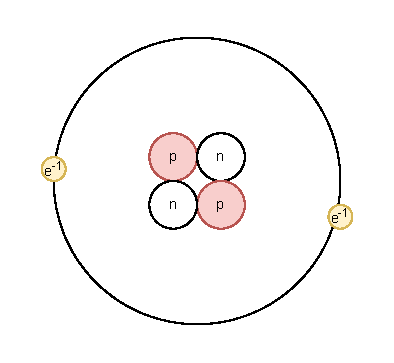
\includegraphics[width=0.5\columnwidth]{fig/helium.pdf}
    \caption{ヘリウム原子の構造}\label{helium-atom}
  \end{figure}
  \begin{myex}{ヘリウム原子の基底エネルギー(荒い近似)}{rough-helium}
    計算を行うと,ヘリウムの原子番号を$Z$として$\hat{H}^0$の基底波動関数,
    \begin{align}
      \psi = \cfrac{Z^3}{\pi a_0^3}\exp\qty(-Z\frac{r_1 + r_2}{a_0})\label{helium}
    \end{align}
    と$\hat{H}^0$の基底エネルギー,
    \begin{align}
      E = -8\ \r{Ry}\approx -108.8\ \r{eV}\label{helium-rough-min}
    \end{align}
    が求まる\footnote{
      $a_0 = \cfrac{4\pi\epsilon_0\hbar^2}{me^2} \approx 5.29\times 10^{-11}\ \r{m}$: Bohr半径
    }\footnote{
      $Z = 2$
    }\footnote{
      $\r{Ry} = \cfrac{\hbar^2}{2m\omega^2} \approx 13.6 \ \r{eV}$: Rydberg定数
    }.
  \end{myex}
  \begin{myex}{ヘリウム原子の基底エネルギー(変分法)}{}
    \exref{rough-helium}の結果とヘリウム原子の基底エネルギーの測定結果は$-78.6\ \r{eV}$と大きく異なっているため,相互作用の項を取り入れた近似を考える.
    \refe{helium}を試行関数$\psi(Z)$とする.
    $\psi(Z)$を用いてエネルギーを計算する.
    \begin{align}
      E(Z) &= \cfrac{\displaystyle\int\psi^{*}\hat{H}\psi \dd{\bm{r}_1}\dd{\bm{r}_2}}{\displaystyle\int\psi^{*}\psi \dd{\bm{r}_1}\dd{\bm{r}_2}} \\
      &= -2\qty(4Z - Z^2 - \cfrac{5}{8}Z)\ \r{Ry}\label{helium-energy-function} 
    \end{align}
    となる.\refe{helium-energy-function}が最小となるような$Z$を$Z_0$とすると$Z_0 = 27/16$であったので,
    \begin{align}
      E(Z) \geq E\qty(Z_0) = -77.5\ \r{eV}\label{helium-energy-varidation-min}
    \end{align}
    となった.\refe{helium-energy-varidation-min}と\refe{helium-rough-min}を比べると,変分法による近似の方が真の基底エネルギ$-78.6\ \r{eV}$に近い値が得られた\footnote{
      $Z_0 < 2$は遮蔽効果により有効電荷が$2e$より小さくなったことを意味する.
    }\footnote{
      積分の計算はDavid J. Griffith, \textit{Introduction to Quantum Mechanics}, pp. 333-334にある.
    }.
  \end{myex}
\end{document}
      \subsection{変分法の誤差の評価}
        \documentclass{report}
\usepackage{luatexja} % LuaTeXで日本語を使うためのパッケージ
\usepackage{luatexja-fontspec} % LuaTeX用の日本語フォント設定

% --- 数学関連 ---
\usepackage{amsmath, amssymb, amsfonts, mathtools, bm, amsthm} % 基本的な数学パッケージ
\usepackage{type1cm, upgreek} % 数式フォントとギリシャ文字
\usepackage{physics, mhchem} % 物理や化学の記号や式の表記を簡単にする

% --- 表関連 ---
\usepackage{multirow, longtable, tabularx, array, colortbl, dcolumn, diagbox} % 表のレイアウトを柔軟にする
\usepackage{tablefootnote, truthtable} % 表中に注釈を追加、真理値表
\usepackage{tabularray} % 高度な表組みレイアウト

% --- グラフィック関連 ---
\usepackage{tikz, graphicx} % 図の描画と画像の挿入
\usepackage{background} % ウォーターマークの設定
\usepackage{caption, subcaption} % 図や表のキャプション設定
\usepackage{float, here} % 図や表の位置指定

% --- レイアウトとページ設定 ---
\usepackage{fancyhdr} % ページヘッダー、フッター、余白の設定
\usepackage[top = 20truemm, bottom = 20truemm, left = 20truemm, right = 20truemm]{geometry}
\usepackage{fancybox, ascmac} % ボックスのデザイン

% --- 色とスタイル ---
\usepackage{xcolor, color, colortbl, tcolorbox} % 色とカラーボックス
\usepackage{listings, jvlisting} % コードの色付けとフォーマット

% --- 参考文献関連 ---
\usepackage{biblatex, usebib} % 参考文献の管理と挿入
\usepackage{url, hyperref} % URLとリンクの設定

% --- その他の便利なパッケージ ---
\usepackage{footmisc} % 脚注のカスタマイズ
\usepackage{multicol} % 複数段組
\usepackage{comment} % コメントアウトの拡張
\usepackage{siunitx} % 単位の表記
\usepackage{docmute}
% \usepackage{appendix}
% --- tcolorboxとtikzの設定 ---
\tcbuselibrary{theorems, breakable} % 定理のボックスと改ページ設定
\usetikzlibrary{decorations.markings, arrows.meta, calc} % tikzの装飾や矢印の設定

% --- 定理スタイルと数式設定 ---
\theoremstyle{definition} % 定義スタイル
\numberwithin{equation}{section} % 式番号をサブセクション単位でリセット

% --- hyperrefの設定 ---
\hypersetup{
  setpagesize = false,
  bookmarks = true,
  bookmarksdepth = tocdepth,
  bookmarksnumbered = true,
  colorlinks = false,
  pdftitle = {}, % PDFタイトル
  pdfsubject = {}, % PDFサブジェクト
  pdfauthor = {}, % PDF作者
  pdfkeywords = {} % PDFキーワード
}

% --- siunitxの設定 ---
\sisetup{
  table-format = 1.5, % 小数点以下の桁数
  table-number-alignment = center, % 数値の中央揃え
}

% --- 透かし画像の設定 --- 
\backgroundsetup{
  scale=0.5,                       % 画像のスケール
  % color=black,                   % 画像の色(透かし用に半透明が推奨)
  opacity=0.2,                   % 透かしの透明度(0が完全透明、1が完全不透明)
  angle=0,                       % 画像の角度
  position = current page.south east,  % ページの右下
  hshift=-6cm, % 右方向へのシフト(負の値で内側に移動)
  vshift=5cm,  % 上方向へのシフト(正の値で内側に移動)
  contents={
\includegraphics{./fig/appilogo-circular-full.png}} % 画像のパス
}

% --- その他の設定 ---
\allowdisplaybreaks % 数式の途中改ページ許可
\newcolumntype{t}{!{\vrule width 0.1pt}} % 新しいカラムタイプ
\newcolumntype{b}{!{\vrule width 1.5pt}} % 太いカラム
\UseTblrLibrary{amsmath, booktabs, counter, diagbox, functional, hook, html, nameref, siunitx, varwidth, zref} % tabularrayのライブラリ
\setlength{\columnseprule}{0.4pt} % カラム区切り線の太さ
\captionsetup[figure]{font = bf} % 図のキャプションの太字設定
\captionsetup[table]{font = bf} % 表のキャプションの太字設定
\captionsetup[lstlisting]{font = bf} % コードのキャプションの太字設定
\captionsetup[subfigure]{font = bf, labelformat = simple} % サブ図のキャプション設定
\setcounter{secnumdepth}{4} % セクションの深さ設定
\newcolumntype{d}{D{.}{.}{5}} % 数値のカラム
\newcolumntype{M}[1]{>{\centering\arraybackslash}m{#1}} % センター揃えのカラム
\DeclareMathOperator{\diag}{diag}
\everymath{\displaystyle} % 数式のスタイル
\newcommand{\inner}[2]{\left\langle #1, #2 \right\rangle}
\renewcommand{\figurename}{図}
\renewcommand{\i}{\mathrm{i}} % 複素数単位i
\renewcommand{\laplacian}{\grad^2} % ラプラシアンの記号
\renewcommand{\thesubfigure}{(\alph{subfigure})} % サブ図の番号形式
\newcommand{\m}[3]{\multicolumn{#1}{#2}{#3}} % マルチカラムのショートカット
\renewcommand{\r}[1]{\mathrm{#1}} % mathrmのショートカット
\newcommand{\e}{\mathrm{e}} % 自然対数の底e
\newcommand{\Ef}{E_{\mathrm{F}}} % フェルミエネルギー
\renewcommand{\c}{\si{\degreeCelsius}} % 摂氏記号
\renewcommand{\d}{\r{d}} % d記号
\renewcommand{\t}[1]{\texttt{#1}} % タイプライタフォント
\newcommand{\kb}{k_{\mathrm{B}}} % ボルツマン定数
% \renewcommand{\phi}{\varphi} % ϕをφに変更
\renewcommand{\epsilon}{\varepsilon}
\newcommand{\fullref}[1]{\textbf{\ref{#1} \nameref{#1}}}
\newcommand{\reff}[1]{\textbf{図\ref{#1}}} % 図参照のショートカット
\newcommand{\reft}[1]{\textbf{表\ref{#1}}} % 表参照のショートカット
\newcommand{\refe}[1]{\textbf{式\eqref{#1}}} % 式参照のショートカット
\newcommand{\refp}[1]{\textbf{コード\ref{#1}}} % コード参照のショートカット
\renewcommand{\lstlistingname}{コード} % コードリストの名前
\renewcommand{\theequation}{\thesection.\arabic{equation}} % 式番号の形式
\renewcommand{\footrulewidth}{0.4pt} % フッターの線
\newcommand{\mar}[1]{\textcircled{\scriptsize #1}} % 丸囲み文字
\newcommand{\combination}[2]{{}_{#1} \mathrm{C}_{#2}} % 組み合わせ
\newcommand{\thline}{\noalign{\hrule height 0.1pt}} % 細い横線
\newcommand{\bhline}{\noalign{\hrule height 1.5pt}} % 太い横線

% --- カスタム色定義 ---
\definecolor{burgundy}{rgb}{0.5, 0.0, 0.13} % バーガンディ色
\definecolor{charcoal}{rgb}{0.21, 0.27, 0.31} % チャコール色
\definecolor{forest}{rgb}{0.0, 0.35, 0} % 森の緑色

% --- カスタム定理環境の定義 ---
\newtcbtheorem[number within = chapter]{myexc}{練習問題}{
  fonttitle = \gtfamily\sffamily\bfseries\upshape,
  colframe = forest,
  colback = forest!2!white,
  rightrule = 1pt,
  leftrule = 1pt,
  bottomrule = 2pt,
  colbacktitle = forest,
  theorem style = standard,
  breakable,
  arc = 0pt,
}{exc-ref}
\newtcbtheorem[number within = chapter]{myprop}{命題}{
  fonttitle = \gtfamily\sffamily\bfseries\upshape,
  colframe = blue!50!black,
  colback = blue!50!black!2!white,
  rightrule = 1pt,
  leftrule = 1pt,
  bottomrule = 2pt,
  colbacktitle = blue!50!black,
  theorem style = standard,
  breakable,
  arc = 0pt
}{proposition-ref}
\newtcbtheorem[number within = chapter]{myrem}{注意}{
  fonttitle = \gtfamily\sffamily\bfseries\upshape,
  colframe = yellow!20!black,
  colback = yellow!50,
  rightrule = 1pt,
  leftrule = 1pt,
  bottomrule = 2pt,
  colbacktitle = yellow!20!black,
  theorem style = standard,
  breakable,
  arc = 0pt
}{remark-ref}
\newtcbtheorem[number within = chapter]{myex}{例題}{
  fonttitle = \gtfamily\sffamily\bfseries\upshape,
  colframe = black,
  colback = white,
  rightrule = 1pt,
  leftrule = 1pt,
  bottomrule = 2pt,
  colbacktitle = black,
  theorem style = standard,
  breakable,
  arc = 0pt
}{example-ref}
\newtcbtheorem[number within = chapter]{exc}{Requirement}{myexc}{exc-ref}
\newcommand{\rqref}[1]{{\bfseries\sffamily 練習問題 \ref{exc-ref:#1}}}
\newtcbtheorem[number within = chapter]{definition}{Definition}{mydef}{definition-ref}
\newcommand{\dfref}[1]{{\bfseries\sffamily 定義 \ref{definition-ref:#1}}}
\newtcbtheorem[number within = chapter]{prop}{命題}{myprop}{proposition-ref}
\newcommand{\prref}[1]{{\bfseries\sffamily 命題 \ref{proposition-ref:#1}}}
\newtcbtheorem[number within = chapter]{rem}{注意}{myrem}{remark-ref}
\newcommand{\rmref}[1]{{\bfseries\sffamily 注意 \ref{remark-ref:#1}}}
\newtcbtheorem[number within = chapter]{ex}{例題}{myex}{example-ref}
\newcommand{\exref}[1]{{\bfseries\sffamily 例題 \ref{example-ref:#1}}}
% --- 再定義コマンド ---
% \mathtoolsset{showonlyrefs=true} % 必要な式番号のみ表示
\pagestyle{fancy} % ヘッダー・フッターのスタイル設定
\chead{応用量子物性講義ノート} % 中央ヘッダー
% \rhead{}
\fancyhead[R]{\rightmark}
\renewcommand{\sectionmark}[1]{\markright{\thesection\ #1}}
\cfoot{\thepage} % 中央フッターにページ番号
\lhead{}
\rfoot{Yuto Masuda and Haruki Aoki} % 右フッターに名前
\setcounter{tocdepth}{4} % 目次の深さ
\makeatletter
\@addtoreset{equation}{section} % サブセクションごとに式番号をリセット
\makeatother

% --- メタ情報 ---
\title{応用量子物性講義ノート}
\date{更新日\today}
\author{Yuto Masuda and Haruki Aoki}

\begin{document}
  真の基底状態$\ket{E_0}$に第1励起状態$\ket{E_1}$を10\%含んだ試行関数$\ket{\psi} = \ket{E_0} + \cfrac{1}{10}\ket{E_1}$を使ってエネルギーを計算する.
  \begin{align}
    E(\psi) &= \frac{\mel{\psi}{\hat{H}}{\psi}}{\braket{\psi}} \\
    &= \cfrac{\bra{E_0}\hat{H}\ket{E_0} + \cfrac{1}{100}\mel{E_1}{\hat{H}}{E_1}}{1 + \cfrac{1}{100}} \\
    &= \cfrac{E_0 + 0.01E_1}{1.01}\\
    &\approx 0.99E_0 + 0.01E_1
  \end{align}
  試行関数で10\%含まれていた誤差がエネルギーでは1\%に収まっている.
  \begin{myex}{}{}
    無限井戸型ポテンシャル$[-a, a]$を考える.
    この問題を厳密に解けば$n$番目のエネルギー準位は,
    \begin{align}
      E_n = \cfrac{\hbar^2}{2m}\qty(\cfrac{n\pi}{2a})^2
    \end{align}
    と計算できるが,ここでは変分法を用いて近似解を求める.
    予想される試行関数の条件は
    \begin{itemize}
      \item $\psi(a) = \psi(-a) = 0$
      \item 節がない
    \end{itemize}
    である.よって今回は
    \begin{align}
      \psi(x) = a^2 - x^2
    \end{align}
    を採用する.この試行関数を用いたときの基底エネルギーを見積もれ.
    \tcblower
    \begin{align}
      E(\psi) &= \cfrac{\displaystyle \int_{-a}^{a}\qty(a^2 - x^2)\qty(-\frac{\hbar^2}{2m}\dv[2]{x})\qty(a^2 - x^2)\dd{x}}{\displaystyle \int_{-a}^{a}\qty(a^2 - x^2)^2\dd{x}} \\
      &= \cfrac{10}{\pi^2}E_1 \\
      &\approx 1.01E_1
    \end{align}
    真の基底エネルギー$E_1$に近い値が得られた\footnote{このくらいの計算が期末試験に出たことがある.}.
  \end{myex}
\end{document}
      \subsection{練習問題}
        \documentclass{report}
\usepackage{luatexja} % LuaTeXで日本語を使うためのパッケージ
\usepackage{luatexja-fontspec} % LuaTeX用の日本語フォント設定

% --- 数学関連 ---
\usepackage{amsmath, amssymb, amsfonts, mathtools, bm, amsthm} % 基本的な数学パッケージ
\usepackage{type1cm, upgreek} % 数式フォントとギリシャ文字
\usepackage{physics, mhchem} % 物理や化学の記号や式の表記を簡単にする

% --- 表関連 ---
\usepackage{multirow, longtable, tabularx, array, colortbl, dcolumn, diagbox} % 表のレイアウトを柔軟にする
\usepackage{tablefootnote, truthtable} % 表中に注釈を追加、真理値表
\usepackage{tabularray} % 高度な表組みレイアウト

% --- グラフィック関連 ---
\usepackage{tikz, graphicx} % 図の描画と画像の挿入
\usepackage{background} % ウォーターマークの設定
\usepackage{caption, subcaption} % 図や表のキャプション設定
\usepackage{float, here} % 図や表の位置指定

% --- レイアウトとページ設定 ---
\usepackage{fancyhdr} % ページヘッダー、フッター、余白の設定
\usepackage[top = 20truemm, bottom = 20truemm, left = 20truemm, right = 20truemm]{geometry}
\usepackage{fancybox, ascmac} % ボックスのデザイン

% --- 色とスタイル ---
\usepackage{xcolor, color, colortbl, tcolorbox} % 色とカラーボックス
\usepackage{listings, jvlisting} % コードの色付けとフォーマット

% --- 参考文献関連 ---
\usepackage{biblatex, usebib} % 参考文献の管理と挿入
\usepackage{url, hyperref} % URLとリンクの設定

% --- その他の便利なパッケージ ---
\usepackage{footmisc} % 脚注のカスタマイズ
\usepackage{multicol} % 複数段組
\usepackage{comment} % コメントアウトの拡張
\usepackage{siunitx} % 単位の表記
\usepackage{docmute}
% \usepackage{appendix}
% --- tcolorboxとtikzの設定 ---
\tcbuselibrary{theorems, breakable} % 定理のボックスと改ページ設定
\usetikzlibrary{decorations.markings, arrows.meta, calc} % tikzの装飾や矢印の設定

% --- 定理スタイルと数式設定 ---
\theoremstyle{definition} % 定義スタイル
\numberwithin{equation}{section} % 式番号をサブセクション単位でリセット

% --- hyperrefの設定 ---
\hypersetup{
  setpagesize = false,
  bookmarks = true,
  bookmarksdepth = tocdepth,
  bookmarksnumbered = true,
  colorlinks = false,
  pdftitle = {}, % PDFタイトル
  pdfsubject = {}, % PDFサブジェクト
  pdfauthor = {}, % PDF作者
  pdfkeywords = {} % PDFキーワード
}

% --- siunitxの設定 ---
\sisetup{
  table-format = 1.5, % 小数点以下の桁数
  table-number-alignment = center, % 数値の中央揃え
}

% --- 透かし画像の設定 --- 
\backgroundsetup{
  scale=0.5,                       % 画像のスケール
  % color=black,                   % 画像の色(透かし用に半透明が推奨)
  opacity=0.2,                   % 透かしの透明度(0が完全透明、1が完全不透明)
  angle=0,                       % 画像の角度
  position = current page.south east,  % ページの右下
  hshift=-6cm, % 右方向へのシフト(負の値で内側に移動)
  vshift=5cm,  % 上方向へのシフト(正の値で内側に移動)
  contents={
\includegraphics{./fig/appilogo-circular-full.png}} % 画像のパス
}

% --- その他の設定 ---
\allowdisplaybreaks % 数式の途中改ページ許可
\newcolumntype{t}{!{\vrule width 0.1pt}} % 新しいカラムタイプ
\newcolumntype{b}{!{\vrule width 1.5pt}} % 太いカラム
\UseTblrLibrary{amsmath, booktabs, counter, diagbox, functional, hook, html, nameref, siunitx, varwidth, zref} % tabularrayのライブラリ
\setlength{\columnseprule}{0.4pt} % カラム区切り線の太さ
\captionsetup[figure]{font = bf} % 図のキャプションの太字設定
\captionsetup[table]{font = bf} % 表のキャプションの太字設定
\captionsetup[lstlisting]{font = bf} % コードのキャプションの太字設定
\captionsetup[subfigure]{font = bf, labelformat = simple} % サブ図のキャプション設定
\setcounter{secnumdepth}{4} % セクションの深さ設定
\newcolumntype{d}{D{.}{.}{5}} % 数値のカラム
\newcolumntype{M}[1]{>{\centering\arraybackslash}m{#1}} % センター揃えのカラム
\DeclareMathOperator{\diag}{diag}
\everymath{\displaystyle} % 数式のスタイル
\newcommand{\inner}[2]{\left\langle #1, #2 \right\rangle}
\renewcommand{\figurename}{図}
\renewcommand{\i}{\mathrm{i}} % 複素数単位i
\renewcommand{\laplacian}{\grad^2} % ラプラシアンの記号
\renewcommand{\thesubfigure}{(\alph{subfigure})} % サブ図の番号形式
\newcommand{\m}[3]{\multicolumn{#1}{#2}{#3}} % マルチカラムのショートカット
\renewcommand{\r}[1]{\mathrm{#1}} % mathrmのショートカット
\newcommand{\e}{\mathrm{e}} % 自然対数の底e
\newcommand{\Ef}{E_{\mathrm{F}}} % フェルミエネルギー
\renewcommand{\c}{\si{\degreeCelsius}} % 摂氏記号
\renewcommand{\d}{\r{d}} % d記号
\renewcommand{\t}[1]{\texttt{#1}} % タイプライタフォント
\newcommand{\kb}{k_{\mathrm{B}}} % ボルツマン定数
% \renewcommand{\phi}{\varphi} % ϕをφに変更
\renewcommand{\epsilon}{\varepsilon}
\newcommand{\fullref}[1]{\textbf{\ref{#1} \nameref{#1}}}
\newcommand{\reff}[1]{\textbf{図\ref{#1}}} % 図参照のショートカット
\newcommand{\reft}[1]{\textbf{表\ref{#1}}} % 表参照のショートカット
\newcommand{\refe}[1]{\textbf{式\eqref{#1}}} % 式参照のショートカット
\newcommand{\refp}[1]{\textbf{コード\ref{#1}}} % コード参照のショートカット
\renewcommand{\lstlistingname}{コード} % コードリストの名前
\renewcommand{\theequation}{\thesection.\arabic{equation}} % 式番号の形式
\renewcommand{\footrulewidth}{0.4pt} % フッターの線
\newcommand{\mar}[1]{\textcircled{\scriptsize #1}} % 丸囲み文字
\newcommand{\combination}[2]{{}_{#1} \mathrm{C}_{#2}} % 組み合わせ
\newcommand{\thline}{\noalign{\hrule height 0.1pt}} % 細い横線
\newcommand{\bhline}{\noalign{\hrule height 1.5pt}} % 太い横線

% --- カスタム色定義 ---
\definecolor{burgundy}{rgb}{0.5, 0.0, 0.13} % バーガンディ色
\definecolor{charcoal}{rgb}{0.21, 0.27, 0.31} % チャコール色
\definecolor{forest}{rgb}{0.0, 0.35, 0} % 森の緑色

% --- カスタム定理環境の定義 ---
\newtcbtheorem[number within = chapter]{myexc}{練習問題}{
  fonttitle = \gtfamily\sffamily\bfseries\upshape,
  colframe = forest,
  colback = forest!2!white,
  rightrule = 1pt,
  leftrule = 1pt,
  bottomrule = 2pt,
  colbacktitle = forest,
  theorem style = standard,
  breakable,
  arc = 0pt,
}{exc-ref}
\newtcbtheorem[number within = chapter]{myprop}{命題}{
  fonttitle = \gtfamily\sffamily\bfseries\upshape,
  colframe = blue!50!black,
  colback = blue!50!black!2!white,
  rightrule = 1pt,
  leftrule = 1pt,
  bottomrule = 2pt,
  colbacktitle = blue!50!black,
  theorem style = standard,
  breakable,
  arc = 0pt
}{proposition-ref}
\newtcbtheorem[number within = chapter]{myrem}{注意}{
  fonttitle = \gtfamily\sffamily\bfseries\upshape,
  colframe = yellow!20!black,
  colback = yellow!50,
  rightrule = 1pt,
  leftrule = 1pt,
  bottomrule = 2pt,
  colbacktitle = yellow!20!black,
  theorem style = standard,
  breakable,
  arc = 0pt
}{remark-ref}
\newtcbtheorem[number within = chapter]{myex}{例題}{
  fonttitle = \gtfamily\sffamily\bfseries\upshape,
  colframe = black,
  colback = white,
  rightrule = 1pt,
  leftrule = 1pt,
  bottomrule = 2pt,
  colbacktitle = black,
  theorem style = standard,
  breakable,
  arc = 0pt
}{example-ref}
\newtcbtheorem[number within = chapter]{exc}{Requirement}{myexc}{exc-ref}
\newcommand{\rqref}[1]{{\bfseries\sffamily 練習問題 \ref{exc-ref:#1}}}
\newtcbtheorem[number within = chapter]{definition}{Definition}{mydef}{definition-ref}
\newcommand{\dfref}[1]{{\bfseries\sffamily 定義 \ref{definition-ref:#1}}}
\newtcbtheorem[number within = chapter]{prop}{命題}{myprop}{proposition-ref}
\newcommand{\prref}[1]{{\bfseries\sffamily 命題 \ref{proposition-ref:#1}}}
\newtcbtheorem[number within = chapter]{rem}{注意}{myrem}{remark-ref}
\newcommand{\rmref}[1]{{\bfseries\sffamily 注意 \ref{remark-ref:#1}}}
\newtcbtheorem[number within = chapter]{ex}{例題}{myex}{example-ref}
\newcommand{\exref}[1]{{\bfseries\sffamily 例題 \ref{example-ref:#1}}}
% --- 再定義コマンド ---
% \mathtoolsset{showonlyrefs=true} % 必要な式番号のみ表示
\pagestyle{fancy} % ヘッダー・フッターのスタイル設定
\chead{応用量子物性講義ノート} % 中央ヘッダー
% \rhead{}
\fancyhead[R]{\rightmark}
\renewcommand{\sectionmark}[1]{\markright{\thesection\ #1}}
\cfoot{\thepage} % 中央フッターにページ番号
\lhead{}
\rfoot{Yuto Masuda and Haruki Aoki} % 右フッターに名前
\setcounter{tocdepth}{4} % 目次の深さ
\makeatletter
\@addtoreset{equation}{section} % サブセクションごとに式番号をリセット
\makeatother

% --- メタ情報 ---
\title{応用量子物性講義ノート}
\date{更新日\today}
\author{Yuto Masuda and Haruki Aoki}

\begin{document}
  \begin{myexc}{Griffith Example 8.1}{}
    1次元調和振動子$\hat{H} = -\cfrac{\hbar^2}{2m}\dv[2]{x} + \cfrac{1}{2}m\omega^2 x^2$の基底エネルギーを見積もれ.
    ただし,試行関数を$\psi(x) = \qty(\cfrac{2b}{\pi})^{1/4}\e^{-bx^2}$とせよ.試行関数は規格化されている.
    \tcblower
    \begin{align}
      E(b) = \bra{\psi}\hat{H}\ket{\psi} &= \qty(\cfrac{2b}{\pi})^{1/2}\int_{-\infty}^{\infty}\e^{-bx^2}\qty(-\cfrac{\hbar^2}{2m}\dv[2]{x} + \cfrac{1}{2}m\omega^2x^2)\e^{-bx^2}\dd{x}\\
      &=\cfrac{\hbar^2b}{2m}+\cfrac{m\omega^2}{8b}
    \end{align}
    次に$E(b)$の最小値を求める.
    \begin{align}
      \dv{b}E(b_0) = \cfrac{\hbar^2}{2m} - \cfrac{m\omega^2}{8b_{0}^2} = 0\Rightarrow b_0 = \cfrac{m\omega}{2\hbar}
    \end{align}
    \begin{align}
      E(b_0) = \cfrac{1}{2}\hbar\omega
    \end{align}
    偶然にも試行関数は基底エネルギーの固有関数となっていたため,$E(b_0)$は基底エネルギーと一致した.
  \end{myexc}
  \begin{myexc}{Griffith Example 8.2}{}
    デルタ関数型ポテンシャル$\hat{H} - \dv[2]{x}-\alpha \delta(x)$の基底エネルギーを見積もれ.
    ただし,試行関数を$\psi(x) = \qty(\cfrac{2b}{\pi})^{1/4}\e^{-bx^2}$とせよ.試行関数は規格化されている.
    \tcblower
    \begin{align}
      \ev{V} &= -\alpha \qty(\cfrac{2b}{\pi})^{1/2}\int_{-\infty}^{\infty}\e^{-2bx^2}\delta(x)\dd{x} = -\alpha\qty(\cfrac{2b}{\pi})^{1/2}\\
      \ev{T} &= \cfrac{\hbar^2 b}{2m}\\
      E(b) &= \cfrac{\hbar^2 b}{2m} - \alpha\qty(\cfrac{2b}{\pi})^{1/2}
    \end{align}
    $E(b)$の最小値を求める.
    \begin{align}
      \dv{b}E(b_0) = \cfrac{\hbar^2}{2m} - \cfrac{\alpha}{\sqrt{2\pi b_0}} = 0\Rightarrow b_0=\cfrac{2m^2\alpha^2}{\pi\hbar^4}
    \end{align}
    よって,基底エネルギーの近似解として
    \begin{align}
      E(b_0) = -\cfrac{m\alpha^2}{\pi\hbar^2}
    \end{align}
    を得る\footnote{
      厳密解を求めることができ,$\psi(x) = \cfrac{\sqrt{m\alpha}}{\hbar}\e^{-m\alpha\abs{x}/\hbar^2},\ E_0 = -\cfrac{m\alpha^2}{2\hbar^2}$である.
    }.
  \end{myexc}
  \begin{myexc}{Griffith Example 8.3}{}
    $[0, a]$の無限井戸型ポテンシャルの基底エネルギーを見積もれ.ただし,試行関数を
    \begin{align}
      \psi(x)=
      \begin{dcases*}
        Ax & if $0 \leq x \leq a/2$ \\
        A(a - x) & if $a/2\leq x \leq a$ \\ 
        0 & otherwise 
      \end{dcases*}
    \end{align}
    とせよ.
    \tcblower
    規格化条件より,$A = \cfrac{2}{a}\sqrt{\cfrac{3}{a}}$を得る.波動関数の導関数は
    \begin{align}
      \dv[2]{\psi}{x} =
        \begin{dcases*}
          Ax & if $0 \leq x \leq a/2$ \\
          A(a - x) & if $a/2\leq x \leq a$ \\ 
          0 & otherwise 
        \end{dcases*}
    \end{align}
    である.よって,2次の微係数として
    \begin{align}
      \dv[2]{\psi}{x} = A\delta(x) - 2A\delta\qty(x - \cfrac{a}{2}) + A\delta(x - a)
    \end{align}
    を得る.したがって近似解は
    \begin{align}
      E &= \int_{0}^{a}\psi(x)\qty(-\cfrac{\hbar^2}{2m}\dv[2]{x})\psi(x)\dd{x}\\
      &= -\cfrac{\hbar^2}{2m}\int_{0}^{a} A\qty[\delta(x)-\delta\qty(x-\cfrac{a}{2}) + \delta(x - a)]\psi(x)\dd{x}\\
      &= \cfrac{12\hbar^2}{2ma^2}
    \end{align}
    である\footnote{
      厳密解は$E_0 = \cfrac{\pi^2\hbar^2}{2ma^2}$
    }.
  \end{myexc}
  \begin{myexc}{Griffith Problem8.4 (a)}{}
    試行関数$\ket{\psi}$が基底状態と直交するとき,つまり$\braket{\psi}{0}$のとき,
    \begin{align}
      E(\psi)\geq E_1
    \end{align}
    であることを示せ\footnote{
      例えば偶関数のポテンシャルに対し奇関数の試行関数で計算すれば第1励起状態のエネルギーの近似解が得られる.
    }.
    ただし$E_1$は第1励起状態のエネルギーである.$\ket{\psi}$は規格化されている.
    \tcblower
    \begin{proof}
      \begin{align}
        E(\psi) &= \sum_{k = 0}E_k\abs{\braket{\psi}{k}}^2 \\
        &= E_0\abs{\braket{\psi}{0}}^2 + \sum_{k = 1}\abs{\braket{\psi}{k}}^2 \\
        &= 0 + \sum_{k = 1}\abs{\braket{\psi}{k}}^2 \\
        &\geq E_1\sum_{k = 1}\abs{\braket{\psi}{k}}^2 = E_1
      \end{align}
    \end{proof}
  \end{myexc}
\end{document}

    \section{摂動I(定常摂動)}
      \documentclass{standalone}
\usepackage{luatexja} % LuaTeXで日本語を使うためのパッケージ
\usepackage{luatexja-fontspec} % LuaTeX用の日本語フォント設定

% --- 数学関連 ---
\usepackage{amsmath, amssymb, amsfonts, mathtools, bm, amsthm} % 基本的な数学パッケージ
\usepackage{type1cm, upgreek} % 数式フォントとギリシャ文字
\usepackage{physics, mhchem} % 物理や化学の記号や式の表記を簡単にする

% --- 表関連 ---
\usepackage{multirow, longtable, tabularx, array, colortbl, dcolumn, diagbox} % 表のレイアウトを柔軟にする
\usepackage{tablefootnote, truthtable} % 表中に注釈を追加、真理値表
\usepackage{tabularray} % 高度な表組みレイアウト

% --- グラフィック関連 ---
\usepackage{tikz, graphicx} % 図の描画と画像の挿入
\usepackage{background} % ウォーターマークの設定
\usepackage{caption, subcaption} % 図や表のキャプション設定
\usepackage{float, here} % 図や表の位置指定

% --- レイアウトとページ設定 ---
\usepackage{fancyhdr} % ページヘッダー、フッター、余白の設定
\usepackage[top = 20truemm, bottom = 20truemm, left = 20truemm, right = 20truemm]{geometry}
\usepackage{fancybox, ascmac} % ボックスのデザイン

% --- 色とスタイル ---
\usepackage{xcolor, color, colortbl, tcolorbox} % 色とカラーボックス
\usepackage{listings, jvlisting} % コードの色付けとフォーマット

% --- 参考文献関連 ---
\usepackage{biblatex, usebib} % 参考文献の管理と挿入
\usepackage{url, hyperref} % URLとリンクの設定

% --- その他の便利なパッケージ ---
\usepackage{footmisc} % 脚注のカスタマイズ
\usepackage{multicol} % 複数段組
\usepackage{comment} % コメントアウトの拡張
\usepackage{siunitx} % 単位の表記
\usepackage{docmute}
% \usepackage{appendix}
% --- tcolorboxとtikzの設定 ---
\tcbuselibrary{theorems, breakable} % 定理のボックスと改ページ設定
\usetikzlibrary{decorations.markings, arrows.meta, calc} % tikzの装飾や矢印の設定

% --- 定理スタイルと数式設定 ---
\theoremstyle{definition} % 定義スタイル
\numberwithin{equation}{section} % 式番号をサブセクション単位でリセット

% --- hyperrefの設定 ---
\hypersetup{
  setpagesize = false,
  bookmarks = true,
  bookmarksdepth = tocdepth,
  bookmarksnumbered = true,
  colorlinks = false,
  pdftitle = {}, % PDFタイトル
  pdfsubject = {}, % PDFサブジェクト
  pdfauthor = {}, % PDF作者
  pdfkeywords = {} % PDFキーワード
}

% --- siunitxの設定 ---
\sisetup{
  table-format = 1.5, % 小数点以下の桁数
  table-number-alignment = center, % 数値の中央揃え
}

% --- 透かし画像の設定 --- 
\backgroundsetup{
  scale=0.5,                       % 画像のスケール
  % color=black,                   % 画像の色(透かし用に半透明が推奨)
  opacity=0.2,                   % 透かしの透明度(0が完全透明、1が完全不透明)
  angle=0,                       % 画像の角度
  position = current page.south east,  % ページの右下
  hshift=-6cm, % 右方向へのシフト(負の値で内側に移動)
  vshift=5cm,  % 上方向へのシフト(正の値で内側に移動)
  contents={
\includegraphics{./fig/appilogo-circular-full.png}} % 画像のパス
}

% --- その他の設定 ---
\allowdisplaybreaks % 数式の途中改ページ許可
\newcolumntype{t}{!{\vrule width 0.1pt}} % 新しいカラムタイプ
\newcolumntype{b}{!{\vrule width 1.5pt}} % 太いカラム
\UseTblrLibrary{amsmath, booktabs, counter, diagbox, functional, hook, html, nameref, siunitx, varwidth, zref} % tabularrayのライブラリ
\setlength{\columnseprule}{0.4pt} % カラム区切り線の太さ
\captionsetup[figure]{font = bf} % 図のキャプションの太字設定
\captionsetup[table]{font = bf} % 表のキャプションの太字設定
\captionsetup[lstlisting]{font = bf} % コードのキャプションの太字設定
\captionsetup[subfigure]{font = bf, labelformat = simple} % サブ図のキャプション設定
\setcounter{secnumdepth}{4} % セクションの深さ設定
\newcolumntype{d}{D{.}{.}{5}} % 数値のカラム
\newcolumntype{M}[1]{>{\centering\arraybackslash}m{#1}} % センター揃えのカラム
\DeclareMathOperator{\diag}{diag}
\everymath{\displaystyle} % 数式のスタイル
\newcommand{\inner}[2]{\left\langle #1, #2 \right\rangle}
\renewcommand{\figurename}{図}
\renewcommand{\i}{\mathrm{i}} % 複素数単位i
\renewcommand{\laplacian}{\grad^2} % ラプラシアンの記号
\renewcommand{\thesubfigure}{(\alph{subfigure})} % サブ図の番号形式
\newcommand{\m}[3]{\multicolumn{#1}{#2}{#3}} % マルチカラムのショートカット
\renewcommand{\r}[1]{\mathrm{#1}} % mathrmのショートカット
\newcommand{\e}{\mathrm{e}} % 自然対数の底e
\newcommand{\Ef}{E_{\mathrm{F}}} % フェルミエネルギー
\renewcommand{\c}{\si{\degreeCelsius}} % 摂氏記号
\renewcommand{\d}{\r{d}} % d記号
\renewcommand{\t}[1]{\texttt{#1}} % タイプライタフォント
\newcommand{\kb}{k_{\mathrm{B}}} % ボルツマン定数
% \renewcommand{\phi}{\varphi} % ϕをφに変更
\renewcommand{\epsilon}{\varepsilon}
\newcommand{\fullref}[1]{\textbf{\ref{#1} \nameref{#1}}}
\newcommand{\reff}[1]{\textbf{図\ref{#1}}} % 図参照のショートカット
\newcommand{\reft}[1]{\textbf{表\ref{#1}}} % 表参照のショートカット
\newcommand{\refe}[1]{\textbf{式\eqref{#1}}} % 式参照のショートカット
\newcommand{\refp}[1]{\textbf{コード\ref{#1}}} % コード参照のショートカット
\renewcommand{\lstlistingname}{コード} % コードリストの名前
\renewcommand{\theequation}{\thesection.\arabic{equation}} % 式番号の形式
\renewcommand{\footrulewidth}{0.4pt} % フッターの線
\newcommand{\mar}[1]{\textcircled{\scriptsize #1}} % 丸囲み文字
\newcommand{\combination}[2]{{}_{#1} \mathrm{C}_{#2}} % 組み合わせ
\newcommand{\thline}{\noalign{\hrule height 0.1pt}} % 細い横線
\newcommand{\bhline}{\noalign{\hrule height 1.5pt}} % 太い横線

% --- カスタム色定義 ---
\definecolor{burgundy}{rgb}{0.5, 0.0, 0.13} % バーガンディ色
\definecolor{charcoal}{rgb}{0.21, 0.27, 0.31} % チャコール色
\definecolor{forest}{rgb}{0.0, 0.35, 0} % 森の緑色

% --- カスタム定理環境の定義 ---
\newtcbtheorem[number within = chapter]{myexc}{練習問題}{
  fonttitle = \gtfamily\sffamily\bfseries\upshape,
  colframe = forest,
  colback = forest!2!white,
  rightrule = 1pt,
  leftrule = 1pt,
  bottomrule = 2pt,
  colbacktitle = forest,
  theorem style = standard,
  breakable,
  arc = 0pt,
}{exc-ref}
\newtcbtheorem[number within = chapter]{myprop}{命題}{
  fonttitle = \gtfamily\sffamily\bfseries\upshape,
  colframe = blue!50!black,
  colback = blue!50!black!2!white,
  rightrule = 1pt,
  leftrule = 1pt,
  bottomrule = 2pt,
  colbacktitle = blue!50!black,
  theorem style = standard,
  breakable,
  arc = 0pt
}{proposition-ref}
\newtcbtheorem[number within = chapter]{myrem}{注意}{
  fonttitle = \gtfamily\sffamily\bfseries\upshape,
  colframe = yellow!20!black,
  colback = yellow!50,
  rightrule = 1pt,
  leftrule = 1pt,
  bottomrule = 2pt,
  colbacktitle = yellow!20!black,
  theorem style = standard,
  breakable,
  arc = 0pt
}{remark-ref}
\newtcbtheorem[number within = chapter]{myex}{例題}{
  fonttitle = \gtfamily\sffamily\bfseries\upshape,
  colframe = black,
  colback = white,
  rightrule = 1pt,
  leftrule = 1pt,
  bottomrule = 2pt,
  colbacktitle = black,
  theorem style = standard,
  breakable,
  arc = 0pt
}{example-ref}
\newtcbtheorem[number within = chapter]{exc}{Requirement}{myexc}{exc-ref}
\newcommand{\rqref}[1]{{\bfseries\sffamily 練習問題 \ref{exc-ref:#1}}}
\newtcbtheorem[number within = chapter]{definition}{Definition}{mydef}{definition-ref}
\newcommand{\dfref}[1]{{\bfseries\sffamily 定義 \ref{definition-ref:#1}}}
\newtcbtheorem[number within = chapter]{prop}{命題}{myprop}{proposition-ref}
\newcommand{\prref}[1]{{\bfseries\sffamily 命題 \ref{proposition-ref:#1}}}
\newtcbtheorem[number within = chapter]{rem}{注意}{myrem}{remark-ref}
\newcommand{\rmref}[1]{{\bfseries\sffamily 注意 \ref{remark-ref:#1}}}
\newtcbtheorem[number within = chapter]{ex}{例題}{myex}{example-ref}
\newcommand{\exref}[1]{{\bfseries\sffamily 例題 \ref{example-ref:#1}}}
% --- 再定義コマンド ---
% \mathtoolsset{showonlyrefs=true} % 必要な式番号のみ表示
\pagestyle{fancy} % ヘッダー・フッターのスタイル設定
\chead{応用量子物性講義ノート} % 中央ヘッダー
% \rhead{}
\fancyhead[R]{\rightmark}
\renewcommand{\sectionmark}[1]{\markright{\thesection\ #1}}
\cfoot{\thepage} % 中央フッターにページ番号
\lhead{}
\rfoot{Yuto Masuda and Haruki Aoki} % 右フッターに名前
\setcounter{tocdepth}{4} % 目次の深さ
\makeatletter
\@addtoreset{equation}{section} % サブセクションごとに式番号をリセット
\makeatother

% --- メタ情報 ---
\title{応用量子物性講義ノート}
\date{更新日\today}
\author{Yuto Masuda and Haruki Aoki}

\begin{document}
  Hamiltonianが時間に依存しない定常摂動(time-independent perturbation)を扱う.
\end{document}

      \subsection{準備}
        \documentclass{report}
\usepackage{luatexja} % LuaTeXで日本語を使うためのパッケージ
\usepackage{luatexja-fontspec} % LuaTeX用の日本語フォント設定

% --- 数学関連 ---
\usepackage{amsmath, amssymb, amsfonts, mathtools, bm, amsthm} % 基本的な数学パッケージ
\usepackage{type1cm, upgreek} % 数式フォントとギリシャ文字
\usepackage{physics, mhchem} % 物理や化学の記号や式の表記を簡単にする

% --- 表関連 ---
\usepackage{multirow, longtable, tabularx, array, colortbl, dcolumn, diagbox} % 表のレイアウトを柔軟にする
\usepackage{tablefootnote, truthtable} % 表中に注釈を追加、真理値表
\usepackage{tabularray} % 高度な表組みレイアウト

% --- グラフィック関連 ---
\usepackage{tikz, graphicx} % 図の描画と画像の挿入
\usepackage{background} % ウォーターマークの設定
\usepackage{caption, subcaption} % 図や表のキャプション設定
\usepackage{float, here} % 図や表の位置指定

% --- レイアウトとページ設定 ---
\usepackage{fancyhdr} % ページヘッダー、フッター、余白の設定
\usepackage[top = 20truemm, bottom = 20truemm, left = 20truemm, right = 20truemm]{geometry}
\usepackage{fancybox, ascmac} % ボックスのデザイン

% --- 色とスタイル ---
\usepackage{xcolor, color, colortbl, tcolorbox} % 色とカラーボックス
\usepackage{listings, jvlisting} % コードの色付けとフォーマット

% --- 参考文献関連 ---
\usepackage{biblatex, usebib} % 参考文献の管理と挿入
\usepackage{url, hyperref} % URLとリンクの設定

% --- その他の便利なパッケージ ---
\usepackage{footmisc} % 脚注のカスタマイズ
\usepackage{multicol} % 複数段組
\usepackage{comment} % コメントアウトの拡張
\usepackage{siunitx} % 単位の表記
\usepackage{docmute}
% \usepackage{appendix}
% --- tcolorboxとtikzの設定 ---
\tcbuselibrary{theorems, breakable} % 定理のボックスと改ページ設定
\usetikzlibrary{decorations.markings, arrows.meta, calc} % tikzの装飾や矢印の設定

% --- 定理スタイルと数式設定 ---
\theoremstyle{definition} % 定義スタイル
\numberwithin{equation}{section} % 式番号をサブセクション単位でリセット

% --- hyperrefの設定 ---
\hypersetup{
  setpagesize = false,
  bookmarks = true,
  bookmarksdepth = tocdepth,
  bookmarksnumbered = true,
  colorlinks = false,
  pdftitle = {}, % PDFタイトル
  pdfsubject = {}, % PDFサブジェクト
  pdfauthor = {}, % PDF作者
  pdfkeywords = {} % PDFキーワード
}

% --- siunitxの設定 ---
\sisetup{
  table-format = 1.5, % 小数点以下の桁数
  table-number-alignment = center, % 数値の中央揃え
}

% --- 透かし画像の設定 --- 
\backgroundsetup{
  scale=0.5,                       % 画像のスケール
  % color=black,                   % 画像の色(透かし用に半透明が推奨)
  opacity=0.2,                   % 透かしの透明度(0が完全透明、1が完全不透明)
  angle=0,                       % 画像の角度
  position = current page.south east,  % ページの右下
  hshift=-6cm, % 右方向へのシフト(負の値で内側に移動)
  vshift=5cm,  % 上方向へのシフト(正の値で内側に移動)
  contents={
\includegraphics{./fig/appilogo-circular-full.png}} % 画像のパス
}

% --- その他の設定 ---
\allowdisplaybreaks % 数式の途中改ページ許可
\newcolumntype{t}{!{\vrule width 0.1pt}} % 新しいカラムタイプ
\newcolumntype{b}{!{\vrule width 1.5pt}} % 太いカラム
\UseTblrLibrary{amsmath, booktabs, counter, diagbox, functional, hook, html, nameref, siunitx, varwidth, zref} % tabularrayのライブラリ
\setlength{\columnseprule}{0.4pt} % カラム区切り線の太さ
\captionsetup[figure]{font = bf} % 図のキャプションの太字設定
\captionsetup[table]{font = bf} % 表のキャプションの太字設定
\captionsetup[lstlisting]{font = bf} % コードのキャプションの太字設定
\captionsetup[subfigure]{font = bf, labelformat = simple} % サブ図のキャプション設定
\setcounter{secnumdepth}{4} % セクションの深さ設定
\newcolumntype{d}{D{.}{.}{5}} % 数値のカラム
\newcolumntype{M}[1]{>{\centering\arraybackslash}m{#1}} % センター揃えのカラム
\DeclareMathOperator{\diag}{diag}
\everymath{\displaystyle} % 数式のスタイル
\newcommand{\inner}[2]{\left\langle #1, #2 \right\rangle}
\renewcommand{\figurename}{図}
\renewcommand{\i}{\mathrm{i}} % 複素数単位i
\renewcommand{\laplacian}{\grad^2} % ラプラシアンの記号
\renewcommand{\thesubfigure}{(\alph{subfigure})} % サブ図の番号形式
\newcommand{\m}[3]{\multicolumn{#1}{#2}{#3}} % マルチカラムのショートカット
\renewcommand{\r}[1]{\mathrm{#1}} % mathrmのショートカット
\newcommand{\e}{\mathrm{e}} % 自然対数の底e
\newcommand{\Ef}{E_{\mathrm{F}}} % フェルミエネルギー
\renewcommand{\c}{\si{\degreeCelsius}} % 摂氏記号
\renewcommand{\d}{\r{d}} % d記号
\renewcommand{\t}[1]{\texttt{#1}} % タイプライタフォント
\newcommand{\kb}{k_{\mathrm{B}}} % ボルツマン定数
% \renewcommand{\phi}{\varphi} % ϕをφに変更
\renewcommand{\epsilon}{\varepsilon}
\newcommand{\fullref}[1]{\textbf{\ref{#1} \nameref{#1}}}
\newcommand{\reff}[1]{\textbf{図\ref{#1}}} % 図参照のショートカット
\newcommand{\reft}[1]{\textbf{表\ref{#1}}} % 表参照のショートカット
\newcommand{\refe}[1]{\textbf{式\eqref{#1}}} % 式参照のショートカット
\newcommand{\refp}[1]{\textbf{コード\ref{#1}}} % コード参照のショートカット
\renewcommand{\lstlistingname}{コード} % コードリストの名前
\renewcommand{\theequation}{\thesection.\arabic{equation}} % 式番号の形式
\renewcommand{\footrulewidth}{0.4pt} % フッターの線
\newcommand{\mar}[1]{\textcircled{\scriptsize #1}} % 丸囲み文字
\newcommand{\combination}[2]{{}_{#1} \mathrm{C}_{#2}} % 組み合わせ
\newcommand{\thline}{\noalign{\hrule height 0.1pt}} % 細い横線
\newcommand{\bhline}{\noalign{\hrule height 1.5pt}} % 太い横線

% --- カスタム色定義 ---
\definecolor{burgundy}{rgb}{0.5, 0.0, 0.13} % バーガンディ色
\definecolor{charcoal}{rgb}{0.21, 0.27, 0.31} % チャコール色
\definecolor{forest}{rgb}{0.0, 0.35, 0} % 森の緑色

% --- カスタム定理環境の定義 ---
\newtcbtheorem[number within = chapter]{myexc}{練習問題}{
  fonttitle = \gtfamily\sffamily\bfseries\upshape,
  colframe = forest,
  colback = forest!2!white,
  rightrule = 1pt,
  leftrule = 1pt,
  bottomrule = 2pt,
  colbacktitle = forest,
  theorem style = standard,
  breakable,
  arc = 0pt,
}{exc-ref}
\newtcbtheorem[number within = chapter]{myprop}{命題}{
  fonttitle = \gtfamily\sffamily\bfseries\upshape,
  colframe = blue!50!black,
  colback = blue!50!black!2!white,
  rightrule = 1pt,
  leftrule = 1pt,
  bottomrule = 2pt,
  colbacktitle = blue!50!black,
  theorem style = standard,
  breakable,
  arc = 0pt
}{proposition-ref}
\newtcbtheorem[number within = chapter]{myrem}{注意}{
  fonttitle = \gtfamily\sffamily\bfseries\upshape,
  colframe = yellow!20!black,
  colback = yellow!50,
  rightrule = 1pt,
  leftrule = 1pt,
  bottomrule = 2pt,
  colbacktitle = yellow!20!black,
  theorem style = standard,
  breakable,
  arc = 0pt
}{remark-ref}
\newtcbtheorem[number within = chapter]{myex}{例題}{
  fonttitle = \gtfamily\sffamily\bfseries\upshape,
  colframe = black,
  colback = white,
  rightrule = 1pt,
  leftrule = 1pt,
  bottomrule = 2pt,
  colbacktitle = black,
  theorem style = standard,
  breakable,
  arc = 0pt
}{example-ref}
\newtcbtheorem[number within = chapter]{exc}{Requirement}{myexc}{exc-ref}
\newcommand{\rqref}[1]{{\bfseries\sffamily 練習問題 \ref{exc-ref:#1}}}
\newtcbtheorem[number within = chapter]{definition}{Definition}{mydef}{definition-ref}
\newcommand{\dfref}[1]{{\bfseries\sffamily 定義 \ref{definition-ref:#1}}}
\newtcbtheorem[number within = chapter]{prop}{命題}{myprop}{proposition-ref}
\newcommand{\prref}[1]{{\bfseries\sffamily 命題 \ref{proposition-ref:#1}}}
\newtcbtheorem[number within = chapter]{rem}{注意}{myrem}{remark-ref}
\newcommand{\rmref}[1]{{\bfseries\sffamily 注意 \ref{remark-ref:#1}}}
\newtcbtheorem[number within = chapter]{ex}{例題}{myex}{example-ref}
\newcommand{\exref}[1]{{\bfseries\sffamily 例題 \ref{example-ref:#1}}}
% --- 再定義コマンド ---
% \mathtoolsset{showonlyrefs=true} % 必要な式番号のみ表示
\pagestyle{fancy} % ヘッダー・フッターのスタイル設定
\chead{応用量子物性講義ノート} % 中央ヘッダー
% \rhead{}
\fancyhead[R]{\rightmark}
\renewcommand{\sectionmark}[1]{\markright{\thesection\ #1}}
\cfoot{\thepage} % 中央フッターにページ番号
\lhead{}
\rfoot{Yuto Masuda and Haruki Aoki} % 右フッターに名前
\setcounter{tocdepth}{4} % 目次の深さ
\makeatletter
\@addtoreset{equation}{section} % サブセクションごとに式番号をリセット
\makeatother

% --- メタ情報 ---
\title{応用量子物性講義ノート}
\date{更新日\today}
\author{Yuto Masuda and Haruki Aoki}

\begin{document}
  摂動が無い状態のSch\"odinger方程式,
  \begin{equation}
    \hat{H}^{(0)}\ket{n^{(0)}}=E_0^{(0)}\ket{n^{(0)}}
  \end{equation}
  が厳密に解くことができるとする.
  ここに摂動$\hat{V}$を加わったこと\footnote{摂動の例: 光,電場}を考えると,摂動Hamiltonianを$\hat{V}$として,
  \begin{equation}
    \qty(\hat{H}^{(0)} + \hat{V})\ket{n} = E_n\ket{n}\label{perturbation-origin}
  \end{equation}
  とかける.摂動の大きさを表すパラメータを$\lambda$として\refe{perturbation-origin}を
  \begin{align}
    \hat{H} = \hat{H}^{(0)} + \lambda\hat{V}\label{perturbation-using-lambda}
  \end{align}
  とする.$\lambda\to 0$ならば明らかに,
  \begin{equation}
    \begin{cases}
      \ket{n}\to\ket{n^{(0)}}\\
      E_n\to E_n^{(0)}
    \end{cases}
  \end{equation}
  である.
  ここで,\refe{perturbation-using-lambda}の解が,%\footnote{$\hat{H},n,E$の肩の()を今後は省略する.}
  \begin{equation}
    \begin{cases}
      \ket{n} &= \ket{n^{(0)}} + \lambda\ket{n^{(1)}} + \lambda^2\ket{n^{(2)}} + \cdots \label{n-en-expantion} \\
      E_n &= E_n^{(0)} + \lambda E_n^{(1)} + \lambda^2 E_n^{(2)} + \cdots 
    \end{cases}
  \end{equation}
  と書けたとする.
  $\ket{n^{(1)}}$,$\ket{n^{(2)}}$,$E_n^{(1)}$,$E_n^{(2)}$を考える.
  規格化条件として
  \begin{equation}
    \braket{n^{(0)}}{n} = 1
  \end{equation}
  を定める.
  \refe{n-en-expantion}を\refe{perturbation-using-lambda}に代入して,$\lambda$の次数ごとにまとめると,
  \begin{align}
    &(E_n^{(0)} - \hat{H}^{(0)})\ket{n^{(0)}} = 0 \label{0-order} \\ 
    &(E_n^{(0)} - \hat{H}^{(0)})\ket{n^{(1)}} + E_n^{(1)}\ket{n^{(0)}} = \hat{V}\ket{n^{(0)}} \label{1st-perturbation} \\
    &(E_n^{(0)} - \hat{H}^{(0)})\ket{n^{(2)}} + E_n^{(1)}\ket{n^{(1)}} + E_n^{(2)}\ket{n^{(0)}} = \hat{V}\ket{n^{(1)}} \label{2nd-perturbation}\\
  \end{align}
  を得る.
\end{document}

      \subsection{1次摂動}
        \documentclass{report}
\usepackage{luatexja} % LuaTeXで日本語を使うためのパッケージ
\usepackage{luatexja-fontspec} % LuaTeX用の日本語フォント設定

% --- 数学関連 ---
\usepackage{amsmath, amssymb, amsfonts, mathtools, bm, amsthm} % 基本的な数学パッケージ
\usepackage{type1cm, upgreek} % 数式フォントとギリシャ文字
\usepackage{physics, mhchem} % 物理や化学の記号や式の表記を簡単にする

% --- 表関連 ---
\usepackage{multirow, longtable, tabularx, array, colortbl, dcolumn, diagbox} % 表のレイアウトを柔軟にする
\usepackage{tablefootnote, truthtable} % 表中に注釈を追加、真理値表
\usepackage{tabularray} % 高度な表組みレイアウト

% --- グラフィック関連 ---
\usepackage{tikz, graphicx} % 図の描画と画像の挿入
\usepackage{background} % ウォーターマークの設定
\usepackage{caption, subcaption} % 図や表のキャプション設定
\usepackage{float, here} % 図や表の位置指定

% --- レイアウトとページ設定 ---
\usepackage{fancyhdr} % ページヘッダー、フッター、余白の設定
\usepackage[top = 20truemm, bottom = 20truemm, left = 20truemm, right = 20truemm]{geometry}
\usepackage{fancybox, ascmac} % ボックスのデザイン

% --- 色とスタイル ---
\usepackage{xcolor, color, colortbl, tcolorbox} % 色とカラーボックス
\usepackage{listings, jvlisting} % コードの色付けとフォーマット

% --- 参考文献関連 ---
\usepackage{biblatex, usebib} % 参考文献の管理と挿入
\usepackage{url, hyperref} % URLとリンクの設定

% --- その他の便利なパッケージ ---
\usepackage{footmisc} % 脚注のカスタマイズ
\usepackage{multicol} % 複数段組
\usepackage{comment} % コメントアウトの拡張
\usepackage{siunitx} % 単位の表記
\usepackage{docmute}
% \usepackage{appendix}
% --- tcolorboxとtikzの設定 ---
\tcbuselibrary{theorems, breakable} % 定理のボックスと改ページ設定
\usetikzlibrary{decorations.markings, arrows.meta, calc} % tikzの装飾や矢印の設定

% --- 定理スタイルと数式設定 ---
\theoremstyle{definition} % 定義スタイル
\numberwithin{equation}{section} % 式番号をサブセクション単位でリセット

% --- hyperrefの設定 ---
\hypersetup{
  setpagesize = false,
  bookmarks = true,
  bookmarksdepth = tocdepth,
  bookmarksnumbered = true,
  colorlinks = false,
  pdftitle = {}, % PDFタイトル
  pdfsubject = {}, % PDFサブジェクト
  pdfauthor = {}, % PDF作者
  pdfkeywords = {} % PDFキーワード
}

% --- siunitxの設定 ---
\sisetup{
  table-format = 1.5, % 小数点以下の桁数
  table-number-alignment = center, % 数値の中央揃え
}

% --- 透かし画像の設定 --- 
\backgroundsetup{
  scale=0.5,                       % 画像のスケール
  % color=black,                   % 画像の色(透かし用に半透明が推奨)
  opacity=0.2,                   % 透かしの透明度(0が完全透明、1が完全不透明)
  angle=0,                       % 画像の角度
  position = current page.south east,  % ページの右下
  hshift=-6cm, % 右方向へのシフト(負の値で内側に移動)
  vshift=5cm,  % 上方向へのシフト(正の値で内側に移動)
  contents={
\includegraphics{./fig/appilogo-circular-full.png}} % 画像のパス
}

% --- その他の設定 ---
\allowdisplaybreaks % 数式の途中改ページ許可
\newcolumntype{t}{!{\vrule width 0.1pt}} % 新しいカラムタイプ
\newcolumntype{b}{!{\vrule width 1.5pt}} % 太いカラム
\UseTblrLibrary{amsmath, booktabs, counter, diagbox, functional, hook, html, nameref, siunitx, varwidth, zref} % tabularrayのライブラリ
\setlength{\columnseprule}{0.4pt} % カラム区切り線の太さ
\captionsetup[figure]{font = bf} % 図のキャプションの太字設定
\captionsetup[table]{font = bf} % 表のキャプションの太字設定
\captionsetup[lstlisting]{font = bf} % コードのキャプションの太字設定
\captionsetup[subfigure]{font = bf, labelformat = simple} % サブ図のキャプション設定
\setcounter{secnumdepth}{4} % セクションの深さ設定
\newcolumntype{d}{D{.}{.}{5}} % 数値のカラム
\newcolumntype{M}[1]{>{\centering\arraybackslash}m{#1}} % センター揃えのカラム
\DeclareMathOperator{\diag}{diag}
\everymath{\displaystyle} % 数式のスタイル
\newcommand{\inner}[2]{\left\langle #1, #2 \right\rangle}
\renewcommand{\figurename}{図}
\renewcommand{\i}{\mathrm{i}} % 複素数単位i
\renewcommand{\laplacian}{\grad^2} % ラプラシアンの記号
\renewcommand{\thesubfigure}{(\alph{subfigure})} % サブ図の番号形式
\newcommand{\m}[3]{\multicolumn{#1}{#2}{#3}} % マルチカラムのショートカット
\renewcommand{\r}[1]{\mathrm{#1}} % mathrmのショートカット
\newcommand{\e}{\mathrm{e}} % 自然対数の底e
\newcommand{\Ef}{E_{\mathrm{F}}} % フェルミエネルギー
\renewcommand{\c}{\si{\degreeCelsius}} % 摂氏記号
\renewcommand{\d}{\r{d}} % d記号
\renewcommand{\t}[1]{\texttt{#1}} % タイプライタフォント
\newcommand{\kb}{k_{\mathrm{B}}} % ボルツマン定数
% \renewcommand{\phi}{\varphi} % ϕをφに変更
\renewcommand{\epsilon}{\varepsilon}
\newcommand{\fullref}[1]{\textbf{\ref{#1} \nameref{#1}}}
\newcommand{\reff}[1]{\textbf{図\ref{#1}}} % 図参照のショートカット
\newcommand{\reft}[1]{\textbf{表\ref{#1}}} % 表参照のショートカット
\newcommand{\refe}[1]{\textbf{式\eqref{#1}}} % 式参照のショートカット
\newcommand{\refp}[1]{\textbf{コード\ref{#1}}} % コード参照のショートカット
\renewcommand{\lstlistingname}{コード} % コードリストの名前
\renewcommand{\theequation}{\thesection.\arabic{equation}} % 式番号の形式
\renewcommand{\footrulewidth}{0.4pt} % フッターの線
\newcommand{\mar}[1]{\textcircled{\scriptsize #1}} % 丸囲み文字
\newcommand{\combination}[2]{{}_{#1} \mathrm{C}_{#2}} % 組み合わせ
\newcommand{\thline}{\noalign{\hrule height 0.1pt}} % 細い横線
\newcommand{\bhline}{\noalign{\hrule height 1.5pt}} % 太い横線

% --- カスタム色定義 ---
\definecolor{burgundy}{rgb}{0.5, 0.0, 0.13} % バーガンディ色
\definecolor{charcoal}{rgb}{0.21, 0.27, 0.31} % チャコール色
\definecolor{forest}{rgb}{0.0, 0.35, 0} % 森の緑色

% --- カスタム定理環境の定義 ---
\newtcbtheorem[number within = chapter]{myexc}{練習問題}{
  fonttitle = \gtfamily\sffamily\bfseries\upshape,
  colframe = forest,
  colback = forest!2!white,
  rightrule = 1pt,
  leftrule = 1pt,
  bottomrule = 2pt,
  colbacktitle = forest,
  theorem style = standard,
  breakable,
  arc = 0pt,
}{exc-ref}
\newtcbtheorem[number within = chapter]{myprop}{命題}{
  fonttitle = \gtfamily\sffamily\bfseries\upshape,
  colframe = blue!50!black,
  colback = blue!50!black!2!white,
  rightrule = 1pt,
  leftrule = 1pt,
  bottomrule = 2pt,
  colbacktitle = blue!50!black,
  theorem style = standard,
  breakable,
  arc = 0pt
}{proposition-ref}
\newtcbtheorem[number within = chapter]{myrem}{注意}{
  fonttitle = \gtfamily\sffamily\bfseries\upshape,
  colframe = yellow!20!black,
  colback = yellow!50,
  rightrule = 1pt,
  leftrule = 1pt,
  bottomrule = 2pt,
  colbacktitle = yellow!20!black,
  theorem style = standard,
  breakable,
  arc = 0pt
}{remark-ref}
\newtcbtheorem[number within = chapter]{myex}{例題}{
  fonttitle = \gtfamily\sffamily\bfseries\upshape,
  colframe = black,
  colback = white,
  rightrule = 1pt,
  leftrule = 1pt,
  bottomrule = 2pt,
  colbacktitle = black,
  theorem style = standard,
  breakable,
  arc = 0pt
}{example-ref}
\newtcbtheorem[number within = chapter]{exc}{Requirement}{myexc}{exc-ref}
\newcommand{\rqref}[1]{{\bfseries\sffamily 練習問題 \ref{exc-ref:#1}}}
\newtcbtheorem[number within = chapter]{definition}{Definition}{mydef}{definition-ref}
\newcommand{\dfref}[1]{{\bfseries\sffamily 定義 \ref{definition-ref:#1}}}
\newtcbtheorem[number within = chapter]{prop}{命題}{myprop}{proposition-ref}
\newcommand{\prref}[1]{{\bfseries\sffamily 命題 \ref{proposition-ref:#1}}}
\newtcbtheorem[number within = chapter]{rem}{注意}{myrem}{remark-ref}
\newcommand{\rmref}[1]{{\bfseries\sffamily 注意 \ref{remark-ref:#1}}}
\newtcbtheorem[number within = chapter]{ex}{例題}{myex}{example-ref}
\newcommand{\exref}[1]{{\bfseries\sffamily 例題 \ref{example-ref:#1}}}
% --- 再定義コマンド ---
% \mathtoolsset{showonlyrefs=true} % 必要な式番号のみ表示
\pagestyle{fancy} % ヘッダー・フッターのスタイル設定
\chead{応用量子物性講義ノート} % 中央ヘッダー
% \rhead{}
\fancyhead[R]{\rightmark}
\renewcommand{\sectionmark}[1]{\markright{\thesection\ #1}}
\cfoot{\thepage} % 中央フッターにページ番号
\lhead{}
\rfoot{Yuto Masuda and Haruki Aoki} % 右フッターに名前
\setcounter{tocdepth}{4} % 目次の深さ
\makeatletter
\@addtoreset{equation}{section} % サブセクションごとに式番号をリセット
\makeatother

% --- メタ情報 ---
\title{応用量子物性講義ノート}
\date{更新日\today}
\author{Yuto Masuda and Haruki Aoki}

\begin{document}
  まずエネルギー補正$E_n^{(1)}$について考える.
  \refe{1st-perturbation}の両辺に$\bra{n^{(1)}}$を作用すると,
  \begin{align}
    \ev**{(E_n^{(0)} - \hat{H}^{(0)})}{n^{(1)}} + \mel**{n^{(1)}}{E_n^{(1)}}{n^{(0)}} &= \mel{n^{(1)}}{\hat{V}}{n^{(0)}} \\ 
    \Leftrightarrow E_n^{(0)}\braket{n^{(1)}} - \ev**{\hat{H}^{(0)}}{n^{(1)}} + E_n^{(1)}\braket{n^{(1)}}{n^{(0)}} &= \mel{n^{(1)}}{\hat{V}}{n^{(0)}} \\ 
    \Leftrightarrow 0 + E_n^{(1)}\braket{n^{(0)}} &= \ev**{\hat{V}}{n^{(0)}} \\ 
    \Leftrightarrow E_n^{(1)} &= \ev**{\hat{V}}{n^{(0)}}
  \end{align}
  を得る.よって,1次摂動によるエネルギー補正は
  \begin{itembox}[l]{1次摂動によるエネルギー補正}
    \begin{align}
      E_n^{(1)} = \ev**{\hat{V}}{n^{(0)}}
    \end{align}
  \end{itembox}
  である.
  \par
  次に固有ベクトル$\ket{n^{(1)}}$の補正を求める.
  \refe{1st-perturbation}の両辺に$\bra{m^{(0)}}$,ただし$m\neq n$を作用すると,
  \begin{align}
    \mel**{m^{(0)}}{(E_n^{(0)} - \hat{H}^{(0)})}{n^{(1)}} + \mel**{m^{(0)}}{E_n^{(1)}}{n^{(0)}} &= \mel**{m^{(0)}}{\hat{V}}{n^{(0)}} \\ 
    E_n^{(0)}\braket{m^{(0)}}{n^{(1)}} - E_m^{(0)}\braket{m^{(0)}}{n^{(1)}} + 0 &= \mel**{m^{(0)}}{\hat{V}}{n^{(0)}}\\
    \braket{m^{(0)}}{n^{(1)}} = \mel**{m^{(0)}}{\hat{V}}{n^{(0)}} \qty(E_n^{(0)} - E_m^{(0)}) \label{1st-perturbation-prep}\\
  \end{align}
  ただし,エネルギー縮退は無く,
  \begin{align}
    E_n^{(0)}-E_m^{(0)} \neq 0\label{no-degeneracy}
  \end{align}
  とする.
  ところで,Hermite演算子である$\hat{H}^{(0)}$の固有ベクトルに関する完全性より,
  \begin{align}
    I = \sum_{m}\ketbra{m^{(0)}}{m^{(0)}}\label{completeness}
  \end{align}
  であるから,\refe{completeness}の両辺に右から$\ket{n^{(1)}}$をかけて,
  \begin{align}
    \ket{n^{(1)}} = \sum_{m}\ket{m^{(0)}}\braket{m^{(0)}}{n^{(1)}}\label{n1-completeness-expantion}
  \end{align}
  を得る.\refe{n1-completeness-expantion}を\refe{1st-perturbation-prep}に代入すると,
  \begin{itembox}[l]{1次摂動による固有ベクトル補正}
    \begin{align}
      \ket{n^{(1)}} = \sum_{m\neq n}\cfrac{\mel**{m^{(0)}}{\hat{V}}{n^{(0)}}}{E_n^{(0)} - E_m^{(0)}}\ket{m^{(0)}}\label{1st-order-eigenvector}
    \end{align}
  \end{itembox}
  を得る.
\end{document}

      \subsection{(1次摂動の例題)ヘリウム原子}
        \documentclass{report}
\usepackage{luatexja} % LuaTeXで日本語を使うためのパッケージ
\usepackage{luatexja-fontspec} % LuaTeX用の日本語フォント設定

% --- 数学関連 ---
\usepackage{amsmath, amssymb, amsfonts, mathtools, bm, amsthm} % 基本的な数学パッケージ
\usepackage{type1cm, upgreek} % 数式フォントとギリシャ文字
\usepackage{physics, mhchem} % 物理や化学の記号や式の表記を簡単にする

% --- 表関連 ---
\usepackage{multirow, longtable, tabularx, array, colortbl, dcolumn, diagbox} % 表のレイアウトを柔軟にする
\usepackage{tablefootnote, truthtable} % 表中に注釈を追加、真理値表
\usepackage{tabularray} % 高度な表組みレイアウト

% --- グラフィック関連 ---
\usepackage{tikz, graphicx} % 図の描画と画像の挿入
\usepackage{background} % ウォーターマークの設定
\usepackage{caption, subcaption} % 図や表のキャプション設定
\usepackage{float, here} % 図や表の位置指定

% --- レイアウトとページ設定 ---
\usepackage{fancyhdr} % ページヘッダー、フッター、余白の設定
\usepackage[top = 20truemm, bottom = 20truemm, left = 20truemm, right = 20truemm]{geometry}
\usepackage{fancybox, ascmac} % ボックスのデザイン

% --- 色とスタイル ---
\usepackage{xcolor, color, colortbl, tcolorbox} % 色とカラーボックス
\usepackage{listings, jvlisting} % コードの色付けとフォーマット

% --- 参考文献関連 ---
\usepackage{biblatex, usebib} % 参考文献の管理と挿入
\usepackage{url, hyperref} % URLとリンクの設定

% --- その他の便利なパッケージ ---
\usepackage{footmisc} % 脚注のカスタマイズ
\usepackage{multicol} % 複数段組
\usepackage{comment} % コメントアウトの拡張
\usepackage{siunitx} % 単位の表記
\usepackage{docmute}
% \usepackage{appendix}
% --- tcolorboxとtikzの設定 ---
\tcbuselibrary{theorems, breakable} % 定理のボックスと改ページ設定
\usetikzlibrary{decorations.markings, arrows.meta, calc} % tikzの装飾や矢印の設定

% --- 定理スタイルと数式設定 ---
\theoremstyle{definition} % 定義スタイル
\numberwithin{equation}{section} % 式番号をサブセクション単位でリセット

% --- hyperrefの設定 ---
\hypersetup{
  setpagesize = false,
  bookmarks = true,
  bookmarksdepth = tocdepth,
  bookmarksnumbered = true,
  colorlinks = false,
  pdftitle = {}, % PDFタイトル
  pdfsubject = {}, % PDFサブジェクト
  pdfauthor = {}, % PDF作者
  pdfkeywords = {} % PDFキーワード
}

% --- siunitxの設定 ---
\sisetup{
  table-format = 1.5, % 小数点以下の桁数
  table-number-alignment = center, % 数値の中央揃え
}

% --- 透かし画像の設定 --- 
\backgroundsetup{
  scale=0.5,                       % 画像のスケール
  % color=black,                   % 画像の色(透かし用に半透明が推奨)
  opacity=0.2,                   % 透かしの透明度(0が完全透明、1が完全不透明)
  angle=0,                       % 画像の角度
  position = current page.south east,  % ページの右下
  hshift=-6cm, % 右方向へのシフト(負の値で内側に移動)
  vshift=5cm,  % 上方向へのシフト(正の値で内側に移動)
  contents={
\includegraphics{./fig/appilogo-circular-full.png}} % 画像のパス
}

% --- その他の設定 ---
\allowdisplaybreaks % 数式の途中改ページ許可
\newcolumntype{t}{!{\vrule width 0.1pt}} % 新しいカラムタイプ
\newcolumntype{b}{!{\vrule width 1.5pt}} % 太いカラム
\UseTblrLibrary{amsmath, booktabs, counter, diagbox, functional, hook, html, nameref, siunitx, varwidth, zref} % tabularrayのライブラリ
\setlength{\columnseprule}{0.4pt} % カラム区切り線の太さ
\captionsetup[figure]{font = bf} % 図のキャプションの太字設定
\captionsetup[table]{font = bf} % 表のキャプションの太字設定
\captionsetup[lstlisting]{font = bf} % コードのキャプションの太字設定
\captionsetup[subfigure]{font = bf, labelformat = simple} % サブ図のキャプション設定
\setcounter{secnumdepth}{4} % セクションの深さ設定
\newcolumntype{d}{D{.}{.}{5}} % 数値のカラム
\newcolumntype{M}[1]{>{\centering\arraybackslash}m{#1}} % センター揃えのカラム
\DeclareMathOperator{\diag}{diag}
\everymath{\displaystyle} % 数式のスタイル
\newcommand{\inner}[2]{\left\langle #1, #2 \right\rangle}
\renewcommand{\figurename}{図}
\renewcommand{\i}{\mathrm{i}} % 複素数単位i
\renewcommand{\laplacian}{\grad^2} % ラプラシアンの記号
\renewcommand{\thesubfigure}{(\alph{subfigure})} % サブ図の番号形式
\newcommand{\m}[3]{\multicolumn{#1}{#2}{#3}} % マルチカラムのショートカット
\renewcommand{\r}[1]{\mathrm{#1}} % mathrmのショートカット
\newcommand{\e}{\mathrm{e}} % 自然対数の底e
\newcommand{\Ef}{E_{\mathrm{F}}} % フェルミエネルギー
\renewcommand{\c}{\si{\degreeCelsius}} % 摂氏記号
\renewcommand{\d}{\r{d}} % d記号
\renewcommand{\t}[1]{\texttt{#1}} % タイプライタフォント
\newcommand{\kb}{k_{\mathrm{B}}} % ボルツマン定数
% \renewcommand{\phi}{\varphi} % ϕをφに変更
\renewcommand{\epsilon}{\varepsilon}
\newcommand{\fullref}[1]{\textbf{\ref{#1} \nameref{#1}}}
\newcommand{\reff}[1]{\textbf{図\ref{#1}}} % 図参照のショートカット
\newcommand{\reft}[1]{\textbf{表\ref{#1}}} % 表参照のショートカット
\newcommand{\refe}[1]{\textbf{式\eqref{#1}}} % 式参照のショートカット
\newcommand{\refp}[1]{\textbf{コード\ref{#1}}} % コード参照のショートカット
\renewcommand{\lstlistingname}{コード} % コードリストの名前
\renewcommand{\theequation}{\thesection.\arabic{equation}} % 式番号の形式
\renewcommand{\footrulewidth}{0.4pt} % フッターの線
\newcommand{\mar}[1]{\textcircled{\scriptsize #1}} % 丸囲み文字
\newcommand{\combination}[2]{{}_{#1} \mathrm{C}_{#2}} % 組み合わせ
\newcommand{\thline}{\noalign{\hrule height 0.1pt}} % 細い横線
\newcommand{\bhline}{\noalign{\hrule height 1.5pt}} % 太い横線

% --- カスタム色定義 ---
\definecolor{burgundy}{rgb}{0.5, 0.0, 0.13} % バーガンディ色
\definecolor{charcoal}{rgb}{0.21, 0.27, 0.31} % チャコール色
\definecolor{forest}{rgb}{0.0, 0.35, 0} % 森の緑色

% --- カスタム定理環境の定義 ---
\newtcbtheorem[number within = chapter]{myexc}{練習問題}{
  fonttitle = \gtfamily\sffamily\bfseries\upshape,
  colframe = forest,
  colback = forest!2!white,
  rightrule = 1pt,
  leftrule = 1pt,
  bottomrule = 2pt,
  colbacktitle = forest,
  theorem style = standard,
  breakable,
  arc = 0pt,
}{exc-ref}
\newtcbtheorem[number within = chapter]{myprop}{命題}{
  fonttitle = \gtfamily\sffamily\bfseries\upshape,
  colframe = blue!50!black,
  colback = blue!50!black!2!white,
  rightrule = 1pt,
  leftrule = 1pt,
  bottomrule = 2pt,
  colbacktitle = blue!50!black,
  theorem style = standard,
  breakable,
  arc = 0pt
}{proposition-ref}
\newtcbtheorem[number within = chapter]{myrem}{注意}{
  fonttitle = \gtfamily\sffamily\bfseries\upshape,
  colframe = yellow!20!black,
  colback = yellow!50,
  rightrule = 1pt,
  leftrule = 1pt,
  bottomrule = 2pt,
  colbacktitle = yellow!20!black,
  theorem style = standard,
  breakable,
  arc = 0pt
}{remark-ref}
\newtcbtheorem[number within = chapter]{myex}{例題}{
  fonttitle = \gtfamily\sffamily\bfseries\upshape,
  colframe = black,
  colback = white,
  rightrule = 1pt,
  leftrule = 1pt,
  bottomrule = 2pt,
  colbacktitle = black,
  theorem style = standard,
  breakable,
  arc = 0pt
}{example-ref}
\newtcbtheorem[number within = chapter]{exc}{Requirement}{myexc}{exc-ref}
\newcommand{\rqref}[1]{{\bfseries\sffamily 練習問題 \ref{exc-ref:#1}}}
\newtcbtheorem[number within = chapter]{definition}{Definition}{mydef}{definition-ref}
\newcommand{\dfref}[1]{{\bfseries\sffamily 定義 \ref{definition-ref:#1}}}
\newtcbtheorem[number within = chapter]{prop}{命題}{myprop}{proposition-ref}
\newcommand{\prref}[1]{{\bfseries\sffamily 命題 \ref{proposition-ref:#1}}}
\newtcbtheorem[number within = chapter]{rem}{注意}{myrem}{remark-ref}
\newcommand{\rmref}[1]{{\bfseries\sffamily 注意 \ref{remark-ref:#1}}}
\newtcbtheorem[number within = chapter]{ex}{例題}{myex}{example-ref}
\newcommand{\exref}[1]{{\bfseries\sffamily 例題 \ref{example-ref:#1}}}
% --- 再定義コマンド ---
% \mathtoolsset{showonlyrefs=true} % 必要な式番号のみ表示
\pagestyle{fancy} % ヘッダー・フッターのスタイル設定
\chead{応用量子物性講義ノート} % 中央ヘッダー
% \rhead{}
\fancyhead[R]{\rightmark}
\renewcommand{\sectionmark}[1]{\markright{\thesection\ #1}}
\cfoot{\thepage} % 中央フッターにページ番号
\lhead{}
\rfoot{Yuto Masuda and Haruki Aoki} % 右フッターに名前
\setcounter{tocdepth}{4} % 目次の深さ
\makeatletter
\@addtoreset{equation}{section} % サブセクションごとに式番号をリセット
\makeatother

% --- メタ情報 ---
\title{応用量子物性講義ノート}
\date{更新日\today}
\author{Yuto Masuda and Haruki Aoki}

\begin{document}
  \begin{myex}{ヘリウム原子の基底エネルギー}{}
    \begin{align}
      \hat{H} = \hat{H}^0 + \frac{e^2}{4\pi\epsilon_0r_{12}}\equiv\hat{H}^0 + \hat{V}
    \end{align}
    $\hat{H}^0$の基底エネルギーは
    \begin{align}
      \psi^0 = \frac{Z^3}{\pi a_0^3}\e^{-Z(r_1+r_2)/a_0}
    \end{align}
    である.よって,$\hat{V}$による1次のエネルギー補正は以下のように計算できる.
    \begin{align}
      E^1 &= \bra{\psi^0}\hat{V}\ket{\psi^0}\\
      &= \int{\psi^0}^{*}\frac{e^2}{4\pi\epsilon_0r_{12}}\psi^0\dd{\bm{r}_1}\dd{\bm{r}_2} \\
      &= \frac{5}{4}Z\ \mathrm{Ry}
    \end{align}
    よって,基底エネルギー
    \begin{align}
      E_0&=E^0+E^1\\
      &= -8\ \mathrm{Ry}+\frac{5}{4}\times{2}\ \mathrm{Ry}\\
      &= -74.8\ \mathrm{eV}
    \end{align}
    を得る\footnote{測定値は$-78.6\ \mathrm{eV}$}.
  \end{myex}
\end{document}

      \subsection{2次摂動}
        \documentclass{standalone}
\usepackage{luatexja} % LuaTeXで日本語を使うためのパッケージ
\usepackage{luatexja-fontspec} % LuaTeX用の日本語フォント設定

% --- 数学関連 ---
\usepackage{amsmath, amssymb, amsfonts, mathtools, bm, amsthm} % 基本的な数学パッケージ
\usepackage{type1cm, upgreek} % 数式フォントとギリシャ文字
\usepackage{physics, mhchem} % 物理や化学の記号や式の表記を簡単にする

% --- 表関連 ---
\usepackage{multirow, longtable, tabularx, array, colortbl, dcolumn, diagbox} % 表のレイアウトを柔軟にする
\usepackage{tablefootnote, truthtable} % 表中に注釈を追加、真理値表
\usepackage{tabularray} % 高度な表組みレイアウト

% --- グラフィック関連 ---
\usepackage{tikz, graphicx} % 図の描画と画像の挿入
\usepackage{background} % ウォーターマークの設定
\usepackage{caption, subcaption} % 図や表のキャプション設定
\usepackage{float, here} % 図や表の位置指定

% --- レイアウトとページ設定 ---
\usepackage{fancyhdr} % ページヘッダー、フッター、余白の設定
\usepackage[top = 20truemm, bottom = 20truemm, left = 20truemm, right = 20truemm]{geometry}
\usepackage{fancybox, ascmac} % ボックスのデザイン

% --- 色とスタイル ---
\usepackage{xcolor, color, colortbl, tcolorbox} % 色とカラーボックス
\usepackage{listings, jvlisting} % コードの色付けとフォーマット

% --- 参考文献関連 ---
\usepackage{biblatex, usebib} % 参考文献の管理と挿入
\usepackage{url, hyperref} % URLとリンクの設定

% --- その他の便利なパッケージ ---
\usepackage{footmisc} % 脚注のカスタマイズ
\usepackage{multicol} % 複数段組
\usepackage{comment} % コメントアウトの拡張
\usepackage{siunitx} % 単位の表記
\usepackage{docmute}
% \usepackage{appendix}
% --- tcolorboxとtikzの設定 ---
\tcbuselibrary{theorems, breakable} % 定理のボックスと改ページ設定
\usetikzlibrary{decorations.markings, arrows.meta, calc} % tikzの装飾や矢印の設定

% --- 定理スタイルと数式設定 ---
\theoremstyle{definition} % 定義スタイル
\numberwithin{equation}{section} % 式番号をサブセクション単位でリセット

% --- hyperrefの設定 ---
\hypersetup{
  setpagesize = false,
  bookmarks = true,
  bookmarksdepth = tocdepth,
  bookmarksnumbered = true,
  colorlinks = false,
  pdftitle = {}, % PDFタイトル
  pdfsubject = {}, % PDFサブジェクト
  pdfauthor = {}, % PDF作者
  pdfkeywords = {} % PDFキーワード
}

% --- siunitxの設定 ---
\sisetup{
  table-format = 1.5, % 小数点以下の桁数
  table-number-alignment = center, % 数値の中央揃え
}

% --- 透かし画像の設定 --- 
\backgroundsetup{
  scale=0.5,                       % 画像のスケール
  % color=black,                   % 画像の色(透かし用に半透明が推奨)
  opacity=0.2,                   % 透かしの透明度(0が完全透明、1が完全不透明)
  angle=0,                       % 画像の角度
  position = current page.south east,  % ページの右下
  hshift=-6cm, % 右方向へのシフト(負の値で内側に移動)
  vshift=5cm,  % 上方向へのシフト(正の値で内側に移動)
  contents={
\includegraphics{./fig/appilogo-circular-full.png}} % 画像のパス
}

% --- その他の設定 ---
\allowdisplaybreaks % 数式の途中改ページ許可
\newcolumntype{t}{!{\vrule width 0.1pt}} % 新しいカラムタイプ
\newcolumntype{b}{!{\vrule width 1.5pt}} % 太いカラム
\UseTblrLibrary{amsmath, booktabs, counter, diagbox, functional, hook, html, nameref, siunitx, varwidth, zref} % tabularrayのライブラリ
\setlength{\columnseprule}{0.4pt} % カラム区切り線の太さ
\captionsetup[figure]{font = bf} % 図のキャプションの太字設定
\captionsetup[table]{font = bf} % 表のキャプションの太字設定
\captionsetup[lstlisting]{font = bf} % コードのキャプションの太字設定
\captionsetup[subfigure]{font = bf, labelformat = simple} % サブ図のキャプション設定
\setcounter{secnumdepth}{4} % セクションの深さ設定
\newcolumntype{d}{D{.}{.}{5}} % 数値のカラム
\newcolumntype{M}[1]{>{\centering\arraybackslash}m{#1}} % センター揃えのカラム
\DeclareMathOperator{\diag}{diag}
\everymath{\displaystyle} % 数式のスタイル
\newcommand{\inner}[2]{\left\langle #1, #2 \right\rangle}
\renewcommand{\figurename}{図}
\renewcommand{\i}{\mathrm{i}} % 複素数単位i
\renewcommand{\laplacian}{\grad^2} % ラプラシアンの記号
\renewcommand{\thesubfigure}{(\alph{subfigure})} % サブ図の番号形式
\newcommand{\m}[3]{\multicolumn{#1}{#2}{#3}} % マルチカラムのショートカット
\renewcommand{\r}[1]{\mathrm{#1}} % mathrmのショートカット
\newcommand{\e}{\mathrm{e}} % 自然対数の底e
\newcommand{\Ef}{E_{\mathrm{F}}} % フェルミエネルギー
\renewcommand{\c}{\si{\degreeCelsius}} % 摂氏記号
\renewcommand{\d}{\r{d}} % d記号
\renewcommand{\t}[1]{\texttt{#1}} % タイプライタフォント
\newcommand{\kb}{k_{\mathrm{B}}} % ボルツマン定数
% \renewcommand{\phi}{\varphi} % ϕをφに変更
\renewcommand{\epsilon}{\varepsilon}
\newcommand{\fullref}[1]{\textbf{\ref{#1} \nameref{#1}}}
\newcommand{\reff}[1]{\textbf{図\ref{#1}}} % 図参照のショートカット
\newcommand{\reft}[1]{\textbf{表\ref{#1}}} % 表参照のショートカット
\newcommand{\refe}[1]{\textbf{式\eqref{#1}}} % 式参照のショートカット
\newcommand{\refp}[1]{\textbf{コード\ref{#1}}} % コード参照のショートカット
\renewcommand{\lstlistingname}{コード} % コードリストの名前
\renewcommand{\theequation}{\thesection.\arabic{equation}} % 式番号の形式
\renewcommand{\footrulewidth}{0.4pt} % フッターの線
\newcommand{\mar}[1]{\textcircled{\scriptsize #1}} % 丸囲み文字
\newcommand{\combination}[2]{{}_{#1} \mathrm{C}_{#2}} % 組み合わせ
\newcommand{\thline}{\noalign{\hrule height 0.1pt}} % 細い横線
\newcommand{\bhline}{\noalign{\hrule height 1.5pt}} % 太い横線

% --- カスタム色定義 ---
\definecolor{burgundy}{rgb}{0.5, 0.0, 0.13} % バーガンディ色
\definecolor{charcoal}{rgb}{0.21, 0.27, 0.31} % チャコール色
\definecolor{forest}{rgb}{0.0, 0.35, 0} % 森の緑色

% --- カスタム定理環境の定義 ---
\newtcbtheorem[number within = chapter]{myexc}{練習問題}{
  fonttitle = \gtfamily\sffamily\bfseries\upshape,
  colframe = forest,
  colback = forest!2!white,
  rightrule = 1pt,
  leftrule = 1pt,
  bottomrule = 2pt,
  colbacktitle = forest,
  theorem style = standard,
  breakable,
  arc = 0pt,
}{exc-ref}
\newtcbtheorem[number within = chapter]{myprop}{命題}{
  fonttitle = \gtfamily\sffamily\bfseries\upshape,
  colframe = blue!50!black,
  colback = blue!50!black!2!white,
  rightrule = 1pt,
  leftrule = 1pt,
  bottomrule = 2pt,
  colbacktitle = blue!50!black,
  theorem style = standard,
  breakable,
  arc = 0pt
}{proposition-ref}
\newtcbtheorem[number within = chapter]{myrem}{注意}{
  fonttitle = \gtfamily\sffamily\bfseries\upshape,
  colframe = yellow!20!black,
  colback = yellow!50,
  rightrule = 1pt,
  leftrule = 1pt,
  bottomrule = 2pt,
  colbacktitle = yellow!20!black,
  theorem style = standard,
  breakable,
  arc = 0pt
}{remark-ref}
\newtcbtheorem[number within = chapter]{myex}{例題}{
  fonttitle = \gtfamily\sffamily\bfseries\upshape,
  colframe = black,
  colback = white,
  rightrule = 1pt,
  leftrule = 1pt,
  bottomrule = 2pt,
  colbacktitle = black,
  theorem style = standard,
  breakable,
  arc = 0pt
}{example-ref}
\newtcbtheorem[number within = chapter]{exc}{Requirement}{myexc}{exc-ref}
\newcommand{\rqref}[1]{{\bfseries\sffamily 練習問題 \ref{exc-ref:#1}}}
\newtcbtheorem[number within = chapter]{definition}{Definition}{mydef}{definition-ref}
\newcommand{\dfref}[1]{{\bfseries\sffamily 定義 \ref{definition-ref:#1}}}
\newtcbtheorem[number within = chapter]{prop}{命題}{myprop}{proposition-ref}
\newcommand{\prref}[1]{{\bfseries\sffamily 命題 \ref{proposition-ref:#1}}}
\newtcbtheorem[number within = chapter]{rem}{注意}{myrem}{remark-ref}
\newcommand{\rmref}[1]{{\bfseries\sffamily 注意 \ref{remark-ref:#1}}}
\newtcbtheorem[number within = chapter]{ex}{例題}{myex}{example-ref}
\newcommand{\exref}[1]{{\bfseries\sffamily 例題 \ref{example-ref:#1}}}
% --- 再定義コマンド ---
% \mathtoolsset{showonlyrefs=true} % 必要な式番号のみ表示
\pagestyle{fancy} % ヘッダー・フッターのスタイル設定
\chead{応用量子物性講義ノート} % 中央ヘッダー
% \rhead{}
\fancyhead[R]{\rightmark}
\renewcommand{\sectionmark}[1]{\markright{\thesection\ #1}}
\cfoot{\thepage} % 中央フッターにページ番号
\lhead{}
\rfoot{Yuto Masuda and Haruki Aoki} % 右フッターに名前
\setcounter{tocdepth}{4} % 目次の深さ
\makeatletter
\@addtoreset{equation}{section} % サブセクションごとに式番号をリセット
\makeatother

% --- メタ情報 ---
\title{応用量子物性講義ノート}
\date{更新日\today}
\author{Yuto Masuda and Haruki Aoki}

\begin{document}
  式(\ref{2nd})の両辺に$\bra{n^0}$を作用することで,2次摂動によるエネルギー補正を得る.
  \begin{align}
    0+0&+\bra{n^0}E_n^2\ket{n^0}=\bra{n^0}\hat{V}\ket{n^1}\\
    E_n^2&=\bra{n^0}\hat{V}\ket{n^1}
  \end{align}
  \begin{itembox}[l]{2次摂動によるエネルギー補正}
  \begin{equation}
    E_n^2=\sum_{m\ne n}\frac{\lvert \bra{m^0}\hat{V}\ket{n^0}\rvert^2}{E_n^0-E_m^0}
  \end{equation}
  \end{itembox}
  また,基底状態においては$E_{n=0}^0 < E_m^0$である.常に$\frac{\lvert \bra{m^0}\hat{V}\ket{n^0}\rvert^2}{E_n^0-E_m^0}$の
  分母は負であるため,\textbf{基底状態のエネルギーは2次摂動により必ず下がる}.
  \begin{myex}{Mott insulator\footnote{
      Nevill Francis Mott (1905-1996)
    }\footnote{
      バンドギャップが大きくギャップ内にフェルミ準位があるバンド絶縁体と異なり,運動エネルギーが小さくCoulomb力が大きいため電子が移動できない絶縁体である.
    }\footnote{
      $R\mathrm{NiO_3,TaS_2,Sr_2IrO_4}$など
    }}{}
    Coulomb力が強い4つのサイトに電子を4つ入れる.
    $\uparrow \ \uparrow\ \uparrow\ \uparrow$と$\uparrow\ \downarrow\ \uparrow\ \downarrow$のどちらが基底状態としてふさわしいだろうか.
    サイト間の電子の飛び移りを摂動として扱う.
    ここで重要なのは,基底状態のエネルギーは2次摂動により必ず下がるということである.
    $\uparrow \ \uparrow\ \uparrow\ \uparrow$に摂動を加えたとしてもPauliの排他律により電子の飛び移りは起こらない.
    摂動によってエネルギーは変化しない.しかし,$\uparrow\ \downarrow\ \uparrow\ \downarrow$は電子が反平行であるため電子のサイト間での飛び移りが許される.
    これは,2次摂動によるエネルギーの低下を引き起こす.
    よって,$\uparrow\ \downarrow\ \uparrow\ \downarrow$の方が基底状態としてふさわしい\footnote{
      Mott insulatorは反強磁絶縁体である.
    }.
  \end{myex}
\end{document}

      \subsection{(2次摂動の例題)量子閉じ込めStark効果}
        \documentclass{report}
\usepackage{luatexja} % LuaTeXで日本語を使うためのパッケージ
\usepackage{luatexja-fontspec} % LuaTeX用の日本語フォント設定

% --- 数学関連 ---
\usepackage{amsmath, amssymb, amsfonts, mathtools, bm, amsthm} % 基本的な数学パッケージ
\usepackage{type1cm, upgreek} % 数式フォントとギリシャ文字
\usepackage{physics, mhchem} % 物理や化学の記号や式の表記を簡単にする

% --- 表関連 ---
\usepackage{multirow, longtable, tabularx, array, colortbl, dcolumn, diagbox} % 表のレイアウトを柔軟にする
\usepackage{tablefootnote, truthtable} % 表中に注釈を追加、真理値表
\usepackage{tabularray} % 高度な表組みレイアウト

% --- グラフィック関連 ---
\usepackage{tikz, graphicx} % 図の描画と画像の挿入
\usepackage{background} % ウォーターマークの設定
\usepackage{caption, subcaption} % 図や表のキャプション設定
\usepackage{float, here} % 図や表の位置指定

% --- レイアウトとページ設定 ---
\usepackage{fancyhdr} % ページヘッダー、フッター、余白の設定
\usepackage[top = 20truemm, bottom = 20truemm, left = 20truemm, right = 20truemm]{geometry}
\usepackage{fancybox, ascmac} % ボックスのデザイン

% --- 色とスタイル ---
\usepackage{xcolor, color, colortbl, tcolorbox} % 色とカラーボックス
\usepackage{listings, jvlisting} % コードの色付けとフォーマット

% --- 参考文献関連 ---
\usepackage{biblatex, usebib} % 参考文献の管理と挿入
\usepackage{url, hyperref} % URLとリンクの設定

% --- その他の便利なパッケージ ---
\usepackage{footmisc} % 脚注のカスタマイズ
\usepackage{multicol} % 複数段組
\usepackage{comment} % コメントアウトの拡張
\usepackage{siunitx} % 単位の表記
\usepackage{docmute}
% \usepackage{appendix}
% --- tcolorboxとtikzの設定 ---
\tcbuselibrary{theorems, breakable} % 定理のボックスと改ページ設定
\usetikzlibrary{decorations.markings, arrows.meta, calc} % tikzの装飾や矢印の設定

% --- 定理スタイルと数式設定 ---
\theoremstyle{definition} % 定義スタイル
\numberwithin{equation}{section} % 式番号をサブセクション単位でリセット

% --- hyperrefの設定 ---
\hypersetup{
  setpagesize = false,
  bookmarks = true,
  bookmarksdepth = tocdepth,
  bookmarksnumbered = true,
  colorlinks = false,
  pdftitle = {}, % PDFタイトル
  pdfsubject = {}, % PDFサブジェクト
  pdfauthor = {}, % PDF作者
  pdfkeywords = {} % PDFキーワード
}

% --- siunitxの設定 ---
\sisetup{
  table-format = 1.5, % 小数点以下の桁数
  table-number-alignment = center, % 数値の中央揃え
}

% --- 透かし画像の設定 --- 
\backgroundsetup{
  scale=0.5,                       % 画像のスケール
  % color=black,                   % 画像の色(透かし用に半透明が推奨)
  opacity=0.2,                   % 透かしの透明度(0が完全透明、1が完全不透明)
  angle=0,                       % 画像の角度
  position = current page.south east,  % ページの右下
  hshift=-6cm, % 右方向へのシフト(負の値で内側に移動)
  vshift=5cm,  % 上方向へのシフト(正の値で内側に移動)
  contents={
\includegraphics{./fig/appilogo-circular-full.png}} % 画像のパス
}

% --- その他の設定 ---
\allowdisplaybreaks % 数式の途中改ページ許可
\newcolumntype{t}{!{\vrule width 0.1pt}} % 新しいカラムタイプ
\newcolumntype{b}{!{\vrule width 1.5pt}} % 太いカラム
\UseTblrLibrary{amsmath, booktabs, counter, diagbox, functional, hook, html, nameref, siunitx, varwidth, zref} % tabularrayのライブラリ
\setlength{\columnseprule}{0.4pt} % カラム区切り線の太さ
\captionsetup[figure]{font = bf} % 図のキャプションの太字設定
\captionsetup[table]{font = bf} % 表のキャプションの太字設定
\captionsetup[lstlisting]{font = bf} % コードのキャプションの太字設定
\captionsetup[subfigure]{font = bf, labelformat = simple} % サブ図のキャプション設定
\setcounter{secnumdepth}{4} % セクションの深さ設定
\newcolumntype{d}{D{.}{.}{5}} % 数値のカラム
\newcolumntype{M}[1]{>{\centering\arraybackslash}m{#1}} % センター揃えのカラム
\DeclareMathOperator{\diag}{diag}
\everymath{\displaystyle} % 数式のスタイル
\newcommand{\inner}[2]{\left\langle #1, #2 \right\rangle}
\renewcommand{\figurename}{図}
\renewcommand{\i}{\mathrm{i}} % 複素数単位i
\renewcommand{\laplacian}{\grad^2} % ラプラシアンの記号
\renewcommand{\thesubfigure}{(\alph{subfigure})} % サブ図の番号形式
\newcommand{\m}[3]{\multicolumn{#1}{#2}{#3}} % マルチカラムのショートカット
\renewcommand{\r}[1]{\mathrm{#1}} % mathrmのショートカット
\newcommand{\e}{\mathrm{e}} % 自然対数の底e
\newcommand{\Ef}{E_{\mathrm{F}}} % フェルミエネルギー
\renewcommand{\c}{\si{\degreeCelsius}} % 摂氏記号
\renewcommand{\d}{\r{d}} % d記号
\renewcommand{\t}[1]{\texttt{#1}} % タイプライタフォント
\newcommand{\kb}{k_{\mathrm{B}}} % ボルツマン定数
% \renewcommand{\phi}{\varphi} % ϕをφに変更
\renewcommand{\epsilon}{\varepsilon}
\newcommand{\fullref}[1]{\textbf{\ref{#1} \nameref{#1}}}
\newcommand{\reff}[1]{\textbf{図\ref{#1}}} % 図参照のショートカット
\newcommand{\reft}[1]{\textbf{表\ref{#1}}} % 表参照のショートカット
\newcommand{\refe}[1]{\textbf{式\eqref{#1}}} % 式参照のショートカット
\newcommand{\refp}[1]{\textbf{コード\ref{#1}}} % コード参照のショートカット
\renewcommand{\lstlistingname}{コード} % コードリストの名前
\renewcommand{\theequation}{\thesection.\arabic{equation}} % 式番号の形式
\renewcommand{\footrulewidth}{0.4pt} % フッターの線
\newcommand{\mar}[1]{\textcircled{\scriptsize #1}} % 丸囲み文字
\newcommand{\combination}[2]{{}_{#1} \mathrm{C}_{#2}} % 組み合わせ
\newcommand{\thline}{\noalign{\hrule height 0.1pt}} % 細い横線
\newcommand{\bhline}{\noalign{\hrule height 1.5pt}} % 太い横線

% --- カスタム色定義 ---
\definecolor{burgundy}{rgb}{0.5, 0.0, 0.13} % バーガンディ色
\definecolor{charcoal}{rgb}{0.21, 0.27, 0.31} % チャコール色
\definecolor{forest}{rgb}{0.0, 0.35, 0} % 森の緑色

% --- カスタム定理環境の定義 ---
\newtcbtheorem[number within = chapter]{myexc}{練習問題}{
  fonttitle = \gtfamily\sffamily\bfseries\upshape,
  colframe = forest,
  colback = forest!2!white,
  rightrule = 1pt,
  leftrule = 1pt,
  bottomrule = 2pt,
  colbacktitle = forest,
  theorem style = standard,
  breakable,
  arc = 0pt,
}{exc-ref}
\newtcbtheorem[number within = chapter]{myprop}{命題}{
  fonttitle = \gtfamily\sffamily\bfseries\upshape,
  colframe = blue!50!black,
  colback = blue!50!black!2!white,
  rightrule = 1pt,
  leftrule = 1pt,
  bottomrule = 2pt,
  colbacktitle = blue!50!black,
  theorem style = standard,
  breakable,
  arc = 0pt
}{proposition-ref}
\newtcbtheorem[number within = chapter]{myrem}{注意}{
  fonttitle = \gtfamily\sffamily\bfseries\upshape,
  colframe = yellow!20!black,
  colback = yellow!50,
  rightrule = 1pt,
  leftrule = 1pt,
  bottomrule = 2pt,
  colbacktitle = yellow!20!black,
  theorem style = standard,
  breakable,
  arc = 0pt
}{remark-ref}
\newtcbtheorem[number within = chapter]{myex}{例題}{
  fonttitle = \gtfamily\sffamily\bfseries\upshape,
  colframe = black,
  colback = white,
  rightrule = 1pt,
  leftrule = 1pt,
  bottomrule = 2pt,
  colbacktitle = black,
  theorem style = standard,
  breakable,
  arc = 0pt
}{example-ref}
\newtcbtheorem[number within = chapter]{exc}{Requirement}{myexc}{exc-ref}
\newcommand{\rqref}[1]{{\bfseries\sffamily 練習問題 \ref{exc-ref:#1}}}
\newtcbtheorem[number within = chapter]{definition}{Definition}{mydef}{definition-ref}
\newcommand{\dfref}[1]{{\bfseries\sffamily 定義 \ref{definition-ref:#1}}}
\newtcbtheorem[number within = chapter]{prop}{命題}{myprop}{proposition-ref}
\newcommand{\prref}[1]{{\bfseries\sffamily 命題 \ref{proposition-ref:#1}}}
\newtcbtheorem[number within = chapter]{rem}{注意}{myrem}{remark-ref}
\newcommand{\rmref}[1]{{\bfseries\sffamily 注意 \ref{remark-ref:#1}}}
\newtcbtheorem[number within = chapter]{ex}{例題}{myex}{example-ref}
\newcommand{\exref}[1]{{\bfseries\sffamily 例題 \ref{example-ref:#1}}}
% --- 再定義コマンド ---
% \mathtoolsset{showonlyrefs=true} % 必要な式番号のみ表示
\pagestyle{fancy} % ヘッダー・フッターのスタイル設定
\chead{応用量子物性講義ノート} % 中央ヘッダー
% \rhead{}
\fancyhead[R]{\rightmark}
\renewcommand{\sectionmark}[1]{\markright{\thesection\ #1}}
\cfoot{\thepage} % 中央フッターにページ番号
\lhead{}
\rfoot{Yuto Masuda and Haruki Aoki} % 右フッターに名前
\setcounter{tocdepth}{4} % 目次の深さ
\makeatletter
\@addtoreset{equation}{section} % サブセクションごとに式番号をリセット
\makeatother

% --- メタ情報 ---
\title{応用量子物性講義ノート}
\date{更新日\today}
\author{Yuto Masuda and Haruki Aoki}

\begin{document}
  ここでは,2次摂動を用いた例題としてStark効果\footnote{Johanes Stark(1874-1957)}\footnote{電場によるエネルギー準位の変化をStark効果という.}を考えよう.
  \begin{myex}{量子閉じ込めStark効果}{stark}
    定常状態ののHamiltonian$\hat{H}^{(0)}$に,電場による摂動$\hat{V}$を加えたHamiltonian$\hat{H}$を考える.
    ただし,定常状態のポテンシャルは,長さ$L$の無限井戸型ポテンシャル$\hat{U}$である.
    $\hat{U}$,$\hat{V}$,$\hat{H}^{(0)}$,$\hat{H}$は,
    \begin{align}
      U(x) &\coloneqq
      \begin{dcases}
        0 & \ \abs{x}\leq L/2\\
        \infty & \text{otherwise}
      \end{dcases} \\ 
      V(x) &\coloneqq -e\phi(x) = eEx\ (e>0) \\ 
      \hat{H}^{(0)} &\coloneqq -\frac{\hbar^2}{2m}\dv[2]{x} + \hat{U}(x) \\ 
      \hat{H} &\coloneqq \hat{H}^{(0)} + \hat{V}(x) \\ 
    \end{align}
    と定義される.
    また,$\hat{H}^{(0)}$の固有エネルギーとそれに属する固有関数は,
    \begin{align}
      E_n^{(0)} &= \frac{\hbar^2}{2m}\qty(\frac{\pi}{L})^2n^2,\ (n = 1, 2, 3,\cdots)\\
      \phi_n(x)&=
      \begin{dcases}
        \sqrt{\frac{2}{L}}\cos\qty(\frac{n\pi}{L}x) & n: \r{odd}\\
        \sqrt{\frac{2}{L}}\sin\qty(\frac{n\pi}{L}x) & n: \r{even}
      \end{dcases}
    \end{align}
    のようになっている.
    このとき,2次の摂動まで用いて$\hat{V}$の影響によるエネルギー補正を計算せよ.
    \tcblower
    1次摂動によるエネルギー補正は奇関数の積分になるため0である.\footnote{もし0でないならば,電場をかける向きによりエネルギーが変わることを意味するが,これは対称性より不合理である.}.\\
    2次摂動によるエネルギー補正は,
    \begin{align}
      E_{1}^{(2)} &= \sum_{m\neq 1}\frac{\abs{V_{m1}}^2}{E_1^{(0)} - E_m^{(0)}}\\
      V_{m1} &= eE\int\phi_m^*x\phi_{1}\dd{x}\\
      &
      \begin{dcases}
      = 0 & n: \r{odd}\\
      \neq 0 & n: \r{even}
      \end{dcases}\\
      E_{1}^{(2)}&=\frac{\abs{V_{21}}^2}{E_1^{(0)} - E_2^{(0)}} + \frac{\abs{V_{41}}^2}{E_1^{(0)} - E_4^{(0)}} + \cdots\\
      &\approx \frac{\abs{V_{21}}^2}{E_1^{(0)} - E_2^{(0)}}\\
      &=-\frac{256}{234\pi^4}\frac{(eEL)^2}{E_1^{(0)}}
    \end{align}
    と計算できて,2次の摂動を考えるとエネルギーは低下することがわかる.
  \end{myex}
\end{document}

      \subsection{縮退がある場合の摂動論}
        \documentclass{report}
\usepackage{luatexja} % LuaTeXで日本語を使うためのパッケージ
\usepackage{luatexja-fontspec} % LuaTeX用の日本語フォント設定

% --- 数学関連 ---
\usepackage{amsmath, amssymb, amsfonts, mathtools, bm, amsthm} % 基本的な数学パッケージ
\usepackage{type1cm, upgreek} % 数式フォントとギリシャ文字
\usepackage{physics, mhchem} % 物理や化学の記号や式の表記を簡単にする

% --- 表関連 ---
\usepackage{multirow, longtable, tabularx, array, colortbl, dcolumn, diagbox} % 表のレイアウトを柔軟にする
\usepackage{tablefootnote, truthtable} % 表中に注釈を追加、真理値表
\usepackage{tabularray} % 高度な表組みレイアウト

% --- グラフィック関連 ---
\usepackage{tikz, graphicx} % 図の描画と画像の挿入
\usepackage{background} % ウォーターマークの設定
\usepackage{caption, subcaption} % 図や表のキャプション設定
\usepackage{float, here} % 図や表の位置指定

% --- レイアウトとページ設定 ---
\usepackage{fancyhdr} % ページヘッダー、フッター、余白の設定
\usepackage[top = 20truemm, bottom = 20truemm, left = 20truemm, right = 20truemm]{geometry}
\usepackage{fancybox, ascmac} % ボックスのデザイン

% --- 色とスタイル ---
\usepackage{xcolor, color, colortbl, tcolorbox} % 色とカラーボックス
\usepackage{listings, jvlisting} % コードの色付けとフォーマット

% --- 参考文献関連 ---
\usepackage{biblatex, usebib} % 参考文献の管理と挿入
\usepackage{url, hyperref} % URLとリンクの設定

% --- その他の便利なパッケージ ---
\usepackage{footmisc} % 脚注のカスタマイズ
\usepackage{multicol} % 複数段組
\usepackage{comment} % コメントアウトの拡張
\usepackage{siunitx} % 単位の表記
\usepackage{docmute}
% \usepackage{appendix}
% --- tcolorboxとtikzの設定 ---
\tcbuselibrary{theorems, breakable} % 定理のボックスと改ページ設定
\usetikzlibrary{decorations.markings, arrows.meta, calc} % tikzの装飾や矢印の設定

% --- 定理スタイルと数式設定 ---
\theoremstyle{definition} % 定義スタイル
\numberwithin{equation}{section} % 式番号をサブセクション単位でリセット

% --- hyperrefの設定 ---
\hypersetup{
  setpagesize = false,
  bookmarks = true,
  bookmarksdepth = tocdepth,
  bookmarksnumbered = true,
  colorlinks = false,
  pdftitle = {}, % PDFタイトル
  pdfsubject = {}, % PDFサブジェクト
  pdfauthor = {}, % PDF作者
  pdfkeywords = {} % PDFキーワード
}

% --- siunitxの設定 ---
\sisetup{
  table-format = 1.5, % 小数点以下の桁数
  table-number-alignment = center, % 数値の中央揃え
}

% --- 透かし画像の設定 --- 
\backgroundsetup{
  scale=0.5,                       % 画像のスケール
  % color=black,                   % 画像の色(透かし用に半透明が推奨)
  opacity=0.2,                   % 透かしの透明度(0が完全透明、1が完全不透明)
  angle=0,                       % 画像の角度
  position = current page.south east,  % ページの右下
  hshift=-6cm, % 右方向へのシフト(負の値で内側に移動)
  vshift=5cm,  % 上方向へのシフト(正の値で内側に移動)
  contents={
\includegraphics{./fig/appilogo-circular-full.png}} % 画像のパス
}

% --- その他の設定 ---
\allowdisplaybreaks % 数式の途中改ページ許可
\newcolumntype{t}{!{\vrule width 0.1pt}} % 新しいカラムタイプ
\newcolumntype{b}{!{\vrule width 1.5pt}} % 太いカラム
\UseTblrLibrary{amsmath, booktabs, counter, diagbox, functional, hook, html, nameref, siunitx, varwidth, zref} % tabularrayのライブラリ
\setlength{\columnseprule}{0.4pt} % カラム区切り線の太さ
\captionsetup[figure]{font = bf} % 図のキャプションの太字設定
\captionsetup[table]{font = bf} % 表のキャプションの太字設定
\captionsetup[lstlisting]{font = bf} % コードのキャプションの太字設定
\captionsetup[subfigure]{font = bf, labelformat = simple} % サブ図のキャプション設定
\setcounter{secnumdepth}{4} % セクションの深さ設定
\newcolumntype{d}{D{.}{.}{5}} % 数値のカラム
\newcolumntype{M}[1]{>{\centering\arraybackslash}m{#1}} % センター揃えのカラム
\DeclareMathOperator{\diag}{diag}
\everymath{\displaystyle} % 数式のスタイル
\newcommand{\inner}[2]{\left\langle #1, #2 \right\rangle}
\renewcommand{\figurename}{図}
\renewcommand{\i}{\mathrm{i}} % 複素数単位i
\renewcommand{\laplacian}{\grad^2} % ラプラシアンの記号
\renewcommand{\thesubfigure}{(\alph{subfigure})} % サブ図の番号形式
\newcommand{\m}[3]{\multicolumn{#1}{#2}{#3}} % マルチカラムのショートカット
\renewcommand{\r}[1]{\mathrm{#1}} % mathrmのショートカット
\newcommand{\e}{\mathrm{e}} % 自然対数の底e
\newcommand{\Ef}{E_{\mathrm{F}}} % フェルミエネルギー
\renewcommand{\c}{\si{\degreeCelsius}} % 摂氏記号
\renewcommand{\d}{\r{d}} % d記号
\renewcommand{\t}[1]{\texttt{#1}} % タイプライタフォント
\newcommand{\kb}{k_{\mathrm{B}}} % ボルツマン定数
% \renewcommand{\phi}{\varphi} % ϕをφに変更
\renewcommand{\epsilon}{\varepsilon}
\newcommand{\fullref}[1]{\textbf{\ref{#1} \nameref{#1}}}
\newcommand{\reff}[1]{\textbf{図\ref{#1}}} % 図参照のショートカット
\newcommand{\reft}[1]{\textbf{表\ref{#1}}} % 表参照のショートカット
\newcommand{\refe}[1]{\textbf{式\eqref{#1}}} % 式参照のショートカット
\newcommand{\refp}[1]{\textbf{コード\ref{#1}}} % コード参照のショートカット
\renewcommand{\lstlistingname}{コード} % コードリストの名前
\renewcommand{\theequation}{\thesection.\arabic{equation}} % 式番号の形式
\renewcommand{\footrulewidth}{0.4pt} % フッターの線
\newcommand{\mar}[1]{\textcircled{\scriptsize #1}} % 丸囲み文字
\newcommand{\combination}[2]{{}_{#1} \mathrm{C}_{#2}} % 組み合わせ
\newcommand{\thline}{\noalign{\hrule height 0.1pt}} % 細い横線
\newcommand{\bhline}{\noalign{\hrule height 1.5pt}} % 太い横線

% --- カスタム色定義 ---
\definecolor{burgundy}{rgb}{0.5, 0.0, 0.13} % バーガンディ色
\definecolor{charcoal}{rgb}{0.21, 0.27, 0.31} % チャコール色
\definecolor{forest}{rgb}{0.0, 0.35, 0} % 森の緑色

% --- カスタム定理環境の定義 ---
\newtcbtheorem[number within = chapter]{myexc}{練習問題}{
  fonttitle = \gtfamily\sffamily\bfseries\upshape,
  colframe = forest,
  colback = forest!2!white,
  rightrule = 1pt,
  leftrule = 1pt,
  bottomrule = 2pt,
  colbacktitle = forest,
  theorem style = standard,
  breakable,
  arc = 0pt,
}{exc-ref}
\newtcbtheorem[number within = chapter]{myprop}{命題}{
  fonttitle = \gtfamily\sffamily\bfseries\upshape,
  colframe = blue!50!black,
  colback = blue!50!black!2!white,
  rightrule = 1pt,
  leftrule = 1pt,
  bottomrule = 2pt,
  colbacktitle = blue!50!black,
  theorem style = standard,
  breakable,
  arc = 0pt
}{proposition-ref}
\newtcbtheorem[number within = chapter]{myrem}{注意}{
  fonttitle = \gtfamily\sffamily\bfseries\upshape,
  colframe = yellow!20!black,
  colback = yellow!50,
  rightrule = 1pt,
  leftrule = 1pt,
  bottomrule = 2pt,
  colbacktitle = yellow!20!black,
  theorem style = standard,
  breakable,
  arc = 0pt
}{remark-ref}
\newtcbtheorem[number within = chapter]{myex}{例題}{
  fonttitle = \gtfamily\sffamily\bfseries\upshape,
  colframe = black,
  colback = white,
  rightrule = 1pt,
  leftrule = 1pt,
  bottomrule = 2pt,
  colbacktitle = black,
  theorem style = standard,
  breakable,
  arc = 0pt
}{example-ref}
\newtcbtheorem[number within = chapter]{exc}{Requirement}{myexc}{exc-ref}
\newcommand{\rqref}[1]{{\bfseries\sffamily 練習問題 \ref{exc-ref:#1}}}
\newtcbtheorem[number within = chapter]{definition}{Definition}{mydef}{definition-ref}
\newcommand{\dfref}[1]{{\bfseries\sffamily 定義 \ref{definition-ref:#1}}}
\newtcbtheorem[number within = chapter]{prop}{命題}{myprop}{proposition-ref}
\newcommand{\prref}[1]{{\bfseries\sffamily 命題 \ref{proposition-ref:#1}}}
\newtcbtheorem[number within = chapter]{rem}{注意}{myrem}{remark-ref}
\newcommand{\rmref}[1]{{\bfseries\sffamily 注意 \ref{remark-ref:#1}}}
\newtcbtheorem[number within = chapter]{ex}{例題}{myex}{example-ref}
\newcommand{\exref}[1]{{\bfseries\sffamily 例題 \ref{example-ref:#1}}}
% --- 再定義コマンド ---
% \mathtoolsset{showonlyrefs=true} % 必要な式番号のみ表示
\pagestyle{fancy} % ヘッダー・フッターのスタイル設定
\chead{応用量子物性講義ノート} % 中央ヘッダー
% \rhead{}
\fancyhead[R]{\rightmark}
\renewcommand{\sectionmark}[1]{\markright{\thesection\ #1}}
\cfoot{\thepage} % 中央フッターにページ番号
\lhead{}
\rfoot{Yuto Masuda and Haruki Aoki} % 右フッターに名前
\setcounter{tocdepth}{4} % 目次の深さ
\makeatletter
\@addtoreset{equation}{section} % サブセクションごとに式番号をリセット
\makeatother

% --- メタ情報 ---
\title{応用量子物性講義ノート}
\date{更新日\today}
\author{Yuto Masuda and Haruki Aoki}

\begin{document}
  1次摂動のエネルギー補正を求めるときに\refe{no-degeneracy}を用いて
  \begin{align}
    \label{1ji}
    (E_n^{(0)}-\hat{H}^{(0)})\ket{n^1}+E_n^1\ket{n^{(0)}}=\hat{V}\ket{n^{(0)}}\\
    \ket{n^1}=\sum_{m\ne n}\ket{m^{(0)}}\frac{\bra{m^{(0)}}\hat{V}\ket{n^{(0)}}}{E_n^{(0)}-E_m^{(0)}}
  \end{align}
  これは$E_n^{(0)}=E_m^{(0)}$となる$m\ne n$が存在すると発散してしまう.そのため,発散する項は別で扱う必要がある.
  以下のような2重縮退がある場合を考える.
  \begin{align}
    \hat{H}^{(0)}\ket{n_a^{(0)}}&=E_n^{(0)}\ket{n_a^{(0)}}\\
    \hat{H}^{(0)}\ket{n_b^{(0)}}&=E_n^{(0)}\ket{n_b^{(0)}}
  \end{align}
  ただし,$\braket{n_i^{(0)}}{n_j^{(0)}}=\delta_{ij}$とする.$\ket{n_a^{(0)}}$と$\ket{n_b^{(0)}}$は同じ固有値をもつため,これらの線形結合
  $\ket{n_0}=\alpha\ket{n_a^{(0)}}+\beta\ket{n_b^{(0)}}$も解となる.\\
  まず,式(\ref{1ji})の両辺に左から$\bra{n_a^{(0)}}$を作用する.
  \begin{equation}
    \bra{n_a^{(0)}}(E_n^{(0)}-\hat{H}^{(0)})\ket{n^1}+\bra{n_a^{(0)}}E_n^1\ket{n^{(0)}}=\bra{n_a}\hat{V}\ket{n^{(0)}}
  \end{equation}
  第1項は$E_n^{(0)}-E_n^{(0)}$より0.ここで,$\bra{n_i^{(0)}}\hat{V}\ket{n_j^{(0)}}=\omega_{ij}$とおけば
  \begin{equation}
    \alpha E_n^1=\alpha\omega_{aa}+\beta\omega_{ab}
  \end{equation}
  を得る.式(\ref{1ji})の両辺に左から$\bra{n_b^{(0)}}$を作用することも考えることにより,合わせて
  \begin{equation}
    \begin{cases}
      \alpha\omega_{aa}+\beta\omega_{ab}=\alpha E_n^1\\
      \alpha\omega_{ba}+\beta\omega_{bb}=\beta E_n^1
    \end{cases}
  \end{equation}
  を得る.これは行列を用いて以下のように書き直される.
  \begin{equation}
    \label{gyouretu}
    \begin{pmatrix}
      \omega_{aa}-E_n^1&\omega_{ab}\\
      \omega_{ba}&\omega_{bb}-E_n^1
    \end{pmatrix}
    \begin{pmatrix}
      \alpha\\
      \beta
    \end{pmatrix}
    =
    \begin{pmatrix}
      0\\0
    \end{pmatrix}
  \end{equation}
  $(\alpha,\beta)=(0,0)$以外の解を持つには行列式が0となればいいので,
  \begin{equation}
    \begin{vmatrix}
      \omega_{aa}-E_n^1&\omega_{ab}\\
      \omega_{ba}&\omega_{bb}-E_n^1
    \end{vmatrix}
    =0
  \end{equation}
  である.よって,1次の摂動エネルギーとして
  \begin{screen}
  \begin{equation}
    \label{syukutai}
    E_n^1=\frac{1}{2}\qty[(\omega_{aa}+\omega_{bb}\pm\sqrt{(\omega_{aa}-\omega_{bb})^2+4|\omega_{ab}|^2})]
  \end{equation}
  \end{screen}
  を得る.縮退が解けてエネルギーが2つに分かれている.
  \begin{myex}{}{}$\omega_{aa}=\omega_{bb}=0,\omega_{ab}=\omega_{ba}=\omega$の場合
  式(\ref{gyouretu})は
  \begin{equation}
    \begin{pmatrix}
      -E_n^1&\omega\\
      \omega&-E_n^1
    \end{pmatrix}
    \begin{pmatrix}
      \alpha\\
      \beta
    \end{pmatrix}
    =\begin{pmatrix}
      0\\0
    \end{pmatrix}
  \end{equation}
  となる.よって,
  \begin{equation}
    E_n^1=
    \begin{cases}
      +\omega\ (\alpha=1,\beta=1)\\
      -\omega\ (\alpha=1,\beta=-1)
    \end{cases}
  \end{equation}
  である.これは摂動を加える前に縮退していた2つの状態$\ket{n^{(0)}}=\ket{n_a^{(0)}}\pm\ket{n_b^{(0)}}$の縮退が解け,エネルギー$E_n^{(0)}+\omega$をもつ状態$\ket{n_a^{(0)}}+\ket{n_b^{(0)}}$
  とエネルギー$E_n^{(0)}-\omega$をもつ状態$\ket{n_a^{(0)}}-\ket{n_b^{(0)}}$に分かれたことを意味している.
  \end{myex}
\end{document}

      \subsection{(定常摂動の例題)物質中の電子}
        \documentclass{report}
\usepackage{luatexja} % LuaTeXで日本語を使うためのパッケージ
\usepackage{luatexja-fontspec} % LuaTeX用の日本語フォント設定

% --- 数学関連 ---
\usepackage{amsmath, amssymb, amsfonts, mathtools, bm, amsthm} % 基本的な数学パッケージ
\usepackage{type1cm, upgreek} % 数式フォントとギリシャ文字
\usepackage{physics, mhchem} % 物理や化学の記号や式の表記を簡単にする

% --- 表関連 ---
\usepackage{multirow, longtable, tabularx, array, colortbl, dcolumn, diagbox} % 表のレイアウトを柔軟にする
\usepackage{tablefootnote, truthtable} % 表中に注釈を追加、真理値表
\usepackage{tabularray} % 高度な表組みレイアウト

% --- グラフィック関連 ---
\usepackage{tikz, graphicx} % 図の描画と画像の挿入
\usepackage{background} % ウォーターマークの設定
\usepackage{caption, subcaption} % 図や表のキャプション設定
\usepackage{float, here} % 図や表の位置指定

% --- レイアウトとページ設定 ---
\usepackage{fancyhdr} % ページヘッダー、フッター、余白の設定
\usepackage[top = 20truemm, bottom = 20truemm, left = 20truemm, right = 20truemm]{geometry}
\usepackage{fancybox, ascmac} % ボックスのデザイン

% --- 色とスタイル ---
\usepackage{xcolor, color, colortbl, tcolorbox} % 色とカラーボックス
\usepackage{listings, jvlisting} % コードの色付けとフォーマット

% --- 参考文献関連 ---
\usepackage{biblatex, usebib} % 参考文献の管理と挿入
\usepackage{url, hyperref} % URLとリンクの設定

% --- その他の便利なパッケージ ---
\usepackage{footmisc} % 脚注のカスタマイズ
\usepackage{multicol} % 複数段組
\usepackage{comment} % コメントアウトの拡張
\usepackage{siunitx} % 単位の表記
\usepackage{docmute}
% \usepackage{appendix}
% --- tcolorboxとtikzの設定 ---
\tcbuselibrary{theorems, breakable} % 定理のボックスと改ページ設定
\usetikzlibrary{decorations.markings, arrows.meta, calc} % tikzの装飾や矢印の設定

% --- 定理スタイルと数式設定 ---
\theoremstyle{definition} % 定義スタイル
\numberwithin{equation}{section} % 式番号をサブセクション単位でリセット

% --- hyperrefの設定 ---
\hypersetup{
  setpagesize = false,
  bookmarks = true,
  bookmarksdepth = tocdepth,
  bookmarksnumbered = true,
  colorlinks = false,
  pdftitle = {}, % PDFタイトル
  pdfsubject = {}, % PDFサブジェクト
  pdfauthor = {}, % PDF作者
  pdfkeywords = {} % PDFキーワード
}

% --- siunitxの設定 ---
\sisetup{
  table-format = 1.5, % 小数点以下の桁数
  table-number-alignment = center, % 数値の中央揃え
}

% --- 透かし画像の設定 --- 
\backgroundsetup{
  scale=0.5,                       % 画像のスケール
  % color=black,                   % 画像の色(透かし用に半透明が推奨)
  opacity=0.2,                   % 透かしの透明度(0が完全透明、1が完全不透明)
  angle=0,                       % 画像の角度
  position = current page.south east,  % ページの右下
  hshift=-6cm, % 右方向へのシフト(負の値で内側に移動)
  vshift=5cm,  % 上方向へのシフト(正の値で内側に移動)
  contents={
\includegraphics{./fig/appilogo-circular-full.png}} % 画像のパス
}

% --- その他の設定 ---
\allowdisplaybreaks % 数式の途中改ページ許可
\newcolumntype{t}{!{\vrule width 0.1pt}} % 新しいカラムタイプ
\newcolumntype{b}{!{\vrule width 1.5pt}} % 太いカラム
\UseTblrLibrary{amsmath, booktabs, counter, diagbox, functional, hook, html, nameref, siunitx, varwidth, zref} % tabularrayのライブラリ
\setlength{\columnseprule}{0.4pt} % カラム区切り線の太さ
\captionsetup[figure]{font = bf} % 図のキャプションの太字設定
\captionsetup[table]{font = bf} % 表のキャプションの太字設定
\captionsetup[lstlisting]{font = bf} % コードのキャプションの太字設定
\captionsetup[subfigure]{font = bf, labelformat = simple} % サブ図のキャプション設定
\setcounter{secnumdepth}{4} % セクションの深さ設定
\newcolumntype{d}{D{.}{.}{5}} % 数値のカラム
\newcolumntype{M}[1]{>{\centering\arraybackslash}m{#1}} % センター揃えのカラム
\DeclareMathOperator{\diag}{diag}
\everymath{\displaystyle} % 数式のスタイル
\newcommand{\inner}[2]{\left\langle #1, #2 \right\rangle}
\renewcommand{\figurename}{図}
\renewcommand{\i}{\mathrm{i}} % 複素数単位i
\renewcommand{\laplacian}{\grad^2} % ラプラシアンの記号
\renewcommand{\thesubfigure}{(\alph{subfigure})} % サブ図の番号形式
\newcommand{\m}[3]{\multicolumn{#1}{#2}{#3}} % マルチカラムのショートカット
\renewcommand{\r}[1]{\mathrm{#1}} % mathrmのショートカット
\newcommand{\e}{\mathrm{e}} % 自然対数の底e
\newcommand{\Ef}{E_{\mathrm{F}}} % フェルミエネルギー
\renewcommand{\c}{\si{\degreeCelsius}} % 摂氏記号
\renewcommand{\d}{\r{d}} % d記号
\renewcommand{\t}[1]{\texttt{#1}} % タイプライタフォント
\newcommand{\kb}{k_{\mathrm{B}}} % ボルツマン定数
% \renewcommand{\phi}{\varphi} % ϕをφに変更
\renewcommand{\epsilon}{\varepsilon}
\newcommand{\fullref}[1]{\textbf{\ref{#1} \nameref{#1}}}
\newcommand{\reff}[1]{\textbf{図\ref{#1}}} % 図参照のショートカット
\newcommand{\reft}[1]{\textbf{表\ref{#1}}} % 表参照のショートカット
\newcommand{\refe}[1]{\textbf{式\eqref{#1}}} % 式参照のショートカット
\newcommand{\refp}[1]{\textbf{コード\ref{#1}}} % コード参照のショートカット
\renewcommand{\lstlistingname}{コード} % コードリストの名前
\renewcommand{\theequation}{\thesection.\arabic{equation}} % 式番号の形式
\renewcommand{\footrulewidth}{0.4pt} % フッターの線
\newcommand{\mar}[1]{\textcircled{\scriptsize #1}} % 丸囲み文字
\newcommand{\combination}[2]{{}_{#1} \mathrm{C}_{#2}} % 組み合わせ
\newcommand{\thline}{\noalign{\hrule height 0.1pt}} % 細い横線
\newcommand{\bhline}{\noalign{\hrule height 1.5pt}} % 太い横線

% --- カスタム色定義 ---
\definecolor{burgundy}{rgb}{0.5, 0.0, 0.13} % バーガンディ色
\definecolor{charcoal}{rgb}{0.21, 0.27, 0.31} % チャコール色
\definecolor{forest}{rgb}{0.0, 0.35, 0} % 森の緑色

% --- カスタム定理環境の定義 ---
\newtcbtheorem[number within = chapter]{myexc}{練習問題}{
  fonttitle = \gtfamily\sffamily\bfseries\upshape,
  colframe = forest,
  colback = forest!2!white,
  rightrule = 1pt,
  leftrule = 1pt,
  bottomrule = 2pt,
  colbacktitle = forest,
  theorem style = standard,
  breakable,
  arc = 0pt,
}{exc-ref}
\newtcbtheorem[number within = chapter]{myprop}{命題}{
  fonttitle = \gtfamily\sffamily\bfseries\upshape,
  colframe = blue!50!black,
  colback = blue!50!black!2!white,
  rightrule = 1pt,
  leftrule = 1pt,
  bottomrule = 2pt,
  colbacktitle = blue!50!black,
  theorem style = standard,
  breakable,
  arc = 0pt
}{proposition-ref}
\newtcbtheorem[number within = chapter]{myrem}{注意}{
  fonttitle = \gtfamily\sffamily\bfseries\upshape,
  colframe = yellow!20!black,
  colback = yellow!50,
  rightrule = 1pt,
  leftrule = 1pt,
  bottomrule = 2pt,
  colbacktitle = yellow!20!black,
  theorem style = standard,
  breakable,
  arc = 0pt
}{remark-ref}
\newtcbtheorem[number within = chapter]{myex}{例題}{
  fonttitle = \gtfamily\sffamily\bfseries\upshape,
  colframe = black,
  colback = white,
  rightrule = 1pt,
  leftrule = 1pt,
  bottomrule = 2pt,
  colbacktitle = black,
  theorem style = standard,
  breakable,
  arc = 0pt
}{example-ref}
\newtcbtheorem[number within = chapter]{exc}{Requirement}{myexc}{exc-ref}
\newcommand{\rqref}[1]{{\bfseries\sffamily 練習問題 \ref{exc-ref:#1}}}
\newtcbtheorem[number within = chapter]{definition}{Definition}{mydef}{definition-ref}
\newcommand{\dfref}[1]{{\bfseries\sffamily 定義 \ref{definition-ref:#1}}}
\newtcbtheorem[number within = chapter]{prop}{命題}{myprop}{proposition-ref}
\newcommand{\prref}[1]{{\bfseries\sffamily 命題 \ref{proposition-ref:#1}}}
\newtcbtheorem[number within = chapter]{rem}{注意}{myrem}{remark-ref}
\newcommand{\rmref}[1]{{\bfseries\sffamily 注意 \ref{remark-ref:#1}}}
\newtcbtheorem[number within = chapter]{ex}{例題}{myex}{example-ref}
\newcommand{\exref}[1]{{\bfseries\sffamily 例題 \ref{example-ref:#1}}}
% --- 再定義コマンド ---
% \mathtoolsset{showonlyrefs=true} % 必要な式番号のみ表示
\pagestyle{fancy} % ヘッダー・フッターのスタイル設定
\chead{応用量子物性講義ノート} % 中央ヘッダー
% \rhead{}
\fancyhead[R]{\rightmark}
\renewcommand{\sectionmark}[1]{\markright{\thesection\ #1}}
\cfoot{\thepage} % 中央フッターにページ番号
\lhead{}
\rfoot{Yuto Masuda and Haruki Aoki} % 右フッターに名前
\setcounter{tocdepth}{4} % 目次の深さ
\makeatletter
\@addtoreset{equation}{section} % サブセクションごとに式番号をリセット
\makeatother

% --- メタ情報 ---
\title{応用量子物性講義ノート}
\date{更新日\today}
\author{Yuto Masuda and Haruki Aoki}

\begin{document}
  \begin{myex}{バンドギャップ(2023年度期末試験第1問)}{}
    長さ$L$の無限井戸型ポテンシャル中の1次元自由電子のエネルギー固有値$\epsilon_0(k)$と,そのときの波動関数$\phi_k(x)$は,
    \begin{align}
      \epsilon_0(k) &= \frac{\hbar^2k^2}{2m}\ \qty(k = \frac{2\pi}{L}N,\ N\in\mathbb{Z}) \\ 
      \phi_k(x) &= \braket{x}{k} = \frac{1}{\sqrt{L}}\e^{\i kx} 
    \end{align}
    である.
    無限井戸型ポテンシャルに$V(x + a) = V(x)$を満たすポテンシャル$V(x)$が加わったときを考える.
    $V(x)$は,
    \begin{align}
      V(x)& = 2V\cos\qty(\frac{2\pi}{a}x)\\
      & = V(\e^{\i\frac{2\pi}{a}x} + \e^{-\i\frac{2\pi}{a}x})\\
      & = V(\e^{\i gx} + \e^{-\i gx})
    \end{align}
    と書けるとする.
    ただし$g$は,
    \begin{align}
      g\coloneqq \frac{2\pi}{a}\label{wave-number-g-def}
    \end{align}
    である.
    \par
    以下の問いに答えよ.
    \begin{enumerate}
      \item 結晶中の周期ポテンシャルによりバンドギャップができることを2次までの摂動論を用いて説明せよ.
      \item 縮退のある場合の摂動論を用いてバンドギャップエネルギーの大きさを見積もれ.また,Brillouinゾーン端近傍で近似した波動関数は,どのような関数に比例するか.
      \item バンドギャップとBraggの回折条件との関係について議論せよ.
    \end{enumerate}
    \tcblower
    \begin{enumerate}
      \item バンドギャップの成り立ち \par
        2次の摂動によるエネルギー補正は,
        \begin{align}
          E_n = E_n^{(0)} + \mel**{n^{(0)}}{\hat{V}}{n^{(0)}} + \sum_{m\neq n}\frac{\abs{\mel**{m^{(0)}}{\hat{V}}{n^{(0)}}}^2}{E_n^{(0)} - E_m^{(0)}} \label{2nd-order-perturbation-eigenvalue-re}
        \end{align}
        と書ける.\refe{2nd-order-perturbation-eigenvalue-re}に対して離散Fourier変換を行うことで,\refe{2nd-order-perturbation-eigenvalue-re}の状態と
        エネルギーのラベリングを$n$から$k$に変更する.
        $V_{k'k} \coloneqq \mel**{k'}{\hat{V}}{k}$とすると,
        \begin{align}
          E(k) = \epsilon^{(0)}(k) + V_{kk} + \sum_{k'\neq k}\frac{\abs{V_{k'k}}^2}{\epsilon^{(0)}(k) - \epsilon^{(0)}(k')}
        \end{align}
        と書ける.
        摂動によるエネルギーは.
        \begin{align}
          V_{k'k} &= \frac{V}{L}\int_{-L/2}^{L/2}\phi_{k'}^{*}(x)\hat{V}(x)\phi_k(x)\dd{x} \\
          &= V\qty[\frac{\sin\qty(\frac{q_+L}{2})}{\frac{q_+L}{2}} + \frac{\sin\qty(\frac{q_-L}{2})}{\frac{q_-L}{2}}] 
        \end{align}
        と計算される.ただし$q_+$と$q_-$を,
        \begin{align}
          q_+ &\coloneqq -k' + g + k \\ 
          q_- &\coloneqq -k' - g + k
        \end{align}
        と定義した.摂動によるエネルギーは$\r{sinc}$関数の形になっているので,$L\to\infty$では規格化されたデルタ関数$\tilde{\delta}(x_1, x_2)$と解釈できる.
        よって,
        \begin{align}
          V_{k'k} = V\qty(\tilde{\delta}(q_+, 0) + \tilde{\delta}(q_-, 0)) = 
          \begin{dcases}
            V & q_+ = 0\ \r{or}\ q_- = 0\\
            0 & \r{otherwise}
          \end{dcases}
        \end{align}
        である.なお,$q_+ = q_- = 0$となるのは$g = 0$であるが,$g$の定義である\refe{wave-number-g-def}よりありえない.
        摂動によって補正したエネルギーは,
        \begin{align}
          E(k) &= \epsilon^{(0)}(k) + \frac{V^2}{\epsilon^{(0)}(k) - \epsilon^{(0)}(k + g)} + \frac{V^2}{\epsilon^{(0)}(k) - \epsilon^{(0)}(k - g)} \\ 
          &= \epsilon^{(0)}(k) + \frac{V^2}{\epsilon^{(0)}(k) - \epsilon^{(0)}\qty(k + \frac{2\pi}{a})} + \frac{V^2}{\epsilon^{(0)}(k) - \epsilon^{(0)}\qty(k - \frac{2\pi}{a})}\label{2nd-order-perturbation-eigenvalue-in-electron}
        \end{align}
        となる.
        定義より,$q_+ = 0 \Leftrightarrow k' = k + g$,$q_- = 0 \Leftrightarrow k' = k - g$であることに注意する.
        \refe{2nd-order-perturbation-eigenvalue-in-electron}の振る舞いを第1 Brillouinゾーンの内側と外側で確認する.
        ポテンシャルの対称性から右側のみを計算すればよい.
        \begin{enumerate}
          \item 第1 Brillouinゾーン内側$\qty(k < \frac{\pi}{a})$の振る舞い\par
            $\epsilon^{(0)}(k)$は放物線なので,
            \begin{align}
              \begin{dcases}
                \epsilon^{(0)}(k) \ll \epsilon^{(0)}(k + g) \\
                \epsilon^{(0)}(k) < \epsilon^{(0)}(k - g)
              \end{dcases}
            \end{align}
            が成立する.
            よって,\refe{2nd-order-perturbation-eigenvalue-in-electron}の第2項が0に,第3項が負になるので,$E(k) < \epsilon^{(0)}(k)$が成り立つ.
            つまり,摂動が加わった後のエネルギーは加わる前のエネルギーより小さくなる.
          \item 第1 Brillouinゾーン外側$\qty(k > \frac{\pi}{a})$の振る舞い\par
            第1 Brillouinゾーン内側のときと同様に考えると,
            \begin{align}
              \begin{dcases}
                \epsilon^{(0)}(k) \ll \epsilon^{(0)}(k + g)\\
                \epsilon^{(0)}(k) > \epsilon^{(0)}(k - g)
              \end{dcases}
            \end{align}
            が成立する.
            よって,\refe{2nd-order-perturbation-eigenvalue-in-electron}の第2項が0に,第3項が正になるので,$E(k) > \epsilon^{(0)}(k)$が成り立つ.
            つまり,摂動が加わった後のエネルギーは加わる前のエネルギーより大きくなる.
        \end{enumerate}
        以上の議論により,結晶中の周期ポテンシャルによりバンドギャップが形成されることがわかった.
      \item バンドギャップエネルギーの見積もりと波動関数\par
        \refe{2nd-order-perturbation-eigenvalue-in-electron}に$k = \pm\frac{\pi}{a}$を代入すると発散してしまう.
        以下では2重縮退があるときの摂動を考えバンドギャップエネルギー$\Delta E$を求める.$k_+$と$k_-$を,
        \begin{align}
          k_+ &\coloneqq \frac{\pi}{a} \\ 
          k_- &\coloneqq -\frac{\pi}{a}
        \end{align}
        と定義する.
        簡単な計算により,$V_{k_+k_+} = V_{k_-k_-} = 0$,$V_{k_+k_-} = V_{k_-k_+} = V$である.
        \refe{1st-order-energy-with-degeneracy}より,1次摂動によるエネルギーは,
        \begin{align}
          E_n^{(1)} &= \frac{1}{2}\qty[\qty(V_{k_+k_+} + V_{k_-k_-})\pm\sqrt{(V_{k_+k_+} - V_{k_-k_-})^2 + 4\abs{V_{k_+k_-}}^2}] \\ 
          &= \pm V
        \end{align}
        である.2つのエネルギー補正の差がバンドギャップエネルギー$\Delta E$と解釈できるので,
        \begin{align}
          \Delta E = 2V
        \end{align}
        を得る.\par
        \refe{degeneracy-n0-def}の$\alpha$と$\beta$は\refe{secular-eq}の解であるから,$\sqrt{\alpha^2 + \beta^2} = 1$なる規格化条件を課すと,
        \begin{align}
          \mqty(\alpha \\ \beta) = 
          \begin{dcases}
            \frac{1}{\sqrt{2}}\mqty(1 \\ 1) & E_n^{(1)} = V \\ 
            \frac{1}{\sqrt{2}}\mqty(1 \\ -1) & E_n^{(1)} = -V
          \end{dcases}
        \end{align}
        となる.よって,
        $\Delta E = \pm V$に対応する波動関数はBrillouinゾーン端で,
        \begin{align}
          \psi_{+}& = \frac{1}{\sqrt{2}}\qty(\phi_{\pi/a} + \phi_{-\pi/a})\propto\cos\qty(\frac{\pi}{a}x)\label{degeneracy-wave-function-positive}\\
          \psi_{-}& = \frac{1}{\sqrt{2}}\qty(\phi_{\pi/a} - \phi_{-\pi/a})\propto\sin\qty(\frac{\pi}{a}x)\label{degeneracy-wave-function-negative}
        \end{align}
        であり,定在波が生じる.
      \item バンドギャップとBragg反射\par
        バンドギャップの起源はBragg反射である.Bragg反射は,
        \begin{align}
          2a\sin\theta = \lambda
        \end{align}
        を満たす.
        今回の場合は1次元なので$\theta = \pi/2$であり,波数は$k = 2\pi/\lambda$である.よって,Bragg条件は,
        \begin{align}
          k = \frac{\pi}{a}\label{1d-bragg-k-condition}
        \end{align}
        と書き換えられる.つまり,\refe{1d-bragg-k-condition}を満たす波数のみが反射し定在波をつくる.$V(x) = 2V\cos\qty(\frac{2\pi}{a}x)$であったから,
        \refe{degeneracy-wave-function-positive}で表される波動関数はポテンシャルが最小となる波数で確率振幅が最大となる.
        \refe{degeneracy-wave-function-negative}で表される波動関数はポテンシャルが最大となる波数で確率振幅が最大となる.
        よって,エネルギーは$\psi_+$が$\psi_-$より低くなる.これによりバンドギャップが生じる.
    \end{enumerate}
  \end{myex}
\end{document}

      \subsection{練習問題}
        \documentclass{report}
\usepackage{luatexja} % LuaTeXで日本語を使うためのパッケージ
\usepackage{luatexja-fontspec} % LuaTeX用の日本語フォント設定

% --- 数学関連 ---
\usepackage{amsmath, amssymb, amsfonts, mathtools, bm, amsthm} % 基本的な数学パッケージ
\usepackage{type1cm, upgreek} % 数式フォントとギリシャ文字
\usepackage{physics, mhchem} % 物理や化学の記号や式の表記を簡単にする

% --- 表関連 ---
\usepackage{multirow, longtable, tabularx, array, colortbl, dcolumn, diagbox} % 表のレイアウトを柔軟にする
\usepackage{tablefootnote, truthtable} % 表中に注釈を追加、真理値表
\usepackage{tabularray} % 高度な表組みレイアウト

% --- グラフィック関連 ---
\usepackage{tikz, graphicx} % 図の描画と画像の挿入
\usepackage{background} % ウォーターマークの設定
\usepackage{caption, subcaption} % 図や表のキャプション設定
\usepackage{float, here} % 図や表の位置指定

% --- レイアウトとページ設定 ---
\usepackage{fancyhdr} % ページヘッダー、フッター、余白の設定
\usepackage[top = 20truemm, bottom = 20truemm, left = 20truemm, right = 20truemm]{geometry}
\usepackage{fancybox, ascmac} % ボックスのデザイン

% --- 色とスタイル ---
\usepackage{xcolor, color, colortbl, tcolorbox} % 色とカラーボックス
\usepackage{listings, jvlisting} % コードの色付けとフォーマット

% --- 参考文献関連 ---
\usepackage{biblatex, usebib} % 参考文献の管理と挿入
\usepackage{url, hyperref} % URLとリンクの設定

% --- その他の便利なパッケージ ---
\usepackage{footmisc} % 脚注のカスタマイズ
\usepackage{multicol} % 複数段組
\usepackage{comment} % コメントアウトの拡張
\usepackage{siunitx} % 単位の表記
\usepackage{docmute}
% \usepackage{appendix}
% --- tcolorboxとtikzの設定 ---
\tcbuselibrary{theorems, breakable} % 定理のボックスと改ページ設定
\usetikzlibrary{decorations.markings, arrows.meta, calc} % tikzの装飾や矢印の設定

% --- 定理スタイルと数式設定 ---
\theoremstyle{definition} % 定義スタイル
\numberwithin{equation}{section} % 式番号をサブセクション単位でリセット

% --- hyperrefの設定 ---
\hypersetup{
  setpagesize = false,
  bookmarks = true,
  bookmarksdepth = tocdepth,
  bookmarksnumbered = true,
  colorlinks = false,
  pdftitle = {}, % PDFタイトル
  pdfsubject = {}, % PDFサブジェクト
  pdfauthor = {}, % PDF作者
  pdfkeywords = {} % PDFキーワード
}

% --- siunitxの設定 ---
\sisetup{
  table-format = 1.5, % 小数点以下の桁数
  table-number-alignment = center, % 数値の中央揃え
}

% --- 透かし画像の設定 --- 
\backgroundsetup{
  scale=0.5,                       % 画像のスケール
  % color=black,                   % 画像の色(透かし用に半透明が推奨)
  opacity=0.2,                   % 透かしの透明度(0が完全透明、1が完全不透明)
  angle=0,                       % 画像の角度
  position = current page.south east,  % ページの右下
  hshift=-6cm, % 右方向へのシフト(負の値で内側に移動)
  vshift=5cm,  % 上方向へのシフト(正の値で内側に移動)
  contents={
\includegraphics{./fig/appilogo-circular-full.png}} % 画像のパス
}

% --- その他の設定 ---
\allowdisplaybreaks % 数式の途中改ページ許可
\newcolumntype{t}{!{\vrule width 0.1pt}} % 新しいカラムタイプ
\newcolumntype{b}{!{\vrule width 1.5pt}} % 太いカラム
\UseTblrLibrary{amsmath, booktabs, counter, diagbox, functional, hook, html, nameref, siunitx, varwidth, zref} % tabularrayのライブラリ
\setlength{\columnseprule}{0.4pt} % カラム区切り線の太さ
\captionsetup[figure]{font = bf} % 図のキャプションの太字設定
\captionsetup[table]{font = bf} % 表のキャプションの太字設定
\captionsetup[lstlisting]{font = bf} % コードのキャプションの太字設定
\captionsetup[subfigure]{font = bf, labelformat = simple} % サブ図のキャプション設定
\setcounter{secnumdepth}{4} % セクションの深さ設定
\newcolumntype{d}{D{.}{.}{5}} % 数値のカラム
\newcolumntype{M}[1]{>{\centering\arraybackslash}m{#1}} % センター揃えのカラム
\DeclareMathOperator{\diag}{diag}
\everymath{\displaystyle} % 数式のスタイル
\newcommand{\inner}[2]{\left\langle #1, #2 \right\rangle}
\renewcommand{\figurename}{図}
\renewcommand{\i}{\mathrm{i}} % 複素数単位i
\renewcommand{\laplacian}{\grad^2} % ラプラシアンの記号
\renewcommand{\thesubfigure}{(\alph{subfigure})} % サブ図の番号形式
\newcommand{\m}[3]{\multicolumn{#1}{#2}{#3}} % マルチカラムのショートカット
\renewcommand{\r}[1]{\mathrm{#1}} % mathrmのショートカット
\newcommand{\e}{\mathrm{e}} % 自然対数の底e
\newcommand{\Ef}{E_{\mathrm{F}}} % フェルミエネルギー
\renewcommand{\c}{\si{\degreeCelsius}} % 摂氏記号
\renewcommand{\d}{\r{d}} % d記号
\renewcommand{\t}[1]{\texttt{#1}} % タイプライタフォント
\newcommand{\kb}{k_{\mathrm{B}}} % ボルツマン定数
% \renewcommand{\phi}{\varphi} % ϕをφに変更
\renewcommand{\epsilon}{\varepsilon}
\newcommand{\fullref}[1]{\textbf{\ref{#1} \nameref{#1}}}
\newcommand{\reff}[1]{\textbf{図\ref{#1}}} % 図参照のショートカット
\newcommand{\reft}[1]{\textbf{表\ref{#1}}} % 表参照のショートカット
\newcommand{\refe}[1]{\textbf{式\eqref{#1}}} % 式参照のショートカット
\newcommand{\refp}[1]{\textbf{コード\ref{#1}}} % コード参照のショートカット
\renewcommand{\lstlistingname}{コード} % コードリストの名前
\renewcommand{\theequation}{\thesection.\arabic{equation}} % 式番号の形式
\renewcommand{\footrulewidth}{0.4pt} % フッターの線
\newcommand{\mar}[1]{\textcircled{\scriptsize #1}} % 丸囲み文字
\newcommand{\combination}[2]{{}_{#1} \mathrm{C}_{#2}} % 組み合わせ
\newcommand{\thline}{\noalign{\hrule height 0.1pt}} % 細い横線
\newcommand{\bhline}{\noalign{\hrule height 1.5pt}} % 太い横線

% --- カスタム色定義 ---
\definecolor{burgundy}{rgb}{0.5, 0.0, 0.13} % バーガンディ色
\definecolor{charcoal}{rgb}{0.21, 0.27, 0.31} % チャコール色
\definecolor{forest}{rgb}{0.0, 0.35, 0} % 森の緑色

% --- カスタム定理環境の定義 ---
\newtcbtheorem[number within = chapter]{myexc}{練習問題}{
  fonttitle = \gtfamily\sffamily\bfseries\upshape,
  colframe = forest,
  colback = forest!2!white,
  rightrule = 1pt,
  leftrule = 1pt,
  bottomrule = 2pt,
  colbacktitle = forest,
  theorem style = standard,
  breakable,
  arc = 0pt,
}{exc-ref}
\newtcbtheorem[number within = chapter]{myprop}{命題}{
  fonttitle = \gtfamily\sffamily\bfseries\upshape,
  colframe = blue!50!black,
  colback = blue!50!black!2!white,
  rightrule = 1pt,
  leftrule = 1pt,
  bottomrule = 2pt,
  colbacktitle = blue!50!black,
  theorem style = standard,
  breakable,
  arc = 0pt
}{proposition-ref}
\newtcbtheorem[number within = chapter]{myrem}{注意}{
  fonttitle = \gtfamily\sffamily\bfseries\upshape,
  colframe = yellow!20!black,
  colback = yellow!50,
  rightrule = 1pt,
  leftrule = 1pt,
  bottomrule = 2pt,
  colbacktitle = yellow!20!black,
  theorem style = standard,
  breakable,
  arc = 0pt
}{remark-ref}
\newtcbtheorem[number within = chapter]{myex}{例題}{
  fonttitle = \gtfamily\sffamily\bfseries\upshape,
  colframe = black,
  colback = white,
  rightrule = 1pt,
  leftrule = 1pt,
  bottomrule = 2pt,
  colbacktitle = black,
  theorem style = standard,
  breakable,
  arc = 0pt
}{example-ref}
\newtcbtheorem[number within = chapter]{exc}{Requirement}{myexc}{exc-ref}
\newcommand{\rqref}[1]{{\bfseries\sffamily 練習問題 \ref{exc-ref:#1}}}
\newtcbtheorem[number within = chapter]{definition}{Definition}{mydef}{definition-ref}
\newcommand{\dfref}[1]{{\bfseries\sffamily 定義 \ref{definition-ref:#1}}}
\newtcbtheorem[number within = chapter]{prop}{命題}{myprop}{proposition-ref}
\newcommand{\prref}[1]{{\bfseries\sffamily 命題 \ref{proposition-ref:#1}}}
\newtcbtheorem[number within = chapter]{rem}{注意}{myrem}{remark-ref}
\newcommand{\rmref}[1]{{\bfseries\sffamily 注意 \ref{remark-ref:#1}}}
\newtcbtheorem[number within = chapter]{ex}{例題}{myex}{example-ref}
\newcommand{\exref}[1]{{\bfseries\sffamily 例題 \ref{example-ref:#1}}}
% --- 再定義コマンド ---
% \mathtoolsset{showonlyrefs=true} % 必要な式番号のみ表示
\pagestyle{fancy} % ヘッダー・フッターのスタイル設定
\chead{応用量子物性講義ノート} % 中央ヘッダー
% \rhead{}
\fancyhead[R]{\rightmark}
\renewcommand{\sectionmark}[1]{\markright{\thesection\ #1}}
\cfoot{\thepage} % 中央フッターにページ番号
\lhead{}
\rfoot{Yuto Masuda and Haruki Aoki} % 右フッターに名前
\setcounter{tocdepth}{4} % 目次の深さ
\makeatletter
\@addtoreset{equation}{section} % サブセクションごとに式番号をリセット
\makeatother

% --- メタ情報 ---
\title{応用量子物性講義ノート}
\date{更新日\today}
\author{Yuto Masuda and Haruki Aoki}

\begin{document}
  \begin{myexc}{Griffith Example7.1}{}
    [0,a]無限井戸型ポテンシャルに次の摂動が加わったときの1次摂動によるエネルギーを求めよ.
    \begin{align}
      V_1(x)&=
      \begin{dcases}
      V_0,\ 0\leq x\leq a\\
      0,\ \mathrm{otherwise}
      \end{dcases}\\
      V_2(x)&=
      \begin{dcases}
      V_0,\ 0\leq x \leq a/2\\
      0,\ \mathrm{otherwise}
      \end{dcases}
    \end{align}
    \tcblower
    $V_1(x)$の場合
    \begin{align}
      E_n^1(x)=\bra{\psi_n^{(0)}}V_0\ket{\psi_n^{(0)}}=V_0
    \end{align}
    $V_2(x)$の場合
    \begin{align}
      E_n^1=\frac{2V_0}{a}\int_{0}^{a/2}\sin^2\qty(\frac{n\pi}{a}x)dx=V_0/2
    \end{align}
  \end{myexc}
  \begin{myexc}{Griffith Example 7.3}{}
    2次元調和振動子$\hat{H^0}=\frac{\hat{p}^2}{2m}+\frac{1}{2}m\omega^2(\hat{x}^2+\hat{y}^2)$の第1励起状態は縮退している.
    \begin{align}
      \psi^0_a&=\psi_0(x)\psi_1(y)=\sqrt{\frac{2}{\pi}}\frac{m\omega}{\hbar}y\exp\qty(\frac{m\omega}{2\hbar}(x^2+y^2))\\
      \psi^0_a&=\psi_1(x)\psi_0(y)=\sqrt{\frac{2}{\pi}}\frac{m\omega}{\hbar}x\exp\qty(\frac{m\omega}{2\hbar}(x^2+y^2))
    \end{align}
    ここに摂動$\hat{H'}=\epsilon m\omega^2xy$を加える.
    \begin{equation}
      \begin{pmatrix}
        \omega_{aa}-E_n^1&\omega_{ab}\\
        \omega_{ba}&\omega_{bb}-E_n^1
      \end{pmatrix}
      \begin{pmatrix}
        \alpha\\
        \beta
      \end{pmatrix}
      =
      \begin{pmatrix}
        0\\0
      \end{pmatrix}
    \end{equation}
    を用いて摂動を加えた後の固有関数及び摂動による補正エネルギーを求めよ.
    \tcblower
    \begin{align}
      W_{aa}&=\int\int\psi_a^0\hat{H'}\psi_a^0dxdy\\
      &=\epsilon m\omega^2\int|\psi_0(x)|^2xdx\int|\psi_1(x)|^2ydy\\
      &=0=W_{bb}
    \end{align}
    \begin{align}
      W_{ab}&=\qty[\int\psi_0(x)\epsilon m\omega^2x\psi_1(x)dx]^2\\
      &=\epsilon\frac{\hbar\omega}{2}\qty[\int\psi_0(x)(\hat{a}_{+}+\hat{a}_{-})\psi_1(x)dx]^2\\
      &=\epsilon\frac{\hbar\omega}{2}\qty[\int\psi_0(x)\psi_0(x)dx]^2\\
      &=\epsilon\frac{\hbar\omega}{2}
    \end{align}
    よって,摂動による補正エネルギーは$E_1=\pm\epsilon\frac{\hbar\omega}{2}$,固有関数は
    \begin{equation}
      \psi_{\pm}^0=\frac{1}{\sqrt{2}}\qty(\psi_b^0\pm\psi_a^0)
    \end{equation}
    である.
  \end{myexc}
\end{document}

    \section{摂動II(非定常摂動)}
      \documentclass{report}
\usepackage{luatexja} % LuaTeXで日本語を使うためのパッケージ
\usepackage{luatexja-fontspec} % LuaTeX用の日本語フォント設定

% --- 数学関連 ---
\usepackage{amsmath, amssymb, amsfonts, mathtools, bm, amsthm} % 基本的な数学パッケージ
\usepackage{type1cm, upgreek} % 数式フォントとギリシャ文字
\usepackage{physics, mhchem} % 物理や化学の記号や式の表記を簡単にする

% --- 表関連 ---
\usepackage{multirow, longtable, tabularx, array, colortbl, dcolumn, diagbox} % 表のレイアウトを柔軟にする
\usepackage{tablefootnote, truthtable} % 表中に注釈を追加、真理値表
\usepackage{tabularray} % 高度な表組みレイアウト

% --- グラフィック関連 ---
\usepackage{tikz, graphicx} % 図の描画と画像の挿入
\usepackage{background} % ウォーターマークの設定
\usepackage{caption, subcaption} % 図や表のキャプション設定
\usepackage{float, here} % 図や表の位置指定

% --- レイアウトとページ設定 ---
\usepackage{fancyhdr} % ページヘッダー、フッター、余白の設定
\usepackage[top = 20truemm, bottom = 20truemm, left = 20truemm, right = 20truemm]{geometry}
\usepackage{fancybox, ascmac} % ボックスのデザイン

% --- 色とスタイル ---
\usepackage{xcolor, color, colortbl, tcolorbox} % 色とカラーボックス
\usepackage{listings, jvlisting} % コードの色付けとフォーマット

% --- 参考文献関連 ---
\usepackage{biblatex, usebib} % 参考文献の管理と挿入
\usepackage{url, hyperref} % URLとリンクの設定

% --- その他の便利なパッケージ ---
\usepackage{footmisc} % 脚注のカスタマイズ
\usepackage{multicol} % 複数段組
\usepackage{comment} % コメントアウトの拡張
\usepackage{siunitx} % 単位の表記
\usepackage{docmute}
% \usepackage{appendix}
% --- tcolorboxとtikzの設定 ---
\tcbuselibrary{theorems, breakable} % 定理のボックスと改ページ設定
\usetikzlibrary{decorations.markings, arrows.meta, calc} % tikzの装飾や矢印の設定

% --- 定理スタイルと数式設定 ---
\theoremstyle{definition} % 定義スタイル
\numberwithin{equation}{section} % 式番号をサブセクション単位でリセット

% --- hyperrefの設定 ---
\hypersetup{
  setpagesize = false,
  bookmarks = true,
  bookmarksdepth = tocdepth,
  bookmarksnumbered = true,
  colorlinks = false,
  pdftitle = {}, % PDFタイトル
  pdfsubject = {}, % PDFサブジェクト
  pdfauthor = {}, % PDF作者
  pdfkeywords = {} % PDFキーワード
}

% --- siunitxの設定 ---
\sisetup{
  table-format = 1.5, % 小数点以下の桁数
  table-number-alignment = center, % 数値の中央揃え
}

% --- 透かし画像の設定 --- 
\backgroundsetup{
  scale=0.5,                       % 画像のスケール
  % color=black,                   % 画像の色(透かし用に半透明が推奨)
  opacity=0.2,                   % 透かしの透明度(0が完全透明、1が完全不透明)
  angle=0,                       % 画像の角度
  position = current page.south east,  % ページの右下
  hshift=-6cm, % 右方向へのシフト(負の値で内側に移動)
  vshift=5cm,  % 上方向へのシフト(正の値で内側に移動)
  contents={
\includegraphics{./fig/appilogo-circular-full.png}} % 画像のパス
}

% --- その他の設定 ---
\allowdisplaybreaks % 数式の途中改ページ許可
\newcolumntype{t}{!{\vrule width 0.1pt}} % 新しいカラムタイプ
\newcolumntype{b}{!{\vrule width 1.5pt}} % 太いカラム
\UseTblrLibrary{amsmath, booktabs, counter, diagbox, functional, hook, html, nameref, siunitx, varwidth, zref} % tabularrayのライブラリ
\setlength{\columnseprule}{0.4pt} % カラム区切り線の太さ
\captionsetup[figure]{font = bf} % 図のキャプションの太字設定
\captionsetup[table]{font = bf} % 表のキャプションの太字設定
\captionsetup[lstlisting]{font = bf} % コードのキャプションの太字設定
\captionsetup[subfigure]{font = bf, labelformat = simple} % サブ図のキャプション設定
\setcounter{secnumdepth}{4} % セクションの深さ設定
\newcolumntype{d}{D{.}{.}{5}} % 数値のカラム
\newcolumntype{M}[1]{>{\centering\arraybackslash}m{#1}} % センター揃えのカラム
\DeclareMathOperator{\diag}{diag}
\everymath{\displaystyle} % 数式のスタイル
\newcommand{\inner}[2]{\left\langle #1, #2 \right\rangle}
\renewcommand{\figurename}{図}
\renewcommand{\i}{\mathrm{i}} % 複素数単位i
\renewcommand{\laplacian}{\grad^2} % ラプラシアンの記号
\renewcommand{\thesubfigure}{(\alph{subfigure})} % サブ図の番号形式
\newcommand{\m}[3]{\multicolumn{#1}{#2}{#3}} % マルチカラムのショートカット
\renewcommand{\r}[1]{\mathrm{#1}} % mathrmのショートカット
\newcommand{\e}{\mathrm{e}} % 自然対数の底e
\newcommand{\Ef}{E_{\mathrm{F}}} % フェルミエネルギー
\renewcommand{\c}{\si{\degreeCelsius}} % 摂氏記号
\renewcommand{\d}{\r{d}} % d記号
\renewcommand{\t}[1]{\texttt{#1}} % タイプライタフォント
\newcommand{\kb}{k_{\mathrm{B}}} % ボルツマン定数
% \renewcommand{\phi}{\varphi} % ϕをφに変更
\renewcommand{\epsilon}{\varepsilon}
\newcommand{\fullref}[1]{\textbf{\ref{#1} \nameref{#1}}}
\newcommand{\reff}[1]{\textbf{図\ref{#1}}} % 図参照のショートカット
\newcommand{\reft}[1]{\textbf{表\ref{#1}}} % 表参照のショートカット
\newcommand{\refe}[1]{\textbf{式\eqref{#1}}} % 式参照のショートカット
\newcommand{\refp}[1]{\textbf{コード\ref{#1}}} % コード参照のショートカット
\renewcommand{\lstlistingname}{コード} % コードリストの名前
\renewcommand{\theequation}{\thesection.\arabic{equation}} % 式番号の形式
\renewcommand{\footrulewidth}{0.4pt} % フッターの線
\newcommand{\mar}[1]{\textcircled{\scriptsize #1}} % 丸囲み文字
\newcommand{\combination}[2]{{}_{#1} \mathrm{C}_{#2}} % 組み合わせ
\newcommand{\thline}{\noalign{\hrule height 0.1pt}} % 細い横線
\newcommand{\bhline}{\noalign{\hrule height 1.5pt}} % 太い横線

% --- カスタム色定義 ---
\definecolor{burgundy}{rgb}{0.5, 0.0, 0.13} % バーガンディ色
\definecolor{charcoal}{rgb}{0.21, 0.27, 0.31} % チャコール色
\definecolor{forest}{rgb}{0.0, 0.35, 0} % 森の緑色

% --- カスタム定理環境の定義 ---
\newtcbtheorem[number within = chapter]{myexc}{練習問題}{
  fonttitle = \gtfamily\sffamily\bfseries\upshape,
  colframe = forest,
  colback = forest!2!white,
  rightrule = 1pt,
  leftrule = 1pt,
  bottomrule = 2pt,
  colbacktitle = forest,
  theorem style = standard,
  breakable,
  arc = 0pt,
}{exc-ref}
\newtcbtheorem[number within = chapter]{myprop}{命題}{
  fonttitle = \gtfamily\sffamily\bfseries\upshape,
  colframe = blue!50!black,
  colback = blue!50!black!2!white,
  rightrule = 1pt,
  leftrule = 1pt,
  bottomrule = 2pt,
  colbacktitle = blue!50!black,
  theorem style = standard,
  breakable,
  arc = 0pt
}{proposition-ref}
\newtcbtheorem[number within = chapter]{myrem}{注意}{
  fonttitle = \gtfamily\sffamily\bfseries\upshape,
  colframe = yellow!20!black,
  colback = yellow!50,
  rightrule = 1pt,
  leftrule = 1pt,
  bottomrule = 2pt,
  colbacktitle = yellow!20!black,
  theorem style = standard,
  breakable,
  arc = 0pt
}{remark-ref}
\newtcbtheorem[number within = chapter]{myex}{例題}{
  fonttitle = \gtfamily\sffamily\bfseries\upshape,
  colframe = black,
  colback = white,
  rightrule = 1pt,
  leftrule = 1pt,
  bottomrule = 2pt,
  colbacktitle = black,
  theorem style = standard,
  breakable,
  arc = 0pt
}{example-ref}
\newtcbtheorem[number within = chapter]{exc}{Requirement}{myexc}{exc-ref}
\newcommand{\rqref}[1]{{\bfseries\sffamily 練習問題 \ref{exc-ref:#1}}}
\newtcbtheorem[number within = chapter]{definition}{Definition}{mydef}{definition-ref}
\newcommand{\dfref}[1]{{\bfseries\sffamily 定義 \ref{definition-ref:#1}}}
\newtcbtheorem[number within = chapter]{prop}{命題}{myprop}{proposition-ref}
\newcommand{\prref}[1]{{\bfseries\sffamily 命題 \ref{proposition-ref:#1}}}
\newtcbtheorem[number within = chapter]{rem}{注意}{myrem}{remark-ref}
\newcommand{\rmref}[1]{{\bfseries\sffamily 注意 \ref{remark-ref:#1}}}
\newtcbtheorem[number within = chapter]{ex}{例題}{myex}{example-ref}
\newcommand{\exref}[1]{{\bfseries\sffamily 例題 \ref{example-ref:#1}}}
% --- 再定義コマンド ---
% \mathtoolsset{showonlyrefs=true} % 必要な式番号のみ表示
\pagestyle{fancy} % ヘッダー・フッターのスタイル設定
\chead{応用量子物性講義ノート} % 中央ヘッダー
% \rhead{}
\fancyhead[R]{\rightmark}
\renewcommand{\sectionmark}[1]{\markright{\thesection\ #1}}
\cfoot{\thepage} % 中央フッターにページ番号
\lhead{}
\rfoot{Yuto Masuda and Haruki Aoki} % 右フッターに名前
\setcounter{tocdepth}{4} % 目次の深さ
\makeatletter
\@addtoreset{equation}{section} % サブセクションごとに式番号をリセット
\makeatother

% --- メタ情報 ---
\title{応用量子物性講義ノート}
\date{更新日\today}
\author{Yuto Masuda and Haruki Aoki}

\begin{document}
  摂動項が時間に依存する場合の摂動(time-dependent perturbation)\footnote{電磁波による摂動など}を扱う.\\
  時間に依存するSchrödinger方程式
  \begin{equation}
  i\hbar\frac{d}{dt}\ket{\psi(t)}=\hat{H}\ket{\psi(t)}
  \end{equation}
  (i)$\hat{H}=\hat{H}^0$の場合\footnote{$\hat{H}^0$は厳密に解けるHamiltonian.}\\
  量子状態の時間発展は時間発展演算子$\mathrm{e}^{-i\frac{\hat{H}t}{\hbar}}$を用いて次のように表すことができる\footnote{$\ket{\psi(t)}=\mathrm{e}^{-i\frac{\hat{H}t}{\hbar}}\ket{\psi(0)}\approx\qty(\hat{I}-i\frac{\hat{H}t}{\hbar})\ket{\psi(0)}=\qty(\hat{I}+t\frac{d}{dt})\ket{\psi(0)}$より確かに時間発展する,と私は解釈する.}
  \footnote{演算子が交換するときは数字と同じ扱いをしても良いと考える.一般に,演算子は次のBCH公式を満たす.$\mathrm{e}^{\hat{A}}\mathrm{B}^{\hat{B}}=\exp{\hat{A}+\hat{B}+\frac{1}{2}[\hat{A},\hat{B}]+\cdots}\ne\mathrm{e}^{\hat{A}+\hat{B}}$}.
  \begin{align}
    \ket{\psi(t)}&=\mathrm{e}^{-i\hat{H}^0t/\hbar}\ket{\psi(0)}\\
    &=\sum_{n}c_n(0)\mathrm{e}^{-i\hat{H}^0t/\hbar}\ket{n}\\
    &=\sum_{n}c_n(0)\mathrm{e}^{-iE_nt/\hbar}\ket{n}
  \end{align}
  (ii)$\hat{H}=\hat{H}^0+\hat{V}(t)$の場合\\
  $\hat{V}$の効果を$c_n(t)$に押し付け.
  \begin{equation}
    \ket{\psi(t)}=\sum_{n}c_n(t)\mathrm{e}^{-iE_nt/\hbar}\ket{n}
  \end{equation}
  とする.$c_n(t)$が求まれば量子系の時間発展がわかる.
\end{document}

      \subsection{相互作用表示}
        \documentclass{report}
\usepackage{luatexja} % LuaTeXで日本語を使うためのパッケージ
\usepackage{luatexja-fontspec} % LuaTeX用の日本語フォント設定

% --- 数学関連 ---
\usepackage{amsmath, amssymb, amsfonts, mathtools, bm, amsthm} % 基本的な数学パッケージ
\usepackage{type1cm, upgreek} % 数式フォントとギリシャ文字
\usepackage{physics, mhchem} % 物理や化学の記号や式の表記を簡単にする

% --- 表関連 ---
\usepackage{multirow, longtable, tabularx, array, colortbl, dcolumn, diagbox} % 表のレイアウトを柔軟にする
\usepackage{tablefootnote, truthtable} % 表中に注釈を追加、真理値表
\usepackage{tabularray} % 高度な表組みレイアウト

% --- グラフィック関連 ---
\usepackage{tikz, graphicx} % 図の描画と画像の挿入
\usepackage{background} % ウォーターマークの設定
\usepackage{caption, subcaption} % 図や表のキャプション設定
\usepackage{float, here} % 図や表の位置指定

% --- レイアウトとページ設定 ---
\usepackage{fancyhdr} % ページヘッダー、フッター、余白の設定
\usepackage[top = 20truemm, bottom = 20truemm, left = 20truemm, right = 20truemm]{geometry}
\usepackage{fancybox, ascmac} % ボックスのデザイン

% --- 色とスタイル ---
\usepackage{xcolor, color, colortbl, tcolorbox} % 色とカラーボックス
\usepackage{listings, jvlisting} % コードの色付けとフォーマット

% --- 参考文献関連 ---
\usepackage{biblatex, usebib} % 参考文献の管理と挿入
\usepackage{url, hyperref} % URLとリンクの設定

% --- その他の便利なパッケージ ---
\usepackage{footmisc} % 脚注のカスタマイズ
\usepackage{multicol} % 複数段組
\usepackage{comment} % コメントアウトの拡張
\usepackage{siunitx} % 単位の表記
\usepackage{docmute}
% \usepackage{appendix}
% --- tcolorboxとtikzの設定 ---
\tcbuselibrary{theorems, breakable} % 定理のボックスと改ページ設定
\usetikzlibrary{decorations.markings, arrows.meta, calc} % tikzの装飾や矢印の設定

% --- 定理スタイルと数式設定 ---
\theoremstyle{definition} % 定義スタイル
\numberwithin{equation}{section} % 式番号をサブセクション単位でリセット

% --- hyperrefの設定 ---
\hypersetup{
  setpagesize = false,
  bookmarks = true,
  bookmarksdepth = tocdepth,
  bookmarksnumbered = true,
  colorlinks = false,
  pdftitle = {}, % PDFタイトル
  pdfsubject = {}, % PDFサブジェクト
  pdfauthor = {}, % PDF作者
  pdfkeywords = {} % PDFキーワード
}

% --- siunitxの設定 ---
\sisetup{
  table-format = 1.5, % 小数点以下の桁数
  table-number-alignment = center, % 数値の中央揃え
}

% --- 透かし画像の設定 --- 
\backgroundsetup{
  scale=0.5,                       % 画像のスケール
  % color=black,                   % 画像の色(透かし用に半透明が推奨)
  opacity=0.2,                   % 透かしの透明度(0が完全透明、1が完全不透明)
  angle=0,                       % 画像の角度
  position = current page.south east,  % ページの右下
  hshift=-6cm, % 右方向へのシフト(負の値で内側に移動)
  vshift=5cm,  % 上方向へのシフト(正の値で内側に移動)
  contents={
\includegraphics{./fig/appilogo-circular-full.png}} % 画像のパス
}

% --- その他の設定 ---
\allowdisplaybreaks % 数式の途中改ページ許可
\newcolumntype{t}{!{\vrule width 0.1pt}} % 新しいカラムタイプ
\newcolumntype{b}{!{\vrule width 1.5pt}} % 太いカラム
\UseTblrLibrary{amsmath, booktabs, counter, diagbox, functional, hook, html, nameref, siunitx, varwidth, zref} % tabularrayのライブラリ
\setlength{\columnseprule}{0.4pt} % カラム区切り線の太さ
\captionsetup[figure]{font = bf} % 図のキャプションの太字設定
\captionsetup[table]{font = bf} % 表のキャプションの太字設定
\captionsetup[lstlisting]{font = bf} % コードのキャプションの太字設定
\captionsetup[subfigure]{font = bf, labelformat = simple} % サブ図のキャプション設定
\setcounter{secnumdepth}{4} % セクションの深さ設定
\newcolumntype{d}{D{.}{.}{5}} % 数値のカラム
\newcolumntype{M}[1]{>{\centering\arraybackslash}m{#1}} % センター揃えのカラム
\DeclareMathOperator{\diag}{diag}
\everymath{\displaystyle} % 数式のスタイル
\newcommand{\inner}[2]{\left\langle #1, #2 \right\rangle}
\renewcommand{\figurename}{図}
\renewcommand{\i}{\mathrm{i}} % 複素数単位i
\renewcommand{\laplacian}{\grad^2} % ラプラシアンの記号
\renewcommand{\thesubfigure}{(\alph{subfigure})} % サブ図の番号形式
\newcommand{\m}[3]{\multicolumn{#1}{#2}{#3}} % マルチカラムのショートカット
\renewcommand{\r}[1]{\mathrm{#1}} % mathrmのショートカット
\newcommand{\e}{\mathrm{e}} % 自然対数の底e
\newcommand{\Ef}{E_{\mathrm{F}}} % フェルミエネルギー
\renewcommand{\c}{\si{\degreeCelsius}} % 摂氏記号
\renewcommand{\d}{\r{d}} % d記号
\renewcommand{\t}[1]{\texttt{#1}} % タイプライタフォント
\newcommand{\kb}{k_{\mathrm{B}}} % ボルツマン定数
% \renewcommand{\phi}{\varphi} % ϕをφに変更
\renewcommand{\epsilon}{\varepsilon}
\newcommand{\fullref}[1]{\textbf{\ref{#1} \nameref{#1}}}
\newcommand{\reff}[1]{\textbf{図\ref{#1}}} % 図参照のショートカット
\newcommand{\reft}[1]{\textbf{表\ref{#1}}} % 表参照のショートカット
\newcommand{\refe}[1]{\textbf{式\eqref{#1}}} % 式参照のショートカット
\newcommand{\refp}[1]{\textbf{コード\ref{#1}}} % コード参照のショートカット
\renewcommand{\lstlistingname}{コード} % コードリストの名前
\renewcommand{\theequation}{\thesection.\arabic{equation}} % 式番号の形式
\renewcommand{\footrulewidth}{0.4pt} % フッターの線
\newcommand{\mar}[1]{\textcircled{\scriptsize #1}} % 丸囲み文字
\newcommand{\combination}[2]{{}_{#1} \mathrm{C}_{#2}} % 組み合わせ
\newcommand{\thline}{\noalign{\hrule height 0.1pt}} % 細い横線
\newcommand{\bhline}{\noalign{\hrule height 1.5pt}} % 太い横線

% --- カスタム色定義 ---
\definecolor{burgundy}{rgb}{0.5, 0.0, 0.13} % バーガンディ色
\definecolor{charcoal}{rgb}{0.21, 0.27, 0.31} % チャコール色
\definecolor{forest}{rgb}{0.0, 0.35, 0} % 森の緑色

% --- カスタム定理環境の定義 ---
\newtcbtheorem[number within = chapter]{myexc}{練習問題}{
  fonttitle = \gtfamily\sffamily\bfseries\upshape,
  colframe = forest,
  colback = forest!2!white,
  rightrule = 1pt,
  leftrule = 1pt,
  bottomrule = 2pt,
  colbacktitle = forest,
  theorem style = standard,
  breakable,
  arc = 0pt,
}{exc-ref}
\newtcbtheorem[number within = chapter]{myprop}{命題}{
  fonttitle = \gtfamily\sffamily\bfseries\upshape,
  colframe = blue!50!black,
  colback = blue!50!black!2!white,
  rightrule = 1pt,
  leftrule = 1pt,
  bottomrule = 2pt,
  colbacktitle = blue!50!black,
  theorem style = standard,
  breakable,
  arc = 0pt
}{proposition-ref}
\newtcbtheorem[number within = chapter]{myrem}{注意}{
  fonttitle = \gtfamily\sffamily\bfseries\upshape,
  colframe = yellow!20!black,
  colback = yellow!50,
  rightrule = 1pt,
  leftrule = 1pt,
  bottomrule = 2pt,
  colbacktitle = yellow!20!black,
  theorem style = standard,
  breakable,
  arc = 0pt
}{remark-ref}
\newtcbtheorem[number within = chapter]{myex}{例題}{
  fonttitle = \gtfamily\sffamily\bfseries\upshape,
  colframe = black,
  colback = white,
  rightrule = 1pt,
  leftrule = 1pt,
  bottomrule = 2pt,
  colbacktitle = black,
  theorem style = standard,
  breakable,
  arc = 0pt
}{example-ref}
\newtcbtheorem[number within = chapter]{exc}{Requirement}{myexc}{exc-ref}
\newcommand{\rqref}[1]{{\bfseries\sffamily 練習問題 \ref{exc-ref:#1}}}
\newtcbtheorem[number within = chapter]{definition}{Definition}{mydef}{definition-ref}
\newcommand{\dfref}[1]{{\bfseries\sffamily 定義 \ref{definition-ref:#1}}}
\newtcbtheorem[number within = chapter]{prop}{命題}{myprop}{proposition-ref}
\newcommand{\prref}[1]{{\bfseries\sffamily 命題 \ref{proposition-ref:#1}}}
\newtcbtheorem[number within = chapter]{rem}{注意}{myrem}{remark-ref}
\newcommand{\rmref}[1]{{\bfseries\sffamily 注意 \ref{remark-ref:#1}}}
\newtcbtheorem[number within = chapter]{ex}{例題}{myex}{example-ref}
\newcommand{\exref}[1]{{\bfseries\sffamily 例題 \ref{example-ref:#1}}}
% --- 再定義コマンド ---
% \mathtoolsset{showonlyrefs=true} % 必要な式番号のみ表示
\pagestyle{fancy} % ヘッダー・フッターのスタイル設定
\chead{応用量子物性講義ノート} % 中央ヘッダー
% \rhead{}
\fancyhead[R]{\rightmark}
\renewcommand{\sectionmark}[1]{\markright{\thesection\ #1}}
\cfoot{\thepage} % 中央フッターにページ番号
\lhead{}
\rfoot{Yuto Masuda and Haruki Aoki} % 右フッターに名前
\setcounter{tocdepth}{4} % 目次の深さ
\makeatletter
\@addtoreset{equation}{section} % サブセクションごとに式番号をリセット
\makeatother

% --- メタ情報 ---
\title{応用量子物性講義ノート}
\date{更新日\today}
\author{Yuto Masuda and Haruki Aoki}

\begin{document}
  非定常摂動の運動はSchrödinger表示で
  \begin{align}
    \begin{dcases}
      \i\hbar\dv{t}\ket{\psi(t)} = \qty(\hat{H}^{(0)} + \hat{V}(t))\ket{\psi(t)}\label{TDSE}\\
      \ket{\psi(t)} = \sum_{n}c_n(t)\exp\qty(-\i\frac{E_n}{\hbar}t)\ket{n}
    \end{dcases}
  \end{align}
  と書ける.これを次の\textbf{相互作用表示}(interaction picture)を用いて書き直す.
  \begin{itembox}[l]{相互作用表示}
    \begin{align}
      \ket{\psi(t)}_{\r{I}} = \exp\qty(-\i\frac{E_n}{\hbar}t)\ket{\psi(t)}
    \end{align}  
  \end{itembox}
  実際,相互作用表示を用いると,
  \begin{align}
    \ket{\psi(t)}_{\r{I}} &= \exp\qty(-\i\frac{E_n}{\hbar}t)\sum_{n}c_n(t)\exp\qty(-\i\frac{E_n}{\hbar}t)\ket{n}\\
    &= \sum_{n}c_n(t)\ket{n}
  \end{align}
  であり.\refe{TDSE}の2式目と同じものが得られる.
  相互作用表示の時間微分を計算してみる.
  \begin{align}
    i\hbar\dv{t}\ket{\psi(t)}_{\r{I}} &= \i\hbar\qty(i\frac{\hat{H^{(0)}}}{\hbar})\exp\qty(-\i\frac{E_n}{\hbar}t)\ket{\psi(t)} + i\hbar\exp\qty(-\i\frac{E_n}{\hbar}t)\dv{t}\ket{\psi(t)}\\
    & = \exp\qty(-\i\frac{E_n}{\hbar}t)\hat{V}(t)\ket{\psi(t)}\\
    & = \exp\qty(-\i\frac{E_n}{\hbar}t)\hat{V}(t)\exp\qty(-\i\frac{\hat{H}^{(0)}}{\hbar}t)\exp\qty(-\i\frac{E_n}{\hbar}t)\ket{\psi(t)}\\
    & = \exp\qty(-\i\frac{E_n}{\hbar}t)\hat{V}(t)\exp\qty(-\i\frac{\hat{H}^{(0)}}{\hbar}t)\ket{\psi(t)}_{\r{I}}\\
    &\equiv\hat{V}_{\r{I}}(t)\ket{\psi(t)}_{\r{I}}
  \end{align}
  Schrödinger方程式に似た式が得られた.これを\textbf{朝永・Schwinger方程式}という
  \footnote{Schrödinger描像は量子状態が時間発展するとみなす.Heisenberg描像は物理量が時間発展するとみなす.相互作用表示はその中間であるといえる.}  
  \footnote{朝永振一郎(1906-1979)}
  \footnote{Julian Schwinger(1918-1994)}
  \footnote{朝永とSchwingerは1964年にRichard Feynmannとともにノーベル賞を受賞.}.
  \begin{itembox}[l]{朝永・Schwinger方程式}
    \begin{align}
      \i\hbar\dv{t}\ket{\psi(t)}_{\r{I}} &= \hat{V}_{\r{I}}(t)\ket{\psi(t)}_{\r{I}}\label{Tomonaga}\\
      \hat{V}_{\r{I}}(t)& = \exp\qty(-\i\frac{E_n}{\hbar}t)\hat{V}(t)\exp\qty(-\i\frac{\hat{H}^{(0)}}{\hbar}t)
    \end{align}
  \end{itembox}
  \refe{Tomonaga}に左から$\bra{m}$を演算する($\hat{H}^{(0)}\ket{m} = E_m\ket{m}$).\\
  左辺は,
  \begin{align}
    &\bra{m}\i\hbar\dv{t}\sum_{n}c_n(t)\ket{n}\\
    & = \i\hbar\dv{t}c_m(t)
  \end{align}
  となる.
  右辺は.
  \begin{align}
    &\bra{m}\hat{V}_{\r{I}}(t)\sum_{n}c_n(t)\ket{n}\\
    & = \sum_{n}c_n(t)\e^{-\i\frac{(E_n - E_m)t}{\hbar}}\mel{m}{\hat{V}(t)}{n}
  \end{align}
  となる.よって,非定常摂動の時間発展は以下の式を満たす.
  \begin{itembox}[l]{$\hat{H}(t) = \hat{H}^{(0)} + \hat{V}(t)$}
    \begin{align}
      \ket{\psi(t)}_{\r{I}} &= \sum_{n}c_n(t)\ket{n}\\
      i\hbar\dv{t}c_m(t) &= \sum_{n}c_n(t)V_{mn}\e^{\i\omega_{mn}t}\\
      V_{mn} &= \bra{m}\hat{V}(t)\ket{n}\\
      \omega_{mn} &= \frac{E_m - E_n}{\hbar} = -\omega_{nm}
    \end{align}
  \end{itembox}
  これは$c_n$の連立方程式になっており解くことは困難である.よって近似を加える.
\end{document}

      \subsection{(相互作用表示の例題)Rabi振動}
        \documentclass{report}
\usepackage{luatexja} % LuaTeXで日本語を使うためのパッケージ
\usepackage{luatexja-fontspec} % LuaTeX用の日本語フォント設定

% --- 数学関連 ---
\usepackage{amsmath, amssymb, amsfonts, mathtools, bm, amsthm} % 基本的な数学パッケージ
\usepackage{type1cm, upgreek} % 数式フォントとギリシャ文字
\usepackage{physics, mhchem} % 物理や化学の記号や式の表記を簡単にする

% --- 表関連 ---
\usepackage{multirow, longtable, tabularx, array, colortbl, dcolumn, diagbox} % 表のレイアウトを柔軟にする
\usepackage{tablefootnote, truthtable} % 表中に注釈を追加、真理値表
\usepackage{tabularray} % 高度な表組みレイアウト

% --- グラフィック関連 ---
\usepackage{tikz, graphicx} % 図の描画と画像の挿入
\usepackage{background} % ウォーターマークの設定
\usepackage{caption, subcaption} % 図や表のキャプション設定
\usepackage{float, here} % 図や表の位置指定

% --- レイアウトとページ設定 ---
\usepackage{fancyhdr} % ページヘッダー、フッター、余白の設定
\usepackage[top = 20truemm, bottom = 20truemm, left = 20truemm, right = 20truemm]{geometry}
\usepackage{fancybox, ascmac} % ボックスのデザイン

% --- 色とスタイル ---
\usepackage{xcolor, color, colortbl, tcolorbox} % 色とカラーボックス
\usepackage{listings, jvlisting} % コードの色付けとフォーマット

% --- 参考文献関連 ---
\usepackage{biblatex, usebib} % 参考文献の管理と挿入
\usepackage{url, hyperref} % URLとリンクの設定

% --- その他の便利なパッケージ ---
\usepackage{footmisc} % 脚注のカスタマイズ
\usepackage{multicol} % 複数段組
\usepackage{comment} % コメントアウトの拡張
\usepackage{siunitx} % 単位の表記
\usepackage{docmute}
% \usepackage{appendix}
% --- tcolorboxとtikzの設定 ---
\tcbuselibrary{theorems, breakable} % 定理のボックスと改ページ設定
\usetikzlibrary{decorations.markings, arrows.meta, calc} % tikzの装飾や矢印の設定

% --- 定理スタイルと数式設定 ---
\theoremstyle{definition} % 定義スタイル
\numberwithin{equation}{section} % 式番号をサブセクション単位でリセット

% --- hyperrefの設定 ---
\hypersetup{
  setpagesize = false,
  bookmarks = true,
  bookmarksdepth = tocdepth,
  bookmarksnumbered = true,
  colorlinks = false,
  pdftitle = {}, % PDFタイトル
  pdfsubject = {}, % PDFサブジェクト
  pdfauthor = {}, % PDF作者
  pdfkeywords = {} % PDFキーワード
}

% --- siunitxの設定 ---
\sisetup{
  table-format = 1.5, % 小数点以下の桁数
  table-number-alignment = center, % 数値の中央揃え
}

% --- 透かし画像の設定 --- 
\backgroundsetup{
  scale=0.5,                       % 画像のスケール
  % color=black,                   % 画像の色(透かし用に半透明が推奨)
  opacity=0.2,                   % 透かしの透明度(0が完全透明、1が完全不透明)
  angle=0,                       % 画像の角度
  position = current page.south east,  % ページの右下
  hshift=-6cm, % 右方向へのシフト(負の値で内側に移動)
  vshift=5cm,  % 上方向へのシフト(正の値で内側に移動)
  contents={
\includegraphics{./fig/appilogo-circular-full.png}} % 画像のパス
}

% --- その他の設定 ---
\allowdisplaybreaks % 数式の途中改ページ許可
\newcolumntype{t}{!{\vrule width 0.1pt}} % 新しいカラムタイプ
\newcolumntype{b}{!{\vrule width 1.5pt}} % 太いカラム
\UseTblrLibrary{amsmath, booktabs, counter, diagbox, functional, hook, html, nameref, siunitx, varwidth, zref} % tabularrayのライブラリ
\setlength{\columnseprule}{0.4pt} % カラム区切り線の太さ
\captionsetup[figure]{font = bf} % 図のキャプションの太字設定
\captionsetup[table]{font = bf} % 表のキャプションの太字設定
\captionsetup[lstlisting]{font = bf} % コードのキャプションの太字設定
\captionsetup[subfigure]{font = bf, labelformat = simple} % サブ図のキャプション設定
\setcounter{secnumdepth}{4} % セクションの深さ設定
\newcolumntype{d}{D{.}{.}{5}} % 数値のカラム
\newcolumntype{M}[1]{>{\centering\arraybackslash}m{#1}} % センター揃えのカラム
\DeclareMathOperator{\diag}{diag}
\everymath{\displaystyle} % 数式のスタイル
\newcommand{\inner}[2]{\left\langle #1, #2 \right\rangle}
\renewcommand{\figurename}{図}
\renewcommand{\i}{\mathrm{i}} % 複素数単位i
\renewcommand{\laplacian}{\grad^2} % ラプラシアンの記号
\renewcommand{\thesubfigure}{(\alph{subfigure})} % サブ図の番号形式
\newcommand{\m}[3]{\multicolumn{#1}{#2}{#3}} % マルチカラムのショートカット
\renewcommand{\r}[1]{\mathrm{#1}} % mathrmのショートカット
\newcommand{\e}{\mathrm{e}} % 自然対数の底e
\newcommand{\Ef}{E_{\mathrm{F}}} % フェルミエネルギー
\renewcommand{\c}{\si{\degreeCelsius}} % 摂氏記号
\renewcommand{\d}{\r{d}} % d記号
\renewcommand{\t}[1]{\texttt{#1}} % タイプライタフォント
\newcommand{\kb}{k_{\mathrm{B}}} % ボルツマン定数
% \renewcommand{\phi}{\varphi} % ϕをφに変更
\renewcommand{\epsilon}{\varepsilon}
\newcommand{\fullref}[1]{\textbf{\ref{#1} \nameref{#1}}}
\newcommand{\reff}[1]{\textbf{図\ref{#1}}} % 図参照のショートカット
\newcommand{\reft}[1]{\textbf{表\ref{#1}}} % 表参照のショートカット
\newcommand{\refe}[1]{\textbf{式\eqref{#1}}} % 式参照のショートカット
\newcommand{\refp}[1]{\textbf{コード\ref{#1}}} % コード参照のショートカット
\renewcommand{\lstlistingname}{コード} % コードリストの名前
\renewcommand{\theequation}{\thesection.\arabic{equation}} % 式番号の形式
\renewcommand{\footrulewidth}{0.4pt} % フッターの線
\newcommand{\mar}[1]{\textcircled{\scriptsize #1}} % 丸囲み文字
\newcommand{\combination}[2]{{}_{#1} \mathrm{C}_{#2}} % 組み合わせ
\newcommand{\thline}{\noalign{\hrule height 0.1pt}} % 細い横線
\newcommand{\bhline}{\noalign{\hrule height 1.5pt}} % 太い横線

% --- カスタム色定義 ---
\definecolor{burgundy}{rgb}{0.5, 0.0, 0.13} % バーガンディ色
\definecolor{charcoal}{rgb}{0.21, 0.27, 0.31} % チャコール色
\definecolor{forest}{rgb}{0.0, 0.35, 0} % 森の緑色

% --- カスタム定理環境の定義 ---
\newtcbtheorem[number within = chapter]{myexc}{練習問題}{
  fonttitle = \gtfamily\sffamily\bfseries\upshape,
  colframe = forest,
  colback = forest!2!white,
  rightrule = 1pt,
  leftrule = 1pt,
  bottomrule = 2pt,
  colbacktitle = forest,
  theorem style = standard,
  breakable,
  arc = 0pt,
}{exc-ref}
\newtcbtheorem[number within = chapter]{myprop}{命題}{
  fonttitle = \gtfamily\sffamily\bfseries\upshape,
  colframe = blue!50!black,
  colback = blue!50!black!2!white,
  rightrule = 1pt,
  leftrule = 1pt,
  bottomrule = 2pt,
  colbacktitle = blue!50!black,
  theorem style = standard,
  breakable,
  arc = 0pt
}{proposition-ref}
\newtcbtheorem[number within = chapter]{myrem}{注意}{
  fonttitle = \gtfamily\sffamily\bfseries\upshape,
  colframe = yellow!20!black,
  colback = yellow!50,
  rightrule = 1pt,
  leftrule = 1pt,
  bottomrule = 2pt,
  colbacktitle = yellow!20!black,
  theorem style = standard,
  breakable,
  arc = 0pt
}{remark-ref}
\newtcbtheorem[number within = chapter]{myex}{例題}{
  fonttitle = \gtfamily\sffamily\bfseries\upshape,
  colframe = black,
  colback = white,
  rightrule = 1pt,
  leftrule = 1pt,
  bottomrule = 2pt,
  colbacktitle = black,
  theorem style = standard,
  breakable,
  arc = 0pt
}{example-ref}
\newtcbtheorem[number within = chapter]{exc}{Requirement}{myexc}{exc-ref}
\newcommand{\rqref}[1]{{\bfseries\sffamily 練習問題 \ref{exc-ref:#1}}}
\newtcbtheorem[number within = chapter]{definition}{Definition}{mydef}{definition-ref}
\newcommand{\dfref}[1]{{\bfseries\sffamily 定義 \ref{definition-ref:#1}}}
\newtcbtheorem[number within = chapter]{prop}{命題}{myprop}{proposition-ref}
\newcommand{\prref}[1]{{\bfseries\sffamily 命題 \ref{proposition-ref:#1}}}
\newtcbtheorem[number within = chapter]{rem}{注意}{myrem}{remark-ref}
\newcommand{\rmref}[1]{{\bfseries\sffamily 注意 \ref{remark-ref:#1}}}
\newtcbtheorem[number within = chapter]{ex}{例題}{myex}{example-ref}
\newcommand{\exref}[1]{{\bfseries\sffamily 例題 \ref{example-ref:#1}}}
% --- 再定義コマンド ---
% \mathtoolsset{showonlyrefs=true} % 必要な式番号のみ表示
\pagestyle{fancy} % ヘッダー・フッターのスタイル設定
\chead{応用量子物性講義ノート} % 中央ヘッダー
% \rhead{}
\fancyhead[R]{\rightmark}
\renewcommand{\sectionmark}[1]{\markright{\thesection\ #1}}
\cfoot{\thepage} % 中央フッターにページ番号
\lhead{}
\rfoot{Yuto Masuda and Haruki Aoki} % 右フッターに名前
\setcounter{tocdepth}{4} % 目次の深さ
\makeatletter
\@addtoreset{equation}{section} % サブセクションごとに式番号をリセット
\makeatother

% --- メタ情報 ---
\title{応用量子物性講義ノート}
\date{更新日\today}
\author{Yuto Masuda and Haruki Aoki}

\begin{document}
  前節の最後に,一般に時間発展する量子系を正確に追跡すること,すなわち,$c_n(t)$の厳密解を求めることが困難であると述べた.
  にもかかわらず,ある特殊な条件下では近似を行うことなく,厳密解を得ることができる.
  以下の\exref{rabi-cycle}では,そのような物理現象として\textbf{Rabi振動}(Rabi cycle)\footnote{I.I.Rabi(1898 - 1988)}
  \footnote{量子状態の振動をRabi振動という.}を議論する.
  \begin{myex}{Rabi振動}{rabi-cycle}
    厳密に解くことのできる2準位系,
    \begin{align}
      \ket{1} &\coloneqq \mqty(1\\ 0) \\
      \ket{2} &\coloneqq \mqty(0\\ 1) \\
      \hat{H}^{(0)} &\coloneqq \mqty(E_1 & 0\\ 0 & E_2)
    \end{align}
    を考える.明らかに,$E_1$と$E_2$は$\hat{H}^{(0)}$のエネルギー固有値で,それぞれに属する固有ベクトルは$\ket{1}$と$\ket{2}$である.
    この2準位系に,時刻$t = 0$から$\hat{V}(t)$なる摂動を加える.
    ただし,$\hat{V}(t)$は,
    \begin{align}
      \hat{V}(t) = \mqty(
        0 & \gamma\e^{\i\omega t} \\
        \gamma\e^{-\i\omega t} & 0
      )
    \end{align}
    によって与えられる\footnote{$\gamma$は摂動の強さを表す.}.
    系全体のハミルトニアンを$\hat{H} \coloneqq \hat{H}^{(0)} + \hat{V}(t)$とする.
    系の状態ベクトルを相互作用表示を用いて,
    \begin{align}
      \ket{\psi(t)}_{\r{I}} \coloneqq c_1(t)\ket{1} + c_2(t)\ket{2}
    \end{align}
    と書いたとき,以下の問いに答えよ.
    \begin{enumerate}
      \item $c_1(t)$と$c_2(t)$の時間発展を調べよ.ただし,初期条件は$c_1(0) = 1$,$c_2(0) = 0$とする.
      \item 1. の条件のもとで,$c_2(t)$の確率振幅が最大となる$\omega$を求めよ.
    \end{enumerate}
    \tcblower
    \begin{enumerate}
      \item $c_1(t)$と$c_2(t)$の時間発展\par
        今回の設定での$\omega_{mn}$や$V_{mn}$を計算すると,
        \begin{align}
          \omega_{11} &= \omega_{22} = 0 \\ 
          \omega_{21} &= -\omega_{12} = \frac{E_2 - E_1}{\hbar} \\ 
          V_{11} &= V_{22} = 0 \\ 
          V_{21} &= V_{12}^* = \gamma\e^{-\i\omega t}
        \end{align}
        である.非定常摂動の時間発展の式より,
        \begin{align}
          \begin{dcases}
            \i\hbar\dv{t}c_1(t) = c_1(t)V_{11}\e^{\i\omega_{11}t} + c_2(t)V_{12}\e^{\i\omega_{12}t} = c_2(t)\gamma\e^{\i\qty(\omega + \omega_{12}) t} \label{rabi-cnt-eq}\\ 
            \i\hbar\dv{t}c_2(t) = c_1(t)V_{21}\e^{\i\omega_{21}t} + c_2(t)V_{22}\e^{\i\omega_{22}t} = c_1(t)\gamma\e^{-\i\qty(\omega - \omega_{21}) t} 
          \end{dcases}
        \end{align}
        が成り立つ.
        次に,$\Delta\omega \coloneqq \omega - \omega_{21}$として\refe{rabi-cnt-eq}を解く.
        2式目を1式目に代入して$c_1(t)$を消去すると,
        \begin{align}
          \dv[2]{t}c_2(t) + \i\Delta\omega\dv{t}c_2(t) + \qty(\frac{\gamma}{\hbar})^2c_2 = 0\label{rabi-cnt-eq-c2}
        \end{align}
        2階の斉次微分方程式の解は$c_2(t) = \e^{\i\lambda t}$と書けるので,これを\refe{rabi-cnt-eq-c2}に代入すると,
        \begin{align}
          \lambda^2 + \Delta\omega\lambda - \qty(\frac{\gamma}{\hbar}) &= 0 \\
          \Rightarrow \lambda &= -\frac{\Delta\omega}{2}\pm\sqrt{\qty(\frac{\Delta\omega}{2})^2 + \qty(\frac{\gamma}{\hbar})^2}
        \end{align} 
        を得る.$\Omega$を,
        \begin{align}
          \Omega \coloneqq \sqrt{\qty(\frac{\Delta\omega}{2})^2 + \qty(\frac{\gamma}{\hbar})^2}\label{rabi-freq}
        \end{align}
        と定義して,これをRabi周波数と呼ぶ.
        $c_2$の一般解は,
        \begin{align}
          c_2(t) = \exp\qty(-\i\frac{\Delta\omega}{2}t)\qty(A\e^{\i\Omega t} + B\e^{-\i\Omega t})\label{c2t-general-solution}
        \end{align}
        と書ける.\refe{c2t-general-solution}を\refe{rabi-cnt-eq}の第2式に代入すると,
        \begin{align}
          c_1(t) = \frac{\hbar}{\gamma}\exp\qty(-\i\frac{\Delta\omega}{2}t)\qty[\frac{\Delta\omega}{2}\qty(A\e^{\i\Omega t} + B\e^{-\i\Omega t}) - \Omega\qty(A\e^{\i\Omega t} - B\e^{-\i\Omega t})]
        \end{align}
        となる.
        初期条件を考えると,
        \begin{align}
          \begin{dcases}
            A + B = 0 \\ 
            A - B = -\frac{\gamma}{\hbar\Omega}
          \end{dcases}
        \end{align}
        であるから,
        \begin{align}
          B = -A = \frac{\gamma}{2\hbar\Omega}
        \end{align}
        となる.よって,
        \begin{align}
          c_1(t) &= \exp\qty(-\i\frac{\Delta\omega}{2}t)\qty(\cos\Omega t - \i\frac{\Delta \omega}{2\Omega}\sin\Omega t) \\ 
          c_2(t) &=  - \i\frac{\gamma}{\hbar\Omega}\exp\qty(-\i\frac{\Delta\omega}{2}t)\sin\Omega t
        \end{align}
        である.時刻$t$で$\ket{1}$,$\ket{2}$に状態を見出す確率,$\abs{c_1(t)}^2$,$\abs{c_2(t)}^2$はそれぞれ,
        \begin{align}
          \abs{c_1(t)}^2 &= \cos^2\Omega t + \qty(\frac{\Delta \omega}{2})^2\frac{1}{\Omega^2}\sin^2\Omega t \\ 
          \abs{c_2(t)}^2 &= \frac{\gamma^2}{\hbar^2\Omega^2}\sin^2\Omega t
        \end{align}
        である.簡単な計算により,$\abs{c_1(t)}^2 + \abs{c_2(t)}^2 = 1$となることが容易に確かめられる.
      \item $c_2(t)$の振幅が最大となる$\omega$の値\par
        振幅の大きさは$\Omega$の定義\refe{rabi-freq}より,
        \begin{align}
          \frac{(\gamma/\hbar)^2}{(\gamma/\hbar)^2 + (\Delta\omega/2)^2}
        \end{align}
        と表されるので,$\Delta\omega = \omega - \omega_{21} = 0$のときに最大となる.つまり,摂動の周波数$\omega$と
        2準位のエネルギー差に由来する$\omega_{21}$が一致したときに遷移が起こりやすい.
    \end{enumerate}
  \end{myex}
  \exref{rabi-cycle}では,Rabi振動に関する2つの重要な物理量を得たので,下にまとめる.
  \begin{itembox}[l]{Rabi周波数}
    \begin{align}
    \Omega = \sqrt{\qty(\Delta\omega/2)^2 + \qty(\gamma/\hbar)^2}   
    \end{align}
  \end{itembox}
  \begin{itembox}[l]{共鳴条件}
    \begin{align}
      \omega = \omega_{21} = \frac{E_2 - E_1}{\hbar}
    \end{align}
  \end{itembox}
\end{document}

      \subsection{非定常摂動の近似解}
        \documentclass{report}
\usepackage{luatexja} % LuaTeXで日本語を使うためのパッケージ
\usepackage{luatexja-fontspec} % LuaTeX用の日本語フォント設定

% --- 数学関連 ---
\usepackage{amsmath, amssymb, amsfonts, mathtools, bm, amsthm} % 基本的な数学パッケージ
\usepackage{type1cm, upgreek} % 数式フォントとギリシャ文字
\usepackage{physics, mhchem} % 物理や化学の記号や式の表記を簡単にする

% --- 表関連 ---
\usepackage{multirow, longtable, tabularx, array, colortbl, dcolumn, diagbox} % 表のレイアウトを柔軟にする
\usepackage{tablefootnote, truthtable} % 表中に注釈を追加、真理値表
\usepackage{tabularray} % 高度な表組みレイアウト

% --- グラフィック関連 ---
\usepackage{tikz, graphicx} % 図の描画と画像の挿入
\usepackage{background} % ウォーターマークの設定
\usepackage{caption, subcaption} % 図や表のキャプション設定
\usepackage{float, here} % 図や表の位置指定

% --- レイアウトとページ設定 ---
\usepackage{fancyhdr} % ページヘッダー、フッター、余白の設定
\usepackage[top = 20truemm, bottom = 20truemm, left = 20truemm, right = 20truemm]{geometry}
\usepackage{fancybox, ascmac} % ボックスのデザイン

% --- 色とスタイル ---
\usepackage{xcolor, color, colortbl, tcolorbox} % 色とカラーボックス
\usepackage{listings, jvlisting} % コードの色付けとフォーマット

% --- 参考文献関連 ---
\usepackage{biblatex, usebib} % 参考文献の管理と挿入
\usepackage{url, hyperref} % URLとリンクの設定

% --- その他の便利なパッケージ ---
\usepackage{footmisc} % 脚注のカスタマイズ
\usepackage{multicol} % 複数段組
\usepackage{comment} % コメントアウトの拡張
\usepackage{siunitx} % 単位の表記
\usepackage{docmute}
% \usepackage{appendix}
% --- tcolorboxとtikzの設定 ---
\tcbuselibrary{theorems, breakable} % 定理のボックスと改ページ設定
\usetikzlibrary{decorations.markings, arrows.meta, calc} % tikzの装飾や矢印の設定

% --- 定理スタイルと数式設定 ---
\theoremstyle{definition} % 定義スタイル
\numberwithin{equation}{section} % 式番号をサブセクション単位でリセット

% --- hyperrefの設定 ---
\hypersetup{
  setpagesize = false,
  bookmarks = true,
  bookmarksdepth = tocdepth,
  bookmarksnumbered = true,
  colorlinks = false,
  pdftitle = {}, % PDFタイトル
  pdfsubject = {}, % PDFサブジェクト
  pdfauthor = {}, % PDF作者
  pdfkeywords = {} % PDFキーワード
}

% --- siunitxの設定 ---
\sisetup{
  table-format = 1.5, % 小数点以下の桁数
  table-number-alignment = center, % 数値の中央揃え
}

% --- 透かし画像の設定 --- 
\backgroundsetup{
  scale=0.5,                       % 画像のスケール
  % color=black,                   % 画像の色(透かし用に半透明が推奨)
  opacity=0.2,                   % 透かしの透明度(0が完全透明、1が完全不透明)
  angle=0,                       % 画像の角度
  position = current page.south east,  % ページの右下
  hshift=-6cm, % 右方向へのシフト(負の値で内側に移動)
  vshift=5cm,  % 上方向へのシフト(正の値で内側に移動)
  contents={
\includegraphics{./fig/appilogo-circular-full.png}} % 画像のパス
}

% --- その他の設定 ---
\allowdisplaybreaks % 数式の途中改ページ許可
\newcolumntype{t}{!{\vrule width 0.1pt}} % 新しいカラムタイプ
\newcolumntype{b}{!{\vrule width 1.5pt}} % 太いカラム
\UseTblrLibrary{amsmath, booktabs, counter, diagbox, functional, hook, html, nameref, siunitx, varwidth, zref} % tabularrayのライブラリ
\setlength{\columnseprule}{0.4pt} % カラム区切り線の太さ
\captionsetup[figure]{font = bf} % 図のキャプションの太字設定
\captionsetup[table]{font = bf} % 表のキャプションの太字設定
\captionsetup[lstlisting]{font = bf} % コードのキャプションの太字設定
\captionsetup[subfigure]{font = bf, labelformat = simple} % サブ図のキャプション設定
\setcounter{secnumdepth}{4} % セクションの深さ設定
\newcolumntype{d}{D{.}{.}{5}} % 数値のカラム
\newcolumntype{M}[1]{>{\centering\arraybackslash}m{#1}} % センター揃えのカラム
\DeclareMathOperator{\diag}{diag}
\everymath{\displaystyle} % 数式のスタイル
\newcommand{\inner}[2]{\left\langle #1, #2 \right\rangle}
\renewcommand{\figurename}{図}
\renewcommand{\i}{\mathrm{i}} % 複素数単位i
\renewcommand{\laplacian}{\grad^2} % ラプラシアンの記号
\renewcommand{\thesubfigure}{(\alph{subfigure})} % サブ図の番号形式
\newcommand{\m}[3]{\multicolumn{#1}{#2}{#3}} % マルチカラムのショートカット
\renewcommand{\r}[1]{\mathrm{#1}} % mathrmのショートカット
\newcommand{\e}{\mathrm{e}} % 自然対数の底e
\newcommand{\Ef}{E_{\mathrm{F}}} % フェルミエネルギー
\renewcommand{\c}{\si{\degreeCelsius}} % 摂氏記号
\renewcommand{\d}{\r{d}} % d記号
\renewcommand{\t}[1]{\texttt{#1}} % タイプライタフォント
\newcommand{\kb}{k_{\mathrm{B}}} % ボルツマン定数
% \renewcommand{\phi}{\varphi} % ϕをφに変更
\renewcommand{\epsilon}{\varepsilon}
\newcommand{\fullref}[1]{\textbf{\ref{#1} \nameref{#1}}}
\newcommand{\reff}[1]{\textbf{図\ref{#1}}} % 図参照のショートカット
\newcommand{\reft}[1]{\textbf{表\ref{#1}}} % 表参照のショートカット
\newcommand{\refe}[1]{\textbf{式\eqref{#1}}} % 式参照のショートカット
\newcommand{\refp}[1]{\textbf{コード\ref{#1}}} % コード参照のショートカット
\renewcommand{\lstlistingname}{コード} % コードリストの名前
\renewcommand{\theequation}{\thesection.\arabic{equation}} % 式番号の形式
\renewcommand{\footrulewidth}{0.4pt} % フッターの線
\newcommand{\mar}[1]{\textcircled{\scriptsize #1}} % 丸囲み文字
\newcommand{\combination}[2]{{}_{#1} \mathrm{C}_{#2}} % 組み合わせ
\newcommand{\thline}{\noalign{\hrule height 0.1pt}} % 細い横線
\newcommand{\bhline}{\noalign{\hrule height 1.5pt}} % 太い横線

% --- カスタム色定義 ---
\definecolor{burgundy}{rgb}{0.5, 0.0, 0.13} % バーガンディ色
\definecolor{charcoal}{rgb}{0.21, 0.27, 0.31} % チャコール色
\definecolor{forest}{rgb}{0.0, 0.35, 0} % 森の緑色

% --- カスタム定理環境の定義 ---
\newtcbtheorem[number within = chapter]{myexc}{練習問題}{
  fonttitle = \gtfamily\sffamily\bfseries\upshape,
  colframe = forest,
  colback = forest!2!white,
  rightrule = 1pt,
  leftrule = 1pt,
  bottomrule = 2pt,
  colbacktitle = forest,
  theorem style = standard,
  breakable,
  arc = 0pt,
}{exc-ref}
\newtcbtheorem[number within = chapter]{myprop}{命題}{
  fonttitle = \gtfamily\sffamily\bfseries\upshape,
  colframe = blue!50!black,
  colback = blue!50!black!2!white,
  rightrule = 1pt,
  leftrule = 1pt,
  bottomrule = 2pt,
  colbacktitle = blue!50!black,
  theorem style = standard,
  breakable,
  arc = 0pt
}{proposition-ref}
\newtcbtheorem[number within = chapter]{myrem}{注意}{
  fonttitle = \gtfamily\sffamily\bfseries\upshape,
  colframe = yellow!20!black,
  colback = yellow!50,
  rightrule = 1pt,
  leftrule = 1pt,
  bottomrule = 2pt,
  colbacktitle = yellow!20!black,
  theorem style = standard,
  breakable,
  arc = 0pt
}{remark-ref}
\newtcbtheorem[number within = chapter]{myex}{例題}{
  fonttitle = \gtfamily\sffamily\bfseries\upshape,
  colframe = black,
  colback = white,
  rightrule = 1pt,
  leftrule = 1pt,
  bottomrule = 2pt,
  colbacktitle = black,
  theorem style = standard,
  breakable,
  arc = 0pt
}{example-ref}
\newtcbtheorem[number within = chapter]{exc}{Requirement}{myexc}{exc-ref}
\newcommand{\rqref}[1]{{\bfseries\sffamily 練習問題 \ref{exc-ref:#1}}}
\newtcbtheorem[number within = chapter]{definition}{Definition}{mydef}{definition-ref}
\newcommand{\dfref}[1]{{\bfseries\sffamily 定義 \ref{definition-ref:#1}}}
\newtcbtheorem[number within = chapter]{prop}{命題}{myprop}{proposition-ref}
\newcommand{\prref}[1]{{\bfseries\sffamily 命題 \ref{proposition-ref:#1}}}
\newtcbtheorem[number within = chapter]{rem}{注意}{myrem}{remark-ref}
\newcommand{\rmref}[1]{{\bfseries\sffamily 注意 \ref{remark-ref:#1}}}
\newtcbtheorem[number within = chapter]{ex}{例題}{myex}{example-ref}
\newcommand{\exref}[1]{{\bfseries\sffamily 例題 \ref{example-ref:#1}}}
% --- 再定義コマンド ---
% \mathtoolsset{showonlyrefs=true} % 必要な式番号のみ表示
\pagestyle{fancy} % ヘッダー・フッターのスタイル設定
\chead{応用量子物性講義ノート} % 中央ヘッダー
% \rhead{}
\fancyhead[R]{\rightmark}
\renewcommand{\sectionmark}[1]{\markright{\thesection\ #1}}
\cfoot{\thepage} % 中央フッターにページ番号
\lhead{}
\rfoot{Yuto Masuda and Haruki Aoki} % 右フッターに名前
\setcounter{tocdepth}{4} % 目次の深さ
\makeatletter
\@addtoreset{equation}{section} % サブセクションごとに式番号をリセット
\makeatother

% --- メタ情報 ---
\title{応用量子物性講義ノート}
\date{更新日\today}
\author{Yuto Masuda and Haruki Aoki}

\begin{document}
  非定常摂動量子系の時間発展は,
  \begin{align}
    \begin{dcases}
      \ket{\psi(t)}_{\r{I}} = \sum_{n}c_n(t)\ket{n} \label{non-steady-quantum-system-re} \\
      \forall m\ \i\hbar\dv{t}c_m(t) = \sum_{n}V_{mn}(t)\e^{i\omega_{mn}t}c_n(t)
    \end{dcases}
  \end{align}
  で表されるのであった.
  一般に\refe{non-steady-quantum-system-re}を解くことはできないので,近似解を得ることを考える.
  $\hat{V}(t) \to \lambda\hat{V}(t)$として$c_m(t)$をべき級数展開すると,
  \begin{align}
    c_m(t) = c_m^{(0)}(t) + \lambda c_m^{(1)}(t) + \lambda^2c_m^{(2)}(t) + \cdots\label{cnt-taylor-expantion}
  \end{align}
  となる.
  \refe{cnt-taylor-expantion}を\refe{non-steady-quantum-system-re}の第2式に代入すると,
  \begin{align}
    \forall m\  \i\hbar\dv{t}\qty(c_m^{(0)}(t) + \lambda c_m^{(1)}(t) + \lambda^2c_m^{(2)}(t) + \cdots) = \sum_{n}\lambda V_{mn}(t)\e^{i\omega_{mn}t}\qty(c_m^{(0)}(t) + \lambda c_m^{(1)}(t) + \lambda^2c_m^{(2)}(t) + \cdots)
  \end{align}
  となるから,
  \begin{align}
    \begin{dcases}
      \lambda^0 :& \forall m\ \i\hbar\dv{t}c_m^{(0)}(t) = 0 \label{non-steady-quantum-system-re-expantion} \\ 
      \lambda^1 :& \forall m\ \i\hbar\dv{t}c_m^{(1)}(t) = \sum_{n}V_{mn}(t)\e^{\i\omega_{mn}t}c_n^{(0)}(t)
    \end{dcases}
  \end{align}
  \refe{non-steady-quantum-system-re-expantion}の$\lambda^0$の項の結果より,
  \begin{align}
    \forall m\ c_m^{(0)}(t) = \r{const.}\label{non-steady-quantum-system-re-const}
  \end{align}
  である.
  \par
  $t = t_0$から摂動$\hat{V}(t)$を加え始めたときを考える.
  $t = t_0$で系の量子状態が$\hat{H}^{(0)}$の固有ベクトルのうちの1つである$\ket{i}$であったとする.
  このとき,
  \begin{align}
    c_m^{(0)}(t_0) = \delta_m^i
  \end{align}
  である.\refe{non-steady-quantum-system-re-const}より,0次の係数$c_m(t)$は時間変化しないので,
  \begin{align}
    c_m^{(0)}(t) = \delta_m^i
  \end{align}
  となる.
  この系の状態は初期状態$\ket{i}$に依ることがわかったので,
  これからは$c_m(t) \to c_{m, i}(t)$,$c_m^{(0)}(t) \to c_{m, i}^{(0)}(t)$,$c_m^{(1)}(t) \to c_{m, i}^{(1)}(t)$のように書き替える.
  \refe{non-steady-quantum-system-re-expantion}の$\lambda^1$の係数より,
  \begin{align}
    \i\hbar\dv{t}c_{m, i}^{(1)}(t)& = \sum_{n}V_{mn}(t)\e^{\i\omega_{mn}t}c_{n, i}^{(0)}(t)\\
    & = V_{m i}(t)\e^{\i\omega_{mi}t} \\
    \Rightarrow c_{m, i}^{(1)}(t)& = -\frac{\i}{\hbar}\int_{t_0}^{t}V_{m i}(t)\e^{\i\omega_{mi}t}\dd{t}\label{cmi1t-progress}
  \end{align}
  となり,$c_{m, i}^{(1)}(t)$が求まった.
  また,系の量子状態を$\lambda^1$の項までで近似すると,
  \begin{align}
    \ket{\psi(t)}_{\r{I}} &= \sum_{n}c_{n, i}(t)\ket{n} \\ 
    &\simeq \sum_{n} \qty(c_{n, i}^{(0)}(t) + c_{n, i}^{(1)}(t))\ket{n} \\ 
    &= \ket{i} + \sum_{n}c_{n, i}^{(1)}(t)\ket{n} \\ 
    &= \ket{i} + c_{i, i}^{(1)}(t)\ket{i} + \sum_{n\neq i}c_{n, i}^{(1)}(t)\ket{n}
  \end{align}
  と表される.なお今後のために,$c_{n, i}^{(1)}$で$n = i$と$n \neq i$に分けた.
  まとめると,$\ket{\psi(t_0)}_{\r{I}} = \ket{i}$の時間発展は以下のように書ける.
  \begin{itembox}[l]{$\ket{\psi(t_0)}_{\r{I}} = \ket{i}$の時間発展}
    \begin{align}
      \begin{dcases}
        \ket{\psi(t)}_{\r{I}} = \qty(1 + c_{i, i}^{(1)}(t))\ket{i} + \sum_{n\neq i}c_{n, i}^{(1)}(t)\ket{n}\label{interaction-picture-time-development-of-qc} \\
        c_{n, i}^{(1)}(t) = -\frac{\i}{\hbar}\int_{t_0}^{t}V_{ni}(t)\e^{\i\omega_{ni}t}\dd{t}
      \end{dcases}
    \end{align}
  \end{itembox}
  また,終状態$\ket{f}$が$\hat{H}^{(0)}$の固有ベクトルのうちの1つであり,$f \neq i$なるものであったとき,始状態$\ket{i}$からへの遷移確率は,
  \begin{align}
    \abs{\braket{f}{\psi(t)}_{\r{I}}}^2 &= \abs{\qty(1 + c_{i, i}^{(1)}(t))\braket{f}{i} + \sum_{n\neq i}c_{n, i}^{(1)}(t)\braket{f}{n}}^2 \\ 
    &= \abs{c_{f, i}^{(1)}(t)}^2
  \end{align}
  である.
  計算の途中に$\braket{f}{i} = 0$を用いた.
  \par
  さて,このようにして得られた$\ket{\psi}_{\r{I}}$の時間発展について,次節では$\hat{V}$が一定のときを,次々節では$\hat{V}$が余弦関数で書けるときを議論する.
\end{document}

      \subsection{(非定常摂動の近似解の例題)一定の摂動}
        \documentclass{report}
\usepackage{luatexja} % LuaTeXで日本語を使うためのパッケージ
\usepackage{luatexja-fontspec} % LuaTeX用の日本語フォント設定

% --- 数学関連 ---
\usepackage{amsmath, amssymb, amsfonts, mathtools, bm, amsthm} % 基本的な数学パッケージ
\usepackage{type1cm, upgreek} % 数式フォントとギリシャ文字
\usepackage{physics, mhchem} % 物理や化学の記号や式の表記を簡単にする

% --- 表関連 ---
\usepackage{multirow, longtable, tabularx, array, colortbl, dcolumn, diagbox} % 表のレイアウトを柔軟にする
\usepackage{tablefootnote, truthtable} % 表中に注釈を追加、真理値表
\usepackage{tabularray} % 高度な表組みレイアウト

% --- グラフィック関連 ---
\usepackage{tikz, graphicx} % 図の描画と画像の挿入
\usepackage{background} % ウォーターマークの設定
\usepackage{caption, subcaption} % 図や表のキャプション設定
\usepackage{float, here} % 図や表の位置指定

% --- レイアウトとページ設定 ---
\usepackage{fancyhdr} % ページヘッダー、フッター、余白の設定
\usepackage[top = 20truemm, bottom = 20truemm, left = 20truemm, right = 20truemm]{geometry}
\usepackage{fancybox, ascmac} % ボックスのデザイン

% --- 色とスタイル ---
\usepackage{xcolor, color, colortbl, tcolorbox} % 色とカラーボックス
\usepackage{listings, jvlisting} % コードの色付けとフォーマット

% --- 参考文献関連 ---
\usepackage{biblatex, usebib} % 参考文献の管理と挿入
\usepackage{url, hyperref} % URLとリンクの設定

% --- その他の便利なパッケージ ---
\usepackage{footmisc} % 脚注のカスタマイズ
\usepackage{multicol} % 複数段組
\usepackage{comment} % コメントアウトの拡張
\usepackage{siunitx} % 単位の表記
\usepackage{docmute}
% \usepackage{appendix}
% --- tcolorboxとtikzの設定 ---
\tcbuselibrary{theorems, breakable} % 定理のボックスと改ページ設定
\usetikzlibrary{decorations.markings, arrows.meta, calc} % tikzの装飾や矢印の設定

% --- 定理スタイルと数式設定 ---
\theoremstyle{definition} % 定義スタイル
\numberwithin{equation}{section} % 式番号をサブセクション単位でリセット

% --- hyperrefの設定 ---
\hypersetup{
  setpagesize = false,
  bookmarks = true,
  bookmarksdepth = tocdepth,
  bookmarksnumbered = true,
  colorlinks = false,
  pdftitle = {}, % PDFタイトル
  pdfsubject = {}, % PDFサブジェクト
  pdfauthor = {}, % PDF作者
  pdfkeywords = {} % PDFキーワード
}

% --- siunitxの設定 ---
\sisetup{
  table-format = 1.5, % 小数点以下の桁数
  table-number-alignment = center, % 数値の中央揃え
}

% --- 透かし画像の設定 --- 
\backgroundsetup{
  scale=0.5,                       % 画像のスケール
  % color=black,                   % 画像の色(透かし用に半透明が推奨)
  opacity=0.2,                   % 透かしの透明度(0が完全透明、1が完全不透明)
  angle=0,                       % 画像の角度
  position = current page.south east,  % ページの右下
  hshift=-6cm, % 右方向へのシフト(負の値で内側に移動)
  vshift=5cm,  % 上方向へのシフト(正の値で内側に移動)
  contents={
\includegraphics{./fig/appilogo-circular-full.png}} % 画像のパス
}

% --- その他の設定 ---
\allowdisplaybreaks % 数式の途中改ページ許可
\newcolumntype{t}{!{\vrule width 0.1pt}} % 新しいカラムタイプ
\newcolumntype{b}{!{\vrule width 1.5pt}} % 太いカラム
\UseTblrLibrary{amsmath, booktabs, counter, diagbox, functional, hook, html, nameref, siunitx, varwidth, zref} % tabularrayのライブラリ
\setlength{\columnseprule}{0.4pt} % カラム区切り線の太さ
\captionsetup[figure]{font = bf} % 図のキャプションの太字設定
\captionsetup[table]{font = bf} % 表のキャプションの太字設定
\captionsetup[lstlisting]{font = bf} % コードのキャプションの太字設定
\captionsetup[subfigure]{font = bf, labelformat = simple} % サブ図のキャプション設定
\setcounter{secnumdepth}{4} % セクションの深さ設定
\newcolumntype{d}{D{.}{.}{5}} % 数値のカラム
\newcolumntype{M}[1]{>{\centering\arraybackslash}m{#1}} % センター揃えのカラム
\DeclareMathOperator{\diag}{diag}
\everymath{\displaystyle} % 数式のスタイル
\newcommand{\inner}[2]{\left\langle #1, #2 \right\rangle}
\renewcommand{\figurename}{図}
\renewcommand{\i}{\mathrm{i}} % 複素数単位i
\renewcommand{\laplacian}{\grad^2} % ラプラシアンの記号
\renewcommand{\thesubfigure}{(\alph{subfigure})} % サブ図の番号形式
\newcommand{\m}[3]{\multicolumn{#1}{#2}{#3}} % マルチカラムのショートカット
\renewcommand{\r}[1]{\mathrm{#1}} % mathrmのショートカット
\newcommand{\e}{\mathrm{e}} % 自然対数の底e
\newcommand{\Ef}{E_{\mathrm{F}}} % フェルミエネルギー
\renewcommand{\c}{\si{\degreeCelsius}} % 摂氏記号
\renewcommand{\d}{\r{d}} % d記号
\renewcommand{\t}[1]{\texttt{#1}} % タイプライタフォント
\newcommand{\kb}{k_{\mathrm{B}}} % ボルツマン定数
% \renewcommand{\phi}{\varphi} % ϕをφに変更
\renewcommand{\epsilon}{\varepsilon}
\newcommand{\fullref}[1]{\textbf{\ref{#1} \nameref{#1}}}
\newcommand{\reff}[1]{\textbf{図\ref{#1}}} % 図参照のショートカット
\newcommand{\reft}[1]{\textbf{表\ref{#1}}} % 表参照のショートカット
\newcommand{\refe}[1]{\textbf{式\eqref{#1}}} % 式参照のショートカット
\newcommand{\refp}[1]{\textbf{コード\ref{#1}}} % コード参照のショートカット
\renewcommand{\lstlistingname}{コード} % コードリストの名前
\renewcommand{\theequation}{\thesection.\arabic{equation}} % 式番号の形式
\renewcommand{\footrulewidth}{0.4pt} % フッターの線
\newcommand{\mar}[1]{\textcircled{\scriptsize #1}} % 丸囲み文字
\newcommand{\combination}[2]{{}_{#1} \mathrm{C}_{#2}} % 組み合わせ
\newcommand{\thline}{\noalign{\hrule height 0.1pt}} % 細い横線
\newcommand{\bhline}{\noalign{\hrule height 1.5pt}} % 太い横線

% --- カスタム色定義 ---
\definecolor{burgundy}{rgb}{0.5, 0.0, 0.13} % バーガンディ色
\definecolor{charcoal}{rgb}{0.21, 0.27, 0.31} % チャコール色
\definecolor{forest}{rgb}{0.0, 0.35, 0} % 森の緑色

% --- カスタム定理環境の定義 ---
\newtcbtheorem[number within = chapter]{myexc}{練習問題}{
  fonttitle = \gtfamily\sffamily\bfseries\upshape,
  colframe = forest,
  colback = forest!2!white,
  rightrule = 1pt,
  leftrule = 1pt,
  bottomrule = 2pt,
  colbacktitle = forest,
  theorem style = standard,
  breakable,
  arc = 0pt,
}{exc-ref}
\newtcbtheorem[number within = chapter]{myprop}{命題}{
  fonttitle = \gtfamily\sffamily\bfseries\upshape,
  colframe = blue!50!black,
  colback = blue!50!black!2!white,
  rightrule = 1pt,
  leftrule = 1pt,
  bottomrule = 2pt,
  colbacktitle = blue!50!black,
  theorem style = standard,
  breakable,
  arc = 0pt
}{proposition-ref}
\newtcbtheorem[number within = chapter]{myrem}{注意}{
  fonttitle = \gtfamily\sffamily\bfseries\upshape,
  colframe = yellow!20!black,
  colback = yellow!50,
  rightrule = 1pt,
  leftrule = 1pt,
  bottomrule = 2pt,
  colbacktitle = yellow!20!black,
  theorem style = standard,
  breakable,
  arc = 0pt
}{remark-ref}
\newtcbtheorem[number within = chapter]{myex}{例題}{
  fonttitle = \gtfamily\sffamily\bfseries\upshape,
  colframe = black,
  colback = white,
  rightrule = 1pt,
  leftrule = 1pt,
  bottomrule = 2pt,
  colbacktitle = black,
  theorem style = standard,
  breakable,
  arc = 0pt
}{example-ref}
\newtcbtheorem[number within = chapter]{exc}{Requirement}{myexc}{exc-ref}
\newcommand{\rqref}[1]{{\bfseries\sffamily 練習問題 \ref{exc-ref:#1}}}
\newtcbtheorem[number within = chapter]{definition}{Definition}{mydef}{definition-ref}
\newcommand{\dfref}[1]{{\bfseries\sffamily 定義 \ref{definition-ref:#1}}}
\newtcbtheorem[number within = chapter]{prop}{命題}{myprop}{proposition-ref}
\newcommand{\prref}[1]{{\bfseries\sffamily 命題 \ref{proposition-ref:#1}}}
\newtcbtheorem[number within = chapter]{rem}{注意}{myrem}{remark-ref}
\newcommand{\rmref}[1]{{\bfseries\sffamily 注意 \ref{remark-ref:#1}}}
\newtcbtheorem[number within = chapter]{ex}{例題}{myex}{example-ref}
\newcommand{\exref}[1]{{\bfseries\sffamily 例題 \ref{example-ref:#1}}}
% --- 再定義コマンド ---
% \mathtoolsset{showonlyrefs=true} % 必要な式番号のみ表示
\pagestyle{fancy} % ヘッダー・フッターのスタイル設定
\chead{応用量子物性講義ノート} % 中央ヘッダー
% \rhead{}
\fancyhead[R]{\rightmark}
\renewcommand{\sectionmark}[1]{\markright{\thesection\ #1}}
\cfoot{\thepage} % 中央フッターにページ番号
\lhead{}
\rfoot{Yuto Masuda and Haruki Aoki} % 右フッターに名前
\setcounter{tocdepth}{4} % 目次の深さ
\makeatletter
\@addtoreset{equation}{section} % サブセクションごとに式番号をリセット
\makeatother

% --- メタ情報 ---
\title{応用量子物性講義ノート}
\date{更新日\today}
\author{Yuto Masuda and Haruki Aoki}

\begin{document}
  時刻$t=0$から摂動$\hat{V}$を加え始めたとする.
  \begin{equation}
    \hat{V}(t)=
    \begin{cases}
      0\ (t\le0)\\
      \hat{V}\ (t>0)
    \end{cases}
  \end{equation}
  このとき
  \begin{equation}
    V_{fi}(t)=\bra{f}\hat{V}(t)\ket{i}=
    \begin{cases}
      0\ (t\le 0)\\
      \bra{f}\hat{V}\ket{i}\ (t>0)
    \end{cases}
  \end{equation}
  である.ここで$\bra{f}\hat{V}\ket{i}=V_{fi}$とする.$t=0$で量子状態は$\ket{i}$であったとする.
  \begin{align}
    c_{f,i}^1(t)&=-\frac{i}{\hbar}\int_{0}^{t}V_{fi}\mathrm{e}^{i\omega_{fi}t}dt\\
    &=2i\exp\qty(-i\frac{\omega_{fi}t}{2})\sin\qty(\frac{\omega_{fi}}{2}t)
  \end{align}
  よって$\ket{i}$から$\ket{f}$への遷移確率は
  \begin{equation}
    |c_{f,i}^1(t)|^2=\frac{|V_{fi}|^2}{\hbar^2}\qty(\frac{\sin\qty(\omega_{fi}t/2)}{\qty(\omega_{fi}/2)})^2
  \end{equation}
  であり,$\sin\qty(\omega_{fi}t/2)$が0でないときのみ$\ket{i}$から$\ket{f}$への遷移が起きることがわかる.また,
  $\qty(\frac{\sin\qty(\omega_{fi}t/2)}{\qty(\omega_{fi}/2)})^2$は$|\omega_{fi}|<2\pi/t$で有効な値をもつ.従って,$t$が小さいときはこの範囲が十分広く,$\omega_{fi}\ne0$の状態への遷移が起こりうる.しかし,
  $t$が大きいときは$\omega_{fi}\simeq0$の状態への遷移しか起きない.
  通常は$t\to\infty$と考えてよい.
  \begin{equation}
    \lim_{t\to\infty}\qty(\frac{\sin\qty(\omega t/2)}{\omega t/2})^2=2\pi t\delta(\omega)
  \end{equation}
  を使うと\footnote{$\delta(ax)=\frac{1}{|a|}\delta(x)$},
  \begin{align}
    \lim_{t\to\infty}|c_{f,i}^1(t)|^2&=\frac{|V_{fi}|^2}{\hbar^2}2\pi t\delta(\omega_{f,i})\\
    &=\frac{2\pi}{\hbar}|V_{fi}|^2\delta(E_f-E_i)t
  \end{align}
  が得られる.
  よって,単位時間当たりの$\ket{i}$から$\ket{f}$への遷移確率は
  \begin{align}
    \omega_{i\to f}&=|c_{f,i}^1(t)|^2/t\\
    &=\frac{2\pi}{\hbar}\qty|\bra{f}\hat{V}\ket{i}|^2\delta(E_f-E_i)
  \end{align}
  である.これを\textbf{Fermiの黄金律}という\footnote{Enrico Fermi(1901-1954)}.
  \begin{itembox}[l]{Fermiの黄金律}
    \begin{equation}
      \omega_{i\to f}=\frac{2\pi}{\hbar}\qty|\bra{f}\hat{V}\ket{i}|^2\delta(E_f-E_i)
    \end{equation}
  \end{itembox}
  \begin{myex}{}{}電子の弾性散乱
    弾性散乱では散乱前後で粒子のエネルギーが保存される.電子のエネルギーは
    \begin{equation}
      E_{\bm{k'}}=\frac{\hbar^2|\bm{k'}|^2}{2m}
    \end{equation}
    と表される.よって,終状態は多く存在する.始状態$i$から終状態グループ$\qty{f}$への遷移確率を求める.
    \begin{align}
      \omega_{i\to\qty{f}}&=\sum_{f}\omega_{i\to f}\\
      &=\sum_{f}\frac{2\pi}{\hbar}\qty|\bra{f}\hat{V}\ket{i}|^2\delta(E_f-E_i)\\
      &=\frac{2\pi}{\hbar}\overline{\qty|\bra{f}\hat{V}\ket{i}|^2}\sum_{f}\delta(E_f-E_i)\\
      &=\frac{2\pi}{\hbar}\overline{\qty|\bra{f}\hat{V}\ket{i}|^2}\rho(E_f)
    \end{align}
    $\overline{\qty|\bra{f}\hat{V}\ket{i}|^2}$は散乱体の性質を,状態密度$\rho(E_f)$は物質の性質を反映している.この関係もFermiの黄金律という.
  \end{myex}
\end{document}

      \subsection{(非定常摂動の近似解の例題)調和摂動}
        \documentclass{report}
\usepackage{luatexja} % LuaTeXで日本語を使うためのパッケージ
\usepackage{luatexja-fontspec} % LuaTeX用の日本語フォント設定

% --- 数学関連 ---
\usepackage{amsmath, amssymb, amsfonts, mathtools, bm, amsthm} % 基本的な数学パッケージ
\usepackage{type1cm, upgreek} % 数式フォントとギリシャ文字
\usepackage{physics, mhchem} % 物理や化学の記号や式の表記を簡単にする

% --- 表関連 ---
\usepackage{multirow, longtable, tabularx, array, colortbl, dcolumn, diagbox} % 表のレイアウトを柔軟にする
\usepackage{tablefootnote, truthtable} % 表中に注釈を追加、真理値表
\usepackage{tabularray} % 高度な表組みレイアウト

% --- グラフィック関連 ---
\usepackage{tikz, graphicx} % 図の描画と画像の挿入
\usepackage{background} % ウォーターマークの設定
\usepackage{caption, subcaption} % 図や表のキャプション設定
\usepackage{float, here} % 図や表の位置指定

% --- レイアウトとページ設定 ---
\usepackage{fancyhdr} % ページヘッダー、フッター、余白の設定
\usepackage[top = 20truemm, bottom = 20truemm, left = 20truemm, right = 20truemm]{geometry}
\usepackage{fancybox, ascmac} % ボックスのデザイン

% --- 色とスタイル ---
\usepackage{xcolor, color, colortbl, tcolorbox} % 色とカラーボックス
\usepackage{listings, jvlisting} % コードの色付けとフォーマット

% --- 参考文献関連 ---
\usepackage{biblatex, usebib} % 参考文献の管理と挿入
\usepackage{url, hyperref} % URLとリンクの設定

% --- その他の便利なパッケージ ---
\usepackage{footmisc} % 脚注のカスタマイズ
\usepackage{multicol} % 複数段組
\usepackage{comment} % コメントアウトの拡張
\usepackage{siunitx} % 単位の表記
\usepackage{docmute}
% \usepackage{appendix}
% --- tcolorboxとtikzの設定 ---
\tcbuselibrary{theorems, breakable} % 定理のボックスと改ページ設定
\usetikzlibrary{decorations.markings, arrows.meta, calc} % tikzの装飾や矢印の設定

% --- 定理スタイルと数式設定 ---
\theoremstyle{definition} % 定義スタイル
\numberwithin{equation}{section} % 式番号をサブセクション単位でリセット

% --- hyperrefの設定 ---
\hypersetup{
  setpagesize = false,
  bookmarks = true,
  bookmarksdepth = tocdepth,
  bookmarksnumbered = true,
  colorlinks = false,
  pdftitle = {}, % PDFタイトル
  pdfsubject = {}, % PDFサブジェクト
  pdfauthor = {}, % PDF作者
  pdfkeywords = {} % PDFキーワード
}

% --- siunitxの設定 ---
\sisetup{
  table-format = 1.5, % 小数点以下の桁数
  table-number-alignment = center, % 数値の中央揃え
}

% --- 透かし画像の設定 --- 
\backgroundsetup{
  scale=0.5,                       % 画像のスケール
  % color=black,                   % 画像の色(透かし用に半透明が推奨)
  opacity=0.2,                   % 透かしの透明度(0が完全透明、1が完全不透明)
  angle=0,                       % 画像の角度
  position = current page.south east,  % ページの右下
  hshift=-6cm, % 右方向へのシフト(負の値で内側に移動)
  vshift=5cm,  % 上方向へのシフト(正の値で内側に移動)
  contents={
\includegraphics{./fig/appilogo-circular-full.png}} % 画像のパス
}

% --- その他の設定 ---
\allowdisplaybreaks % 数式の途中改ページ許可
\newcolumntype{t}{!{\vrule width 0.1pt}} % 新しいカラムタイプ
\newcolumntype{b}{!{\vrule width 1.5pt}} % 太いカラム
\UseTblrLibrary{amsmath, booktabs, counter, diagbox, functional, hook, html, nameref, siunitx, varwidth, zref} % tabularrayのライブラリ
\setlength{\columnseprule}{0.4pt} % カラム区切り線の太さ
\captionsetup[figure]{font = bf} % 図のキャプションの太字設定
\captionsetup[table]{font = bf} % 表のキャプションの太字設定
\captionsetup[lstlisting]{font = bf} % コードのキャプションの太字設定
\captionsetup[subfigure]{font = bf, labelformat = simple} % サブ図のキャプション設定
\setcounter{secnumdepth}{4} % セクションの深さ設定
\newcolumntype{d}{D{.}{.}{5}} % 数値のカラム
\newcolumntype{M}[1]{>{\centering\arraybackslash}m{#1}} % センター揃えのカラム
\DeclareMathOperator{\diag}{diag}
\everymath{\displaystyle} % 数式のスタイル
\newcommand{\inner}[2]{\left\langle #1, #2 \right\rangle}
\renewcommand{\figurename}{図}
\renewcommand{\i}{\mathrm{i}} % 複素数単位i
\renewcommand{\laplacian}{\grad^2} % ラプラシアンの記号
\renewcommand{\thesubfigure}{(\alph{subfigure})} % サブ図の番号形式
\newcommand{\m}[3]{\multicolumn{#1}{#2}{#3}} % マルチカラムのショートカット
\renewcommand{\r}[1]{\mathrm{#1}} % mathrmのショートカット
\newcommand{\e}{\mathrm{e}} % 自然対数の底e
\newcommand{\Ef}{E_{\mathrm{F}}} % フェルミエネルギー
\renewcommand{\c}{\si{\degreeCelsius}} % 摂氏記号
\renewcommand{\d}{\r{d}} % d記号
\renewcommand{\t}[1]{\texttt{#1}} % タイプライタフォント
\newcommand{\kb}{k_{\mathrm{B}}} % ボルツマン定数
% \renewcommand{\phi}{\varphi} % ϕをφに変更
\renewcommand{\epsilon}{\varepsilon}
\newcommand{\fullref}[1]{\textbf{\ref{#1} \nameref{#1}}}
\newcommand{\reff}[1]{\textbf{図\ref{#1}}} % 図参照のショートカット
\newcommand{\reft}[1]{\textbf{表\ref{#1}}} % 表参照のショートカット
\newcommand{\refe}[1]{\textbf{式\eqref{#1}}} % 式参照のショートカット
\newcommand{\refp}[1]{\textbf{コード\ref{#1}}} % コード参照のショートカット
\renewcommand{\lstlistingname}{コード} % コードリストの名前
\renewcommand{\theequation}{\thesection.\arabic{equation}} % 式番号の形式
\renewcommand{\footrulewidth}{0.4pt} % フッターの線
\newcommand{\mar}[1]{\textcircled{\scriptsize #1}} % 丸囲み文字
\newcommand{\combination}[2]{{}_{#1} \mathrm{C}_{#2}} % 組み合わせ
\newcommand{\thline}{\noalign{\hrule height 0.1pt}} % 細い横線
\newcommand{\bhline}{\noalign{\hrule height 1.5pt}} % 太い横線

% --- カスタム色定義 ---
\definecolor{burgundy}{rgb}{0.5, 0.0, 0.13} % バーガンディ色
\definecolor{charcoal}{rgb}{0.21, 0.27, 0.31} % チャコール色
\definecolor{forest}{rgb}{0.0, 0.35, 0} % 森の緑色

% --- カスタム定理環境の定義 ---
\newtcbtheorem[number within = chapter]{myexc}{練習問題}{
  fonttitle = \gtfamily\sffamily\bfseries\upshape,
  colframe = forest,
  colback = forest!2!white,
  rightrule = 1pt,
  leftrule = 1pt,
  bottomrule = 2pt,
  colbacktitle = forest,
  theorem style = standard,
  breakable,
  arc = 0pt,
}{exc-ref}
\newtcbtheorem[number within = chapter]{myprop}{命題}{
  fonttitle = \gtfamily\sffamily\bfseries\upshape,
  colframe = blue!50!black,
  colback = blue!50!black!2!white,
  rightrule = 1pt,
  leftrule = 1pt,
  bottomrule = 2pt,
  colbacktitle = blue!50!black,
  theorem style = standard,
  breakable,
  arc = 0pt
}{proposition-ref}
\newtcbtheorem[number within = chapter]{myrem}{注意}{
  fonttitle = \gtfamily\sffamily\bfseries\upshape,
  colframe = yellow!20!black,
  colback = yellow!50,
  rightrule = 1pt,
  leftrule = 1pt,
  bottomrule = 2pt,
  colbacktitle = yellow!20!black,
  theorem style = standard,
  breakable,
  arc = 0pt
}{remark-ref}
\newtcbtheorem[number within = chapter]{myex}{例題}{
  fonttitle = \gtfamily\sffamily\bfseries\upshape,
  colframe = black,
  colback = white,
  rightrule = 1pt,
  leftrule = 1pt,
  bottomrule = 2pt,
  colbacktitle = black,
  theorem style = standard,
  breakable,
  arc = 0pt
}{example-ref}
\newtcbtheorem[number within = chapter]{exc}{Requirement}{myexc}{exc-ref}
\newcommand{\rqref}[1]{{\bfseries\sffamily 練習問題 \ref{exc-ref:#1}}}
\newtcbtheorem[number within = chapter]{definition}{Definition}{mydef}{definition-ref}
\newcommand{\dfref}[1]{{\bfseries\sffamily 定義 \ref{definition-ref:#1}}}
\newtcbtheorem[number within = chapter]{prop}{命題}{myprop}{proposition-ref}
\newcommand{\prref}[1]{{\bfseries\sffamily 命題 \ref{proposition-ref:#1}}}
\newtcbtheorem[number within = chapter]{rem}{注意}{myrem}{remark-ref}
\newcommand{\rmref}[1]{{\bfseries\sffamily 注意 \ref{remark-ref:#1}}}
\newtcbtheorem[number within = chapter]{ex}{例題}{myex}{example-ref}
\newcommand{\exref}[1]{{\bfseries\sffamily 例題 \ref{example-ref:#1}}}
% --- 再定義コマンド ---
% \mathtoolsset{showonlyrefs=true} % 必要な式番号のみ表示
\pagestyle{fancy} % ヘッダー・フッターのスタイル設定
\chead{応用量子物性講義ノート} % 中央ヘッダー
% \rhead{}
\fancyhead[R]{\rightmark}
\renewcommand{\sectionmark}[1]{\markright{\thesection\ #1}}
\cfoot{\thepage} % 中央フッターにページ番号
\lhead{}
\rfoot{Yuto Masuda and Haruki Aoki} % 右フッターに名前
\setcounter{tocdepth}{4} % 目次の深さ
\makeatletter
\@addtoreset{equation}{section} % サブセクションごとに式番号をリセット
\makeatother

% --- メタ情報 ---
\title{応用量子物性講義ノート}
\date{更新日\today}
\author{Yuto Masuda and Haruki Aoki}

\begin{document}
  時間に依存する摂動を調和摂動という.
  以下の摂動を考える\footnote{光のイメージ}.
  \begin{equation}
    \hat{V}(t)=
    \begin{cases}
    0\ (t\le0)\\
    2V\cos\omega t\ (t>0)
    \end{cases}
  \end{equation}
  $2V\cos\omega t=V(\mathrm{e}^{i\omega t}+\mathrm{e}^{-i\omega t})$であるので,
  \begin{align}
    c^1_{f,i}(t)&=\frac{i}{\hbar}\int_{0}^{t}\bra{f}\hat{V}\ket{i}(\mathrm{e}^{i\omega t}+\mathrm{e}^{-i\omega t})\mathrm{e}^{i\omega_{fi}t}dt\\
    \label{3.6}
    &=-\frac{V_{fi}}{\hbar}\qty(\frac{\mathrm{e}^{i(\omega_{fi}+\omega)t}-1}{\omega_{fi}+\omega}+\frac{\mathrm{e}^{i(\omega_{fi}-\omega)t}-1}{\omega_{fi}-\omega})
  \end{align}
  を得る.ここで$V_{fi}=\bra{f}\hat{V}\ket{i}$とした.\\
  (i)$\omega_{fi}-\omega\approx0$のとき\\
  式(\ref{3.6})の第2項は第1項より十分大きい.よって,
  \begin{equation}
    c_{f,i}^1(t)\approx-\frac{V_{fi}}{\hbar}\frac{\mathrm{e}^{i(\omega_{fi}-\omega)t}-1}{\omega_{fi}-\omega}=-\frac{V_{fi}}{\hbar}\mathrm{e}^{i\frac{\omega_{fi}-\omega}{2}t}\frac{\sin\frac{\omega_{fi}-\omega}{2}t}{\frac{\omega_{fi}-\omega}{2}}
  \end{equation}
  と近似できる.このとき$\ket{i}\to\ket{f}$の遷移確率は
  \begin{equation}
    |c_{f,i}^1(t)|^2=\frac{V_{fi}^2}{\hbar^2}\frac{\sin^2\frac{\omega_{fi}-\omega}{2}t}{\qty(\frac{\omega_{fi}-\omega}{2})^2}
  \end{equation}
  $\frac{\sin^2\frac{\omega_{fi}-\omega}{2}t}{\qty(\frac{\omega_{fi}-\omega}{2})^2}$は$t\to\infty$で$2\pi t\delta(\omega_{fi}-\omega)=2\pi t\hbar\delta(E_f-E_i-\hbar\omega)$
  と近似できるので
  単位時間当たりの遷移確率は
  \begin{equation}
    \omega_{f\to i}=\frac{|c_{f,i}^1(t)|^2}{t}=\frac{2\pi}{\hbar}|V_{fi}|^2\delta(E_f-E_i-\hbar\omega)
  \end{equation}
  である.これもFermiの黄金律という.$E_f=E_i+\hbar\omega$へと遷移することがわかる.\\
  (ii)$\omega_{fi}+\omega\approx0$のとき
  式(\ref{3.6})の第1項が支配的となる.上記の議論を$\omega\to\omega$と置き換えて繰り返すと単位時間当たりの遷移確率として
  \begin{equation}
    \omega_{i\to f}=\frac{|c_{f,i}^1(t)|^2}{t}=\frac{2\pi}{\hbar}|V_{fi}|^2\delta(E_f-E_i+\hbar\omega)
  \end{equation}
  を得る.$E_f=E_i-\hbar\omega$へと遷移することがわかる.
\end{document}

    \section{電磁場中の電子}
      \documentclass{report}
\usepackage{luatexja} % LuaTeXで日本語を使うためのパッケージ
\usepackage{luatexja-fontspec} % LuaTeX用の日本語フォント設定

% --- 数学関連 ---
\usepackage{amsmath, amssymb, amsfonts, mathtools, bm, amsthm} % 基本的な数学パッケージ
\usepackage{type1cm, upgreek} % 数式フォントとギリシャ文字
\usepackage{physics, mhchem} % 物理や化学の記号や式の表記を簡単にする

% --- 表関連 ---
\usepackage{multirow, longtable, tabularx, array, colortbl, dcolumn, diagbox} % 表のレイアウトを柔軟にする
\usepackage{tablefootnote, truthtable} % 表中に注釈を追加、真理値表
\usepackage{tabularray} % 高度な表組みレイアウト

% --- グラフィック関連 ---
\usepackage{tikz, graphicx} % 図の描画と画像の挿入
\usepackage{background} % ウォーターマークの設定
\usepackage{caption, subcaption} % 図や表のキャプション設定
\usepackage{float, here} % 図や表の位置指定

% --- レイアウトとページ設定 ---
\usepackage{fancyhdr} % ページヘッダー、フッター、余白の設定
\usepackage[top = 20truemm, bottom = 20truemm, left = 20truemm, right = 20truemm]{geometry}
\usepackage{fancybox, ascmac} % ボックスのデザイン

% --- 色とスタイル ---
\usepackage{xcolor, color, colortbl, tcolorbox} % 色とカラーボックス
\usepackage{listings, jvlisting} % コードの色付けとフォーマット

% --- 参考文献関連 ---
\usepackage{biblatex, usebib} % 参考文献の管理と挿入
\usepackage{url, hyperref} % URLとリンクの設定

% --- その他の便利なパッケージ ---
\usepackage{footmisc} % 脚注のカスタマイズ
\usepackage{multicol} % 複数段組
\usepackage{comment} % コメントアウトの拡張
\usepackage{siunitx} % 単位の表記
\usepackage{docmute}
% \usepackage{appendix}
% --- tcolorboxとtikzの設定 ---
\tcbuselibrary{theorems, breakable} % 定理のボックスと改ページ設定
\usetikzlibrary{decorations.markings, arrows.meta, calc} % tikzの装飾や矢印の設定

% --- 定理スタイルと数式設定 ---
\theoremstyle{definition} % 定義スタイル
\numberwithin{equation}{section} % 式番号をサブセクション単位でリセット

% --- hyperrefの設定 ---
\hypersetup{
  setpagesize = false,
  bookmarks = true,
  bookmarksdepth = tocdepth,
  bookmarksnumbered = true,
  colorlinks = false,
  pdftitle = {}, % PDFタイトル
  pdfsubject = {}, % PDFサブジェクト
  pdfauthor = {}, % PDF作者
  pdfkeywords = {} % PDFキーワード
}

% --- siunitxの設定 ---
\sisetup{
  table-format = 1.5, % 小数点以下の桁数
  table-number-alignment = center, % 数値の中央揃え
}

% --- 透かし画像の設定 --- 
\backgroundsetup{
  scale=0.5,                       % 画像のスケール
  % color=black,                   % 画像の色(透かし用に半透明が推奨)
  opacity=0.2,                   % 透かしの透明度(0が完全透明、1が完全不透明)
  angle=0,                       % 画像の角度
  position = current page.south east,  % ページの右下
  hshift=-6cm, % 右方向へのシフト(負の値で内側に移動)
  vshift=5cm,  % 上方向へのシフト(正の値で内側に移動)
  contents={
\includegraphics{./fig/appilogo-circular-full.png}} % 画像のパス
}

% --- その他の設定 ---
\allowdisplaybreaks % 数式の途中改ページ許可
\newcolumntype{t}{!{\vrule width 0.1pt}} % 新しいカラムタイプ
\newcolumntype{b}{!{\vrule width 1.5pt}} % 太いカラム
\UseTblrLibrary{amsmath, booktabs, counter, diagbox, functional, hook, html, nameref, siunitx, varwidth, zref} % tabularrayのライブラリ
\setlength{\columnseprule}{0.4pt} % カラム区切り線の太さ
\captionsetup[figure]{font = bf} % 図のキャプションの太字設定
\captionsetup[table]{font = bf} % 表のキャプションの太字設定
\captionsetup[lstlisting]{font = bf} % コードのキャプションの太字設定
\captionsetup[subfigure]{font = bf, labelformat = simple} % サブ図のキャプション設定
\setcounter{secnumdepth}{4} % セクションの深さ設定
\newcolumntype{d}{D{.}{.}{5}} % 数値のカラム
\newcolumntype{M}[1]{>{\centering\arraybackslash}m{#1}} % センター揃えのカラム
\DeclareMathOperator{\diag}{diag}
\everymath{\displaystyle} % 数式のスタイル
\newcommand{\inner}[2]{\left\langle #1, #2 \right\rangle}
\renewcommand{\figurename}{図}
\renewcommand{\i}{\mathrm{i}} % 複素数単位i
\renewcommand{\laplacian}{\grad^2} % ラプラシアンの記号
\renewcommand{\thesubfigure}{(\alph{subfigure})} % サブ図の番号形式
\newcommand{\m}[3]{\multicolumn{#1}{#2}{#3}} % マルチカラムのショートカット
\renewcommand{\r}[1]{\mathrm{#1}} % mathrmのショートカット
\newcommand{\e}{\mathrm{e}} % 自然対数の底e
\newcommand{\Ef}{E_{\mathrm{F}}} % フェルミエネルギー
\renewcommand{\c}{\si{\degreeCelsius}} % 摂氏記号
\renewcommand{\d}{\r{d}} % d記号
\renewcommand{\t}[1]{\texttt{#1}} % タイプライタフォント
\newcommand{\kb}{k_{\mathrm{B}}} % ボルツマン定数
% \renewcommand{\phi}{\varphi} % ϕをφに変更
\renewcommand{\epsilon}{\varepsilon}
\newcommand{\fullref}[1]{\textbf{\ref{#1} \nameref{#1}}}
\newcommand{\reff}[1]{\textbf{図\ref{#1}}} % 図参照のショートカット
\newcommand{\reft}[1]{\textbf{表\ref{#1}}} % 表参照のショートカット
\newcommand{\refe}[1]{\textbf{式\eqref{#1}}} % 式参照のショートカット
\newcommand{\refp}[1]{\textbf{コード\ref{#1}}} % コード参照のショートカット
\renewcommand{\lstlistingname}{コード} % コードリストの名前
\renewcommand{\theequation}{\thesection.\arabic{equation}} % 式番号の形式
\renewcommand{\footrulewidth}{0.4pt} % フッターの線
\newcommand{\mar}[1]{\textcircled{\scriptsize #1}} % 丸囲み文字
\newcommand{\combination}[2]{{}_{#1} \mathrm{C}_{#2}} % 組み合わせ
\newcommand{\thline}{\noalign{\hrule height 0.1pt}} % 細い横線
\newcommand{\bhline}{\noalign{\hrule height 1.5pt}} % 太い横線

% --- カスタム色定義 ---
\definecolor{burgundy}{rgb}{0.5, 0.0, 0.13} % バーガンディ色
\definecolor{charcoal}{rgb}{0.21, 0.27, 0.31} % チャコール色
\definecolor{forest}{rgb}{0.0, 0.35, 0} % 森の緑色

% --- カスタム定理環境の定義 ---
\newtcbtheorem[number within = chapter]{myexc}{練習問題}{
  fonttitle = \gtfamily\sffamily\bfseries\upshape,
  colframe = forest,
  colback = forest!2!white,
  rightrule = 1pt,
  leftrule = 1pt,
  bottomrule = 2pt,
  colbacktitle = forest,
  theorem style = standard,
  breakable,
  arc = 0pt,
}{exc-ref}
\newtcbtheorem[number within = chapter]{myprop}{命題}{
  fonttitle = \gtfamily\sffamily\bfseries\upshape,
  colframe = blue!50!black,
  colback = blue!50!black!2!white,
  rightrule = 1pt,
  leftrule = 1pt,
  bottomrule = 2pt,
  colbacktitle = blue!50!black,
  theorem style = standard,
  breakable,
  arc = 0pt
}{proposition-ref}
\newtcbtheorem[number within = chapter]{myrem}{注意}{
  fonttitle = \gtfamily\sffamily\bfseries\upshape,
  colframe = yellow!20!black,
  colback = yellow!50,
  rightrule = 1pt,
  leftrule = 1pt,
  bottomrule = 2pt,
  colbacktitle = yellow!20!black,
  theorem style = standard,
  breakable,
  arc = 0pt
}{remark-ref}
\newtcbtheorem[number within = chapter]{myex}{例題}{
  fonttitle = \gtfamily\sffamily\bfseries\upshape,
  colframe = black,
  colback = white,
  rightrule = 1pt,
  leftrule = 1pt,
  bottomrule = 2pt,
  colbacktitle = black,
  theorem style = standard,
  breakable,
  arc = 0pt
}{example-ref}
\newtcbtheorem[number within = chapter]{exc}{Requirement}{myexc}{exc-ref}
\newcommand{\rqref}[1]{{\bfseries\sffamily 練習問題 \ref{exc-ref:#1}}}
\newtcbtheorem[number within = chapter]{definition}{Definition}{mydef}{definition-ref}
\newcommand{\dfref}[1]{{\bfseries\sffamily 定義 \ref{definition-ref:#1}}}
\newtcbtheorem[number within = chapter]{prop}{命題}{myprop}{proposition-ref}
\newcommand{\prref}[1]{{\bfseries\sffamily 命題 \ref{proposition-ref:#1}}}
\newtcbtheorem[number within = chapter]{rem}{注意}{myrem}{remark-ref}
\newcommand{\rmref}[1]{{\bfseries\sffamily 注意 \ref{remark-ref:#1}}}
\newtcbtheorem[number within = chapter]{ex}{例題}{myex}{example-ref}
\newcommand{\exref}[1]{{\bfseries\sffamily 例題 \ref{example-ref:#1}}}
% --- 再定義コマンド ---
% \mathtoolsset{showonlyrefs=true} % 必要な式番号のみ表示
\pagestyle{fancy} % ヘッダー・フッターのスタイル設定
\chead{応用量子物性講義ノート} % 中央ヘッダー
% \rhead{}
\fancyhead[R]{\rightmark}
\renewcommand{\sectionmark}[1]{\markright{\thesection\ #1}}
\cfoot{\thepage} % 中央フッターにページ番号
\lhead{}
\rfoot{Yuto Masuda and Haruki Aoki} % 右フッターに名前
\setcounter{tocdepth}{4} % 目次の深さ
\makeatletter
\@addtoreset{equation}{section} % サブセクションごとに式番号をリセット
\makeatother

% --- メタ情報 ---
\title{応用量子物性講義ノート}
\date{更新日\today}
\author{Yuto Masuda and Haruki Aoki}

\begin{document}
  電磁場中の電子の運動方程式は
  \begin{equation}
    m\frac{d\bm{v}}{dt}=-e\qty(\bm{E}+\bm{v}\times\bm{B})
  \end{equation}
  である.電磁場中の電子のHamiltonianは
  \begin{itembox}[l]{電磁場中の電子のHamiltonian}
    \begin{equation}
      H=\frac{1}{2m}\qty(\bm{p}+e\bm{A})^2-e\phi
    \end{equation}
  \end{itembox}
  である.ここで$\bm{A}$はベクトルポテンシャルで
  \begin{equation}
    \bm{E}=-\frac{\partial \bm{A}}{\partial t}-\nabla\phi,\ \bm{B}=\nabla\times\bm{A}
  \end{equation}
  を満たす.\\
  本節では$U(1)$\footnote{Unitary}Gauge対称性を扱い説明し電磁場の起源を探る.
\end{document}

      \subsection{大域的Gauge変換}
        \documentclass{report}
\usepackage{luatexja} % LuaTeXで日本語を使うためのパッケージ
\usepackage{luatexja-fontspec} % LuaTeX用の日本語フォント設定

% --- 数学関連 ---
\usepackage{amsmath, amssymb, amsfonts, mathtools, bm, amsthm} % 基本的な数学パッケージ
\usepackage{type1cm, upgreek} % 数式フォントとギリシャ文字
\usepackage{physics, mhchem} % 物理や化学の記号や式の表記を簡単にする

% --- 表関連 ---
\usepackage{multirow, longtable, tabularx, array, colortbl, dcolumn, diagbox} % 表のレイアウトを柔軟にする
\usepackage{tablefootnote, truthtable} % 表中に注釈を追加、真理値表
\usepackage{tabularray} % 高度な表組みレイアウト

% --- グラフィック関連 ---
\usepackage{tikz, graphicx} % 図の描画と画像の挿入
\usepackage{background} % ウォーターマークの設定
\usepackage{caption, subcaption} % 図や表のキャプション設定
\usepackage{float, here} % 図や表の位置指定

% --- レイアウトとページ設定 ---
\usepackage{fancyhdr} % ページヘッダー、フッター、余白の設定
\usepackage[top = 20truemm, bottom = 20truemm, left = 20truemm, right = 20truemm]{geometry}
\usepackage{fancybox, ascmac} % ボックスのデザイン

% --- 色とスタイル ---
\usepackage{xcolor, color, colortbl, tcolorbox} % 色とカラーボックス
\usepackage{listings, jvlisting} % コードの色付けとフォーマット

% --- 参考文献関連 ---
\usepackage{biblatex, usebib} % 参考文献の管理と挿入
\usepackage{url, hyperref} % URLとリンクの設定

% --- その他の便利なパッケージ ---
\usepackage{footmisc} % 脚注のカスタマイズ
\usepackage{multicol} % 複数段組
\usepackage{comment} % コメントアウトの拡張
\usepackage{siunitx} % 単位の表記
\usepackage{docmute}
% \usepackage{appendix}
% --- tcolorboxとtikzの設定 ---
\tcbuselibrary{theorems, breakable} % 定理のボックスと改ページ設定
\usetikzlibrary{decorations.markings, arrows.meta, calc} % tikzの装飾や矢印の設定

% --- 定理スタイルと数式設定 ---
\theoremstyle{definition} % 定義スタイル
\numberwithin{equation}{section} % 式番号をサブセクション単位でリセット

% --- hyperrefの設定 ---
\hypersetup{
  setpagesize = false,
  bookmarks = true,
  bookmarksdepth = tocdepth,
  bookmarksnumbered = true,
  colorlinks = false,
  pdftitle = {}, % PDFタイトル
  pdfsubject = {}, % PDFサブジェクト
  pdfauthor = {}, % PDF作者
  pdfkeywords = {} % PDFキーワード
}

% --- siunitxの設定 ---
\sisetup{
  table-format = 1.5, % 小数点以下の桁数
  table-number-alignment = center, % 数値の中央揃え
}

% --- 透かし画像の設定 --- 
\backgroundsetup{
  scale=0.5,                       % 画像のスケール
  % color=black,                   % 画像の色(透かし用に半透明が推奨)
  opacity=0.2,                   % 透かしの透明度(0が完全透明、1が完全不透明)
  angle=0,                       % 画像の角度
  position = current page.south east,  % ページの右下
  hshift=-6cm, % 右方向へのシフト(負の値で内側に移動)
  vshift=5cm,  % 上方向へのシフト(正の値で内側に移動)
  contents={
\includegraphics{./fig/appilogo-circular-full.png}} % 画像のパス
}

% --- その他の設定 ---
\allowdisplaybreaks % 数式の途中改ページ許可
\newcolumntype{t}{!{\vrule width 0.1pt}} % 新しいカラムタイプ
\newcolumntype{b}{!{\vrule width 1.5pt}} % 太いカラム
\UseTblrLibrary{amsmath, booktabs, counter, diagbox, functional, hook, html, nameref, siunitx, varwidth, zref} % tabularrayのライブラリ
\setlength{\columnseprule}{0.4pt} % カラム区切り線の太さ
\captionsetup[figure]{font = bf} % 図のキャプションの太字設定
\captionsetup[table]{font = bf} % 表のキャプションの太字設定
\captionsetup[lstlisting]{font = bf} % コードのキャプションの太字設定
\captionsetup[subfigure]{font = bf, labelformat = simple} % サブ図のキャプション設定
\setcounter{secnumdepth}{4} % セクションの深さ設定
\newcolumntype{d}{D{.}{.}{5}} % 数値のカラム
\newcolumntype{M}[1]{>{\centering\arraybackslash}m{#1}} % センター揃えのカラム
\DeclareMathOperator{\diag}{diag}
\everymath{\displaystyle} % 数式のスタイル
\newcommand{\inner}[2]{\left\langle #1, #2 \right\rangle}
\renewcommand{\figurename}{図}
\renewcommand{\i}{\mathrm{i}} % 複素数単位i
\renewcommand{\laplacian}{\grad^2} % ラプラシアンの記号
\renewcommand{\thesubfigure}{(\alph{subfigure})} % サブ図の番号形式
\newcommand{\m}[3]{\multicolumn{#1}{#2}{#3}} % マルチカラムのショートカット
\renewcommand{\r}[1]{\mathrm{#1}} % mathrmのショートカット
\newcommand{\e}{\mathrm{e}} % 自然対数の底e
\newcommand{\Ef}{E_{\mathrm{F}}} % フェルミエネルギー
\renewcommand{\c}{\si{\degreeCelsius}} % 摂氏記号
\renewcommand{\d}{\r{d}} % d記号
\renewcommand{\t}[1]{\texttt{#1}} % タイプライタフォント
\newcommand{\kb}{k_{\mathrm{B}}} % ボルツマン定数
% \renewcommand{\phi}{\varphi} % ϕをφに変更
\renewcommand{\epsilon}{\varepsilon}
\newcommand{\fullref}[1]{\textbf{\ref{#1} \nameref{#1}}}
\newcommand{\reff}[1]{\textbf{図\ref{#1}}} % 図参照のショートカット
\newcommand{\reft}[1]{\textbf{表\ref{#1}}} % 表参照のショートカット
\newcommand{\refe}[1]{\textbf{式\eqref{#1}}} % 式参照のショートカット
\newcommand{\refp}[1]{\textbf{コード\ref{#1}}} % コード参照のショートカット
\renewcommand{\lstlistingname}{コード} % コードリストの名前
\renewcommand{\theequation}{\thesection.\arabic{equation}} % 式番号の形式
\renewcommand{\footrulewidth}{0.4pt} % フッターの線
\newcommand{\mar}[1]{\textcircled{\scriptsize #1}} % 丸囲み文字
\newcommand{\combination}[2]{{}_{#1} \mathrm{C}_{#2}} % 組み合わせ
\newcommand{\thline}{\noalign{\hrule height 0.1pt}} % 細い横線
\newcommand{\bhline}{\noalign{\hrule height 1.5pt}} % 太い横線

% --- カスタム色定義 ---
\definecolor{burgundy}{rgb}{0.5, 0.0, 0.13} % バーガンディ色
\definecolor{charcoal}{rgb}{0.21, 0.27, 0.31} % チャコール色
\definecolor{forest}{rgb}{0.0, 0.35, 0} % 森の緑色

% --- カスタム定理環境の定義 ---
\newtcbtheorem[number within = chapter]{myexc}{練習問題}{
  fonttitle = \gtfamily\sffamily\bfseries\upshape,
  colframe = forest,
  colback = forest!2!white,
  rightrule = 1pt,
  leftrule = 1pt,
  bottomrule = 2pt,
  colbacktitle = forest,
  theorem style = standard,
  breakable,
  arc = 0pt,
}{exc-ref}
\newtcbtheorem[number within = chapter]{myprop}{命題}{
  fonttitle = \gtfamily\sffamily\bfseries\upshape,
  colframe = blue!50!black,
  colback = blue!50!black!2!white,
  rightrule = 1pt,
  leftrule = 1pt,
  bottomrule = 2pt,
  colbacktitle = blue!50!black,
  theorem style = standard,
  breakable,
  arc = 0pt
}{proposition-ref}
\newtcbtheorem[number within = chapter]{myrem}{注意}{
  fonttitle = \gtfamily\sffamily\bfseries\upshape,
  colframe = yellow!20!black,
  colback = yellow!50,
  rightrule = 1pt,
  leftrule = 1pt,
  bottomrule = 2pt,
  colbacktitle = yellow!20!black,
  theorem style = standard,
  breakable,
  arc = 0pt
}{remark-ref}
\newtcbtheorem[number within = chapter]{myex}{例題}{
  fonttitle = \gtfamily\sffamily\bfseries\upshape,
  colframe = black,
  colback = white,
  rightrule = 1pt,
  leftrule = 1pt,
  bottomrule = 2pt,
  colbacktitle = black,
  theorem style = standard,
  breakable,
  arc = 0pt
}{example-ref}
\newtcbtheorem[number within = chapter]{exc}{Requirement}{myexc}{exc-ref}
\newcommand{\rqref}[1]{{\bfseries\sffamily 練習問題 \ref{exc-ref:#1}}}
\newtcbtheorem[number within = chapter]{definition}{Definition}{mydef}{definition-ref}
\newcommand{\dfref}[1]{{\bfseries\sffamily 定義 \ref{definition-ref:#1}}}
\newtcbtheorem[number within = chapter]{prop}{命題}{myprop}{proposition-ref}
\newcommand{\prref}[1]{{\bfseries\sffamily 命題 \ref{proposition-ref:#1}}}
\newtcbtheorem[number within = chapter]{rem}{注意}{myrem}{remark-ref}
\newcommand{\rmref}[1]{{\bfseries\sffamily 注意 \ref{remark-ref:#1}}}
\newtcbtheorem[number within = chapter]{ex}{例題}{myex}{example-ref}
\newcommand{\exref}[1]{{\bfseries\sffamily 例題 \ref{example-ref:#1}}}
% --- 再定義コマンド ---
% \mathtoolsset{showonlyrefs=true} % 必要な式番号のみ表示
\pagestyle{fancy} % ヘッダー・フッターのスタイル設定
\chead{応用量子物性講義ノート} % 中央ヘッダー
% \rhead{}
\fancyhead[R]{\rightmark}
\renewcommand{\sectionmark}[1]{\markright{\thesection\ #1}}
\cfoot{\thepage} % 中央フッターにページ番号
\lhead{}
\rfoot{Yuto Masuda and Haruki Aoki} % 右フッターに名前
\setcounter{tocdepth}{4} % 目次の深さ
\makeatletter
\@addtoreset{equation}{section} % サブセクションごとに式番号をリセット
\makeatother

% --- メタ情報 ---
\title{応用量子物性講義ノート}
\date{更新日\today}
\author{Yuto Masuda and Haruki Aoki}

\begin{document}
  波動関数$\psi(\bm{r})$を次のように変換する.
  \begin{equation}
    \psi(\bm{r})\to\psi'(\bm{r})=\mathrm{e}^{i\alpha}\psi(\bm{r})
  \end{equation}
  これをSchrödinger方程式に代入する.
  \begin{align}
    i\hbar\frac{\partial}{\partial t}\psi&\to i\hbar\frac{\partial}{\partial t}\psi'=\mathrm{e}^{i\alpha}i\hbar\frac{\partial}{\partial t}\psi\\
    -\frac{\hbar^2}{2m}\nabla^2\psi&\to-\frac{\hbar^2}{2m}\nabla^2\psi'=-\mathrm{e}^{i\alpha}\frac{\hbar^2}{2m}\nabla^2\psi
  \end{align}
  よって,
  \begin{equation}
    i\hbar\frac{\partial}{\partial t}\psi'=-\frac{\hbar^2}{2m}\nabla^2\psi'
  \end{equation}
  が成り立つことがわかる.また期待値も
  \begin{equation}
    \bra{\psi}\hat{A}\ket{\psi}=\bra{\psi'}\hat{A}\ket{\psi'}
  \end{equation}
  である.つまり,物理は大域的Gauge変換に対して不変である.
\end{document}

      \subsection{局所的Gauge変換}
        \documentclass{standalone}
\usepackage{luatexja} % LuaTeXで日本語を使うためのパッケージ
\usepackage{luatexja-fontspec} % LuaTeX用の日本語フォント設定

% --- 数学関連 ---
\usepackage{amsmath, amssymb, amsfonts, mathtools, bm, amsthm} % 基本的な数学パッケージ
\usepackage{type1cm, upgreek} % 数式フォントとギリシャ文字
\usepackage{physics, mhchem} % 物理や化学の記号や式の表記を簡単にする

% --- 表関連 ---
\usepackage{multirow, longtable, tabularx, array, colortbl, dcolumn, diagbox} % 表のレイアウトを柔軟にする
\usepackage{tablefootnote, truthtable} % 表中に注釈を追加、真理値表
\usepackage{tabularray} % 高度な表組みレイアウト

% --- グラフィック関連 ---
\usepackage{tikz, graphicx} % 図の描画と画像の挿入
\usepackage{background} % ウォーターマークの設定
\usepackage{caption, subcaption} % 図や表のキャプション設定
\usepackage{float, here} % 図や表の位置指定

% --- レイアウトとページ設定 ---
\usepackage{fancyhdr} % ページヘッダー、フッター、余白の設定
\usepackage[top = 20truemm, bottom = 20truemm, left = 20truemm, right = 20truemm]{geometry}
\usepackage{fancybox, ascmac} % ボックスのデザイン

% --- 色とスタイル ---
\usepackage{xcolor, color, colortbl, tcolorbox} % 色とカラーボックス
\usepackage{listings, jvlisting} % コードの色付けとフォーマット

% --- 参考文献関連 ---
\usepackage{biblatex, usebib} % 参考文献の管理と挿入
\usepackage{url, hyperref} % URLとリンクの設定

% --- その他の便利なパッケージ ---
\usepackage{footmisc} % 脚注のカスタマイズ
\usepackage{multicol} % 複数段組
\usepackage{comment} % コメントアウトの拡張
\usepackage{siunitx} % 単位の表記
\usepackage{docmute}
% \usepackage{appendix}
% --- tcolorboxとtikzの設定 ---
\tcbuselibrary{theorems, breakable} % 定理のボックスと改ページ設定
\usetikzlibrary{decorations.markings, arrows.meta, calc} % tikzの装飾や矢印の設定

% --- 定理スタイルと数式設定 ---
\theoremstyle{definition} % 定義スタイル
\numberwithin{equation}{section} % 式番号をサブセクション単位でリセット

% --- hyperrefの設定 ---
\hypersetup{
  setpagesize = false,
  bookmarks = true,
  bookmarksdepth = tocdepth,
  bookmarksnumbered = true,
  colorlinks = false,
  pdftitle = {}, % PDFタイトル
  pdfsubject = {}, % PDFサブジェクト
  pdfauthor = {}, % PDF作者
  pdfkeywords = {} % PDFキーワード
}

% --- siunitxの設定 ---
\sisetup{
  table-format = 1.5, % 小数点以下の桁数
  table-number-alignment = center, % 数値の中央揃え
}

% --- 透かし画像の設定 --- 
\backgroundsetup{
  scale=0.5,                       % 画像のスケール
  % color=black,                   % 画像の色(透かし用に半透明が推奨)
  opacity=0.2,                   % 透かしの透明度(0が完全透明、1が完全不透明)
  angle=0,                       % 画像の角度
  position = current page.south east,  % ページの右下
  hshift=-6cm, % 右方向へのシフト(負の値で内側に移動)
  vshift=5cm,  % 上方向へのシフト(正の値で内側に移動)
  contents={
\includegraphics{./fig/appilogo-circular-full.png}} % 画像のパス
}

% --- その他の設定 ---
\allowdisplaybreaks % 数式の途中改ページ許可
\newcolumntype{t}{!{\vrule width 0.1pt}} % 新しいカラムタイプ
\newcolumntype{b}{!{\vrule width 1.5pt}} % 太いカラム
\UseTblrLibrary{amsmath, booktabs, counter, diagbox, functional, hook, html, nameref, siunitx, varwidth, zref} % tabularrayのライブラリ
\setlength{\columnseprule}{0.4pt} % カラム区切り線の太さ
\captionsetup[figure]{font = bf} % 図のキャプションの太字設定
\captionsetup[table]{font = bf} % 表のキャプションの太字設定
\captionsetup[lstlisting]{font = bf} % コードのキャプションの太字設定
\captionsetup[subfigure]{font = bf, labelformat = simple} % サブ図のキャプション設定
\setcounter{secnumdepth}{4} % セクションの深さ設定
\newcolumntype{d}{D{.}{.}{5}} % 数値のカラム
\newcolumntype{M}[1]{>{\centering\arraybackslash}m{#1}} % センター揃えのカラム
\DeclareMathOperator{\diag}{diag}
\everymath{\displaystyle} % 数式のスタイル
\newcommand{\inner}[2]{\left\langle #1, #2 \right\rangle}
\renewcommand{\figurename}{図}
\renewcommand{\i}{\mathrm{i}} % 複素数単位i
\renewcommand{\laplacian}{\grad^2} % ラプラシアンの記号
\renewcommand{\thesubfigure}{(\alph{subfigure})} % サブ図の番号形式
\newcommand{\m}[3]{\multicolumn{#1}{#2}{#3}} % マルチカラムのショートカット
\renewcommand{\r}[1]{\mathrm{#1}} % mathrmのショートカット
\newcommand{\e}{\mathrm{e}} % 自然対数の底e
\newcommand{\Ef}{E_{\mathrm{F}}} % フェルミエネルギー
\renewcommand{\c}{\si{\degreeCelsius}} % 摂氏記号
\renewcommand{\d}{\r{d}} % d記号
\renewcommand{\t}[1]{\texttt{#1}} % タイプライタフォント
\newcommand{\kb}{k_{\mathrm{B}}} % ボルツマン定数
% \renewcommand{\phi}{\varphi} % ϕをφに変更
\renewcommand{\epsilon}{\varepsilon}
\newcommand{\fullref}[1]{\textbf{\ref{#1} \nameref{#1}}}
\newcommand{\reff}[1]{\textbf{図\ref{#1}}} % 図参照のショートカット
\newcommand{\reft}[1]{\textbf{表\ref{#1}}} % 表参照のショートカット
\newcommand{\refe}[1]{\textbf{式\eqref{#1}}} % 式参照のショートカット
\newcommand{\refp}[1]{\textbf{コード\ref{#1}}} % コード参照のショートカット
\renewcommand{\lstlistingname}{コード} % コードリストの名前
\renewcommand{\theequation}{\thesection.\arabic{equation}} % 式番号の形式
\renewcommand{\footrulewidth}{0.4pt} % フッターの線
\newcommand{\mar}[1]{\textcircled{\scriptsize #1}} % 丸囲み文字
\newcommand{\combination}[2]{{}_{#1} \mathrm{C}_{#2}} % 組み合わせ
\newcommand{\thline}{\noalign{\hrule height 0.1pt}} % 細い横線
\newcommand{\bhline}{\noalign{\hrule height 1.5pt}} % 太い横線

% --- カスタム色定義 ---
\definecolor{burgundy}{rgb}{0.5, 0.0, 0.13} % バーガンディ色
\definecolor{charcoal}{rgb}{0.21, 0.27, 0.31} % チャコール色
\definecolor{forest}{rgb}{0.0, 0.35, 0} % 森の緑色

% --- カスタム定理環境の定義 ---
\newtcbtheorem[number within = chapter]{myexc}{練習問題}{
  fonttitle = \gtfamily\sffamily\bfseries\upshape,
  colframe = forest,
  colback = forest!2!white,
  rightrule = 1pt,
  leftrule = 1pt,
  bottomrule = 2pt,
  colbacktitle = forest,
  theorem style = standard,
  breakable,
  arc = 0pt,
}{exc-ref}
\newtcbtheorem[number within = chapter]{myprop}{命題}{
  fonttitle = \gtfamily\sffamily\bfseries\upshape,
  colframe = blue!50!black,
  colback = blue!50!black!2!white,
  rightrule = 1pt,
  leftrule = 1pt,
  bottomrule = 2pt,
  colbacktitle = blue!50!black,
  theorem style = standard,
  breakable,
  arc = 0pt
}{proposition-ref}
\newtcbtheorem[number within = chapter]{myrem}{注意}{
  fonttitle = \gtfamily\sffamily\bfseries\upshape,
  colframe = yellow!20!black,
  colback = yellow!50,
  rightrule = 1pt,
  leftrule = 1pt,
  bottomrule = 2pt,
  colbacktitle = yellow!20!black,
  theorem style = standard,
  breakable,
  arc = 0pt
}{remark-ref}
\newtcbtheorem[number within = chapter]{myex}{例題}{
  fonttitle = \gtfamily\sffamily\bfseries\upshape,
  colframe = black,
  colback = white,
  rightrule = 1pt,
  leftrule = 1pt,
  bottomrule = 2pt,
  colbacktitle = black,
  theorem style = standard,
  breakable,
  arc = 0pt
}{example-ref}
\newtcbtheorem[number within = chapter]{exc}{Requirement}{myexc}{exc-ref}
\newcommand{\rqref}[1]{{\bfseries\sffamily 練習問題 \ref{exc-ref:#1}}}
\newtcbtheorem[number within = chapter]{definition}{Definition}{mydef}{definition-ref}
\newcommand{\dfref}[1]{{\bfseries\sffamily 定義 \ref{definition-ref:#1}}}
\newtcbtheorem[number within = chapter]{prop}{命題}{myprop}{proposition-ref}
\newcommand{\prref}[1]{{\bfseries\sffamily 命題 \ref{proposition-ref:#1}}}
\newtcbtheorem[number within = chapter]{rem}{注意}{myrem}{remark-ref}
\newcommand{\rmref}[1]{{\bfseries\sffamily 注意 \ref{remark-ref:#1}}}
\newtcbtheorem[number within = chapter]{ex}{例題}{myex}{example-ref}
\newcommand{\exref}[1]{{\bfseries\sffamily 例題 \ref{example-ref:#1}}}
% --- 再定義コマンド ---
% \mathtoolsset{showonlyrefs=true} % 必要な式番号のみ表示
\pagestyle{fancy} % ヘッダー・フッターのスタイル設定
\chead{応用量子物性講義ノート} % 中央ヘッダー
% \rhead{}
\fancyhead[R]{\rightmark}
\renewcommand{\sectionmark}[1]{\markright{\thesection\ #1}}
\cfoot{\thepage} % 中央フッターにページ番号
\lhead{}
\rfoot{Yuto Masuda and Haruki Aoki} % 右フッターに名前
\setcounter{tocdepth}{4} % 目次の深さ
\makeatletter
\@addtoreset{equation}{section} % サブセクションごとに式番号をリセット
\makeatother

% --- メタ情報 ---
\title{応用量子物性講義ノート}
\date{更新日\today}
\author{Yuto Masuda and Haruki Aoki}

\begin{document}
  波動関数$\psi(\bm{r})$を次のように変換する.
  \begin{equation}
    \psi(\bm{r})\to\psi'(\bm{r})=\mathrm{e}^{i\alpha(\bm{r})}\psi(\bm{r})
  \end{equation}
  この場合,運動量がGauge不変でなくなってしまう.
  例えば波動関数の微分を計算すると
  \begin{equation}
    \nabla\psi'(\bm{r})=i(\nabla\alpha(\bm{r})\mathrm{e}^{i\alpha(\bm{r})})\psi(\bm{r})+\mathrm{e}^{i\alpha(\bm{r})}\nabla\psi(\bm{r})=\mathrm{e}^{i\alpha(\bm(r))}(\nabla+i\nabla\alpha(\bm{r}))\psi(\bm{r}) 
  \end{equation}
  余分な項が加わってしまう.よって,
  \begin{equation}
    \begin{cases}
      i\hbar\frac{\partial}{\partial t}\psi'\ne -\frac{\hbar^2}{2m}\nabla^2\psi'\\
      \bra{\psi}\hat{A}\ket{\psi}\ne\bra{\psi'}\hat{A}\ket{\psi'}
    \end{cases}
  \end{equation}
  である.したがって,局所Gauge変換に対して物理は不変ではない.\\
  \textbf{局所Gauge不変性を基本原理とする物理を再構築する.}
\end{document}

  \chapter{散乱理論}
    \section{立体角}
      \documentclass{report}
\usepackage{luatexja} % LuaTeXで日本語を使うためのパッケージ
\usepackage{luatexja-fontspec} % LuaTeX用の日本語フォント設定

% --- 数学関連 ---
\usepackage{amsmath, amssymb, amsfonts, mathtools, bm, amsthm} % 基本的な数学パッケージ
\usepackage{type1cm, upgreek} % 数式フォントとギリシャ文字
\usepackage{physics, mhchem} % 物理や化学の記号や式の表記を簡単にする

% --- 表関連 ---
\usepackage{multirow, longtable, tabularx, array, colortbl, dcolumn, diagbox} % 表のレイアウトを柔軟にする
\usepackage{tablefootnote, truthtable} % 表中に注釈を追加、真理値表
\usepackage{tabularray} % 高度な表組みレイアウト

% --- グラフィック関連 ---
\usepackage{tikz, graphicx} % 図の描画と画像の挿入
\usepackage{background} % ウォーターマークの設定
\usepackage{caption, subcaption} % 図や表のキャプション設定
\usepackage{float, here} % 図や表の位置指定

% --- レイアウトとページ設定 ---
\usepackage{fancyhdr} % ページヘッダー、フッター、余白の設定
\usepackage[top = 20truemm, bottom = 20truemm, left = 20truemm, right = 20truemm]{geometry}
\usepackage{fancybox, ascmac} % ボックスのデザイン

% --- 色とスタイル ---
\usepackage{xcolor, color, colortbl, tcolorbox} % 色とカラーボックス
\usepackage{listings, jvlisting} % コードの色付けとフォーマット

% --- 参考文献関連 ---
\usepackage{biblatex, usebib} % 参考文献の管理と挿入
\usepackage{url, hyperref} % URLとリンクの設定

% --- その他の便利なパッケージ ---
\usepackage{footmisc} % 脚注のカスタマイズ
\usepackage{multicol} % 複数段組
\usepackage{comment} % コメントアウトの拡張
\usepackage{siunitx} % 単位の表記
\usepackage{docmute}
% \usepackage{appendix}
% --- tcolorboxとtikzの設定 ---
\tcbuselibrary{theorems, breakable} % 定理のボックスと改ページ設定
\usetikzlibrary{decorations.markings, arrows.meta, calc} % tikzの装飾や矢印の設定

% --- 定理スタイルと数式設定 ---
\theoremstyle{definition} % 定義スタイル
\numberwithin{equation}{section} % 式番号をサブセクション単位でリセット

% --- hyperrefの設定 ---
\hypersetup{
  setpagesize = false,
  bookmarks = true,
  bookmarksdepth = tocdepth,
  bookmarksnumbered = true,
  colorlinks = false,
  pdftitle = {}, % PDFタイトル
  pdfsubject = {}, % PDFサブジェクト
  pdfauthor = {}, % PDF作者
  pdfkeywords = {} % PDFキーワード
}

% --- siunitxの設定 ---
\sisetup{
  table-format = 1.5, % 小数点以下の桁数
  table-number-alignment = center, % 数値の中央揃え
}

% --- 透かし画像の設定 --- 
\backgroundsetup{
  scale=0.5,                       % 画像のスケール
  % color=black,                   % 画像の色(透かし用に半透明が推奨)
  opacity=0.2,                   % 透かしの透明度(0が完全透明、1が完全不透明)
  angle=0,                       % 画像の角度
  position = current page.south east,  % ページの右下
  hshift=-6cm, % 右方向へのシフト(負の値で内側に移動)
  vshift=5cm,  % 上方向へのシフト(正の値で内側に移動)
  contents={
\includegraphics{./fig/appilogo-circular-full.png}} % 画像のパス
}

% --- その他の設定 ---
\allowdisplaybreaks % 数式の途中改ページ許可
\newcolumntype{t}{!{\vrule width 0.1pt}} % 新しいカラムタイプ
\newcolumntype{b}{!{\vrule width 1.5pt}} % 太いカラム
\UseTblrLibrary{amsmath, booktabs, counter, diagbox, functional, hook, html, nameref, siunitx, varwidth, zref} % tabularrayのライブラリ
\setlength{\columnseprule}{0.4pt} % カラム区切り線の太さ
\captionsetup[figure]{font = bf} % 図のキャプションの太字設定
\captionsetup[table]{font = bf} % 表のキャプションの太字設定
\captionsetup[lstlisting]{font = bf} % コードのキャプションの太字設定
\captionsetup[subfigure]{font = bf, labelformat = simple} % サブ図のキャプション設定
\setcounter{secnumdepth}{4} % セクションの深さ設定
\newcolumntype{d}{D{.}{.}{5}} % 数値のカラム
\newcolumntype{M}[1]{>{\centering\arraybackslash}m{#1}} % センター揃えのカラム
\DeclareMathOperator{\diag}{diag}
\everymath{\displaystyle} % 数式のスタイル
\newcommand{\inner}[2]{\left\langle #1, #2 \right\rangle}
\renewcommand{\figurename}{図}
\renewcommand{\i}{\mathrm{i}} % 複素数単位i
\renewcommand{\laplacian}{\grad^2} % ラプラシアンの記号
\renewcommand{\thesubfigure}{(\alph{subfigure})} % サブ図の番号形式
\newcommand{\m}[3]{\multicolumn{#1}{#2}{#3}} % マルチカラムのショートカット
\renewcommand{\r}[1]{\mathrm{#1}} % mathrmのショートカット
\newcommand{\e}{\mathrm{e}} % 自然対数の底e
\newcommand{\Ef}{E_{\mathrm{F}}} % フェルミエネルギー
\renewcommand{\c}{\si{\degreeCelsius}} % 摂氏記号
\renewcommand{\d}{\r{d}} % d記号
\renewcommand{\t}[1]{\texttt{#1}} % タイプライタフォント
\newcommand{\kb}{k_{\mathrm{B}}} % ボルツマン定数
% \renewcommand{\phi}{\varphi} % ϕをφに変更
\renewcommand{\epsilon}{\varepsilon}
\newcommand{\fullref}[1]{\textbf{\ref{#1} \nameref{#1}}}
\newcommand{\reff}[1]{\textbf{図\ref{#1}}} % 図参照のショートカット
\newcommand{\reft}[1]{\textbf{表\ref{#1}}} % 表参照のショートカット
\newcommand{\refe}[1]{\textbf{式\eqref{#1}}} % 式参照のショートカット
\newcommand{\refp}[1]{\textbf{コード\ref{#1}}} % コード参照のショートカット
\renewcommand{\lstlistingname}{コード} % コードリストの名前
\renewcommand{\theequation}{\thesection.\arabic{equation}} % 式番号の形式
\renewcommand{\footrulewidth}{0.4pt} % フッターの線
\newcommand{\mar}[1]{\textcircled{\scriptsize #1}} % 丸囲み文字
\newcommand{\combination}[2]{{}_{#1} \mathrm{C}_{#2}} % 組み合わせ
\newcommand{\thline}{\noalign{\hrule height 0.1pt}} % 細い横線
\newcommand{\bhline}{\noalign{\hrule height 1.5pt}} % 太い横線

% --- カスタム色定義 ---
\definecolor{burgundy}{rgb}{0.5, 0.0, 0.13} % バーガンディ色
\definecolor{charcoal}{rgb}{0.21, 0.27, 0.31} % チャコール色
\definecolor{forest}{rgb}{0.0, 0.35, 0} % 森の緑色

% --- カスタム定理環境の定義 ---
\newtcbtheorem[number within = chapter]{myexc}{練習問題}{
  fonttitle = \gtfamily\sffamily\bfseries\upshape,
  colframe = forest,
  colback = forest!2!white,
  rightrule = 1pt,
  leftrule = 1pt,
  bottomrule = 2pt,
  colbacktitle = forest,
  theorem style = standard,
  breakable,
  arc = 0pt,
}{exc-ref}
\newtcbtheorem[number within = chapter]{myprop}{命題}{
  fonttitle = \gtfamily\sffamily\bfseries\upshape,
  colframe = blue!50!black,
  colback = blue!50!black!2!white,
  rightrule = 1pt,
  leftrule = 1pt,
  bottomrule = 2pt,
  colbacktitle = blue!50!black,
  theorem style = standard,
  breakable,
  arc = 0pt
}{proposition-ref}
\newtcbtheorem[number within = chapter]{myrem}{注意}{
  fonttitle = \gtfamily\sffamily\bfseries\upshape,
  colframe = yellow!20!black,
  colback = yellow!50,
  rightrule = 1pt,
  leftrule = 1pt,
  bottomrule = 2pt,
  colbacktitle = yellow!20!black,
  theorem style = standard,
  breakable,
  arc = 0pt
}{remark-ref}
\newtcbtheorem[number within = chapter]{myex}{例題}{
  fonttitle = \gtfamily\sffamily\bfseries\upshape,
  colframe = black,
  colback = white,
  rightrule = 1pt,
  leftrule = 1pt,
  bottomrule = 2pt,
  colbacktitle = black,
  theorem style = standard,
  breakable,
  arc = 0pt
}{example-ref}
\newtcbtheorem[number within = chapter]{exc}{Requirement}{myexc}{exc-ref}
\newcommand{\rqref}[1]{{\bfseries\sffamily 練習問題 \ref{exc-ref:#1}}}
\newtcbtheorem[number within = chapter]{definition}{Definition}{mydef}{definition-ref}
\newcommand{\dfref}[1]{{\bfseries\sffamily 定義 \ref{definition-ref:#1}}}
\newtcbtheorem[number within = chapter]{prop}{命題}{myprop}{proposition-ref}
\newcommand{\prref}[1]{{\bfseries\sffamily 命題 \ref{proposition-ref:#1}}}
\newtcbtheorem[number within = chapter]{rem}{注意}{myrem}{remark-ref}
\newcommand{\rmref}[1]{{\bfseries\sffamily 注意 \ref{remark-ref:#1}}}
\newtcbtheorem[number within = chapter]{ex}{例題}{myex}{example-ref}
\newcommand{\exref}[1]{{\bfseries\sffamily 例題 \ref{example-ref:#1}}}
% --- 再定義コマンド ---
% \mathtoolsset{showonlyrefs=true} % 必要な式番号のみ表示
\pagestyle{fancy} % ヘッダー・フッターのスタイル設定
\chead{応用量子物性講義ノート} % 中央ヘッダー
% \rhead{}
\fancyhead[R]{\rightmark}
\renewcommand{\sectionmark}[1]{\markright{\thesection\ #1}}
\cfoot{\thepage} % 中央フッターにページ番号
\lhead{}
\rfoot{Yuto Masuda and Haruki Aoki} % 右フッターに名前
\setcounter{tocdepth}{4} % 目次の深さ
\makeatletter
\@addtoreset{equation}{section} % サブセクションごとに式番号をリセット
\makeatother

% --- メタ情報 ---
\title{応用量子物性講義ノート}
\date{更新日\today}
\author{Yuto Masuda and Haruki Aoki}

\begin{document}
  今後の議論のために\textbf{立体角}を導入する.
  立体角とは1点を中心としたときの広がり具合を表す指標である.
  2次元の場合,微小円弧と半径の比は角度にのみ依り,$r$に依らない.
  つまり,
  \begin{align}
    \frac{dl_1}{r_1}=\frac{dl_2}{r_2}=\frac{d\theta}{1}
  \end{align}
  が成り立つ.この関係から平面角$d\theta=\frac{dl}{r}$を定義する.これを3次元に拡張する.単位球上の面積を考えると,
  \begin{align}
    \frac{dS_1}{r_1^2}=\frac{dS_2}{r_2^2}=\frac{dS}{1}
  \end{align}
  である.ここから立体角を$d\Omega=\frac{dS}r^2$と定義する.また,これを球座標表示に変換すると,
  \begin{align}
    d\Omega = \frac{dS}{r^2} = \frac{r^2\sin\theta d\theta d\phi}{r^2} = \sin \theta d\theta d\phi
  \end{align}
  である.
\end{document}
    \section{散乱断面積}
      \documentclass{report}
\usepackage{luatexja} % LuaTeXで日本語を使うためのパッケージ
\usepackage{luatexja-fontspec} % LuaTeX用の日本語フォント設定

% --- 数学関連 ---
\usepackage{amsmath, amssymb, amsfonts, mathtools, bm, amsthm} % 基本的な数学パッケージ
\usepackage{type1cm, upgreek} % 数式フォントとギリシャ文字
\usepackage{physics, mhchem} % 物理や化学の記号や式の表記を簡単にする

% --- 表関連 ---
\usepackage{multirow, longtable, tabularx, array, colortbl, dcolumn, diagbox} % 表のレイアウトを柔軟にする
\usepackage{tablefootnote, truthtable} % 表中に注釈を追加、真理値表
\usepackage{tabularray} % 高度な表組みレイアウト

% --- グラフィック関連 ---
\usepackage{tikz, graphicx} % 図の描画と画像の挿入
\usepackage{background} % ウォーターマークの設定
\usepackage{caption, subcaption} % 図や表のキャプション設定
\usepackage{float, here} % 図や表の位置指定

% --- レイアウトとページ設定 ---
\usepackage{fancyhdr} % ページヘッダー、フッター、余白の設定
\usepackage[top = 20truemm, bottom = 20truemm, left = 20truemm, right = 20truemm]{geometry}
\usepackage{fancybox, ascmac} % ボックスのデザイン

% --- 色とスタイル ---
\usepackage{xcolor, color, colortbl, tcolorbox} % 色とカラーボックス
\usepackage{listings, jvlisting} % コードの色付けとフォーマット

% --- 参考文献関連 ---
\usepackage{biblatex, usebib} % 参考文献の管理と挿入
\usepackage{url, hyperref} % URLとリンクの設定

% --- その他の便利なパッケージ ---
\usepackage{footmisc} % 脚注のカスタマイズ
\usepackage{multicol} % 複数段組
\usepackage{comment} % コメントアウトの拡張
\usepackage{siunitx} % 単位の表記
\usepackage{docmute}
% \usepackage{appendix}
% --- tcolorboxとtikzの設定 ---
\tcbuselibrary{theorems, breakable} % 定理のボックスと改ページ設定
\usetikzlibrary{decorations.markings, arrows.meta, calc} % tikzの装飾や矢印の設定

% --- 定理スタイルと数式設定 ---
\theoremstyle{definition} % 定義スタイル
\numberwithin{equation}{section} % 式番号をサブセクション単位でリセット

% --- hyperrefの設定 ---
\hypersetup{
  setpagesize = false,
  bookmarks = true,
  bookmarksdepth = tocdepth,
  bookmarksnumbered = true,
  colorlinks = false,
  pdftitle = {}, % PDFタイトル
  pdfsubject = {}, % PDFサブジェクト
  pdfauthor = {}, % PDF作者
  pdfkeywords = {} % PDFキーワード
}

% --- siunitxの設定 ---
\sisetup{
  table-format = 1.5, % 小数点以下の桁数
  table-number-alignment = center, % 数値の中央揃え
}

% --- 透かし画像の設定 --- 
\backgroundsetup{
  scale=0.5,                       % 画像のスケール
  % color=black,                   % 画像の色(透かし用に半透明が推奨)
  opacity=0.2,                   % 透かしの透明度(0が完全透明、1が完全不透明)
  angle=0,                       % 画像の角度
  position = current page.south east,  % ページの右下
  hshift=-6cm, % 右方向へのシフト(負の値で内側に移動)
  vshift=5cm,  % 上方向へのシフト(正の値で内側に移動)
  contents={
\includegraphics{./fig/appilogo-circular-full.png}} % 画像のパス
}

% --- その他の設定 ---
\allowdisplaybreaks % 数式の途中改ページ許可
\newcolumntype{t}{!{\vrule width 0.1pt}} % 新しいカラムタイプ
\newcolumntype{b}{!{\vrule width 1.5pt}} % 太いカラム
\UseTblrLibrary{amsmath, booktabs, counter, diagbox, functional, hook, html, nameref, siunitx, varwidth, zref} % tabularrayのライブラリ
\setlength{\columnseprule}{0.4pt} % カラム区切り線の太さ
\captionsetup[figure]{font = bf} % 図のキャプションの太字設定
\captionsetup[table]{font = bf} % 表のキャプションの太字設定
\captionsetup[lstlisting]{font = bf} % コードのキャプションの太字設定
\captionsetup[subfigure]{font = bf, labelformat = simple} % サブ図のキャプション設定
\setcounter{secnumdepth}{4} % セクションの深さ設定
\newcolumntype{d}{D{.}{.}{5}} % 数値のカラム
\newcolumntype{M}[1]{>{\centering\arraybackslash}m{#1}} % センター揃えのカラム
\DeclareMathOperator{\diag}{diag}
\everymath{\displaystyle} % 数式のスタイル
\newcommand{\inner}[2]{\left\langle #1, #2 \right\rangle}
\renewcommand{\figurename}{図}
\renewcommand{\i}{\mathrm{i}} % 複素数単位i
\renewcommand{\laplacian}{\grad^2} % ラプラシアンの記号
\renewcommand{\thesubfigure}{(\alph{subfigure})} % サブ図の番号形式
\newcommand{\m}[3]{\multicolumn{#1}{#2}{#3}} % マルチカラムのショートカット
\renewcommand{\r}[1]{\mathrm{#1}} % mathrmのショートカット
\newcommand{\e}{\mathrm{e}} % 自然対数の底e
\newcommand{\Ef}{E_{\mathrm{F}}} % フェルミエネルギー
\renewcommand{\c}{\si{\degreeCelsius}} % 摂氏記号
\renewcommand{\d}{\r{d}} % d記号
\renewcommand{\t}[1]{\texttt{#1}} % タイプライタフォント
\newcommand{\kb}{k_{\mathrm{B}}} % ボルツマン定数
% \renewcommand{\phi}{\varphi} % ϕをφに変更
\renewcommand{\epsilon}{\varepsilon}
\newcommand{\fullref}[1]{\textbf{\ref{#1} \nameref{#1}}}
\newcommand{\reff}[1]{\textbf{図\ref{#1}}} % 図参照のショートカット
\newcommand{\reft}[1]{\textbf{表\ref{#1}}} % 表参照のショートカット
\newcommand{\refe}[1]{\textbf{式\eqref{#1}}} % 式参照のショートカット
\newcommand{\refp}[1]{\textbf{コード\ref{#1}}} % コード参照のショートカット
\renewcommand{\lstlistingname}{コード} % コードリストの名前
\renewcommand{\theequation}{\thesection.\arabic{equation}} % 式番号の形式
\renewcommand{\footrulewidth}{0.4pt} % フッターの線
\newcommand{\mar}[1]{\textcircled{\scriptsize #1}} % 丸囲み文字
\newcommand{\combination}[2]{{}_{#1} \mathrm{C}_{#2}} % 組み合わせ
\newcommand{\thline}{\noalign{\hrule height 0.1pt}} % 細い横線
\newcommand{\bhline}{\noalign{\hrule height 1.5pt}} % 太い横線

% --- カスタム色定義 ---
\definecolor{burgundy}{rgb}{0.5, 0.0, 0.13} % バーガンディ色
\definecolor{charcoal}{rgb}{0.21, 0.27, 0.31} % チャコール色
\definecolor{forest}{rgb}{0.0, 0.35, 0} % 森の緑色

% --- カスタム定理環境の定義 ---
\newtcbtheorem[number within = chapter]{myexc}{練習問題}{
  fonttitle = \gtfamily\sffamily\bfseries\upshape,
  colframe = forest,
  colback = forest!2!white,
  rightrule = 1pt,
  leftrule = 1pt,
  bottomrule = 2pt,
  colbacktitle = forest,
  theorem style = standard,
  breakable,
  arc = 0pt,
}{exc-ref}
\newtcbtheorem[number within = chapter]{myprop}{命題}{
  fonttitle = \gtfamily\sffamily\bfseries\upshape,
  colframe = blue!50!black,
  colback = blue!50!black!2!white,
  rightrule = 1pt,
  leftrule = 1pt,
  bottomrule = 2pt,
  colbacktitle = blue!50!black,
  theorem style = standard,
  breakable,
  arc = 0pt
}{proposition-ref}
\newtcbtheorem[number within = chapter]{myrem}{注意}{
  fonttitle = \gtfamily\sffamily\bfseries\upshape,
  colframe = yellow!20!black,
  colback = yellow!50,
  rightrule = 1pt,
  leftrule = 1pt,
  bottomrule = 2pt,
  colbacktitle = yellow!20!black,
  theorem style = standard,
  breakable,
  arc = 0pt
}{remark-ref}
\newtcbtheorem[number within = chapter]{myex}{例題}{
  fonttitle = \gtfamily\sffamily\bfseries\upshape,
  colframe = black,
  colback = white,
  rightrule = 1pt,
  leftrule = 1pt,
  bottomrule = 2pt,
  colbacktitle = black,
  theorem style = standard,
  breakable,
  arc = 0pt
}{example-ref}
\newtcbtheorem[number within = chapter]{exc}{Requirement}{myexc}{exc-ref}
\newcommand{\rqref}[1]{{\bfseries\sffamily 練習問題 \ref{exc-ref:#1}}}
\newtcbtheorem[number within = chapter]{definition}{Definition}{mydef}{definition-ref}
\newcommand{\dfref}[1]{{\bfseries\sffamily 定義 \ref{definition-ref:#1}}}
\newtcbtheorem[number within = chapter]{prop}{命題}{myprop}{proposition-ref}
\newcommand{\prref}[1]{{\bfseries\sffamily 命題 \ref{proposition-ref:#1}}}
\newtcbtheorem[number within = chapter]{rem}{注意}{myrem}{remark-ref}
\newcommand{\rmref}[1]{{\bfseries\sffamily 注意 \ref{remark-ref:#1}}}
\newtcbtheorem[number within = chapter]{ex}{例題}{myex}{example-ref}
\newcommand{\exref}[1]{{\bfseries\sffamily 例題 \ref{example-ref:#1}}}
% --- 再定義コマンド ---
% \mathtoolsset{showonlyrefs=true} % 必要な式番号のみ表示
\pagestyle{fancy} % ヘッダー・フッターのスタイル設定
\chead{応用量子物性講義ノート} % 中央ヘッダー
% \rhead{}
\fancyhead[R]{\rightmark}
\renewcommand{\sectionmark}[1]{\markright{\thesection\ #1}}
\cfoot{\thepage} % 中央フッターにページ番号
\lhead{}
\rfoot{Yuto Masuda and Haruki Aoki} % 右フッターに名前
\setcounter{tocdepth}{4} % 目次の深さ
\makeatletter
\@addtoreset{equation}{section} % サブセクションごとに式番号をリセット
\makeatother

% --- メタ情報 ---
\title{応用量子物性講義ノート}
\date{更新日\today}
\author{Yuto Masuda and Haruki Aoki}

\begin{document}
  今後の議論のために\textbf{立体角}を導入する.
  立体角とは1点を中心としたときの広がり具合を表す指標である.
  2次元の場合,微小円弧と半径の比は角度にのみ依り,$r$に依らない.
  つまり,
  \begin{equation}
    \frac{dl_1}{r_1}=\frac{dl_2}{r_2}=\frac{d\theta}{1}
  \end{equation}
  が成り立つ.この関係から平面角$d\theta=\frac{dl}{r}$を定義する.これを3次元に拡張する.単位球上の面積を考えると,
  \begin{equation}
    \frac{dS_1}{r_1^2}=\frac{dS_2}{r_2^2}=\frac{dS}{1}
  \end{equation}
  である.ここから立体角を$d\Omega=\frac{dS}r^2$と定義する.また,これを球座標表示に変換すると,
  \begin{equation}
    d\Omega = \frac{dS}{r^2} = \frac{r^2\sin\theta d\theta d\phi}{r^2} = \sin \theta d\theta d\phi
  \end{equation}
  である.
  $N$を単位時間単位面積当たりに入射する粒子数とする.単位時間内に位置$(r,\theta,\phi)$にある面積$dS$の検出器に到達する粒子数は
  \begin{equation}
    dN\propto N \frac{dS}{r^2} = N d\Omega
  \end{equation}
  を満たす.
\end{document}
    \section{古典力学における散乱}
      \documentclass{report}
\usepackage{luatexja} % LuaTeXで日本語を使うためのパッケージ
\usepackage{luatexja-fontspec} % LuaTeX用の日本語フォント設定

% --- 数学関連 ---
\usepackage{amsmath, amssymb, amsfonts, mathtools, bm, amsthm} % 基本的な数学パッケージ
\usepackage{type1cm, upgreek} % 数式フォントとギリシャ文字
\usepackage{physics, mhchem} % 物理や化学の記号や式の表記を簡単にする

% --- 表関連 ---
\usepackage{multirow, longtable, tabularx, array, colortbl, dcolumn, diagbox} % 表のレイアウトを柔軟にする
\usepackage{tablefootnote, truthtable} % 表中に注釈を追加、真理値表
\usepackage{tabularray} % 高度な表組みレイアウト

% --- グラフィック関連 ---
\usepackage{tikz, graphicx} % 図の描画と画像の挿入
\usepackage{background} % ウォーターマークの設定
\usepackage{caption, subcaption} % 図や表のキャプション設定
\usepackage{float, here} % 図や表の位置指定

% --- レイアウトとページ設定 ---
\usepackage{fancyhdr} % ページヘッダー、フッター、余白の設定
\usepackage[top = 20truemm, bottom = 20truemm, left = 20truemm, right = 20truemm]{geometry}
\usepackage{fancybox, ascmac} % ボックスのデザイン

% --- 色とスタイル ---
\usepackage{xcolor, color, colortbl, tcolorbox} % 色とカラーボックス
\usepackage{listings, jvlisting} % コードの色付けとフォーマット

% --- 参考文献関連 ---
\usepackage{biblatex, usebib} % 参考文献の管理と挿入
\usepackage{url, hyperref} % URLとリンクの設定

% --- その他の便利なパッケージ ---
\usepackage{footmisc} % 脚注のカスタマイズ
\usepackage{multicol} % 複数段組
\usepackage{comment} % コメントアウトの拡張
\usepackage{siunitx} % 単位の表記
\usepackage{docmute}
% \usepackage{appendix}
% --- tcolorboxとtikzの設定 ---
\tcbuselibrary{theorems, breakable} % 定理のボックスと改ページ設定
\usetikzlibrary{decorations.markings, arrows.meta, calc} % tikzの装飾や矢印の設定

% --- 定理スタイルと数式設定 ---
\theoremstyle{definition} % 定義スタイル
\numberwithin{equation}{section} % 式番号をサブセクション単位でリセット

% --- hyperrefの設定 ---
\hypersetup{
  setpagesize = false,
  bookmarks = true,
  bookmarksdepth = tocdepth,
  bookmarksnumbered = true,
  colorlinks = false,
  pdftitle = {}, % PDFタイトル
  pdfsubject = {}, % PDFサブジェクト
  pdfauthor = {}, % PDF作者
  pdfkeywords = {} % PDFキーワード
}

% --- siunitxの設定 ---
\sisetup{
  table-format = 1.5, % 小数点以下の桁数
  table-number-alignment = center, % 数値の中央揃え
}

% --- 透かし画像の設定 --- 
\backgroundsetup{
  scale=0.5,                       % 画像のスケール
  % color=black,                   % 画像の色(透かし用に半透明が推奨)
  opacity=0.2,                   % 透かしの透明度(0が完全透明、1が完全不透明)
  angle=0,                       % 画像の角度
  position = current page.south east,  % ページの右下
  hshift=-6cm, % 右方向へのシフト(負の値で内側に移動)
  vshift=5cm,  % 上方向へのシフト(正の値で内側に移動)
  contents={
\includegraphics{./fig/appilogo-circular-full.png}} % 画像のパス
}

% --- その他の設定 ---
\allowdisplaybreaks % 数式の途中改ページ許可
\newcolumntype{t}{!{\vrule width 0.1pt}} % 新しいカラムタイプ
\newcolumntype{b}{!{\vrule width 1.5pt}} % 太いカラム
\UseTblrLibrary{amsmath, booktabs, counter, diagbox, functional, hook, html, nameref, siunitx, varwidth, zref} % tabularrayのライブラリ
\setlength{\columnseprule}{0.4pt} % カラム区切り線の太さ
\captionsetup[figure]{font = bf} % 図のキャプションの太字設定
\captionsetup[table]{font = bf} % 表のキャプションの太字設定
\captionsetup[lstlisting]{font = bf} % コードのキャプションの太字設定
\captionsetup[subfigure]{font = bf, labelformat = simple} % サブ図のキャプション設定
\setcounter{secnumdepth}{4} % セクションの深さ設定
\newcolumntype{d}{D{.}{.}{5}} % 数値のカラム
\newcolumntype{M}[1]{>{\centering\arraybackslash}m{#1}} % センター揃えのカラム
\DeclareMathOperator{\diag}{diag}
\everymath{\displaystyle} % 数式のスタイル
\newcommand{\inner}[2]{\left\langle #1, #2 \right\rangle}
\renewcommand{\figurename}{図}
\renewcommand{\i}{\mathrm{i}} % 複素数単位i
\renewcommand{\laplacian}{\grad^2} % ラプラシアンの記号
\renewcommand{\thesubfigure}{(\alph{subfigure})} % サブ図の番号形式
\newcommand{\m}[3]{\multicolumn{#1}{#2}{#3}} % マルチカラムのショートカット
\renewcommand{\r}[1]{\mathrm{#1}} % mathrmのショートカット
\newcommand{\e}{\mathrm{e}} % 自然対数の底e
\newcommand{\Ef}{E_{\mathrm{F}}} % フェルミエネルギー
\renewcommand{\c}{\si{\degreeCelsius}} % 摂氏記号
\renewcommand{\d}{\r{d}} % d記号
\renewcommand{\t}[1]{\texttt{#1}} % タイプライタフォント
\newcommand{\kb}{k_{\mathrm{B}}} % ボルツマン定数
% \renewcommand{\phi}{\varphi} % ϕをφに変更
\renewcommand{\epsilon}{\varepsilon}
\newcommand{\fullref}[1]{\textbf{\ref{#1} \nameref{#1}}}
\newcommand{\reff}[1]{\textbf{図\ref{#1}}} % 図参照のショートカット
\newcommand{\reft}[1]{\textbf{表\ref{#1}}} % 表参照のショートカット
\newcommand{\refe}[1]{\textbf{式\eqref{#1}}} % 式参照のショートカット
\newcommand{\refp}[1]{\textbf{コード\ref{#1}}} % コード参照のショートカット
\renewcommand{\lstlistingname}{コード} % コードリストの名前
\renewcommand{\theequation}{\thesection.\arabic{equation}} % 式番号の形式
\renewcommand{\footrulewidth}{0.4pt} % フッターの線
\newcommand{\mar}[1]{\textcircled{\scriptsize #1}} % 丸囲み文字
\newcommand{\combination}[2]{{}_{#1} \mathrm{C}_{#2}} % 組み合わせ
\newcommand{\thline}{\noalign{\hrule height 0.1pt}} % 細い横線
\newcommand{\bhline}{\noalign{\hrule height 1.5pt}} % 太い横線

% --- カスタム色定義 ---
\definecolor{burgundy}{rgb}{0.5, 0.0, 0.13} % バーガンディ色
\definecolor{charcoal}{rgb}{0.21, 0.27, 0.31} % チャコール色
\definecolor{forest}{rgb}{0.0, 0.35, 0} % 森の緑色

% --- カスタム定理環境の定義 ---
\newtcbtheorem[number within = chapter]{myexc}{練習問題}{
  fonttitle = \gtfamily\sffamily\bfseries\upshape,
  colframe = forest,
  colback = forest!2!white,
  rightrule = 1pt,
  leftrule = 1pt,
  bottomrule = 2pt,
  colbacktitle = forest,
  theorem style = standard,
  breakable,
  arc = 0pt,
}{exc-ref}
\newtcbtheorem[number within = chapter]{myprop}{命題}{
  fonttitle = \gtfamily\sffamily\bfseries\upshape,
  colframe = blue!50!black,
  colback = blue!50!black!2!white,
  rightrule = 1pt,
  leftrule = 1pt,
  bottomrule = 2pt,
  colbacktitle = blue!50!black,
  theorem style = standard,
  breakable,
  arc = 0pt
}{proposition-ref}
\newtcbtheorem[number within = chapter]{myrem}{注意}{
  fonttitle = \gtfamily\sffamily\bfseries\upshape,
  colframe = yellow!20!black,
  colback = yellow!50,
  rightrule = 1pt,
  leftrule = 1pt,
  bottomrule = 2pt,
  colbacktitle = yellow!20!black,
  theorem style = standard,
  breakable,
  arc = 0pt
}{remark-ref}
\newtcbtheorem[number within = chapter]{myex}{例題}{
  fonttitle = \gtfamily\sffamily\bfseries\upshape,
  colframe = black,
  colback = white,
  rightrule = 1pt,
  leftrule = 1pt,
  bottomrule = 2pt,
  colbacktitle = black,
  theorem style = standard,
  breakable,
  arc = 0pt
}{example-ref}
\newtcbtheorem[number within = chapter]{exc}{Requirement}{myexc}{exc-ref}
\newcommand{\rqref}[1]{{\bfseries\sffamily 練習問題 \ref{exc-ref:#1}}}
\newtcbtheorem[number within = chapter]{definition}{Definition}{mydef}{definition-ref}
\newcommand{\dfref}[1]{{\bfseries\sffamily 定義 \ref{definition-ref:#1}}}
\newtcbtheorem[number within = chapter]{prop}{命題}{myprop}{proposition-ref}
\newcommand{\prref}[1]{{\bfseries\sffamily 命題 \ref{proposition-ref:#1}}}
\newtcbtheorem[number within = chapter]{rem}{注意}{myrem}{remark-ref}
\newcommand{\rmref}[1]{{\bfseries\sffamily 注意 \ref{remark-ref:#1}}}
\newtcbtheorem[number within = chapter]{ex}{例題}{myex}{example-ref}
\newcommand{\exref}[1]{{\bfseries\sffamily 例題 \ref{example-ref:#1}}}
% --- 再定義コマンド ---
% \mathtoolsset{showonlyrefs=true} % 必要な式番号のみ表示
\pagestyle{fancy} % ヘッダー・フッターのスタイル設定
\chead{応用量子物性講義ノート} % 中央ヘッダー
% \rhead{}
\fancyhead[R]{\rightmark}
\renewcommand{\sectionmark}[1]{\markright{\thesection\ #1}}
\cfoot{\thepage} % 中央フッターにページ番号
\lhead{}
\rfoot{Yuto Masuda and Haruki Aoki} % 右フッターに名前
\setcounter{tocdepth}{4} % 目次の深さ
\makeatletter
\@addtoreset{equation}{section} % サブセクションごとに式番号をリセット
\makeatother

% --- メタ情報 ---
\title{応用量子物性講義ノート}
\date{更新日\today}
\author{Yuto Masuda and Haruki Aoki}

\begin{document}
$z$に沿って粒子を単位時間単位面積当たり$N$個入射する.$z$軸から距離$b$ (衝突パラメータ),角度$\dd{\phi}$,面積$\dd{S'}$のスリットを
単位時間当たりに通過する粒子数は
\begin{align}
  N\dd{S'} = N \dd{\phi} (b \dd{\phi})
\end{align}
を満たす.また,単位時間に検出器に到達する粒子数は微分断面積の定義から,
\begin{align}
  \dd{N} = \sigma (\theta) N \dd{\Omega}
\end{align}
である.古典力学ではこれらは必ず一致するため,
\begin{align}
  \sigma (\theta) N \dd{\Omega} = N \dd{\phi} (b \dd{\phi})
\end{align}
を得る.よって,微分断面積は
\begin{align}
  \sigma(\theta) = \frac{1}{\sin \theta} b \abs{\frac{\dd{b}}{\dd{\theta}}}
\end{align}
と表される.
\begin{myex}{剛体球}{}
  散乱体を半径$a$の剛体球
  \begin{align}
    V(r) = 
    \begin{dcases}
      \infty\ &(r < a)\\
      0\ &(r>a)
    \end{dcases}
  \end{align}
  とする.衝突パラメータを$b$,粒子が散乱体の角度$\phi$の位置で散乱し,その散乱角を$\theta$とする.これらは
  \begin{align}
    \begin{dcases}
      2\phi + \theta = \pi\\
      b = a\sin \phi
    \end{dcases}
  \end{align}
  を満たすため,
  \begin{align}
    b = a\cos \frac{\theta}{2}
  \end{align}
  を得る.よって,微分断面積は
  \begin{align}
  \sigma(\theta) &= \frac{1}{\sin \theta} b \abs{\frac{\dd{b}}{\dd{\theta}}}\\
  &= \frac{a^2}{4}
  \end{align}
  となる.$\theta$に依存しない等方散乱であることがわかる.また,全断面積は
  \begin{align}
    \sigma^{\r{tot}} = \int \sigma(\theta) \dd{\Omega} = \pi a^2
  \end{align}
  である.剛体球の断面積と一致する.
\end{myex}
\end{document}
    \section{量子力学における散乱}
      \documentclass{report}
\usepackage{luatexja} % LuaTeXで日本語を使うためのパッケージ
\usepackage{luatexja-fontspec} % LuaTeX用の日本語フォント設定

% --- 数学関連 ---
\usepackage{amsmath, amssymb, amsfonts, mathtools, bm, amsthm} % 基本的な数学パッケージ
\usepackage{type1cm, upgreek} % 数式フォントとギリシャ文字
\usepackage{physics, mhchem} % 物理や化学の記号や式の表記を簡単にする

% --- 表関連 ---
\usepackage{multirow, longtable, tabularx, array, colortbl, dcolumn, diagbox} % 表のレイアウトを柔軟にする
\usepackage{tablefootnote, truthtable} % 表中に注釈を追加、真理値表
\usepackage{tabularray} % 高度な表組みレイアウト

% --- グラフィック関連 ---
\usepackage{tikz, graphicx} % 図の描画と画像の挿入
\usepackage{background} % ウォーターマークの設定
\usepackage{caption, subcaption} % 図や表のキャプション設定
\usepackage{float, here} % 図や表の位置指定

% --- レイアウトとページ設定 ---
\usepackage{fancyhdr} % ページヘッダー、フッター、余白の設定
\usepackage[top = 20truemm, bottom = 20truemm, left = 20truemm, right = 20truemm]{geometry}
\usepackage{fancybox, ascmac} % ボックスのデザイン

% --- 色とスタイル ---
\usepackage{xcolor, color, colortbl, tcolorbox} % 色とカラーボックス
\usepackage{listings, jvlisting} % コードの色付けとフォーマット

% --- 参考文献関連 ---
\usepackage{biblatex, usebib} % 参考文献の管理と挿入
\usepackage{url, hyperref} % URLとリンクの設定

% --- その他の便利なパッケージ ---
\usepackage{footmisc} % 脚注のカスタマイズ
\usepackage{multicol} % 複数段組
\usepackage{comment} % コメントアウトの拡張
\usepackage{siunitx} % 単位の表記
\usepackage{docmute}
% \usepackage{appendix}
% --- tcolorboxとtikzの設定 ---
\tcbuselibrary{theorems, breakable} % 定理のボックスと改ページ設定
\usetikzlibrary{decorations.markings, arrows.meta, calc} % tikzの装飾や矢印の設定

% --- 定理スタイルと数式設定 ---
\theoremstyle{definition} % 定義スタイル
\numberwithin{equation}{section} % 式番号をサブセクション単位でリセット

% --- hyperrefの設定 ---
\hypersetup{
  setpagesize = false,
  bookmarks = true,
  bookmarksdepth = tocdepth,
  bookmarksnumbered = true,
  colorlinks = false,
  pdftitle = {}, % PDFタイトル
  pdfsubject = {}, % PDFサブジェクト
  pdfauthor = {}, % PDF作者
  pdfkeywords = {} % PDFキーワード
}

% --- siunitxの設定 ---
\sisetup{
  table-format = 1.5, % 小数点以下の桁数
  table-number-alignment = center, % 数値の中央揃え
}

% --- 透かし画像の設定 --- 
\backgroundsetup{
  scale=0.5,                       % 画像のスケール
  % color=black,                   % 画像の色(透かし用に半透明が推奨)
  opacity=0.2,                   % 透かしの透明度(0が完全透明、1が完全不透明)
  angle=0,                       % 画像の角度
  position = current page.south east,  % ページの右下
  hshift=-6cm, % 右方向へのシフト(負の値で内側に移動)
  vshift=5cm,  % 上方向へのシフト(正の値で内側に移動)
  contents={
\includegraphics{./fig/appilogo-circular-full.png}} % 画像のパス
}

% --- その他の設定 ---
\allowdisplaybreaks % 数式の途中改ページ許可
\newcolumntype{t}{!{\vrule width 0.1pt}} % 新しいカラムタイプ
\newcolumntype{b}{!{\vrule width 1.5pt}} % 太いカラム
\UseTblrLibrary{amsmath, booktabs, counter, diagbox, functional, hook, html, nameref, siunitx, varwidth, zref} % tabularrayのライブラリ
\setlength{\columnseprule}{0.4pt} % カラム区切り線の太さ
\captionsetup[figure]{font = bf} % 図のキャプションの太字設定
\captionsetup[table]{font = bf} % 表のキャプションの太字設定
\captionsetup[lstlisting]{font = bf} % コードのキャプションの太字設定
\captionsetup[subfigure]{font = bf, labelformat = simple} % サブ図のキャプション設定
\setcounter{secnumdepth}{4} % セクションの深さ設定
\newcolumntype{d}{D{.}{.}{5}} % 数値のカラム
\newcolumntype{M}[1]{>{\centering\arraybackslash}m{#1}} % センター揃えのカラム
\DeclareMathOperator{\diag}{diag}
\everymath{\displaystyle} % 数式のスタイル
\newcommand{\inner}[2]{\left\langle #1, #2 \right\rangle}
\renewcommand{\figurename}{図}
\renewcommand{\i}{\mathrm{i}} % 複素数単位i
\renewcommand{\laplacian}{\grad^2} % ラプラシアンの記号
\renewcommand{\thesubfigure}{(\alph{subfigure})} % サブ図の番号形式
\newcommand{\m}[3]{\multicolumn{#1}{#2}{#3}} % マルチカラムのショートカット
\renewcommand{\r}[1]{\mathrm{#1}} % mathrmのショートカット
\newcommand{\e}{\mathrm{e}} % 自然対数の底e
\newcommand{\Ef}{E_{\mathrm{F}}} % フェルミエネルギー
\renewcommand{\c}{\si{\degreeCelsius}} % 摂氏記号
\renewcommand{\d}{\r{d}} % d記号
\renewcommand{\t}[1]{\texttt{#1}} % タイプライタフォント
\newcommand{\kb}{k_{\mathrm{B}}} % ボルツマン定数
% \renewcommand{\phi}{\varphi} % ϕをφに変更
\renewcommand{\epsilon}{\varepsilon}
\newcommand{\fullref}[1]{\textbf{\ref{#1} \nameref{#1}}}
\newcommand{\reff}[1]{\textbf{図\ref{#1}}} % 図参照のショートカット
\newcommand{\reft}[1]{\textbf{表\ref{#1}}} % 表参照のショートカット
\newcommand{\refe}[1]{\textbf{式\eqref{#1}}} % 式参照のショートカット
\newcommand{\refp}[1]{\textbf{コード\ref{#1}}} % コード参照のショートカット
\renewcommand{\lstlistingname}{コード} % コードリストの名前
\renewcommand{\theequation}{\thesection.\arabic{equation}} % 式番号の形式
\renewcommand{\footrulewidth}{0.4pt} % フッターの線
\newcommand{\mar}[1]{\textcircled{\scriptsize #1}} % 丸囲み文字
\newcommand{\combination}[2]{{}_{#1} \mathrm{C}_{#2}} % 組み合わせ
\newcommand{\thline}{\noalign{\hrule height 0.1pt}} % 細い横線
\newcommand{\bhline}{\noalign{\hrule height 1.5pt}} % 太い横線

% --- カスタム色定義 ---
\definecolor{burgundy}{rgb}{0.5, 0.0, 0.13} % バーガンディ色
\definecolor{charcoal}{rgb}{0.21, 0.27, 0.31} % チャコール色
\definecolor{forest}{rgb}{0.0, 0.35, 0} % 森の緑色

% --- カスタム定理環境の定義 ---
\newtcbtheorem[number within = chapter]{myexc}{練習問題}{
  fonttitle = \gtfamily\sffamily\bfseries\upshape,
  colframe = forest,
  colback = forest!2!white,
  rightrule = 1pt,
  leftrule = 1pt,
  bottomrule = 2pt,
  colbacktitle = forest,
  theorem style = standard,
  breakable,
  arc = 0pt,
}{exc-ref}
\newtcbtheorem[number within = chapter]{myprop}{命題}{
  fonttitle = \gtfamily\sffamily\bfseries\upshape,
  colframe = blue!50!black,
  colback = blue!50!black!2!white,
  rightrule = 1pt,
  leftrule = 1pt,
  bottomrule = 2pt,
  colbacktitle = blue!50!black,
  theorem style = standard,
  breakable,
  arc = 0pt
}{proposition-ref}
\newtcbtheorem[number within = chapter]{myrem}{注意}{
  fonttitle = \gtfamily\sffamily\bfseries\upshape,
  colframe = yellow!20!black,
  colback = yellow!50,
  rightrule = 1pt,
  leftrule = 1pt,
  bottomrule = 2pt,
  colbacktitle = yellow!20!black,
  theorem style = standard,
  breakable,
  arc = 0pt
}{remark-ref}
\newtcbtheorem[number within = chapter]{myex}{例題}{
  fonttitle = \gtfamily\sffamily\bfseries\upshape,
  colframe = black,
  colback = white,
  rightrule = 1pt,
  leftrule = 1pt,
  bottomrule = 2pt,
  colbacktitle = black,
  theorem style = standard,
  breakable,
  arc = 0pt
}{example-ref}
\newtcbtheorem[number within = chapter]{exc}{Requirement}{myexc}{exc-ref}
\newcommand{\rqref}[1]{{\bfseries\sffamily 練習問題 \ref{exc-ref:#1}}}
\newtcbtheorem[number within = chapter]{definition}{Definition}{mydef}{definition-ref}
\newcommand{\dfref}[1]{{\bfseries\sffamily 定義 \ref{definition-ref:#1}}}
\newtcbtheorem[number within = chapter]{prop}{命題}{myprop}{proposition-ref}
\newcommand{\prref}[1]{{\bfseries\sffamily 命題 \ref{proposition-ref:#1}}}
\newtcbtheorem[number within = chapter]{rem}{注意}{myrem}{remark-ref}
\newcommand{\rmref}[1]{{\bfseries\sffamily 注意 \ref{remark-ref:#1}}}
\newtcbtheorem[number within = chapter]{ex}{例題}{myex}{example-ref}
\newcommand{\exref}[1]{{\bfseries\sffamily 例題 \ref{example-ref:#1}}}
% --- 再定義コマンド ---
% \mathtoolsset{showonlyrefs=true} % 必要な式番号のみ表示
\pagestyle{fancy} % ヘッダー・フッターのスタイル設定
\chead{応用量子物性講義ノート} % 中央ヘッダー
% \rhead{}
\fancyhead[R]{\rightmark}
\renewcommand{\sectionmark}[1]{\markright{\thesection\ #1}}
\cfoot{\thepage} % 中央フッターにページ番号
\lhead{}
\rfoot{Yuto Masuda and Haruki Aoki} % 右フッターに名前
\setcounter{tocdepth}{4} % 目次の深さ
\makeatletter
\@addtoreset{equation}{section} % サブセクションごとに式番号をリセット
\makeatother

% --- メタ情報 ---
\title{応用量子物性講義ノート}
\date{更新日\today}
\author{Yuto Masuda and Haruki Aoki}

\begin{document}
  散乱体が球対称ポテンシャル$V(r)$を持つとする.Schrödinger方程式は以下のようになる.
  \begin{align}
    \label{SE_Scattering}
    \qty(-\frac{\hbar^2}{2m}\nabla^2 + V(r))\psi(\bm{r}) = E \psi(\bm{r})
  \end{align}
  ここで,$V(r)$は$r \to \infty$で十分早く$V \to 0$となるとする.$z$軸に沿う入射波は平面波なので
  \begin{align}
    \psi_{\r{in}} = \e^{\i k z}\ (z \to \infty)
  \end{align}
  と表せる.また,散乱波は外向きの球面波となるので
  \begin{align}
    \psi_{\r{sc}} \simeq \frac{\e^{\i kr}}{r}\ (r \to \infty)
  \end{align}
  である.散乱問題とは,$\r \to \infty$で
  \begin{align}
    \psi(\bm{r}) = \e^{\i kz} + f(\theta) \frac{\e^{\i kr}}{r}
  \end{align}
  を満たす式(\ref{SE_Scattering})の定常解を求めることである.$f(\theta)$を散乱振幅という.

  この問題を解くための準備として確率密度($\rho = \psi^{*} \psi$)の時間変化を考える.
  \begin{align}
    \frac{\partial}{\partial t}\rho &= \frac{\partial}{\partial t}(\psi^{*}\psi)\\
    &= \frac{\partial \psi^{*}}{\partial t}\psi + \psi^{*}\frac{\partial \psi}{\partial t}\\
    &= -\frac{1}{\i\hbar}\qty(-\frac{\hbar^2}{2m}\nabla^2 + V)\psi^{*}\psi + \psi^{*}\frac{1}{\i\hbar}\qty(-\frac{\hbar^2}{2m}\nabla^2 + V)\psi\\
    &= \frac{\hbar}{2m\i}\qty[(\nabla^2 \psi^{*})\psi - \psi^{*}(\nabla^2\psi)]\\
    &= -\frac{\hbar}{2m\i}\nabla \cdot (\psi^{*}\nabla \psi - \psi \nabla \psi^{*})
  \end{align}
  ここで,確率流密度を
  \begin{align}
    \bm{j} &= \frac{\hbar}{2m\i} (\psi^{*}\nabla \psi - \psi \nabla \psi^{*})\\
    &= \frac{\hbar}{m}\Im (\psi^{*}\nabla\psi)
  \end{align}
  と定義すれば,確率密度に対する連続の式
  \begin{align}
    \frac{\partial}{\partial t} \rho = -\nabla \cdot \bm{j}
  \end{align}
  を得る.

  次に微分断面積と散乱振幅の関係を考える.
  入射波は$\psi_{\r{in}} = \e^{\i kz}$である.入射波の確率流密度は
  \begin{align}
    j_z &= \frac{\hbar}{m} \Im (\e^{-\i kz} \i k e^{\i kz}) \\
    &= \frac{\hbar k}{m}
  \end{align}
  である.散乱波は$\psi_{\r{sc}} = \frac{f(\theta)}{r}\e^{\i kr}$である.散乱波の確率流密度は
  \begin{align}
    j_r(\theta) &= \frac{\hbar}{m}\Im (\psi^{*}_{\r{sc}}\nabla\psi_{\r{sc}})\\
    &\simeq \frac{\hbar}{m}\Im (\psi^{*}_{\r{sc}}\frac{\partial}{\partial r}\psi_{\r{sc}})\\
    &= \frac{\hbar}{m} \Im \qty[\frac{f(\theta)}{r} \e^{-\i kr}\qty(\frac{\i k}{r} - \frac{1}{r^2})f(\theta)\e^{\i kr}]\\
    &\simeq \frac{\hbar}{m} \Im \qty[\frac{f(\theta)}{r} \e^{-\i kr}\frac{\i k}{r}f(\theta)\e^{\i kr}]\\
    &= \frac{\hbar}{m}\frac{k}{r^2} \abs{f(\theta)}^2\\
    &= \frac{\abs{f(\theta)}^2}{r^2}j_z
  \end{align}
  である.ここで,1行目から2行目では
  \begin{align}
    \nabla \psi_{\r{sc}} &= \qty(\frac{\partial}{\partial r}\bm{e}_r + \frac{1}{r}\frac{\partial}{\partial \theta}\bm{e}_{\theta} + \frac{1}{r \sin \theta}\frac{\partial}{\partial \phi} \bm{e}_{\phi})\psi_{\r{sc}}\\
    &\simeq \frac{\partial}{\partial r}\psi_{\r{sc}} \bm{e}_r\ (r \to \infty)
  \end{align}
  という近似を用いた.
  
  微分断面積と粒子数の関係
  \begin{align}
    \dd{N} = \sigma (\theta) N \dd{\Omega}
  \end{align}
  の両辺を$N$で割る.
  \begin{align}
    \frac{\dd{N}}{N} = \sigma (\theta) \dd{\Omega}
  \end{align}
  上式の左辺を言葉に直すと,
  \begin{align}
    \frac{\text{単位時間に位置$(r,\theta)$にある$\dd{S}$に入射する粒子数}}{\text{単位時間単位面積当たりの入射粒子数}}
  \end{align}
  である.これは
  \begin{align}
    \frac{\text{単位時間に位置$(r,\theta)$にある$\dd{S}$に粒子が入射する確率}}{\text{単位時間単位面積当たりに粒子が入射する確率}} = \frac{j_z \dd{S}}{j_z}
  \end{align}
  と等しいので
  \begin{align}
    \sigma(\theta)\dd{\Omega} = \frac{\abs{f(\theta)}^2\dd{S}}{r^2}
  \end{align}
  が得られる.よって,$\dd{\Omega} = \frac{\dd{S}}{r^2}$だから,
  \begin{align}
    \sigma(\theta) = \abs{f(\theta)}^2
  \end{align}
  という関係が成り立つ.これは,散乱振幅から微分断面積が求められることを意味する.
  \begin{itembox}[l]{散乱振幅と微分断面積の関係}
    \begin{equation}
      \sigma(\theta) = \abs{f(\theta)}^2
    \end{equation}
  \end{itembox}

  次に$f(\theta)$を求めるための式を作る.
  散乱のSchrödinger方程式は
  \begin{align}
    \qty(-\frac{\hbar^2}{2m}\nabla^2 + V(r))\psi(\bm{r}) = E\psi(\bm{r})
  \end{align}
  である.ここで,
  \begin{align}
    \begin{dcases}
      \kappa = \frac{\sqrt{2mE}}{\hbar}\\
      U(\bm{r}) = \frac{2m}{\hbar^2} V(\bm{r})
    \end{dcases}
  \end{align}
  とおくと,
  \begin{align}
    \label{Helmholtz equation}
    \qty(\nabla^2 + \kappa^2)\psi(\bm{r}) = U(\bm{r}) \psi(\bm{r})
  \end{align}
  と表せる.式(\ref{Helmholts equation})の解は,
  \begin{align}
    \qty(\nabla^2 + \kappa^2)\phi(\bm{r}) = 0
  \end{align}
  の一般解$\phi(\bm{r}) = \e^{\i k z}$と
  \begin{align}
    \label{Tokkai}
    \qty(\nabla^2 + \kappa^2)\chi(\bm{r}) = U(\bm{r}) \chi(\bm{r})
  \end{align}
  と特解$\chi(\bm{r})$の和である.
  
  では,式(\ref{Tokkai})の特解を求めよう.レシピはこうである.
  \begin{enumerate}
    \item $\qty(\nabla^2 + \kappa^2)G_0(\bm{r}) = \delta(\bm{r})$を満たすGreen関数$G_0$を求める.
    \item $\chi(\bm{r}) = \int \dd{\bm{r'}} G_0(\bm{r} - \bm{r'}) U(\bm{r'}) \phi(\bm{r'})$から特解を求める.
  \end{enumerate}
  2から特解が求められるのは,
  \begin{align}
    \qty(\nabla^2 + \kappa^2)\chi(\bm{r}) &= (\nabla^2 + \kappa^2)\int \dd{\bm{r'}} G_0(\bm{r} - \bm{r'}) U(\bm{r'}) \phi(\bm{r'})\\
    &= \int \dd{\bm{r'}} \delta(\bm{r} - \bm{r'}) U(\bm{r'}) \phi(\bm{r'})\\
    &= U(\bm{r}) \phi(\bm{r})
  \end{align}
  が成り立つためである.

  Green関数を求めよう.
  \begin{align}
    \qty(\nabla^2 + \kappa^2)G_0(\bm{r}) = \delta(\bm{r})
  \end{align}
  の両辺をFourier変換する.
  \begin{align}
    \qty(\nabla^2 + \kappa^2)\int \dd{\bm{k'}} G_0(\bm{k'}) \e^{\i\bm{k'}\cdot \bm{r}} &= \frac{1}{(2\pi)^3}\int \dd{\bm{k'}} \e^{\i\bm{k'}\cdot\bm{r}}\\
    \int \dd{\bm{k}} \qty(-\bm{k'}^2 + \kappa^2)G_0(\bm{k'}) \e^{\i \bm{k'}\cdot \bm{r}} &= \frac{1}{(2\pi)^3} \int \dd{\bm{k'}} \e^{\i \bm{k'}\cdot \bm{r}}
  \end{align}
  両辺を比較すると
  \begin{align}
    (\kappa^2 - k'^2)G_0(\bm{k'}) &= \frac{1}{(2\pi)^2}\\
    G_0(\bm{k'}) &= \frac{1}{(2\pi)^2 (\kappa^2 - k'^2)}
  \end{align}
  を得る.よってGreen関数は
  \begin{align}
    G_0(\bm{r}) = \frac{1}{(2\pi)^2}\int \dd{\bm{k'}} \frac{\e^{\i\bm{k'}\cdot\bm{r}}}{\kappa^2 - k'^2}
  \end{align}
  と表される.極座標に変換しこの積分を実行する.
  \begin{align}
    G_0(\bm{r}) &= \frac{1}{(2\pi)^2} \int \frac{\exp(\i k' r \cos \theta)}{\kappa^2 - k'^2}k'^2\sin\theta\dd{\theta}\dd{\phi}\dd{k'}\\
    &= \int \frac{1}{(2\pi)^3}2\pi \int_{0}^{\infty} k'^2 \dd{k'} \int_{0}^{\pi}\sin\theta\dd{\theta}\frac{\exp(\i k' r\cos\theta)}{\kappa^2 - k'^2}\\
    &= \frac{1}{(2\pi)^2} \int_{0}^{\infty} \frac{k'^2\dd{k'}}{\kappa^2 - k'^2}\frac{\e^{\i k'r} - \e^{-\i k'r}}{\i k'r}\\
    &= \frac{1}{2\pi^2\i r} \int_{0}^{\infty}\dd{k'} \frac{\e^{\i k'r} - \e^{-\i k'r}}{(\kappa - k')(\kappa + k')}\\
    &= -\frac{1}{8\pi^2\i r} \int_{-\infty}^{\infty} k' \dd{k'} \frac{\e^{\i k'r} - \e^{-\i k'r}}{(k' - \kappa)(k' + \kappa)}\\
    &= -\frac{1}{8\pi^2\i r} \kappa \qty{2\pi \i \frac{\e^{\i \kappa r} - \e^{-\i \kappa r}}{2 \kappa} + 2\pi \i \frac{\e^{- \i \kappa r} - \e^{\i \kappa r}}{-2 \kappa}}\\
    &= -\frac{1}{4\pi r}(\e^{\i \kappa r} - \e^{-\i \kappa r})
  \end{align}
  したがって,Green関数は外向きの球面波と内向きの球面波の重ね合わせになっている.物理的に意味のあるのは外向きの球面波であるため,こちらを採用する.

  以上の計算からSchrödinger方程式(\ref{SE_Scattering})の形式解は
  \begin{align}
    \psi(\bm{r}) = \e^{\i kz} - \frac{1}{4\pi} \int \frac{\e^{\i k \abs{\bm{r} - \bm{r'}}}}{\abs{\bm{r} - \bm{r'}}} \frac{2m}{\hbar^2}V(r')\psi(\bm{r'}) \dd{r'}
  \end{align}
  である.これは平面波と球面波の和となっている.
\end{document}

    \section{Born近似}
      \documentclass{report}
\usepackage{luatexja} % LuaTeXで日本語を使うためのパッケージ
\usepackage{luatexja-fontspec} % LuaTeX用の日本語フォント設定

% --- 数学関連 ---
\usepackage{amsmath, amssymb, amsfonts, mathtools, bm, amsthm} % 基本的な数学パッケージ
\usepackage{type1cm, upgreek} % 数式フォントとギリシャ文字
\usepackage{physics, mhchem} % 物理や化学の記号や式の表記を簡単にする

% --- 表関連 ---
\usepackage{multirow, longtable, tabularx, array, colortbl, dcolumn, diagbox} % 表のレイアウトを柔軟にする
\usepackage{tablefootnote, truthtable} % 表中に注釈を追加、真理値表
\usepackage{tabularray} % 高度な表組みレイアウト

% --- グラフィック関連 ---
\usepackage{tikz, graphicx} % 図の描画と画像の挿入
\usepackage{background} % ウォーターマークの設定
\usepackage{caption, subcaption} % 図や表のキャプション設定
\usepackage{float, here} % 図や表の位置指定

% --- レイアウトとページ設定 ---
\usepackage{fancyhdr} % ページヘッダー、フッター、余白の設定
\usepackage[top = 20truemm, bottom = 20truemm, left = 20truemm, right = 20truemm]{geometry}
\usepackage{fancybox, ascmac} % ボックスのデザイン

% --- 色とスタイル ---
\usepackage{xcolor, color, colortbl, tcolorbox} % 色とカラーボックス
\usepackage{listings, jvlisting} % コードの色付けとフォーマット

% --- 参考文献関連 ---
\usepackage{biblatex, usebib} % 参考文献の管理と挿入
\usepackage{url, hyperref} % URLとリンクの設定

% --- その他の便利なパッケージ ---
\usepackage{footmisc} % 脚注のカスタマイズ
\usepackage{multicol} % 複数段組
\usepackage{comment} % コメントアウトの拡張
\usepackage{siunitx} % 単位の表記
\usepackage{docmute}
% \usepackage{appendix}
% --- tcolorboxとtikzの設定 ---
\tcbuselibrary{theorems, breakable} % 定理のボックスと改ページ設定
\usetikzlibrary{decorations.markings, arrows.meta, calc} % tikzの装飾や矢印の設定

% --- 定理スタイルと数式設定 ---
\theoremstyle{definition} % 定義スタイル
\numberwithin{equation}{section} % 式番号をサブセクション単位でリセット

% --- hyperrefの設定 ---
\hypersetup{
  setpagesize = false,
  bookmarks = true,
  bookmarksdepth = tocdepth,
  bookmarksnumbered = true,
  colorlinks = false,
  pdftitle = {}, % PDFタイトル
  pdfsubject = {}, % PDFサブジェクト
  pdfauthor = {}, % PDF作者
  pdfkeywords = {} % PDFキーワード
}

% --- siunitxの設定 ---
\sisetup{
  table-format = 1.5, % 小数点以下の桁数
  table-number-alignment = center, % 数値の中央揃え
}

% --- 透かし画像の設定 --- 
\backgroundsetup{
  scale=0.5,                       % 画像のスケール
  % color=black,                   % 画像の色(透かし用に半透明が推奨)
  opacity=0.2,                   % 透かしの透明度(0が完全透明、1が完全不透明)
  angle=0,                       % 画像の角度
  position = current page.south east,  % ページの右下
  hshift=-6cm, % 右方向へのシフト(負の値で内側に移動)
  vshift=5cm,  % 上方向へのシフト(正の値で内側に移動)
  contents={
\includegraphics{./fig/appilogo-circular-full.png}} % 画像のパス
}

% --- その他の設定 ---
\allowdisplaybreaks % 数式の途中改ページ許可
\newcolumntype{t}{!{\vrule width 0.1pt}} % 新しいカラムタイプ
\newcolumntype{b}{!{\vrule width 1.5pt}} % 太いカラム
\UseTblrLibrary{amsmath, booktabs, counter, diagbox, functional, hook, html, nameref, siunitx, varwidth, zref} % tabularrayのライブラリ
\setlength{\columnseprule}{0.4pt} % カラム区切り線の太さ
\captionsetup[figure]{font = bf} % 図のキャプションの太字設定
\captionsetup[table]{font = bf} % 表のキャプションの太字設定
\captionsetup[lstlisting]{font = bf} % コードのキャプションの太字設定
\captionsetup[subfigure]{font = bf, labelformat = simple} % サブ図のキャプション設定
\setcounter{secnumdepth}{4} % セクションの深さ設定
\newcolumntype{d}{D{.}{.}{5}} % 数値のカラム
\newcolumntype{M}[1]{>{\centering\arraybackslash}m{#1}} % センター揃えのカラム
\DeclareMathOperator{\diag}{diag}
\everymath{\displaystyle} % 数式のスタイル
\newcommand{\inner}[2]{\left\langle #1, #2 \right\rangle}
\renewcommand{\figurename}{図}
\renewcommand{\i}{\mathrm{i}} % 複素数単位i
\renewcommand{\laplacian}{\grad^2} % ラプラシアンの記号
\renewcommand{\thesubfigure}{(\alph{subfigure})} % サブ図の番号形式
\newcommand{\m}[3]{\multicolumn{#1}{#2}{#3}} % マルチカラムのショートカット
\renewcommand{\r}[1]{\mathrm{#1}} % mathrmのショートカット
\newcommand{\e}{\mathrm{e}} % 自然対数の底e
\newcommand{\Ef}{E_{\mathrm{F}}} % フェルミエネルギー
\renewcommand{\c}{\si{\degreeCelsius}} % 摂氏記号
\renewcommand{\d}{\r{d}} % d記号
\renewcommand{\t}[1]{\texttt{#1}} % タイプライタフォント
\newcommand{\kb}{k_{\mathrm{B}}} % ボルツマン定数
% \renewcommand{\phi}{\varphi} % ϕをφに変更
\renewcommand{\epsilon}{\varepsilon}
\newcommand{\fullref}[1]{\textbf{\ref{#1} \nameref{#1}}}
\newcommand{\reff}[1]{\textbf{図\ref{#1}}} % 図参照のショートカット
\newcommand{\reft}[1]{\textbf{表\ref{#1}}} % 表参照のショートカット
\newcommand{\refe}[1]{\textbf{式\eqref{#1}}} % 式参照のショートカット
\newcommand{\refp}[1]{\textbf{コード\ref{#1}}} % コード参照のショートカット
\renewcommand{\lstlistingname}{コード} % コードリストの名前
\renewcommand{\theequation}{\thesection.\arabic{equation}} % 式番号の形式
\renewcommand{\footrulewidth}{0.4pt} % フッターの線
\newcommand{\mar}[1]{\textcircled{\scriptsize #1}} % 丸囲み文字
\newcommand{\combination}[2]{{}_{#1} \mathrm{C}_{#2}} % 組み合わせ
\newcommand{\thline}{\noalign{\hrule height 0.1pt}} % 細い横線
\newcommand{\bhline}{\noalign{\hrule height 1.5pt}} % 太い横線

% --- カスタム色定義 ---
\definecolor{burgundy}{rgb}{0.5, 0.0, 0.13} % バーガンディ色
\definecolor{charcoal}{rgb}{0.21, 0.27, 0.31} % チャコール色
\definecolor{forest}{rgb}{0.0, 0.35, 0} % 森の緑色

% --- カスタム定理環境の定義 ---
\newtcbtheorem[number within = chapter]{myexc}{練習問題}{
  fonttitle = \gtfamily\sffamily\bfseries\upshape,
  colframe = forest,
  colback = forest!2!white,
  rightrule = 1pt,
  leftrule = 1pt,
  bottomrule = 2pt,
  colbacktitle = forest,
  theorem style = standard,
  breakable,
  arc = 0pt,
}{exc-ref}
\newtcbtheorem[number within = chapter]{myprop}{命題}{
  fonttitle = \gtfamily\sffamily\bfseries\upshape,
  colframe = blue!50!black,
  colback = blue!50!black!2!white,
  rightrule = 1pt,
  leftrule = 1pt,
  bottomrule = 2pt,
  colbacktitle = blue!50!black,
  theorem style = standard,
  breakable,
  arc = 0pt
}{proposition-ref}
\newtcbtheorem[number within = chapter]{myrem}{注意}{
  fonttitle = \gtfamily\sffamily\bfseries\upshape,
  colframe = yellow!20!black,
  colback = yellow!50,
  rightrule = 1pt,
  leftrule = 1pt,
  bottomrule = 2pt,
  colbacktitle = yellow!20!black,
  theorem style = standard,
  breakable,
  arc = 0pt
}{remark-ref}
\newtcbtheorem[number within = chapter]{myex}{例題}{
  fonttitle = \gtfamily\sffamily\bfseries\upshape,
  colframe = black,
  colback = white,
  rightrule = 1pt,
  leftrule = 1pt,
  bottomrule = 2pt,
  colbacktitle = black,
  theorem style = standard,
  breakable,
  arc = 0pt
}{example-ref}
\newtcbtheorem[number within = chapter]{exc}{Requirement}{myexc}{exc-ref}
\newcommand{\rqref}[1]{{\bfseries\sffamily 練習問題 \ref{exc-ref:#1}}}
\newtcbtheorem[number within = chapter]{definition}{Definition}{mydef}{definition-ref}
\newcommand{\dfref}[1]{{\bfseries\sffamily 定義 \ref{definition-ref:#1}}}
\newtcbtheorem[number within = chapter]{prop}{命題}{myprop}{proposition-ref}
\newcommand{\prref}[1]{{\bfseries\sffamily 命題 \ref{proposition-ref:#1}}}
\newtcbtheorem[number within = chapter]{rem}{注意}{myrem}{remark-ref}
\newcommand{\rmref}[1]{{\bfseries\sffamily 注意 \ref{remark-ref:#1}}}
\newtcbtheorem[number within = chapter]{ex}{例題}{myex}{example-ref}
\newcommand{\exref}[1]{{\bfseries\sffamily 例題 \ref{example-ref:#1}}}
% --- 再定義コマンド ---
% \mathtoolsset{showonlyrefs=true} % 必要な式番号のみ表示
\pagestyle{fancy} % ヘッダー・フッターのスタイル設定
\chead{応用量子物性講義ノート} % 中央ヘッダー
% \rhead{}
\fancyhead[R]{\rightmark}
\renewcommand{\sectionmark}[1]{\markright{\thesection\ #1}}
\cfoot{\thepage} % 中央フッターにページ番号
\lhead{}
\rfoot{Yuto Masuda and Haruki Aoki} % 右フッターに名前
\setcounter{tocdepth}{4} % 目次の深さ
\makeatletter
\@addtoreset{equation}{section} % サブセクションごとに式番号をリセット
\makeatother

% --- メタ情報 ---
\title{応用量子物性講義ノート}
\date{更新日\today}
\author{Yuto Masuda and Haruki Aoki}

\begin{document}
 散乱の波動関数は
 \begin{align}
  \label{WFofSC}
  \psi(\bm{r}) = \e^{\i kz} + \int G_0 (\bm{r} - \bm{r'}) \frac{2m}{\hbar^2} V(r') \psi(\bm{r'}) \dd{\bm{r}}
 \end{align}
 と表されるのであった.この波動関数を厳密に求めることは困難であるため近似をする.まず,式(\ref{WFofSC})を簡略化して
 \begin{align}
  \label{simpleWFofSC}
  \psi(\bm{r}) = \psi_0 + \int g V \psi(\bm{r'}) \dd{\bm{r'}}
 \end{align}
 と表現する.式(\ref{simpleWFofSC})を繰り返し代入していくと
 \begin{align}
  \psi(\bm{r}) &= \psi_0 + \int g V \psi(\bm{r'}) \dd{\bm{r'}}\\
  &= \psi_0 + \int gV \qty(\psi_0 + \int g V \psi(\bm{r''}) \dd{\bm{r''}}) \dd{\bm{r'}}\\
  &= \psi_0 + \int g V \psi_0(\bm{r'}) \dd{\bm{r'}} + \iint gVgV \psi(\bm{r''}) \dd{\bm{r'}} \dd{\bm{r''}}\\
  &= \psi_0 + \int g V \psi_0(\bm{r'}) \dd{\bm{r'}} + \iint gVgV \psi_0(\bm{r''}) \dd{\bm{r'}} \dd{\bm{r''}} + \iiint gVgVgV \psi_0(\bm{r'''}) \dd{\bm{r'}} \dd{\bm{r''}} \dd{\bm{r'''}} + \cdots
 \end{align}
 を得る.これを第1項までで近似する.これは散乱の波動関数を平面波で近似することに相当する.
 つまり,
 \begin{align}
  \psi \simeq \psi_0
 \end{align}
 とする.これを\textbf{第1Born近似}という\footnote{Max Born(1882-1970)}.

 Born近似を用いて散乱振幅を求める.$\psi(\bm{r'}) = \e^{\i kz} = \e^{\i \bm{k}\cdot\bm{r'}}$だから,
 \begin{align}
  f^{(1)}(\theta) &= -\frac{1}{4\pi} \int \e^{\i \bm{k'} \cdot \bm{r'}} \frac{2m}{\hbar} V(r') \psi(\bm{r'}) \dd{\bm{r'}}\\
  &= \simeq -\frac{1}{4\pi}\frac{2m}{\hbar^2}\int\e^{-\i (\bm{k'} - \bm{k})\cdot \bm{r'}} V(r') \dd{\bm{r'}}\\
  & \equiv -\frac{1}{4\pi}\frac{2m}{\hbar^2}\int\e^{-\i \bm{q}\cdot \bm{r'}} V(r') \dd{\bm{r'}}
 \end{align}
 となる.ここで散乱による運動量変化を$\bm{q}\equiv \bm{k'} - \bm{k}$と置いた.
 つまり,散乱振幅はポテンシャル$V(r')$のFourier変換から得られることがわかる\footnote{$f^{(n)}$は第$n$Born近似による散乱振幅を意味する.}.
 \begin{myex}{湯川ポテンシャル}{}
湯川ポテンシャル
\begin{align}
  V(r) = V_0 \frac{\e^{-\mu r}}{\mu r}
\end{align}
による散乱を考える\footnote{湯川秀樹(1907-1981)}.これは,$V(r)$の到達距離が$\frac{1}{\mu}$ほどであり,核子同士に働く力を表す.物質中では,伝導電子に遮蔽された不純物のCoulombポテンシャルを表す.
このポテンシャルの下で散乱振幅を求める.
\begin{align}
  f^{(1)}(\theta) &= -\frac{1}{4\pi} \frac{2m}{\hbar^2} \iiint \e^{-\i qr'\cos\theta'}V(r') r'^2 \sin\theta'\dd{r'}\dd{\theta'}\dd{\phi'}\\
  &= -\frac{1}{4\pi}\frac{2m}{\hbar^2} 2\pi \int_{0}^{\infty} \qty(\frac{\e^{\i qr'} - \e^{-\i qr'}}{\i qr'})V(r') r'^2 \dd{r'}\\
  &= -\frac{mV_0}{\i \hbar^2 q \mu} \int_{0}^{\infty} \qty[\e^{(-\mu + \i q)r'} - \e^{(-\mu - \i q)r'}] \dd{r'}\\
  &= - \frac{2m V_0}{\hbar^2 \mu} \frac{1}{\mu^2 + q^2}
\end{align}
よって散乱断面積は
\begin{align}
  \sigma^{(1)}(\theta) &= \abs{f^{(1)}(\theta)}^2\\
  &= \qty(\frac{2m V_0}{\hbar^2 \mu})^2 \frac{1}{(\mu^2 + q^2)^2}\\
  &= \qty(\frac{2m V_0}{\hbar^2 \mu})^2 \frac{1}{(\mu^2 + 4K^2 \sin^2\theta/2)^2}
\end{align}
である.ここで,$\bm{k'}$と$\bm{k}$のなす角が$\theta$であるため$q = 2K\sin\theta/2$であることを用いた.
 \end{myex}

 次に,Born近似の適用範囲について考える.
\end{document}
    \section{部分波展開}
      \documentclass{report}
\usepackage{luatexja} % LuaTeXで日本語を使うためのパッケージ
\usepackage{luatexja-fontspec} % LuaTeX用の日本語フォント設定

% --- 数学関連 ---
\usepackage{amsmath, amssymb, amsfonts, mathtools, bm, amsthm} % 基本的な数学パッケージ
\usepackage{type1cm, upgreek} % 数式フォントとギリシャ文字
\usepackage{physics, mhchem} % 物理や化学の記号や式の表記を簡単にする

% --- 表関連 ---
\usepackage{multirow, longtable, tabularx, array, colortbl, dcolumn, diagbox} % 表のレイアウトを柔軟にする
\usepackage{tablefootnote, truthtable} % 表中に注釈を追加、真理値表
\usepackage{tabularray} % 高度な表組みレイアウト

% --- グラフィック関連 ---
\usepackage{tikz, graphicx} % 図の描画と画像の挿入
\usepackage{background} % ウォーターマークの設定
\usepackage{caption, subcaption} % 図や表のキャプション設定
\usepackage{float, here} % 図や表の位置指定

% --- レイアウトとページ設定 ---
\usepackage{fancyhdr} % ページヘッダー、フッター、余白の設定
\usepackage[top = 20truemm, bottom = 20truemm, left = 20truemm, right = 20truemm]{geometry}
\usepackage{fancybox, ascmac} % ボックスのデザイン

% --- 色とスタイル ---
\usepackage{xcolor, color, colortbl, tcolorbox} % 色とカラーボックス
\usepackage{listings, jvlisting} % コードの色付けとフォーマット

% --- 参考文献関連 ---
\usepackage{biblatex, usebib} % 参考文献の管理と挿入
\usepackage{url, hyperref} % URLとリンクの設定

% --- その他の便利なパッケージ ---
\usepackage{footmisc} % 脚注のカスタマイズ
\usepackage{multicol} % 複数段組
\usepackage{comment} % コメントアウトの拡張
\usepackage{siunitx} % 単位の表記
\usepackage{docmute}
% \usepackage{appendix}
% --- tcolorboxとtikzの設定 ---
\tcbuselibrary{theorems, breakable} % 定理のボックスと改ページ設定
\usetikzlibrary{decorations.markings, arrows.meta, calc} % tikzの装飾や矢印の設定

% --- 定理スタイルと数式設定 ---
\theoremstyle{definition} % 定義スタイル
\numberwithin{equation}{section} % 式番号をサブセクション単位でリセット

% --- hyperrefの設定 ---
\hypersetup{
  setpagesize = false,
  bookmarks = true,
  bookmarksdepth = tocdepth,
  bookmarksnumbered = true,
  colorlinks = false,
  pdftitle = {}, % PDFタイトル
  pdfsubject = {}, % PDFサブジェクト
  pdfauthor = {}, % PDF作者
  pdfkeywords = {} % PDFキーワード
}

% --- siunitxの設定 ---
\sisetup{
  table-format = 1.5, % 小数点以下の桁数
  table-number-alignment = center, % 数値の中央揃え
}

% --- 透かし画像の設定 --- 
\backgroundsetup{
  scale=0.5,                       % 画像のスケール
  % color=black,                   % 画像の色(透かし用に半透明が推奨)
  opacity=0.2,                   % 透かしの透明度(0が完全透明、1が完全不透明)
  angle=0,                       % 画像の角度
  position = current page.south east,  % ページの右下
  hshift=-6cm, % 右方向へのシフト(負の値で内側に移動)
  vshift=5cm,  % 上方向へのシフト(正の値で内側に移動)
  contents={
\includegraphics{./fig/appilogo-circular-full.png}} % 画像のパス
}

% --- その他の設定 ---
\allowdisplaybreaks % 数式の途中改ページ許可
\newcolumntype{t}{!{\vrule width 0.1pt}} % 新しいカラムタイプ
\newcolumntype{b}{!{\vrule width 1.5pt}} % 太いカラム
\UseTblrLibrary{amsmath, booktabs, counter, diagbox, functional, hook, html, nameref, siunitx, varwidth, zref} % tabularrayのライブラリ
\setlength{\columnseprule}{0.4pt} % カラム区切り線の太さ
\captionsetup[figure]{font = bf} % 図のキャプションの太字設定
\captionsetup[table]{font = bf} % 表のキャプションの太字設定
\captionsetup[lstlisting]{font = bf} % コードのキャプションの太字設定
\captionsetup[subfigure]{font = bf, labelformat = simple} % サブ図のキャプション設定
\setcounter{secnumdepth}{4} % セクションの深さ設定
\newcolumntype{d}{D{.}{.}{5}} % 数値のカラム
\newcolumntype{M}[1]{>{\centering\arraybackslash}m{#1}} % センター揃えのカラム
\DeclareMathOperator{\diag}{diag}
\everymath{\displaystyle} % 数式のスタイル
\newcommand{\inner}[2]{\left\langle #1, #2 \right\rangle}
\renewcommand{\figurename}{図}
\renewcommand{\i}{\mathrm{i}} % 複素数単位i
\renewcommand{\laplacian}{\grad^2} % ラプラシアンの記号
\renewcommand{\thesubfigure}{(\alph{subfigure})} % サブ図の番号形式
\newcommand{\m}[3]{\multicolumn{#1}{#2}{#3}} % マルチカラムのショートカット
\renewcommand{\r}[1]{\mathrm{#1}} % mathrmのショートカット
\newcommand{\e}{\mathrm{e}} % 自然対数の底e
\newcommand{\Ef}{E_{\mathrm{F}}} % フェルミエネルギー
\renewcommand{\c}{\si{\degreeCelsius}} % 摂氏記号
\renewcommand{\d}{\r{d}} % d記号
\renewcommand{\t}[1]{\texttt{#1}} % タイプライタフォント
\newcommand{\kb}{k_{\mathrm{B}}} % ボルツマン定数
% \renewcommand{\phi}{\varphi} % ϕをφに変更
\renewcommand{\epsilon}{\varepsilon}
\newcommand{\fullref}[1]{\textbf{\ref{#1} \nameref{#1}}}
\newcommand{\reff}[1]{\textbf{図\ref{#1}}} % 図参照のショートカット
\newcommand{\reft}[1]{\textbf{表\ref{#1}}} % 表参照のショートカット
\newcommand{\refe}[1]{\textbf{式\eqref{#1}}} % 式参照のショートカット
\newcommand{\refp}[1]{\textbf{コード\ref{#1}}} % コード参照のショートカット
\renewcommand{\lstlistingname}{コード} % コードリストの名前
\renewcommand{\theequation}{\thesection.\arabic{equation}} % 式番号の形式
\renewcommand{\footrulewidth}{0.4pt} % フッターの線
\newcommand{\mar}[1]{\textcircled{\scriptsize #1}} % 丸囲み文字
\newcommand{\combination}[2]{{}_{#1} \mathrm{C}_{#2}} % 組み合わせ
\newcommand{\thline}{\noalign{\hrule height 0.1pt}} % 細い横線
\newcommand{\bhline}{\noalign{\hrule height 1.5pt}} % 太い横線

% --- カスタム色定義 ---
\definecolor{burgundy}{rgb}{0.5, 0.0, 0.13} % バーガンディ色
\definecolor{charcoal}{rgb}{0.21, 0.27, 0.31} % チャコール色
\definecolor{forest}{rgb}{0.0, 0.35, 0} % 森の緑色

% --- カスタム定理環境の定義 ---
\newtcbtheorem[number within = chapter]{myexc}{練習問題}{
  fonttitle = \gtfamily\sffamily\bfseries\upshape,
  colframe = forest,
  colback = forest!2!white,
  rightrule = 1pt,
  leftrule = 1pt,
  bottomrule = 2pt,
  colbacktitle = forest,
  theorem style = standard,
  breakable,
  arc = 0pt,
}{exc-ref}
\newtcbtheorem[number within = chapter]{myprop}{命題}{
  fonttitle = \gtfamily\sffamily\bfseries\upshape,
  colframe = blue!50!black,
  colback = blue!50!black!2!white,
  rightrule = 1pt,
  leftrule = 1pt,
  bottomrule = 2pt,
  colbacktitle = blue!50!black,
  theorem style = standard,
  breakable,
  arc = 0pt
}{proposition-ref}
\newtcbtheorem[number within = chapter]{myrem}{注意}{
  fonttitle = \gtfamily\sffamily\bfseries\upshape,
  colframe = yellow!20!black,
  colback = yellow!50,
  rightrule = 1pt,
  leftrule = 1pt,
  bottomrule = 2pt,
  colbacktitle = yellow!20!black,
  theorem style = standard,
  breakable,
  arc = 0pt
}{remark-ref}
\newtcbtheorem[number within = chapter]{myex}{例題}{
  fonttitle = \gtfamily\sffamily\bfseries\upshape,
  colframe = black,
  colback = white,
  rightrule = 1pt,
  leftrule = 1pt,
  bottomrule = 2pt,
  colbacktitle = black,
  theorem style = standard,
  breakable,
  arc = 0pt
}{example-ref}
\newtcbtheorem[number within = chapter]{exc}{Requirement}{myexc}{exc-ref}
\newcommand{\rqref}[1]{{\bfseries\sffamily 練習問題 \ref{exc-ref:#1}}}
\newtcbtheorem[number within = chapter]{definition}{Definition}{mydef}{definition-ref}
\newcommand{\dfref}[1]{{\bfseries\sffamily 定義 \ref{definition-ref:#1}}}
\newtcbtheorem[number within = chapter]{prop}{命題}{myprop}{proposition-ref}
\newcommand{\prref}[1]{{\bfseries\sffamily 命題 \ref{proposition-ref:#1}}}
\newtcbtheorem[number within = chapter]{rem}{注意}{myrem}{remark-ref}
\newcommand{\rmref}[1]{{\bfseries\sffamily 注意 \ref{remark-ref:#1}}}
\newtcbtheorem[number within = chapter]{ex}{例題}{myex}{example-ref}
\newcommand{\exref}[1]{{\bfseries\sffamily 例題 \ref{example-ref:#1}}}
% --- 再定義コマンド ---
% \mathtoolsset{showonlyrefs=true} % 必要な式番号のみ表示
\pagestyle{fancy} % ヘッダー・フッターのスタイル設定
\chead{応用量子物性講義ノート} % 中央ヘッダー
% \rhead{}
\fancyhead[R]{\rightmark}
\renewcommand{\sectionmark}[1]{\markright{\thesection\ #1}}
\cfoot{\thepage} % 中央フッターにページ番号
\lhead{}
\rfoot{Yuto Masuda and Haruki Aoki} % 右フッターに名前
\setcounter{tocdepth}{4} % 目次の深さ
\makeatletter
\@addtoreset{equation}{section} % サブセクションごとに式番号をリセット
\makeatother

% --- メタ情報 ---
\title{応用量子物性講義ノート}
\date{更新日\today}
\author{Yuto Masuda and Haruki Aoki}

\begin{document}
  近似法の一つである部分波展開を扱う.


  古典力学において,角運動量は
  \begin{align}
    \bm{L} = \bm{r} \times \bm{p} = m\bm{r} \times \bm{v}
  \end{align}
  である.球対称ポテンシャルの下では,
  \begin{align}
    \dv{\bm{L}}{t} &= m\dv{\bm{r}}{t} \times \bm{v} + m\bm{r} \times \dv{\bm{v}}{t}\\
    &= \bm{r} \times \bm{F}\\
    &= \bm{r} \times (-\nabla V(r))\\
    &= \bm{r} \times \abs{\nabla V}\frac{\bm{r}}{r}\\
    &= 0
  \end{align}
  より,角運動量は保存される.
  衝突パラメータ$b$,運動量$p$の粒子の角運動量は
  \begin{align}
    \abs{\bm{L}} &= \abs{\bm{r} \times \bm{p}}\\
    &= pb
  \end{align}
  である.散乱体を半径$a$の球とすると,衝突の条件は
  \begin{align}
    &b < a\\
    &L/p < a\\
    \label{ConditionofSC}
    &L < pa
  \end{align}
  である.つまり,角運動量が小さい粒子のみ散乱することがわかる.

  式(\ref{ConditionofSC})を半古典的な散乱条件へと焼き直す.
  \begin{align}
    L = \hbar \sqrt{l(l+1)} < pa = \hbar ka
  \end{align}
  ここで,$l$は方位量子数で$l=0,1,2,\dots$の値を取る.つまり,散乱の影響を受けるのは$l$が小さいときのみであることがわかる.
  よって,波動関数を
  \begin{align}
    \psi = \phi^{l=0} + \phi^{l=1}+\cdots
  \end{align}
  のように異なる$l$の固有関数で展開し,$l$が小さい状態についてだけ散乱の影響を考える.これを\textbf{部分波展開}という.

  散乱の波動関数
  \begin{align}
    \psi(\bm{r}) = \e^{\i kz} + f(\theta)\frac{\e^{\i kr}}{r}
  \end{align}
  を部分波展開する\footnote{ここから式(\ref{PartialWave})までは飛ばしても良い.}.
  Helmholtz方程式
  \begin{align}
    [\nabla^2 + \kappa^2]\psi(\bm{r}) = 0
  \end{align}
  を球座標系で表すと
  \begin{align}
    \label{HEinSphere}
    \qty[\frac{1}{r}\frac{\partial^2}{\partial r^2}r + \frac{1}{r^2 \sin \theta} \frac{\partial}{\partial \theta}\qty(\sin\theta\frac{\partial}{\partial \theta})
    + \frac{1}{r^2 \sin^2\theta}\frac{\partial^2}{\partial \phi^2} + \kappa^2]\psi(r,\theta,\phi) = 0
  \end{align}
  である.この方程式の解は動径波動関数$R(r)$と球面調和関数$Y_{l,m}(\theta, \phi)$を用いて
  \begin{align}
    \psi(r,\theta,\phi) = \sum_{l=0}^{\infty}\sum_{m=-l}^{l}C_{lm}R(r)Y_{l,m}(\theta,\phi)
  \end{align}
  と表される.ここで,球面調和関数とLgendre陪関数,Legendre多項式は以下の関係にある.
  \begin{align}
    Y_{l,m}(\theta,\phi) &= (-1)^m \qty[\frac{(2l+1)}{4\pi}\frac{(l-m)!}{(l+m)!}]^{1/2}P_l^m(\cos\theta)\exp(\i m\phi)\\
    P_l^m(x) &= (1-x^2)^{m/2} \frac{\r{d}^m P_l(x)}{\dd{x}^m}
  \end{align}
  いま,角度$\phi$によらないとすると,$m=0$とすることで
  \begin{align}
    \psi(r,\theta) = \sum_{l=0}^{\infty} (2l+1)R_l(r)P_l(\cos\theta)
  \end{align}
  を得る.$(2l+1)$は縮退の数を表す.これを式(\ref{HEinSphere})に代入する.
  \begin{align}
    \qty[\frac{1}{r}\frac{\partial^2}{\partial r^2}r + \frac{1}{r^2 \sin \theta} \frac{\partial}{\partial \theta}\qty(\sin\theta\frac{\partial}{\partial \theta})
    + \kappa^2] \sum_{l=0}^{\infty} (2l+1)R_l(r)P_l(\cos\theta)= 0
  \end{align}
  整理すると
  \begin{align}
    \label{Helmholtz separated}
    \frac{P_l(\cos\theta)}{r}\qty[2\frac{\partial R_l(r)}{\partial r} + r \frac{\partial^2 R_l(r)}{\partial r^2}]
    + \frac{R_l(r)}{r^2 \sin \theta} \frac{\partial}{\partial \theta}\qty(\sin\theta\frac{\partial}{\partial\theta}P_l(\cos\theta)) + \kappa^2 R_l(r)P_l(\cos\theta) = 0
  \end{align}
  である.ここで,Legendre多項式は
  \begin{align}
    \frac{\r{d}}{\dd{x}}\qty[(1-x^2)\frac{\r{d}P_l(x)}{\dd{x}}] + l(l+1)P_l(x) = 0
  \end{align}
  を満たす.これを変数変換すると
  \begin{align}
    \frac{1}{\sin\theta}\frac{\r{d}}{\dd{\theta}}\qty[\sin\theta\frac{\r{d}P_l(\cos\theta)}{\dd{\theta}}] + l(l+1)P_l(\cos\theta) = 0
  \end{align}
  となる.よって,式(\ref{Helmholtz separated})は
  \begin{align}
    \frac{P_l(\cos\theta)}{r}\qty[2\frac{\partial R_l(r)}{\partial r} + r \frac{\partial^2 R_l(r)}{\partial r^2}]
    - l(l+1)\frac{R_l(r)}{r^2}P_l(\cos\theta)  + \kappa^2 R_l(r)P_l(\cos\theta) = 0
  \end{align}
  と変形される.したがって,$R_l(r)$が満たすべき式は
  \begin{align}
    \qty[\frac{\r{d}^2}{\dd{r}^2} + \frac{2}{r} \dv{}{r} + \kappa^2 - \frac{l(l+1)}{r^2}]R_l(r) = 0
  \end{align}
  である.この微分方程式の解$R_l(r)$は球面Bessel関数$j_l(\kappa r)$と球面Neumann関数$n_l(\kappa r)$の和で与えられる.よって,波動関数は
  \begin{align}
    \psi(r,\theta) = \sum_{l=0}^{\infty} (2l+1)\qty[A_l j_l(\kappa r) + B_l n_l(\kappa r)] P_l(\cos\theta)
  \end{align} 
  となる.また,球面Bessel関数と球面Neumann関数は以下の性質を持つ.
  \begin{align}
    x \to 0\\
    j_l(x) &\to \frac{x^l}{(2l+1)!}\qty(1 - \frac{x^2}{2(2l+3)}\cdots)\\
    n_l(x) &\to -\frac{(2l -1)!!}{x^{l+1}}
  \end{align}
  平面波$\e^{\i  z} = \e^{\i kr\cos\theta}$は明らかにHelmholtz方程式を満たす.さらに,$r=0$で有限の値をもつため,
  \begin{align}
    B_l =0
  \end{align} 
  であることがわかる.以上の計算から,
  \begin{align}
    \e^{\i \kappa r\cos\theta} = \sum_{l=0}^{\infty} (2l+1)A_l j_l(\kappa r) P_l(\cos\theta)
  \end{align}
  を得る.左辺を展開すると,
  \begin{align}
    \sum_{l=0}^{\infty}\frac{(\i \kappa r \cos\theta)^l}{l!}
  \end{align}
  右辺を展開すると,
  \begin{align}
    \sum_{l=0}^{\infty} (2l+1)A_l\frac{(\kappa l)^l}{(2l+1)!!}P_l(\cos\theta)
  \end{align}
  である.また,$P_l(\cos\theta)$の$(\cos\theta)^l$の項の係数は
  \begin{align}
    \frac{1}{2^l l!}\frac{(2l)!}{l!}
  \end{align}
  である.よって,左辺と右辺を比較することで
  \begin{align}
    \frac{(\i \kappa r \cos\theta)^l}{l!} = (2l+1)A_l \frac{(2l)!}{2^l (l!)^2}\frac{(\kappa r \cos\theta)^l}{(2l+1)!!}\\
    A_l = \i^l
  \end{align}
  を得る.したがって,\textbf{Rayleighの公式}
  \begin{align}
    \e^{\i kz} = \e^{\i kr\cos\theta} = \sum_{l=0}^{\infty} (2l+1)\i^l j_l(kr)P_l(\cos\theta)
  \end{align}
  が成り立つ.以上で,平面波のLegendre多項式による表現が得られた.同様に,散乱振幅を未定係数$a_l$を用いて
  \begin{align}
    f(\theta) = \sum_{l=0}^{\infty} (2l+1)a_l P_l(\cos\theta)
  \end{align}
  と展開する.これにより球面波は
  \begin{align}
    \sum_{l=0}^{\infty} (2l+1)a_l P_l(\cos\theta) \frac{\e^{\i kr}}{r}
  \end{align}
  と展開される.したがって,部分波展開した散乱の波動関数は
  \begin{align}
    \psi(\bm{r}) = \e^{\i kr\cos\theta} = \sum_{l=0}^{\infty} (2l+1)\i^l j_l(kr)P_l(\cos\theta) + \sum_{l=0}^{\infty} (2l+1)a_l P_l(\cos\theta) \frac{\e^{\i kr}}{r}
  \end{align}
  である.
  \begin{itembox}[l]{部分波展開した散乱の波動関数}
  \begin{equation}
    \label{PartialWave}
    \psi(\bm{r}) = \sum_{l=0}^{\infty} (2l+1)\i^l j_l(kr)P_l(\cos\theta) + \sum_{l=0}^{\infty} (2l+1)a_l P_l(\cos\theta) \frac{\e^{\i kr}}{r}
  \end{equation}
  \end{itembox}
  このとき,散乱断面積は
  \begin{align}
    \sigma(\theta) &= \abs{f(\theta)}^2\\
    &= \sum_{l} \sum_{l'} (2l+1)(2l'+1) a_l^{*}a_{l'} P_l(\cos\theta) P_{l'}(\cos\theta)
  \end{align}
  である.全断面積は
  \begin{align}
    \sigma^{\r{tot}} &= 2\pi \int \sigma(\theta) \sin\theta \dd{\theta}\\
    &= 2\pi \sum_{l=0}^{\infty} (2l+1)^2\abs{a_l}^2\qty(\frac{2}{2l+1})\\
    &= 4\pi \sum_{l=0}^{\infty} (2l+1) \abs{a_l}^2
  \end{align}
  である.ここで,Legendre多項式の直交性
  \begin{align}
    \int_{0}^{\pi} P_l(\cos\theta)P_{l'}(\cos\theta) \sin\theta \dd{\theta} = \frac{2}{2l+1}\delta_{l,l'}
  \end{align}
  を用いた.

  以上の議論から,部分波展開を用いた散乱問題は未定係数$a_l$を求めることに帰着する.

  量子力学における散乱では,散乱の前後で位相が変化する.これを\textbf{位相シフト}とよぶ.例えば,ポテンシャル
  \begin{align}
    V(x) = 
    \begin{dcases}
      0\ &(x < 0)\\
      V_0\ &(x \geq 0)
    \end{dcases}
  \end{align}
  に左から入射する粒子を考える.入射粒子のエネルギーは$E<V_0$とする.Schrödinger方程式を解くことにより波動関数は
  \begin{align}
    \psi(x) = 
    \begin{dcases}
      \e^{\i kx} + \frac{k -\i\alpha}{k + \i\alpha} \e^{-\i kx}\ &(x < 0)\\
      \frac{2k}{k + \i\alpha}\e^{-\alpha x}\ &(x \geq 0)
    \end{dcases}
  \end{align}
  となる.ただし,$k \equiv \sqrt{\frac{2mE}{\hbar^2}},\alpha \equiv \sqrt{\frac{2m(V-E)}{\hbar^2}}$とおいた.
\end{document}
  \chapter{相対論的量子論}
    \section{特殊相対論}
      \documentclass{report}
\usepackage{luatexja} % LuaTeXで日本語を使うためのパッケージ
\usepackage{luatexja-fontspec} % LuaTeX用の日本語フォント設定

% --- 数学関連 ---
\usepackage{amsmath, amssymb, amsfonts, mathtools, bm, amsthm} % 基本的な数学パッケージ
\usepackage{type1cm, upgreek} % 数式フォントとギリシャ文字
\usepackage{physics, mhchem} % 物理や化学の記号や式の表記を簡単にする

% --- 表関連 ---
\usepackage{multirow, longtable, tabularx, array, colortbl, dcolumn, diagbox} % 表のレイアウトを柔軟にする
\usepackage{tablefootnote, truthtable} % 表中に注釈を追加、真理値表
\usepackage{tabularray} % 高度な表組みレイアウト

% --- グラフィック関連 ---
\usepackage{tikz, graphicx} % 図の描画と画像の挿入
\usepackage{background} % ウォーターマークの設定
\usepackage{caption, subcaption} % 図や表のキャプション設定
\usepackage{float, here} % 図や表の位置指定

% --- レイアウトとページ設定 ---
\usepackage{fancyhdr} % ページヘッダー、フッター、余白の設定
\usepackage[top = 20truemm, bottom = 20truemm, left = 20truemm, right = 20truemm]{geometry}
\usepackage{fancybox, ascmac} % ボックスのデザイン

% --- 色とスタイル ---
\usepackage{xcolor, color, colortbl, tcolorbox} % 色とカラーボックス
\usepackage{listings, jvlisting} % コードの色付けとフォーマット

% --- 参考文献関連 ---
\usepackage{biblatex, usebib} % 参考文献の管理と挿入
\usepackage{url, hyperref} % URLとリンクの設定

% --- その他の便利なパッケージ ---
\usepackage{footmisc} % 脚注のカスタマイズ
\usepackage{multicol} % 複数段組
\usepackage{comment} % コメントアウトの拡張
\usepackage{siunitx} % 単位の表記
\usepackage{docmute}
% \usepackage{appendix}
% --- tcolorboxとtikzの設定 ---
\tcbuselibrary{theorems, breakable} % 定理のボックスと改ページ設定
\usetikzlibrary{decorations.markings, arrows.meta, calc} % tikzの装飾や矢印の設定

% --- 定理スタイルと数式設定 ---
\theoremstyle{definition} % 定義スタイル
\numberwithin{equation}{section} % 式番号をサブセクション単位でリセット

% --- hyperrefの設定 ---
\hypersetup{
  setpagesize = false,
  bookmarks = true,
  bookmarksdepth = tocdepth,
  bookmarksnumbered = true,
  colorlinks = false,
  pdftitle = {}, % PDFタイトル
  pdfsubject = {}, % PDFサブジェクト
  pdfauthor = {}, % PDF作者
  pdfkeywords = {} % PDFキーワード
}

% --- siunitxの設定 ---
\sisetup{
  table-format = 1.5, % 小数点以下の桁数
  table-number-alignment = center, % 数値の中央揃え
}

% --- 透かし画像の設定 --- 
\backgroundsetup{
  scale=0.5,                       % 画像のスケール
  % color=black,                   % 画像の色(透かし用に半透明が推奨)
  opacity=0.2,                   % 透かしの透明度(0が完全透明、1が完全不透明)
  angle=0,                       % 画像の角度
  position = current page.south east,  % ページの右下
  hshift=-6cm, % 右方向へのシフト(負の値で内側に移動)
  vshift=5cm,  % 上方向へのシフト(正の値で内側に移動)
  contents={
\includegraphics{./fig/appilogo-circular-full.png}} % 画像のパス
}

% --- その他の設定 ---
\allowdisplaybreaks % 数式の途中改ページ許可
\newcolumntype{t}{!{\vrule width 0.1pt}} % 新しいカラムタイプ
\newcolumntype{b}{!{\vrule width 1.5pt}} % 太いカラム
\UseTblrLibrary{amsmath, booktabs, counter, diagbox, functional, hook, html, nameref, siunitx, varwidth, zref} % tabularrayのライブラリ
\setlength{\columnseprule}{0.4pt} % カラム区切り線の太さ
\captionsetup[figure]{font = bf} % 図のキャプションの太字設定
\captionsetup[table]{font = bf} % 表のキャプションの太字設定
\captionsetup[lstlisting]{font = bf} % コードのキャプションの太字設定
\captionsetup[subfigure]{font = bf, labelformat = simple} % サブ図のキャプション設定
\setcounter{secnumdepth}{4} % セクションの深さ設定
\newcolumntype{d}{D{.}{.}{5}} % 数値のカラム
\newcolumntype{M}[1]{>{\centering\arraybackslash}m{#1}} % センター揃えのカラム
\DeclareMathOperator{\diag}{diag}
\everymath{\displaystyle} % 数式のスタイル
\newcommand{\inner}[2]{\left\langle #1, #2 \right\rangle}
\renewcommand{\figurename}{図}
\renewcommand{\i}{\mathrm{i}} % 複素数単位i
\renewcommand{\laplacian}{\grad^2} % ラプラシアンの記号
\renewcommand{\thesubfigure}{(\alph{subfigure})} % サブ図の番号形式
\newcommand{\m}[3]{\multicolumn{#1}{#2}{#3}} % マルチカラムのショートカット
\renewcommand{\r}[1]{\mathrm{#1}} % mathrmのショートカット
\newcommand{\e}{\mathrm{e}} % 自然対数の底e
\newcommand{\Ef}{E_{\mathrm{F}}} % フェルミエネルギー
\renewcommand{\c}{\si{\degreeCelsius}} % 摂氏記号
\renewcommand{\d}{\r{d}} % d記号
\renewcommand{\t}[1]{\texttt{#1}} % タイプライタフォント
\newcommand{\kb}{k_{\mathrm{B}}} % ボルツマン定数
% \renewcommand{\phi}{\varphi} % ϕをφに変更
\renewcommand{\epsilon}{\varepsilon}
\newcommand{\fullref}[1]{\textbf{\ref{#1} \nameref{#1}}}
\newcommand{\reff}[1]{\textbf{図\ref{#1}}} % 図参照のショートカット
\newcommand{\reft}[1]{\textbf{表\ref{#1}}} % 表参照のショートカット
\newcommand{\refe}[1]{\textbf{式\eqref{#1}}} % 式参照のショートカット
\newcommand{\refp}[1]{\textbf{コード\ref{#1}}} % コード参照のショートカット
\renewcommand{\lstlistingname}{コード} % コードリストの名前
\renewcommand{\theequation}{\thesection.\arabic{equation}} % 式番号の形式
\renewcommand{\footrulewidth}{0.4pt} % フッターの線
\newcommand{\mar}[1]{\textcircled{\scriptsize #1}} % 丸囲み文字
\newcommand{\combination}[2]{{}_{#1} \mathrm{C}_{#2}} % 組み合わせ
\newcommand{\thline}{\noalign{\hrule height 0.1pt}} % 細い横線
\newcommand{\bhline}{\noalign{\hrule height 1.5pt}} % 太い横線

% --- カスタム色定義 ---
\definecolor{burgundy}{rgb}{0.5, 0.0, 0.13} % バーガンディ色
\definecolor{charcoal}{rgb}{0.21, 0.27, 0.31} % チャコール色
\definecolor{forest}{rgb}{0.0, 0.35, 0} % 森の緑色

% --- カスタム定理環境の定義 ---
\newtcbtheorem[number within = chapter]{myexc}{練習問題}{
  fonttitle = \gtfamily\sffamily\bfseries\upshape,
  colframe = forest,
  colback = forest!2!white,
  rightrule = 1pt,
  leftrule = 1pt,
  bottomrule = 2pt,
  colbacktitle = forest,
  theorem style = standard,
  breakable,
  arc = 0pt,
}{exc-ref}
\newtcbtheorem[number within = chapter]{myprop}{命題}{
  fonttitle = \gtfamily\sffamily\bfseries\upshape,
  colframe = blue!50!black,
  colback = blue!50!black!2!white,
  rightrule = 1pt,
  leftrule = 1pt,
  bottomrule = 2pt,
  colbacktitle = blue!50!black,
  theorem style = standard,
  breakable,
  arc = 0pt
}{proposition-ref}
\newtcbtheorem[number within = chapter]{myrem}{注意}{
  fonttitle = \gtfamily\sffamily\bfseries\upshape,
  colframe = yellow!20!black,
  colback = yellow!50,
  rightrule = 1pt,
  leftrule = 1pt,
  bottomrule = 2pt,
  colbacktitle = yellow!20!black,
  theorem style = standard,
  breakable,
  arc = 0pt
}{remark-ref}
\newtcbtheorem[number within = chapter]{myex}{例題}{
  fonttitle = \gtfamily\sffamily\bfseries\upshape,
  colframe = black,
  colback = white,
  rightrule = 1pt,
  leftrule = 1pt,
  bottomrule = 2pt,
  colbacktitle = black,
  theorem style = standard,
  breakable,
  arc = 0pt
}{example-ref}
\newtcbtheorem[number within = chapter]{exc}{Requirement}{myexc}{exc-ref}
\newcommand{\rqref}[1]{{\bfseries\sffamily 練習問題 \ref{exc-ref:#1}}}
\newtcbtheorem[number within = chapter]{definition}{Definition}{mydef}{definition-ref}
\newcommand{\dfref}[1]{{\bfseries\sffamily 定義 \ref{definition-ref:#1}}}
\newtcbtheorem[number within = chapter]{prop}{命題}{myprop}{proposition-ref}
\newcommand{\prref}[1]{{\bfseries\sffamily 命題 \ref{proposition-ref:#1}}}
\newtcbtheorem[number within = chapter]{rem}{注意}{myrem}{remark-ref}
\newcommand{\rmref}[1]{{\bfseries\sffamily 注意 \ref{remark-ref:#1}}}
\newtcbtheorem[number within = chapter]{ex}{例題}{myex}{example-ref}
\newcommand{\exref}[1]{{\bfseries\sffamily 例題 \ref{example-ref:#1}}}
% --- 再定義コマンド ---
% \mathtoolsset{showonlyrefs=true} % 必要な式番号のみ表示
\pagestyle{fancy} % ヘッダー・フッターのスタイル設定
\chead{応用量子物性講義ノート} % 中央ヘッダー
% \rhead{}
\fancyhead[R]{\rightmark}
\renewcommand{\sectionmark}[1]{\markright{\thesection\ #1}}
\cfoot{\thepage} % 中央フッターにページ番号
\lhead{}
\rfoot{Yuto Masuda and Haruki Aoki} % 右フッターに名前
\setcounter{tocdepth}{4} % 目次の深さ
\makeatletter
\@addtoreset{equation}{section} % サブセクションごとに式番号をリセット
\makeatother

% --- メタ情報 ---
\title{応用量子物性講義ノート}
\date{更新日\today}
\author{Yuto Masuda and Haruki Aoki}

\begin{document}
  特殊相対性理論(Special Relativity)は次の2つの事柄を原理とする.
  \begin{itembox}[l]{特殊相対性原理}
    あらゆる慣性系で同じ物理法則が成り立つ.
  \end{itembox}

  \begin{itembox}[l]{光速度不変の原理}
    あらゆる慣性形で真空中の光の速さは同一である.
  \end{itembox}

  この原理の下で成り立つ座標変換の法則(Lorentz変換)を導く.
  まず,慣性系$X$系の原点$O$とと$X'$系の原点$O'$が$t=t'=0$で一致している.$t=t'=0$で光が原点($O=O'$)を通過したとする.
  $X$系の空間座標を$(x,y,z)$,$X'$系の空間座標を$(x',y',z')$とすると,光速度不変の原理より,
  \begin{align}
    \frac{\sqrt{x^2 + y^2 + z^2}}{t} = \frac{\sqrt{x'^2 + y'^2 + z'^2}}{t'} = c
  \end{align}
  が成り立つ.上式から\textbf{世界長さ}(spacetime interval)
  \begin{align}
    s^2 = x^2 + y^2 + z^2 - (ct)^2
  \end{align}
  が不変量であることが導かれる.

  慣性系$X'$が$x$軸正の方向に速さ$v$で移動している..このとき$y=y',z=z'$である.わかりやすいように$T=it$とおく.光速不変より,
  \begin{align}
    x^2 - (ct)^2 &= x'^2 - (ct')^2\\
    x^2 + (cT)^2 &= x'^2 + (cT)^2
  \end{align}
  が成り立つ.これが回転座標変換と類似していることから,
  \begin{align}
    \begin{pmatrix}
      cT' \\ x'
    \end{pmatrix}
    =
    \begin{pmatrix}
      \cos\theta & -\sin\theta\\
      \sin\theta & \cos\theta
    \end{pmatrix}
    \begin{pmatrix}
      cT\\x
    \end{pmatrix}
  \end{align}
  と置く.表示を$t$に戻すと
  \begin{align}
    \begin{pmatrix}
      ct' \\ x'
    \end{pmatrix}
    =
    \begin{pmatrix}
      \cos\theta & \i\sin\theta\\
      \i\sin\theta & \cos\theta
    \end{pmatrix}
    \begin{pmatrix}
      ct\\x
    \end{pmatrix}
  \end{align}
  である.さらに,$\theta = \i\phi$とすると
  \begin{align}
    \begin{pmatrix}
      ct' \\ x'
    \end{pmatrix}
    =
    \begin{pmatrix}
      \cosh\phi & -\sinh\phi\\
      -\sinh\phi & \cosh\phi
    \end{pmatrix}
    \begin{pmatrix}
      ct\\x
    \end{pmatrix}
  \end{align}
  となる.よって,
  \begin{align}
    x' = (-\sinh\phi)ct + (\cosh\phi)x
  \end{align}
  を得る.$X$系において時刻$t$が経過したとする.$X$系から見るお$X'$系の原点の位置は$x=vt$である.一方,$X'$系から見ると$x'=0$である.
  よって上式から
  \begin{align}
    0 = (-\sinh\phi)ct + (\cosh\phi)vt
  \end{align}
  が成り立つ.よって,これを変形すると
  \begin{align}
    \frac{v}{c} = \frac{\sinh\phi}{\cosh\phi} = \tanh\phi
  \end{align}
  である.以上より,
  \begin{align}
    \begin{dcases}
      \sinh\phi = \frac{v/c}{\sqrt{1- (v/c)^2}}\\
      \cosh\phi = \frac{1}{\sqrt{1- (v/c)^2}}
    \end{dcases}
  \end{align}
  であることがわかる.したがって,
  \begin{itembox}[l]{Lorentz変換}
    \begin{equation}
      \label{LorentzTransformation}
      \begin{pmatrix}
        ct' \\ x'
      \end{pmatrix}
      =
      \frac{1}{\sqrt{1 - (v/c)^2}}
      \begin{pmatrix}
        1 & -v/c\\
        -v/c & 1
      \end{pmatrix}
      \begin{pmatrix}
        ct\\x
      \end{pmatrix}
    \end{equation}
  \end{itembox}
  を得る.Lorentz変換
  \begin{align}
    x' = \frac{x-vt}{\sqrt{1-(v/c)^2}}
  \end{align}
  において$v \ll c$とすると
  \begin{align}
    x' = x - vt
  \end{align}
  となる.これはGalilei変換と一致している.

  次に,相対論的効果を取り込んだ速度の合成則について示す.状況は,$X$系は静止し,$X'$系が速さ$v$で$x$軸方向に移動しているとする.さらに$X'$系では粒子が速さ$u'$で$x'$軸方向に運動している.
  $X$系から見た粒子の速度$V$を求める.式(\ref{LorentzTransformation})において$v\to -v$とすると
  \begin{align}
    \begin{pmatrix}
      c\dd{t} \\ \dd{x}
    \end{pmatrix}
    =
    \frac{1}{\sqrt{1 - (v/c)^2}}
    \begin{pmatrix}
      1 & v/c\\
      v/c & 1
    \end{pmatrix}
    \begin{pmatrix}
      c\dd{t'}\\\dd{x'}
    \end{pmatrix}
  \end{align}
  となる.$V=\dv{x}{t}$なので
  \begin{align}
    V = \dv{x}{t} &= \frac{v \dd{t'} + \dd{x'}}{\dd{t'} + (v/c^2)\dd{x'}}\\
    &= \frac{v + \dv{x'}{t'}}{1 + (v/c^2)\dv{x'}{t'}}\\
    &= \frac{v + u'}{1 + \frac{vu'}{c^2}}
  \end{align}
  を得る.
  \begin{itembox}[l]{速度の合成}
    \begin{equation}
      V = \frac{v + u'}{1 + \frac{vu'}{c^2}}
    \end{equation}
  \end{itembox}
  例として$u' = v = c$とすると
  \begin{align}
    V = \frac{2c}{1+c^2/c^2} = c
  \end{align}
  である.速度が合成されても光速を超えることは決してないことがわかる.

  \textbf{Lorentz収縮}について説明する.速さ$v$で運動している$X'$系から,$t'=0$において,静止している$X$系の2点を見る.1点は原点$O:(x,t)=(0,0)$
  もう1点は$P:(x,t)=(L,t)$とする.まず,原点$O$は$X'$系から見ると
  \begin{equation}
    \begin{pmatrix}
      ct' \\ x'
    \end{pmatrix}
    =
    \frac{1}{\sqrt{1 - (v/c)^2}}
    \begin{pmatrix}
      1 & -v/c\\
      -v/c & 1
    \end{pmatrix}
    \begin{pmatrix}
      0\\0
    \end{pmatrix}
    =
    \begin{pmatrix}
      0\\0
    \end{pmatrix}
  \end{equation}
  である.点$P$を$X'$系から見ると,
  \begin{equation}
    \begin{pmatrix}
      ct' \\ x'
    \end{pmatrix}
    =
    \frac{1}{\sqrt{1 - (v/c)^2}}
    \begin{pmatrix}
      1 & -v/c\\
      -v/c & 1
    \end{pmatrix}
    \begin{pmatrix}
      ct\\L
    \end{pmatrix}
    =
    \frac{1}{\sqrt{1 - (v/c)^2}}
    \begin{pmatrix}
      ct - \frac{v}{c}L\\-vt + L
    \end{pmatrix}
  \end{equation}
  である.$t'=0$で観測しているため,$t'=0$を代入し
  \begin{align}
    0 = ct - \frac{v}{c}L\\
    t = \frac{v}{c^2}L
  \end{align}
  を得る.よって,
  \begin{align}
    x' = \frac{1}{\sqrt{1 - (v/c)^2}} \qty(-\qty(\frac{v}{c})^2 L + L) = \sqrt{1-\qty(\frac{v}{c})^2}L
  \end{align}
  である.これは動いている慣性系から静止系での距離($L$)を測る($L'$)と縮んで見えることを意味している.
  \begin{itembox}[l]{Lorentz収縮}
    \begin{equation}
      L' = \sqrt{1-\qty(\frac{v}{c})^2}L
    \end{equation}
  \end{itembox}
  また,その対象に対して静止している観測者が測った距離を\textbf{固有長さ}(proper length)という.今回は$L$が固有長さである.

  次に\textbf{時間の遅れ}について説明する.同様の$X$系と$X'$系を考える.時計が$X'$系の原点$x'=0$に置かれており,観測者は$X'$系においてこの時計を見ている.
  $X'$系に置かれた時計の時刻が$t'$のときの時空点$P_1$,$t'+\Delta T_0$の時空点を$P_2$とする.$P_1$は,
  \begin{equation}
    \begin{pmatrix}
      ct_1 \\ x_1
    \end{pmatrix}
    =
    \frac{1}{\sqrt{1 - (v/c)^2}}
    \begin{pmatrix}
      1 & v/c\\
      v/c & 1
    \end{pmatrix}
    \begin{pmatrix}
      ct'\\0
    \end{pmatrix}
    =
    \frac{1}{\sqrt{1 - (v/c)^2}}
    \begin{pmatrix}
      ct'\\vt'
    \end{pmatrix}
  \end{equation}
  $P_2$は,
  \begin{equation}
    \begin{pmatrix}
      ct_1 \\ x_1
    \end{pmatrix}
    =
    \frac{1}{\sqrt{1 - (v/c)^2}}
    \begin{pmatrix}
      1 & v/c\\
      v/c & 1
    \end{pmatrix}
    \begin{pmatrix}
      c(t' + \Delta T_0)\\0
    \end{pmatrix}
    =
    \frac{1}{\sqrt{1 - (v/c)^2}}
    \begin{pmatrix}
      c(t' + \Delta T_0)\\v(t' + \Delta T_0)
    \end{pmatrix}
  \end{equation}
  である.よって,$X$系での時間経過$\Delta T = t_2 - t_1$は,
  \begin{align}
    \Delta T = t_2 - t_1 = \frac{1}{\sqrt{1 - (v/c)^2}} \Delta T_0
  \end{align}
  である.これは$X'$系は$X$系に比べて時間の流れが遅いことを示している.
  \begin{itembox}[l]{時間の遅れ}
    \begin{equation}
      \Delta T = \frac{1}{\sqrt{1 - (v/c)^2}} \Delta \tau
    \end{equation}
  \end{itembox}
  観測者に対して2つの事象が同一の空間座標で起きたとき,その時間間隔$\Delta \tau$を\textbf{固有時間}(proper time)という.
\end{document}
\end{document}
